\documentclass[12pt,]{book}
\usepackage{lmodern}
\usepackage{amssymb,amsmath}
\usepackage{ifxetex,ifluatex}
\usepackage{fixltx2e} % provides \textsubscript
\ifnum 0\ifxetex 1\fi\ifluatex 1\fi=0 % if pdftex
  \usepackage[T1]{fontenc}
  \usepackage[utf8]{inputenc}
\else % if luatex or xelatex
  \ifxetex
    \usepackage{mathspec}
  \else
    \usepackage{fontspec}
  \fi
  \defaultfontfeatures{Ligatures=TeX,Scale=MatchLowercase}
\fi
% use upquote if available, for straight quotes in verbatim environments
\IfFileExists{upquote.sty}{\usepackage{upquote}}{}
% use microtype if available
\IfFileExists{microtype.sty}{%
\usepackage{microtype}
\UseMicrotypeSet[protrusion]{basicmath} % disable protrusion for tt fonts
}{}
\usepackage{hyperref}
\PassOptionsToPackage{usenames,dvipsnames}{color} % color is loaded by hyperref
\hypersetup{unicode=true,
            pdftitle={Point count data analysis: How to violate assumptions and get away with it},
            pdfauthor={Peter Solymos},
            colorlinks=true,
            linkcolor=Maroon,
            citecolor=Blue,
            urlcolor=Blue,
            breaklinks=true}
\urlstyle{same}  % don't use monospace font for urls
\usepackage{natbib}
\bibliographystyle{apalike}
\usepackage{color}
\usepackage{fancyvrb}
\newcommand{\VerbBar}{|}
\newcommand{\VERB}{\Verb[commandchars=\\\{\}]}
\DefineVerbatimEnvironment{Highlighting}{Verbatim}{commandchars=\\\{\}}
% Add ',fontsize=\small' for more characters per line
\usepackage{framed}
\definecolor{shadecolor}{RGB}{248,248,248}
\newenvironment{Shaded}{\begin{snugshade}}{\end{snugshade}}
\newcommand{\AlertTok}[1]{\textcolor[rgb]{0.94,0.16,0.16}{#1}}
\newcommand{\AnnotationTok}[1]{\textcolor[rgb]{0.56,0.35,0.01}{\textbf{\textit{#1}}}}
\newcommand{\AttributeTok}[1]{\textcolor[rgb]{0.77,0.63,0.00}{#1}}
\newcommand{\BaseNTok}[1]{\textcolor[rgb]{0.00,0.00,0.81}{#1}}
\newcommand{\BuiltInTok}[1]{#1}
\newcommand{\CharTok}[1]{\textcolor[rgb]{0.31,0.60,0.02}{#1}}
\newcommand{\CommentTok}[1]{\textcolor[rgb]{0.56,0.35,0.01}{\textit{#1}}}
\newcommand{\CommentVarTok}[1]{\textcolor[rgb]{0.56,0.35,0.01}{\textbf{\textit{#1}}}}
\newcommand{\ConstantTok}[1]{\textcolor[rgb]{0.00,0.00,0.00}{#1}}
\newcommand{\ControlFlowTok}[1]{\textcolor[rgb]{0.13,0.29,0.53}{\textbf{#1}}}
\newcommand{\DataTypeTok}[1]{\textcolor[rgb]{0.13,0.29,0.53}{#1}}
\newcommand{\DecValTok}[1]{\textcolor[rgb]{0.00,0.00,0.81}{#1}}
\newcommand{\DocumentationTok}[1]{\textcolor[rgb]{0.56,0.35,0.01}{\textbf{\textit{#1}}}}
\newcommand{\ErrorTok}[1]{\textcolor[rgb]{0.64,0.00,0.00}{\textbf{#1}}}
\newcommand{\ExtensionTok}[1]{#1}
\newcommand{\FloatTok}[1]{\textcolor[rgb]{0.00,0.00,0.81}{#1}}
\newcommand{\FunctionTok}[1]{\textcolor[rgb]{0.00,0.00,0.00}{#1}}
\newcommand{\ImportTok}[1]{#1}
\newcommand{\InformationTok}[1]{\textcolor[rgb]{0.56,0.35,0.01}{\textbf{\textit{#1}}}}
\newcommand{\KeywordTok}[1]{\textcolor[rgb]{0.13,0.29,0.53}{\textbf{#1}}}
\newcommand{\NormalTok}[1]{#1}
\newcommand{\OperatorTok}[1]{\textcolor[rgb]{0.81,0.36,0.00}{\textbf{#1}}}
\newcommand{\OtherTok}[1]{\textcolor[rgb]{0.56,0.35,0.01}{#1}}
\newcommand{\PreprocessorTok}[1]{\textcolor[rgb]{0.56,0.35,0.01}{\textit{#1}}}
\newcommand{\RegionMarkerTok}[1]{#1}
\newcommand{\SpecialCharTok}[1]{\textcolor[rgb]{0.00,0.00,0.00}{#1}}
\newcommand{\SpecialStringTok}[1]{\textcolor[rgb]{0.31,0.60,0.02}{#1}}
\newcommand{\StringTok}[1]{\textcolor[rgb]{0.31,0.60,0.02}{#1}}
\newcommand{\VariableTok}[1]{\textcolor[rgb]{0.00,0.00,0.00}{#1}}
\newcommand{\VerbatimStringTok}[1]{\textcolor[rgb]{0.31,0.60,0.02}{#1}}
\newcommand{\WarningTok}[1]{\textcolor[rgb]{0.56,0.35,0.01}{\textbf{\textit{#1}}}}
\usepackage{longtable,booktabs}
\usepackage{graphicx,grffile}
\makeatletter
\def\maxwidth{\ifdim\Gin@nat@width>\linewidth\linewidth\else\Gin@nat@width\fi}
\def\maxheight{\ifdim\Gin@nat@height>\textheight\textheight\else\Gin@nat@height\fi}
\makeatother
% Scale images if necessary, so that they will not overflow the page
% margins by default, and it is still possible to overwrite the defaults
% using explicit options in \includegraphics[width, height, ...]{}
\setkeys{Gin}{width=\maxwidth,height=\maxheight,keepaspectratio}
\IfFileExists{parskip.sty}{%
\usepackage{parskip}
}{% else
\setlength{\parindent}{0pt}
\setlength{\parskip}{6pt plus 2pt minus 1pt}
}
\setlength{\emergencystretch}{3em}  % prevent overfull lines
\providecommand{\tightlist}{%
  \setlength{\itemsep}{0pt}\setlength{\parskip}{0pt}}
\setcounter{secnumdepth}{5}
% Redefines (sub)paragraphs to behave more like sections
\ifx\paragraph\undefined\else
\let\oldparagraph\paragraph
\renewcommand{\paragraph}[1]{\oldparagraph{#1}\mbox{}}
\fi
\ifx\subparagraph\undefined\else
\let\oldsubparagraph\subparagraph
\renewcommand{\subparagraph}[1]{\oldsubparagraph{#1}\mbox{}}
\fi

%%% Use protect on footnotes to avoid problems with footnotes in titles
\let\rmarkdownfootnote\footnote%
\def\footnote{\protect\rmarkdownfootnote}

%%% Change title format to be more compact
\usepackage{titling}

% Create subtitle command for use in maketitle
\providecommand{\subtitle}[1]{
  \posttitle{
    \begin{center}\large#1\end{center}
    }
}

\setlength{\droptitle}{-2em}

  \title{Point count data analysis: How to violate assumptions and get away with it}
    \pretitle{\vspace{\droptitle}\centering\huge}
  \posttitle{\par}
    \author{Peter Solymos}
    \preauthor{\centering\large\emph}
  \postauthor{\par}
      \predate{\centering\large\emph}
  \postdate{\par}
    \date{2019-06-14}

\usepackage{booktabs}
\usepackage{amsthm}
\usepackage[many]{tcolorbox}
\usepackage{graphicx}
\usetikzlibrary{calc}

\makeatletter
\def\thm@space@setup{%
  \thm@preskip=8pt plus 2pt minus 4pt
  \thm@postskip=\thm@preskip
}
\makeatother

% Create our general design
\newtcolorbox{customBlockImage}[2][]{
  enhanced,
  top=10pt,
  bottom=10pt,
  colframe = white,
  width=\textwidth,
  boxsep=5pt,
  arc=1pt,
  outer arc=1pt,
  leftupper=1.5cm,
overlay={
    \node[anchor=west]
      at ([xshift=10pt] $ (interior.north west)!0.5!(interior.south west) $ )
       {{\setkeys{Gin}{width=3em,keepaspectratio}\includegraphics{#2}}};},
#1}

% Define the colours to match the CSS
\definecolor{cexercise}{HTML}{A1BE95}
\definecolor{cnote}{HTML}{92AAC7}
\definecolor{cwarning}{HTML}{ED5752}

 % Create the new environments for R Markdown
\newenvironment{rmdexercise}
  {\begin{customBlockImage}[colback=cexercise]{images/exercise}}
  {\end{customBlockImage}}

\newenvironment{rmdnote}
  {\begin{customBlockImage}[colback=cnote]{images/note}}
  {\end{customBlockImage}}

\newenvironment{rmdwarning}
  {\begin{customBlockImage}[colback=cwarning]{images/warning}}
  {\end{customBlockImage}}

\urlstyle{tt}

\let\BeginKnitrBlock\begin \let\EndKnitrBlock\end
\begin{document}
\maketitle

{
\hypersetup{linkcolor=black}
\setcounter{tocdepth}{2}
\tableofcontents
}
\listoftables
\listoffigures
\hypertarget{foreword}{%
\chapter*{Preface}\label{foreword}}
\addcontentsline{toc}{chapter}{Preface}

This book provides material for the workshop
\emph{Analysis of point-count data in the presence of variable survey methodologies and detection error}
at the \href{https://amornithmeeting.org/}{AOS 2019 conference}
by \href{http://peter.solymos.org}{Peter Solymos}.

The book and related materials in this repository is the basis of a
full day workshop (8 hours long with 3 breaks).

Prior exposure to \href{https://www.r-project.org/}{R} language is necessary
(i.e.~basic R object types and their manipulation, such as arrays, data frames, indexing)
because this is not covered as part of the course.
Check \href{_etc/R-basics.pdf}{this} intro.

\hypertarget{about-the-book-and-the-course}{%
\section*{About the book and the course}\label{about-the-book-and-the-course}}
\addcontentsline{toc}{section}{About the book and the course}

You'll learn

\begin{itemize}
\tightlist
\item
  how to analyze your point count data when it combines different methodologies/protocols/technologies,
\item
  how to violate assumptions and get away with it.
\end{itemize}

This book/course is aimed towards ornithologists analyzing field observations,
who are often faced by data heterogeneities due to
field sampling protocols changing from one project to another,
or through time over the lifespan of projects, or trying to combine
`legacy' data sets with new data collected by recording units.
Such heterogeneities can bias analyses when data sets are integrated
inadequately, or can lead to information loss when filtered and standardized to
common standards. Accounting for these issues is important for better
inference regarding status and trend of bird species and communities.

Analysts of such `messy' data sets need to feel comfortable
with manipulating the data, need a full understanding the mechanics of the
models being used (i.e.~critically interpreting the results and acknowledging
assumptions and limitations), and should be able to make informed choices when
faced with methodological challenges.

The course emphasizes critical thinking and active learning.
Participants will be asked to take part in the analysis:
first hand analytics experience from start to finish.
We will use publicly available data sets to demonstrate the data manipulation
and analysis. We will use freely available and open-source R packages.

The expected outcome of the course is a solid foundation for further
professional development via increased confidence in applying these methods
for field observations.

\hypertarget{about-the-author}{%
\section*{About the author}\label{about-the-author}}
\addcontentsline{toc}{section}{About the author}

Peter Solymos is an ecologist (molluscs, birds), he is pretty good at stats (modeling, detectability, data cloning, multivariate), an R programmer (vegan, detect, ResourceSelection, pbapply),
sometimes he teaches (like the contents of this book).

\hypertarget{installing-r-and-rstudio}{%
\section*{Installing R and RStudio}\label{installing-r-and-rstudio}}
\addcontentsline{toc}{section}{Installing R and RStudio}

Follow the instructions at the \href{http://cran.r-project.org}{R website} to download and install
the most up-to-date base R version suitable for your operating system (the latest R version at the time of writing these instructions is 3.6.0).

Having RStudio is not absolutely necessary, but some of our course material
will follow a syntax that is close to RStudio's \href{http://rmarkdown.rstudio.com/}{R markdown}
notation, so having RStudio will make our life easier. RStudio is also available for different operating systems. Pick the open source desktop edition from \href{http://www.rstudio.com/products/rstudio/download/}{here} (the latest RStudio Desktop version at the time of writing these instructions is 1.2.1335).

\hypertarget{installing-required-packages}{%
\section*{Installing required packages}\label{installing-required-packages}}
\addcontentsline{toc}{section}{Installing required packages}

\begin{Shaded}
\begin{Highlighting}[]
\NormalTok{pkgs <-}\StringTok{ }\KeywordTok{c}\NormalTok{(}\StringTok{"bookdown"}\NormalTok{, }\StringTok{"detect"}\NormalTok{, }\StringTok{"devtools"}\NormalTok{, }\StringTok{"dismo"}\NormalTok{, }\StringTok{"forecast"}\NormalTok{, }
  \StringTok{"glmnet"}\NormalTok{, }\StringTok{"gbm"}\NormalTok{, }\StringTok{"intrval"}\NormalTok{, }\StringTok{"knitr"}\NormalTok{, }\StringTok{"lme4"}\NormalTok{, }\StringTok{"maptools"}\NormalTok{, }\StringTok{"mefa4"}\NormalTok{, }
  \StringTok{"mgcv"}\NormalTok{, }\StringTok{"MuMIn"}\NormalTok{, }\StringTok{"opticut"}\NormalTok{, }\StringTok{"partykit"}\NormalTok{, }\StringTok{"pscl"}\NormalTok{, }\StringTok{"raster"}\NormalTok{, }
  \StringTok{"ResourceSelection"}\NormalTok{, }\StringTok{"shiny"}\NormalTok{, }\StringTok{"sp"}\NormalTok{, }\StringTok{"unmarked"}\NormalTok{, }\StringTok{"visreg"}\NormalTok{)}
\NormalTok{to_inst <-}\StringTok{ }\KeywordTok{setdiff}\NormalTok{(pkgs, }\KeywordTok{rownames}\NormalTok{(}\KeywordTok{installed.packages}\NormalTok{()))}
\ControlFlowTok{if}\NormalTok{ (}\KeywordTok{length}\NormalTok{(to_inst))}
  \KeywordTok{install.packages}\NormalTok{(to_inst, }\DataTypeTok{repos=}\StringTok{"https://cloud.r-project.org/"}\NormalTok{)}
\NormalTok{devtools}\OperatorTok{::}\KeywordTok{install_github}\NormalTok{(}\StringTok{"psolymos/bSims"}\NormalTok{)}
\NormalTok{devtools}\OperatorTok{::}\KeywordTok{install_github}\NormalTok{(}\StringTok{"psolymos/QPAD"}\NormalTok{)}
\NormalTok{devtools}\OperatorTok{::}\KeywordTok{install_github}\NormalTok{(}\StringTok{"borealbirds/paired"}\NormalTok{)}
\NormalTok{devtools}\OperatorTok{::}\KeywordTok{install_github}\NormalTok{(}\StringTok{"borealbirds/lhreg"}\NormalTok{)}
\NormalTok{still_missing <-}\StringTok{ }\KeywordTok{setdiff}\NormalTok{(}\KeywordTok{c}\NormalTok{(pkgs, }\StringTok{"bSims"}\NormalTok{, }\StringTok{"paired"}\NormalTok{, }\StringTok{"lhreg"}\NormalTok{, }\StringTok{"QPAD"}\NormalTok{), }
  \KeywordTok{rownames}\NormalTok{(}\KeywordTok{installed.packages}\NormalTok{()))}
\ControlFlowTok{if}\NormalTok{ (}\KeywordTok{length}\NormalTok{(still_missing)) \{}
  \KeywordTok{cat}\NormalTok{(}\StringTok{"The following packages could not be installed:}\CharTok{\textbackslash{}n}\StringTok{"}\NormalTok{,}
    \KeywordTok{paste}\NormalTok{(}\StringTok{"}\CharTok{\textbackslash{}t}\StringTok{-"}\NormalTok{, pkgs, }\DataTypeTok{collapse=}\StringTok{"}\CharTok{\textbackslash{}n}\StringTok{"}\NormalTok{), }\StringTok{"}\CharTok{\textbackslash{}n}\StringTok{"}\NormalTok{)}
\NormalTok{\} }\ControlFlowTok{else}\NormalTok{ \{}
  \KeywordTok{cat}\NormalTok{(}\StringTok{"You are all set! See you at the workshop.}\CharTok{\textbackslash{}n}\StringTok{"}\NormalTok{)}
\NormalTok{\}}
\end{Highlighting}
\end{Shaded}

Here is a preprint version of Norman Matloff's \emph{The Art of R Programming} book: \url{http://heather.cs.ucdavis.edu/~matloff/132/NSPpart.pdf}.
Check out Chapters 1--6 if you want to brush up your R skills.

\hypertarget{installing-the-book}{%
\section*{Installing the book}\label{installing-the-book}}
\addcontentsline{toc}{section}{Installing the book}

The \textbf{bookdown} package can be installed from CRAN or Github:

\begin{Shaded}
\begin{Highlighting}[]
\KeywordTok{install.packages}\NormalTok{(}\StringTok{"bookdown"}\NormalTok{)}
\CommentTok{# or the development version}
\CommentTok{# devtools::install_github("rstudio/bookdown")}

\CommentTok{## clean up }
\NormalTok{bookdown}\OperatorTok{::}\KeywordTok{clean_book}\NormalTok{(}\OtherTok{TRUE}\NormalTok{)}
\CommentTok{## rendering the book}
\NormalTok{bookdown}\OperatorTok{::}\KeywordTok{render_book}\NormalTok{(}\StringTok{'index.Rmd'}\NormalTok{, }\StringTok{'bookdown::gitbook'}\NormalTok{)}
\NormalTok{bookdown}\OperatorTok{::}\KeywordTok{render_book}\NormalTok{(}\StringTok{'index.Rmd'}\NormalTok{, }\StringTok{'bookdown::pdf_book'}\NormalTok{)}
\NormalTok{bookdown}\OperatorTok{::}\KeywordTok{render_book}\NormalTok{(}\StringTok{'index.Rmd'}\NormalTok{, }\StringTok{'bookdown::epub_book'}\NormalTok{)}
\end{Highlighting}
\end{Shaded}

To compile this example to PDF, you need XeLaTeX. You are recommended to install TinyTeX (which includes XeLaTeX): \url{https://yihui.name/tinytex/}.

\hypertarget{how-this-works}{%
\subsection*{How this works}\label{how-this-works}}
\addcontentsline{toc}{subsection}{How this works}

\BeginKnitrBlock{rmdexercise}
This is an exercise.
\EndKnitrBlock{rmdexercise}

\BeginKnitrBlock{rmdnote}
This is a note.
\EndKnitrBlock{rmdnote}

\BeginKnitrBlock{rmdwarning}
This is a warning.
\EndKnitrBlock{rmdwarning}

\hypertarget{acknowledgments}{%
\section*{Acknowledgments}\label{acknowledgments}}
\addcontentsline{toc}{section}{Acknowledgments}

List here all the wonderful folks who helped with this book.

\hypertarget{intro}{%
\chapter{Introduction}\label{intro}}

\begin{quote}
All assumptions are violated, but some are more than others
\end{quote}

A comparison of apples and oranges occurs when two items or
groups of items are compared that cannot be practically compared
(\href{https://en.wikipedia.org/wiki/Apples_and_oranges}{Wikipedia}).
The way we measure things can have a big impact on the outcome
of that measurement. For example, you might say that
``I saw 5 robins walking down the road'', while I might say that
``I only saw one robin while sitting on my porch''.
Who say more robins? If looking at only the numeric results,
you saw more robins than me. But this seems like
an apples to oranges comparison.

To compare apples to apples, we need to agree on a comparable
measurement scheme, or at least figure out how does \emph{effort}
affect the observations.

Effort in our example can depend on, e.g.
the \emph{area} of the physical space searched,
the amount of \emph{time} spent, etc.
The outcome might further affected by
weather, time of year, time of day, location,
experience and skill level of the observer.

All these factors can affect the observed count.
Which brings us to the definition of a \emph{point count}:
a trained observer
records all the birds
seen and heard
from a point count station
for a set period of time
within a defined distance radius.

Point count duration and distance have profound effect
on the counts, as shown in Figure \ref{fig:intro-1}
showing that a 10-min unlimited distance count
is roughly 300\% increased compared to 3-min 50-m counts
(averaged across 54 species of boreal songbirds, \citep{matsuoka2014}).

\begin{figure}
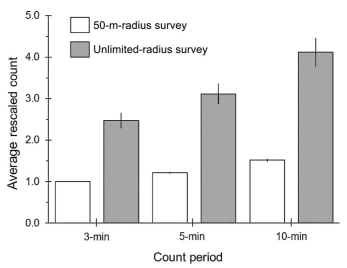
\includegraphics[width=0.8\linewidth]{images/matsuoka-2014-fig-2} \caption{Effects of duration and distance on mean counts, from [@matsuoka2014].}\label{fig:intro-1}
\end{figure}

Point counts are commonly used to answer questions like:

\begin{itemize}
\tightlist
\item
  How many? (Abundance, density, population size)
\item
  Is this location part of the range? (0/1)
\item
  How is abundance changing in space? (Distribution)
\item
  How is abundance changing in time? (Trend)
\item
  What is the effect of a treatment on abundance?
\end{itemize}

\hypertarget{design-based-approaches}{%
\section{Design-based approaches}\label{design-based-approaches}}

Standards and recommendations can
maximize efficiency in the numbers of birds and species counted,
minimize extraneous variability in the counts.

But programs started to deviate from standards:
\emph{``For example, only 3\% of 196,000 point counts conducted during the period
1992--2011 across Alaska and Canada followed the standards recommended for the count period and count radius''} (\citep{matsuoka2014}).
Figure \ref{fig:intro-2} show how point count protocol varies
across the boreal region of North America.

\begin{figure}
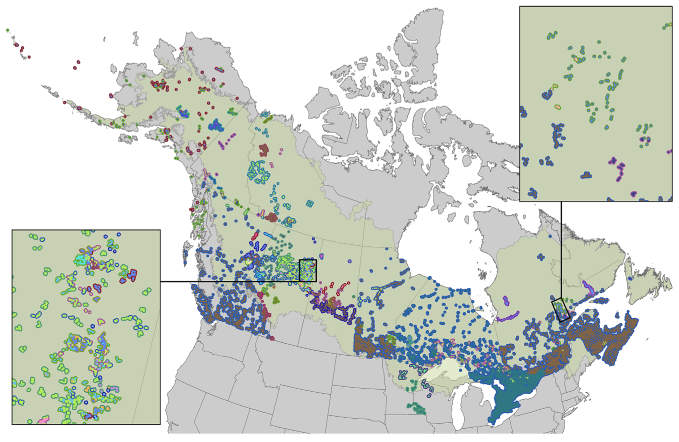
\includegraphics[width=0.8\linewidth]{images/barker-2015-fig-2} \caption{Survey methodology variation (colors) among contributed projects in the Boreal Avian Modelling (BAM) data base, from [@barker2015].}\label{fig:intro-2}
\end{figure}

\BeginKnitrBlock{rmdexercise}
\textbf{Exercise}

In what regard can protocols differ?

What might drive protocol variation among projects?

Why have we abandoned following protocols?
\EndKnitrBlock{rmdexercise}

\hypertarget{model-based-approaches}{%
\section{Model-based approaches}\label{model-based-approaches}}

Detection probabilities might vary even with fixed effort
(we'll cover this more later),
and programs might have their own goals and constraints (access, training, etc).
These constraints would make it almost impossible, and potentially costly
to set up very specific standards.

Labour intensive methods for unmarked populations
have come to the forefront, and computing power of
personal computers opened the door for model-based approaches,
that can accomodate more variation given enough information
in the observed data. These methods often rely on ancillary
information and often some sort of replication.

Some of the commonly used model-based approaches are:

\begin{itemize}
\tightlist
\item
  double observer (\href{https://doi.org/10.1642/0004-8038(2000)117\%5B0393:ADOAFE\%5D2.0.CO;2}{Nichols et al.~2000}),
\item
  distance sampling (\href{https://global.oup.com/academic/product/introduction-to-distance-sampling-9780198509271}{Buckland et al.~2001}),
\item
  removal sampling (\href{https://doi.org/10.1642/0004-8038(2002)119\%5B0414:ARMFED\%5D2.0.CO;2}{Farnsworth et al.~2002}),
\item
  multiple visit occupancy (\href{https://doi.org/10.1890/0012-9658(2002)083\%5B2248:ESORWD\%5D2.0.CO;2}{MacKenzie et al.~2002}),
\item
  multiple visit abundance (\href{https://doi.org/10.1111/j.0006-341X.2004.00142.x}{Royle 2004}).
\end{itemize}

Models come with assumptions, such as:

\begin{itemize}
\tightlist
\item
  population is closed during multiple visits,
\item
  observers are independent,
\item
  all individuals emit cues with identical rates,
\item
  spatial distribution of individuals is uniform,
\item
  etc.
\end{itemize}

Although assumptions are everywhere, we are really good at ignoring
and violating them.

\BeginKnitrBlock{rmdexercise}
\textbf{Exercise}

Can you mention some assumptions from everyday life?

Can you explain why we neglect/violate assumptions in these situations?
\EndKnitrBlock{rmdexercise}

Assumptions are violated, because we seek simplicity.
The main question we have to ask: \emph{does it matter in practice} if
we violate the assumptions?

\hypertarget{our-approach}{%
\section{Our approach}\label{our-approach}}

In this book and course, we will critically evaluate common assumptions made
when analyzing point count data using the following approach:

\begin{enumerate}
\def\labelenumi{\arabic{enumi}.}
\tightlist
\item
  we will introduce a concept,
\item
  understand how we can infer it from data,
\item
  then we recreate the situation \emph{in silico},
\item
  and see how the outcome changes as we make different assumptions.
\end{enumerate}

It is guaranteed that we will violate every assumption we make.
To get away with it, we need to understand how much is too much,
and whether it has an impact in practice.
If there is a practical consequence, we will look at ways to minimize
that effects -- so that we can safely ignore the assumption.

\hypertarget{pcdata}{%
\chapter{Organizing and Processing Point Count Data}\label{pcdata}}

\begin{quote}
All data are messy, but some are missing
\end{quote}

\hypertarget{introduction}{%
\section{Introduction}\label{introduction}}

It is often called \emph{data processing}, \emph{data munging},
\emph{data wrangling}, \emph{data cleaning}.
None of these expressions capture the dread associated with the actual activity.
Luckily, this book and course is not about data manipulation,
and we can gladly skip these steps. But keep in mind,
in real life, you'll often have to worry about at least four things
that can go wrong:

\begin{enumerate}
\def\labelenumi{\arabic{enumi}.}
\tightlist
\item
  space (e.g.~wrong UTM zones, errors),
\item
  time (ISO format please),
\item
  taxonomy (unknowns, mis-identifications),
\item
  something else (if there were no errors, check again).
\end{enumerate}

This chapter sets you up for the required data skills for the
rest of the book/course.

\hypertarget{prerequisites}{%
\section{Prerequisites}\label{prerequisites}}

\begin{Shaded}
\begin{Highlighting}[]
\KeywordTok{library}\NormalTok{(mefa4)                }\CommentTok{# data manipulation}
\KeywordTok{library}\NormalTok{(raster)               }\CommentTok{# reading raster files}
\KeywordTok{library}\NormalTok{(sp)                   }\CommentTok{# spatial data manipulation}
\KeywordTok{load}\NormalTok{(}\StringTok{"_data/josm/josm.rda"}\NormalTok{)   }\CommentTok{# load bird data}
\NormalTok{rr <-}\StringTok{ }\KeywordTok{stack}\NormalTok{(}\StringTok{"_data/josm/landcover-hfi2016.grd"}\NormalTok{) }\CommentTok{# rasters}
\end{Highlighting}
\end{Shaded}

\hypertarget{rbasics}{%
\section{R basics}\label{rbasics}}

This short document is intended to help you brush up your R skills.
If you feel that these R basics are not very familiar,
I suggest to take a look at some introductory R books,
sich as this preprint version of Norman Matloff's \emph{The Art of R Programming} book: \url{http://heather.cs.ucdavis.edu/~matloff/132/NSPpart.pdf}, check out Chapters 1--6.

R is a great calculator:

\begin{Shaded}
\begin{Highlighting}[]
\DecValTok{1} \OperatorTok{+}\StringTok{ }\DecValTok{2}
\end{Highlighting}
\end{Shaded}

Assign a value and print an object using \texttt{=} or \texttt{\textless{}-} (preferred in this book):

\begin{Shaded}
\begin{Highlighting}[]
\NormalTok{(}\DataTypeTok{x =} \DecValTok{2}\NormalTok{) }\CommentTok{# shorthand for print}
\KeywordTok{print}\NormalTok{(x)}
\NormalTok{x }\OperatorTok{==}\StringTok{ }\DecValTok{2} \CommentTok{# logical operator, not assignment}
\NormalTok{y <-}\StringTok{ }\NormalTok{x }\OperatorTok{+}\StringTok{ }\FloatTok{0.5}
\NormalTok{y }\CommentTok{# another way to print}
\end{Highlighting}
\end{Shaded}

Logical operators come handy:

\begin{Shaded}
\begin{Highlighting}[]
\NormalTok{x }\OperatorTok{==}\StringTok{ }\NormalTok{y }\CommentTok{# equal}
\NormalTok{x }\OperatorTok{!=}\StringTok{ }\NormalTok{y }\CommentTok{# not eaqual}
\NormalTok{x }\OperatorTok{<}\StringTok{ }\NormalTok{y }\CommentTok{# smaller than}
\NormalTok{x }\OperatorTok{>=}\StringTok{ }\NormalTok{y }\CommentTok{# greater than or equal}
\end{Highlighting}
\end{Shaded}

Vectors and sequences are created most often by the functions
\texttt{c}, \texttt{:}, \texttt{seq}, and \texttt{rep}:

\begin{Shaded}
\begin{Highlighting}[]
\NormalTok{x <-}\StringTok{ }\KeywordTok{c}\NormalTok{(}\DecValTok{1}\NormalTok{, }\DecValTok{2}\NormalTok{, }\DecValTok{3}\NormalTok{)}
\NormalTok{x}
\DecValTok{1}\OperatorTok{:}\DecValTok{3}
\KeywordTok{seq}\NormalTok{(}\DecValTok{1}\NormalTok{, }\DecValTok{3}\NormalTok{, }\DataTypeTok{by =} \DecValTok{1}\NormalTok{)}

\KeywordTok{rep}\NormalTok{(}\DecValTok{1}\NormalTok{, }\DecValTok{5}\NormalTok{)}
\KeywordTok{rep}\NormalTok{(}\DecValTok{1}\OperatorTok{:}\DecValTok{2}\NormalTok{, }\DecValTok{5}\NormalTok{)}
\KeywordTok{rep}\NormalTok{(}\DecValTok{1}\OperatorTok{:}\DecValTok{2}\NormalTok{, }\DataTypeTok{each =} \DecValTok{5}\NormalTok{)}
\end{Highlighting}
\end{Shaded}

When doing operations with vectors remember that values of
the shorter object are recycled:

\begin{Shaded}
\begin{Highlighting}[]
\NormalTok{x }\OperatorTok{+}\StringTok{ }\FloatTok{0.5}
\NormalTok{x }\OperatorTok{*}\StringTok{ }\KeywordTok{c}\NormalTok{(}\DecValTok{10}\NormalTok{, }\DecValTok{11}\NormalTok{, }\DecValTok{12}\NormalTok{, }\DecValTok{13}\NormalTok{)}
\end{Highlighting}
\end{Shaded}

Indexing and ordering vectors is a a fundamental skill:

\begin{Shaded}
\begin{Highlighting}[]
\NormalTok{x[}\DecValTok{1}\NormalTok{]}
\NormalTok{x[}\KeywordTok{c}\NormalTok{(}\DecValTok{1}\NormalTok{, }\DecValTok{1}\NormalTok{, }\DecValTok{1}\NormalTok{)] }\CommentTok{# a way of repeatig values}
\NormalTok{x[}\DecValTok{1}\OperatorTok{:}\DecValTok{2}\NormalTok{]}
\NormalTok{x[x }\OperatorTok{!=}\StringTok{ }\DecValTok{2}\NormalTok{]}
\NormalTok{x[x }\OperatorTok{==}\StringTok{ }\DecValTok{2}\NormalTok{]}
\NormalTok{x[x }\OperatorTok{>}\StringTok{ }\DecValTok{1} \OperatorTok{&}\StringTok{ }\NormalTok{x }\OperatorTok{<}\StringTok{ }\DecValTok{3}\NormalTok{]}
\KeywordTok{order}\NormalTok{(x, }\DataTypeTok{decreasing=}\OtherTok{TRUE}\NormalTok{)}
\NormalTok{x[}\KeywordTok{order}\NormalTok{(x, }\DataTypeTok{decreasing=}\OtherTok{TRUE}\NormalTok{)]}
\KeywordTok{rev}\NormalTok{(x) }\CommentTok{# reverse}
\end{Highlighting}
\end{Shaded}

See how \texttt{NA} values can influence
sorting character vectors:

\begin{Shaded}
\begin{Highlighting}[]
\NormalTok{z <-}\StringTok{ }\KeywordTok{c}\NormalTok{(}\StringTok{"b"}\NormalTok{, }\StringTok{"a"}\NormalTok{, }\StringTok{"c"}\NormalTok{, }\OtherTok{NA}\NormalTok{)}
\NormalTok{z[z }\OperatorTok{==}\StringTok{ "a"}\NormalTok{]}
\NormalTok{z[}\OperatorTok{!}\KeywordTok{is.na}\NormalTok{(z) }\OperatorTok{&}\StringTok{ }\NormalTok{z }\OperatorTok{==}\StringTok{ "a"}\NormalTok{]}
\NormalTok{z[}\KeywordTok{is.na}\NormalTok{(z) }\OperatorTok{|}\StringTok{ }\NormalTok{z }\OperatorTok{==}\StringTok{ "a"}\NormalTok{]}
\KeywordTok{is.na}\NormalTok{(z)}
\KeywordTok{which}\NormalTok{(}\KeywordTok{is.na}\NormalTok{(z))}
\KeywordTok{sort}\NormalTok{(z)}
\KeywordTok{sort}\NormalTok{(z, }\DataTypeTok{na.last=}\OtherTok{TRUE}\NormalTok{)}
\end{Highlighting}
\end{Shaded}

There are a few special values:

\begin{Shaded}
\begin{Highlighting}[]
\KeywordTok{as.numeric}\NormalTok{(}\KeywordTok{c}\NormalTok{(}\StringTok{"1"}\NormalTok{, }\StringTok{"a"}\NormalTok{)) }\CommentTok{# NA: not available (missing or invalid)}
\DecValTok{0}\OperatorTok{/}\DecValTok{0} \CommentTok{# NaN: not a number}
\DecValTok{1}\OperatorTok{/}\DecValTok{0} \CommentTok{# Inf}
\DecValTok{-1}\OperatorTok{/}\DecValTok{0} \CommentTok{# -Inf}
\end{Highlighting}
\end{Shaded}

Matrices and arrays are vectors with dimensions, elements are in same mode:

\begin{Shaded}
\begin{Highlighting}[]
\NormalTok{(m <-}\StringTok{ }\KeywordTok{matrix}\NormalTok{(}\DecValTok{1}\OperatorTok{:}\DecValTok{12}\NormalTok{, }\DecValTok{4}\NormalTok{, }\DecValTok{3}\NormalTok{))}
\KeywordTok{matrix}\NormalTok{(}\DecValTok{1}\OperatorTok{:}\DecValTok{12}\NormalTok{, }\DecValTok{4}\NormalTok{, }\DecValTok{3}\NormalTok{, }\DataTypeTok{byrow=}\OtherTok{TRUE}\NormalTok{)}

\KeywordTok{array}\NormalTok{(}\DecValTok{1}\OperatorTok{:}\DecValTok{12}\NormalTok{, }\KeywordTok{c}\NormalTok{(}\DecValTok{2}\NormalTok{, }\DecValTok{2}\NormalTok{, }\DecValTok{3}\NormalTok{))}
\end{Highlighting}
\end{Shaded}

Many objects have attributes:

\begin{Shaded}
\begin{Highlighting}[]
\KeywordTok{dim}\NormalTok{(m)}
\KeywordTok{dim}\NormalTok{(m) <-}\StringTok{ }\OtherTok{NULL}
\NormalTok{m}
\KeywordTok{dim}\NormalTok{(m) <-}\StringTok{ }\KeywordTok{c}\NormalTok{(}\DecValTok{4}\NormalTok{, }\DecValTok{3}\NormalTok{)}
\NormalTok{m}
\KeywordTok{dimnames}\NormalTok{(m) <-}\StringTok{ }\KeywordTok{list}\NormalTok{(letters[}\DecValTok{1}\OperatorTok{:}\DecValTok{4}\NormalTok{], LETTERS[}\DecValTok{1}\OperatorTok{:}\DecValTok{3}\NormalTok{])}
\NormalTok{m}
\KeywordTok{attributes}\NormalTok{(m)}
\end{Highlighting}
\end{Shaded}

Matrice and indices:

\begin{Shaded}
\begin{Highlighting}[]
\NormalTok{m[}\DecValTok{1}\OperatorTok{:}\DecValTok{2}\NormalTok{,]}
\NormalTok{m[}\DecValTok{1}\NormalTok{,}\DecValTok{2}\NormalTok{]}
\NormalTok{m[,}\DecValTok{2}\NormalTok{]}
\NormalTok{m[,}\DecValTok{2}\NormalTok{,drop=}\OtherTok{FALSE}\NormalTok{]}
\NormalTok{m[}\DecValTok{2}\NormalTok{]}

\NormalTok{m[}\KeywordTok{rownames}\NormalTok{(m) }\OperatorTok{==}\StringTok{ "c"}\NormalTok{,]}
\NormalTok{m[}\KeywordTok{rownames}\NormalTok{(m) }\OperatorTok{!=}\StringTok{ "c"}\NormalTok{,]}
\NormalTok{m[}\KeywordTok{rownames}\NormalTok{(m) }\OperatorTok\StringTok{ }\KeywordTok{c}\NormalTok{(}\StringTok{"a"}\NormalTok{, }\StringTok{"c"}\NormalTok{, }\StringTok{"e"}\NormalTok{),]}
\NormalTok{m[}\OperatorTok{!}\NormalTok{(}\KeywordTok{rownames}\NormalTok{(m) }\OperatorTok\StringTok{ }\KeywordTok{c}\NormalTok{(}\StringTok{"a"}\NormalTok{, }\StringTok{"c"}\NormalTok{, }\StringTok{"e"}\NormalTok{)),]}
\end{Highlighting}
\end{Shaded}

Lists and indexing:

\begin{Shaded}
\begin{Highlighting}[]
\NormalTok{l <-}\StringTok{ }\KeywordTok{list}\NormalTok{(}\DataTypeTok{m =}\NormalTok{ m, }\DataTypeTok{x =}\NormalTok{ x, }\DataTypeTok{z =}\NormalTok{ z)}
\NormalTok{l}
\NormalTok{l}\OperatorTok{$}\NormalTok{ddd <-}\StringTok{ }\KeywordTok{sqrt}\NormalTok{(l}\OperatorTok{$}\NormalTok{x)}
\NormalTok{l[}\DecValTok{2}\OperatorTok{:}\DecValTok{3}\NormalTok{]}
\NormalTok{l[[}\StringTok{"ddd"}\NormalTok{]]}
\end{Highlighting}
\end{Shaded}

Data frames are often required for statistical modeling.
A data frame is a list where length of elements match and elements
can be in different mode.

\begin{Shaded}
\begin{Highlighting}[]
\NormalTok{d <-}\StringTok{ }\KeywordTok{data.frame}\NormalTok{(}\DataTypeTok{x =}\NormalTok{ x, }\DataTypeTok{sqrt_x =} \KeywordTok{sqrt}\NormalTok{(x))}
\NormalTok{d}
\end{Highlighting}
\end{Shaded}

Inspect structure of R objects:

\begin{Shaded}
\begin{Highlighting}[]
\KeywordTok{str}\NormalTok{(x)}
\KeywordTok{str}\NormalTok{(z)}
\KeywordTok{str}\NormalTok{(m)}
\KeywordTok{str}\NormalTok{(l)}
\KeywordTok{str}\NormalTok{(d)}
\KeywordTok{str}\NormalTok{(}\KeywordTok{as.data.frame}\NormalTok{(m))}
\KeywordTok{str}\NormalTok{(}\KeywordTok{as.list}\NormalTok{(d))}
\end{Highlighting}
\end{Shaded}

Get summaries of these objects:

\begin{Shaded}
\begin{Highlighting}[]
\KeywordTok{summary}\NormalTok{(x)}
\KeywordTok{summary}\NormalTok{(z)}
\KeywordTok{summary}\NormalTok{(m)}
\KeywordTok{summary}\NormalTok{(l)}
\KeywordTok{summary}\NormalTok{(d)}
\end{Highlighting}
\end{Shaded}

\hypertarget{josm-data-set}{%
\section{JOSM data set}\label{josm-data-set}}

The data is based on the project \emph{Cause-Effect Monitoring Migratory Landbirds at Regional Scales:
understand how boreal songbirds are affected by human activity in the oil sands area} (\ref{fig:data-1} and \ref{fig:data-2}, \citep{mahon2016}).
JOSM stands for Joint Oil Sands Monitoring.
Look at the source code in the \texttt{\_data/josm} directory of the book
if you are interested in data processing details.
We skip that for now.

\begin{figure}
\includegraphics[width=0.8\linewidth]{images/mahon-2016-fig-1} \caption{JOSM bird data survey locations from [@mahon2016].}\label{fig:data-1}
\end{figure}

\begin{figure}
\includegraphics[width=0.8\linewidth]{images/mahon-2016-fig-2} \caption{Survey area boundary, habitat types and human footprint mapping [@mahon2016].}\label{fig:data-2}
\end{figure}

Surveys were spatially replicated because:

\begin{itemize}
\tightlist
\item
  we want to make inferences about a population,
\item
  full census is out of reach,
\item
  thus we take a sample of the population
\item
  that is representative and random.
\item
  Ideally, sample size should be as large as possible,
\item
  it reduces variability and
\item
  increases statistical power.
\end{itemize}

Survey locations were pucked based on various criteria:

\begin{itemize}
\tightlist
\item
  stratification (land cover),
\item
  gradients (disturbance levels),
\item
  random location (control for unmeasured effects),
\item
  take into account historical surveys (avoid, or revisit),
\item
  access, cost (clusters).
\end{itemize}

The \texttt{josm} obejct is a list with 3 elements:

\begin{itemize}
\tightlist
\item
  \texttt{surveys}: data frame with survey specific information,
\item
  \texttt{species}: lookup table for species,
\item
  \texttt{counts}: individual counts by survey and species.
\end{itemize}

\begin{Shaded}
\begin{Highlighting}[]
\KeywordTok{names}\NormalTok{(josm)}
\end{Highlighting}
\end{Shaded}

\begin{verbatim}
## [1] "surveys" "species" "counts"
\end{verbatim}

Species info: species codes, common and scientific names. The table could also contain
taxonomic, trait, etc. information as well.

\begin{Shaded}
\begin{Highlighting}[]
\KeywordTok{head}\NormalTok{(josm}\OperatorTok{$}\NormalTok{species)}
\end{Highlighting}
\end{Shaded}

At the survey level, we have coordinates, date/time info,
variables capturing survey conditions, and land cover info extracted from 1 km\(^2\) resolution rasters.

\begin{Shaded}
\begin{Highlighting}[]
\KeywordTok{colnames}\NormalTok{(josm}\OperatorTok{$}\NormalTok{surveys)}
\end{Highlighting}
\end{Shaded}

\begin{verbatim}
##  [1] "SiteID"        "SurveyArea"    "Longitude"     "Latitude"     
##  [5] "Date"          "StationID"     "ObserverID"    "TimeStart"    
##  [9] "VisitID"       "WindStart"     "PrecipStart"   "TempStart"    
## [13] "CloudStart"    "WindEnd"       "PrecipEnd"     "TempEnd"      
## [17] "CloudEnd"      "TimeFin"       "Noise"         "OvernightRain"
## [21] "DateTime"      "SunRiseTime"   "SunRiseFrac"   "TSSR"         
## [25] "OrdinalDay"    "DAY"           "Open"          "Water"        
## [29] "Agr"           "UrbInd"        "SoftLin"       "Roads"        
## [33] "Decid"         "OpenWet"       "Conif"         "ConifWet"
\end{verbatim}

The count table contains one row for each unique individual
of a species (\texttt{SpeciesID} links to the species lookup table)
observed during a survey (\texttt{StationID} links to the survey attribute table).
Check the data dictionary in \texttt{\_data/josm} folder for a detailed explanation of each column.

\begin{Shaded}
\begin{Highlighting}[]
\KeywordTok{str}\NormalTok{(josm}\OperatorTok{$}\NormalTok{counts)}
\end{Highlighting}
\end{Shaded}

\begin{verbatim}
## 'data.frame':    52372 obs. of  18 variables:
##  $ ObservationID: Factor w/ 57024 levels "CL10102-130622-001",..: 1 2 3 4 5 6 8 9 10 11 ...
##  $ SiteID       : Factor w/ 4569 levels "CL10102","CL10106",..: 1 1 1 1 1 1 1 1 2 2 ...
##  $ StationID    : Factor w/ 4569 levels "CL10102-1","CL10106-1",..: 1 1 1 1 1 1 1 1 2 2 ...
##  $ TimeInterval : int  1 1 1 1 5 5 1 1 1 1 ...
##  $ Direction    : int  1 2 2 2 1 4 4 4 1 1 ...
##  $ Distance     : int  1 2 2 1 3 3 2 1 1 1 ...
##  $ DetectType1  : Factor w/ 3 levels "C","S","V": 2 2 2 2 1 1 2 2 2 2 ...
##  $ DetectType2  : Factor w/ 3 levels "C","S","V": NA NA NA NA NA NA NA NA NA NA ...
##  $ DetectType3  : Factor w/ 3 levels "C","S","V": NA NA NA NA NA NA NA NA NA NA ...
##  $ Sex          : Factor w/ 4 levels "F","M","P","U": 2 2 2 2 4 4 2 2 2 2 ...
##  $ Age          : Factor w/ 6 levels "A","F","J","JUV",..: 1 1 1 1 1 1 1 1 1 1 ...
##  $ Activity1    : Factor w/ 17 levels "BE","CF","CH",..: 5 5 5 5 NA NA NA 5 5 NA ...
##  $ Activity2    : Factor w/ 17 levels "48","BE","CF",..: NA NA NA NA NA NA NA NA NA NA ...
##  $ Activity3    : Factor w/ 7 levels "CF","DC","DR",..: NA NA NA NA NA NA NA NA NA NA ...
##  $ ActivityNote : Factor w/ 959 levels "AGITATED","AGITATED CALLING",..: NA NA NA NA NA NA NA NA NA NA ...
##  $ Dur          : Factor w/ 3 levels "0-3min","3-5min",..: 1 1 1 1 3 3 1 1 1 1 ...
##  $ Dis          : Factor w/ 3 levels "0-50m","50-100m",..: 1 2 2 1 3 3 2 1 1 1 ...
##  $ SpeciesID    : Factor w/ 150 levels "ALFL","AMBI",..: 107 95 95 107 46 43 140 95 125 38 ...
\end{verbatim}

\hypertarget{cross-tabulating-species-counts}{%
\section{Cross tabulating species counts}\label{cross-tabulating-species-counts}}

Take the following dummy data frame (long format):

\begin{Shaded}
\begin{Highlighting}[]
\NormalTok{(d <-}\StringTok{ }\KeywordTok{data.frame}\NormalTok{(}
  \DataTypeTok{sample=}\KeywordTok{factor}\NormalTok{(}\KeywordTok{paste0}\NormalTok{(}\StringTok{"S"}\NormalTok{, }\KeywordTok{c}\NormalTok{(}\DecValTok{1}\NormalTok{,}\DecValTok{1}\NormalTok{,}\DecValTok{1}\NormalTok{,}\DecValTok{2}\NormalTok{,}\DecValTok{2}\NormalTok{)), }\KeywordTok{paste0}\NormalTok{(}\StringTok{"S"}\NormalTok{, }\DecValTok{1}\OperatorTok{:}\DecValTok{3}\NormalTok{)),}
  \DataTypeTok{species=}\KeywordTok{c}\NormalTok{(}\StringTok{"BTNW"}\NormalTok{, }\StringTok{"OVEN"}\NormalTok{, }\StringTok{"CANG"}\NormalTok{, }\StringTok{"AMRO"}\NormalTok{, }\StringTok{"CANG"}\NormalTok{),}
  \DataTypeTok{abundance=}\KeywordTok{c}\NormalTok{(}\DecValTok{1}\NormalTok{, }\DecValTok{1}\NormalTok{, }\DecValTok{2}\NormalTok{, }\DecValTok{1}\NormalTok{, }\DecValTok{1}\NormalTok{),}
  \DataTypeTok{behavior=}\KeywordTok{rep}\NormalTok{(}\KeywordTok{c}\NormalTok{(}\StringTok{"heard"}\NormalTok{,}\StringTok{"seen"}\NormalTok{), }\KeywordTok{c}\NormalTok{(}\DecValTok{4}\NormalTok{, }\DecValTok{1}\NormalTok{))))}
\KeywordTok{str}\NormalTok{(d)}
\end{Highlighting}
\end{Shaded}

\begin{verbatim}
## 'data.frame':    5 obs. of  4 variables:
##  $ sample   : Factor w/ 3 levels "S1","S2","S3": 1 1 1 2 2
##  $ species  : Factor w/ 4 levels "AMRO","BTNW",..: 2 4 3 1 3
##  $ abundance: num  1 1 2 1 1
##  $ behavior : Factor w/ 2 levels "heard","seen": 1 1 1 1 2
\end{verbatim}

We want to add up the \texttt{abundance}s for each sample (rows) and species (column):

\begin{Shaded}
\begin{Highlighting}[]
\NormalTok{(y <-}\StringTok{ }\KeywordTok{Xtab}\NormalTok{(abundance }\OperatorTok{~}\StringTok{ }\NormalTok{sample }\OperatorTok{+}\StringTok{ }\NormalTok{species, d))}
\end{Highlighting}
\end{Shaded}

\begin{verbatim}
## 3 x 4 sparse Matrix of class "dgCMatrix"
##    AMRO BTNW CANG OVEN
## S1    .    1    2    1
## S2    1    .    1    .
## S3    .    .    .    .
\end{verbatim}

\texttt{y} is a sparse matrix, that is a very compact representation:

\begin{Shaded}
\begin{Highlighting}[]
\KeywordTok{object.size}\NormalTok{(d[,}\DecValTok{1}\OperatorTok{:}\DecValTok{3}\NormalTok{])}
\end{Highlighting}
\end{Shaded}

\begin{verbatim}
## 2328 bytes
\end{verbatim}

\begin{Shaded}
\begin{Highlighting}[]
\KeywordTok{object.size}\NormalTok{(y)}
\end{Highlighting}
\end{Shaded}

\begin{verbatim}
## 2160 bytes
\end{verbatim}

Notice that we have 3 rows, but \texttt{d\$sample} did not have an \texttt{S3} value, but it was a level.
We can drop such unused levels, but it is generally not recommended, and we need to be careful
not to drop samples where no species was detected (this can happen quite often depending on timing of
surveys)

\begin{Shaded}
\begin{Highlighting}[]
\KeywordTok{Xtab}\NormalTok{(abundance }\OperatorTok{~}\StringTok{ }\NormalTok{sample }\OperatorTok{+}\StringTok{ }\NormalTok{species, d, }\DataTypeTok{drop.unused.levels =} \OtherTok{TRUE}\NormalTok{)}
\end{Highlighting}
\end{Shaded}

\begin{verbatim}
## 2 x 4 sparse Matrix of class "dgCMatrix"
##    AMRO BTNW CANG OVEN
## S1    .    1    2    1
## S2    1    .    1    .
\end{verbatim}

A sparse matrix can be converted to ordinary matrix

\begin{Shaded}
\begin{Highlighting}[]
\KeywordTok{as.matrix}\NormalTok{(y)}
\end{Highlighting}
\end{Shaded}

\begin{verbatim}
##    AMRO BTNW CANG OVEN
## S1    0    1    2    1
## S2    1    0    1    0
## S3    0    0    0    0
\end{verbatim}

The nice thing about this cross tabulation is that we can finter the records without
changing the structure (rows, columns) of the table:

\begin{Shaded}
\begin{Highlighting}[]
\KeywordTok{Xtab}\NormalTok{(abundance }\OperatorTok{~}\StringTok{ }\NormalTok{sample }\OperatorTok{+}\StringTok{ }\NormalTok{species, d[d}\OperatorTok{$}\NormalTok{behavior }\OperatorTok{==}\StringTok{ "heard"}\NormalTok{,])}
\end{Highlighting}
\end{Shaded}

\begin{verbatim}
## 3 x 4 sparse Matrix of class "dgCMatrix"
##    AMRO BTNW CANG OVEN
## S1    .    1    2    1
## S2    1    .    .    .
## S3    .    .    .    .
\end{verbatim}

\begin{Shaded}
\begin{Highlighting}[]
\KeywordTok{Xtab}\NormalTok{(abundance }\OperatorTok{~}\StringTok{ }\NormalTok{sample }\OperatorTok{+}\StringTok{ }\NormalTok{species, d[d}\OperatorTok{$}\NormalTok{behavior }\OperatorTok{==}\StringTok{ "seen"}\NormalTok{,])}
\end{Highlighting}
\end{Shaded}

\begin{verbatim}
## 3 x 4 sparse Matrix of class "dgCMatrix"
##    AMRO BTNW CANG OVEN
## S1    .    .    .    .
## S2    .    .    1    .
## S3    .    .    .    .
\end{verbatim}

Now let's do this for the real data. We have no abundance column, because
each row stands for exactly one individual. We can add a column with 1's,
or we can just count the number of rows by using only the right-hand-side of the
formula in \texttt{Xtab}. \texttt{ytot} will be our total count matrix for now.

We also want to filter the records to contain only \texttt{S}ongs and \texttt{C}alls, without
\texttt{V}visual detections:

\begin{Shaded}
\begin{Highlighting}[]
\KeywordTok{table}\NormalTok{(josm}\OperatorTok{$}\NormalTok{counts}\OperatorTok{$}\NormalTok{DetectType1, }\DataTypeTok{useNA=}\StringTok{"always"}\NormalTok{)}
\end{Highlighting}
\end{Shaded}

\begin{verbatim}
## 
##     C     S     V  <NA> 
##  9180 41808  1384     0
\end{verbatim}

We use \texttt{SiteID} for row names, because only 1 station and visit was done at each site:

\begin{Shaded}
\begin{Highlighting}[]
\NormalTok{ytot <-}\StringTok{ }\KeywordTok{Xtab}\NormalTok{(}\OperatorTok{~}\StringTok{ }\NormalTok{SiteID }\OperatorTok{+}\StringTok{ }\NormalTok{SpeciesID, josm}\OperatorTok{$}\NormalTok{counts[josm}\OperatorTok{$}\NormalTok{counts}\OperatorTok{$}\NormalTok{DetectType1 }\OperatorTok{!=}\StringTok{ "V"}\NormalTok{,])}
\end{Highlighting}
\end{Shaded}

See how not storing 0's affect size compared to the long formar and an ordinary wide matrix

\begin{Shaded}
\begin{Highlighting}[]
\CommentTok{## 2-column data frame as reference}
\NormalTok{tmp <-}\StringTok{ }\KeywordTok{as.numeric}\NormalTok{(}\KeywordTok{object.size}\NormalTok{(}
\NormalTok{  josm}\OperatorTok{$}\NormalTok{counts[josm}\OperatorTok{$}\NormalTok{counts}\OperatorTok{$}\NormalTok{DetectType1 }\OperatorTok{!=}\StringTok{ "V"}\NormalTok{, }\KeywordTok{c}\NormalTok{(}\StringTok{"StationID"}\NormalTok{, }\StringTok{"SpeciesID"}\NormalTok{)]))}
\CommentTok{## spare matrix}
\KeywordTok{as.numeric}\NormalTok{(}\KeywordTok{object.size}\NormalTok{(ytot)) }\OperatorTok{/}\StringTok{ }\NormalTok{tmp}
\end{Highlighting}
\end{Shaded}

\begin{verbatim}
## [1] 0.1366
\end{verbatim}

\begin{Shaded}
\begin{Highlighting}[]
\CommentTok{## dense matrix}
\KeywordTok{as.numeric}\NormalTok{(}\KeywordTok{object.size}\NormalTok{(}\KeywordTok{as.matrix}\NormalTok{(ytot))) }\OperatorTok{/}\StringTok{ }\NormalTok{tmp}
\end{Highlighting}
\end{Shaded}

\begin{verbatim}
## [1] 1.106
\end{verbatim}

\begin{Shaded}
\begin{Highlighting}[]
\CommentTok{## matrix fill}
\KeywordTok{sum}\NormalTok{(ytot }\OperatorTok{>}\StringTok{ }\DecValTok{0}\NormalTok{) }\OperatorTok{/}\StringTok{ }\KeywordTok{prod}\NormalTok{(}\KeywordTok{dim}\NormalTok{(ytot))}
\end{Highlighting}
\end{Shaded}

\begin{verbatim}
## [1] 0.04911
\end{verbatim}

Check if counts are as expected:

\begin{Shaded}
\begin{Highlighting}[]
\KeywordTok{max}\NormalTok{(ytot) }\CommentTok{# this is interesting}
\end{Highlighting}
\end{Shaded}

\begin{verbatim}
## [1] 200
\end{verbatim}

\begin{Shaded}
\begin{Highlighting}[]
\KeywordTok{sort}\NormalTok{(}\KeywordTok{apply}\NormalTok{(}\KeywordTok{as.matrix}\NormalTok{(ytot), }\DecValTok{2}\NormalTok{, max)) }\CommentTok{# it is CANG}
\end{Highlighting}
\end{Shaded}

\begin{verbatim}
## BUFF BWTE COGO COHA DCCO GWTE HOLA NHOW NSHO RTHU WWSC CANV NOPI AMBI AMCO 
##    0    0    0    0    0    0    0    0    0    0    0    0    0    1    1 
## AMGO BAEA BAOR BEKI BOWA CONI CSWA EAPH GBHE GCTH GGOW GHOW HOWR LEOW MERL 
##    1    1    1    1    1    1    1    1    1    1    1    1    1    1    1 
## NESP NOGO NOHA NSWO PBGR RBGU RTHA SAVS SPSA WBNU BRBL CAGU MYWA SNBU VEER 
##    1    1    1    1    1    1    1    1    1    1    1    1    1    1    1 
## AMKE AMWI BADO BARS BBWO BHCO BLBW BLPW BLTE BWHA COGR DOWO EAKI HAWO KILL 
##    2    2    2    2    2    2    2    2    2    2    2    2    2    2    2 
## LEYE NAWA NOPO OSFL OSPR PIWO PUFI RNDU SORA SSHA COSN AMCR AMRO ATTW BHVI 
##    2    2    2    2    2    2    2    2    2    2    2    3    3    3    3 
## BOCH BRCR BTNW CMWA FOSP FRGU GCKI MAWR MOWA NOFL PHVI SACR SOSA SOSP SPGR 
##    3    3    3    3    3    3    3    3    3    3    3    3    3    3    3 
## TRES WETA WIWA WIWR YBSA FOTE BAWW BBWA BCCH BLJA CAWA CONW COTE GRYE NOWA 
##    3    3    3    3    3    3    4    4    4    4    4    4    4    4    4 
## NRWS OCWA REVI RNGR RUBL RWBL WAVI WEWP WISN YBFL YWAR ALFL AMRE CHSP CORA 
##    4    4    4    4    4    4    4    4    4    4    4    5    5    5    5 
## EVGR HETH LCSP RBGR RBNU RCKI SWSP CCSP COYE DEJU LEFL LISP MAWA OVEN RUGR 
##    5    5    5    5    5    5    5    6    6    6    6    6    6    6    6 
## SWTH BOGU MALL GRAJ PAWA WTSP YRWA COLO TEWA AMPI WWCR CEDW PISI RECR CANG 
##    6    7    7    8    8    8    8    9   12   12   20   23   50   51  200
\end{verbatim}

\begin{Shaded}
\begin{Highlighting}[]
\CommentTok{## lyover (FO) flock (FL) beyond 100m distance}
\KeywordTok{head}\NormalTok{(josm}\OperatorTok{$}\NormalTok{counts[}
\NormalTok{  josm}\OperatorTok{$}\NormalTok{counts}\OperatorTok{$}\NormalTok{SiteID }\OperatorTok{==}\StringTok{ }\KeywordTok{rownames}\NormalTok{(ytot)[}\KeywordTok{which}\NormalTok{(ytot[,}\StringTok{"CANG"}\NormalTok{] }\OperatorTok{==}\StringTok{ }\DecValTok{200}\NormalTok{)] }\OperatorTok{&}
\StringTok{  }\NormalTok{josm}\OperatorTok{$}\NormalTok{counts}\OperatorTok{$}\NormalTok{SpeciesID }\OperatorTok{==}\StringTok{ "CANG"}\NormalTok{,])}
\end{Highlighting}
\end{Shaded}

We can check overall mean counts:

\begin{Shaded}
\begin{Highlighting}[]
\KeywordTok{round}\NormalTok{(}\KeywordTok{sort}\NormalTok{(}\KeywordTok{colMeans}\NormalTok{(ytot)), }\DecValTok{4}\NormalTok{)}
\end{Highlighting}
\end{Shaded}

\begin{verbatim}
##   BUFF   BWTE   COGO   COHA   DCCO   GWTE   HOLA   NHOW   NSHO   RTHU 
## 0.0000 0.0000 0.0000 0.0000 0.0000 0.0000 0.0000 0.0000 0.0000 0.0000 
##   WWSC   CANV   NOPI   GBHE   GCTH   GHOW   LEOW   NOHA   RBGU   BRBL 
## 0.0000 0.0000 0.0000 0.0002 0.0002 0.0002 0.0002 0.0002 0.0002 0.0002 
##   CAGU   AMCO   BAEA   BARS   NESP   NOGO   NOPO   NSWO   RNDU   SNBU 
## 0.0002 0.0004 0.0004 0.0004 0.0004 0.0004 0.0004 0.0004 0.0004 0.0004 
##   VEER   BEKI   CSWA   MERL   SAVS   SSHA   MYWA   AMKE   BAOR   OSPR 
## 0.0004 0.0007 0.0007 0.0007 0.0007 0.0007 0.0007 0.0009 0.0009 0.0009 
##   SPGR   WBNU   AMGO   AMWI   BOWA   CONI   EAPH   HOWR   NRWS   BLTE 
## 0.0009 0.0009 0.0011 0.0011 0.0011 0.0011 0.0011 0.0011 0.0011 0.0013 
##   COGR   EAKI   GGOW   NAWA   COSN   COTE   FRGU   MAWR   FOTE   KILL 
## 0.0013 0.0013 0.0013 0.0013 0.0013 0.0015 0.0015 0.0015 0.0015 0.0018 
##   RTHA   BADO   BLBW   AMBI   PBGR   SPSA   AMPI   BHCO   BWHA   SOSP 
## 0.0020 0.0024 0.0024 0.0028 0.0028 0.0028 0.0028 0.0031 0.0037 0.0042 
##   RUBL   MALL   PUFI   DOWO   SORA   LEYE   ATTW   HAWO   RNGR   BBWO 
## 0.0044 0.0046 0.0048 0.0059 0.0068 0.0094 0.0096 0.0101 0.0101 0.0107 
##   BLJA   BOGU   AMCR   EVGR   RWBL   OSFL   LCSP   TRES   FOSP   WEWP 
## 0.0134 0.0140 0.0166 0.0169 0.0169 0.0186 0.0193 0.0201 0.0217 0.0232 
##   WIWA   PIWO   RECR   SOSA   YWAR   GCKI   BLPW   CAWA   SACR   BTNW 
## 0.0236 0.0256 0.0269 0.0269 0.0291 0.0304 0.0306 0.0315 0.0322 0.0335 
##   NOWA   OCWA   BRCR   CCSP   COLO   PHVI   CONW   CEDW   RUGR   MOWA 
## 0.0341 0.0359 0.0381 0.0385 0.0387 0.0394 0.0429 0.0449 0.0475 0.0477 
##   WAVI   BCCH   BOCH   NOFL   SWSP   GRYE   WWCR   AMRO   RBNU   BBWA 
## 0.0582 0.0593 0.0593 0.0622 0.0659 0.0685 0.0751 0.0757 0.0766 0.0810 
##   CMWA   BHVI   COYE   YBFL   YBSA   AMRE   BAWW   LEFL   WETA   WISN 
## 0.0812 0.0814 0.0814 0.0873 0.0878 0.0889 0.0963 0.0974 0.1086 0.1280 
##   CORA   WIWR   ALFL   MAWA   PISI   RBGR   LISP   DEJU   GRAJ   CANG 
## 0.1401 0.1466 0.1582 0.1727 0.1775 0.1832 0.2169 0.2725 0.2898 0.3018 
##   PAWA   REVI   RCKI   HETH   CHSP   SWTH   WTSP   OVEN   YRWA   TEWA 
## 0.3053 0.3344 0.3898 0.4344 0.4460 0.7402 0.8091 0.8831 0.8934 1.2221
\end{verbatim}

\hypertarget{joining-species-data-with-predictors}{%
\section{Joining species data with predictors}\label{joining-species-data-with-predictors}}

Let's join the species counts with the survey attributes.
This is how we can prepare the input data for regression analysis.

\begin{Shaded}
\begin{Highlighting}[]
\NormalTok{spp <-}\StringTok{ "OVEN"} \CommentTok{# which species}
\NormalTok{josm}\OperatorTok{$}\NormalTok{species[spp,]}

\KeywordTok{compare_sets}\NormalTok{(}\KeywordTok{rownames}\NormalTok{(josm}\OperatorTok{$}\NormalTok{surveys),}\KeywordTok{rownames}\NormalTok{(ytot))}
\end{Highlighting}
\end{Shaded}

\begin{verbatim}
##        xlength ylength intersect union xbutnoty ybutnotx
## labels    4569    4569      4569  4569        0        0
## unique    4569    4569      4569  4569        0        0
\end{verbatim}

\begin{Shaded}
\begin{Highlighting}[]
\NormalTok{x <-}\StringTok{ }\NormalTok{josm}\OperatorTok{$}\NormalTok{surveys}
\NormalTok{x}\OperatorTok{$}\NormalTok{y <-}\StringTok{ }\KeywordTok{as.numeric}\NormalTok{(ytot[}\KeywordTok{rownames}\NormalTok{(x), spp])}
\end{Highlighting}
\end{Shaded}

\hypertarget{explore-predictor-variables}{%
\section{Explore predictor variables}\label{explore-predictor-variables}}

Put the locations on the map:

\begin{Shaded}
\begin{Highlighting}[]
\NormalTok{xy <-}\StringTok{ }\NormalTok{x[,}\KeywordTok{c}\NormalTok{(}\StringTok{"Longitude"}\NormalTok{, }\StringTok{"Latitude"}\NormalTok{)]}
\KeywordTok{coordinates}\NormalTok{(xy) <-}\StringTok{ }\ErrorTok{~}\StringTok{ }\NormalTok{Longitude }\OperatorTok{+}\StringTok{ }\NormalTok{Latitude}
\KeywordTok{proj4string}\NormalTok{(xy) <-}\StringTok{ "+proj=longlat +ellps=GRS80 +datum=NAD83 +no_defs"}
\NormalTok{xy <-}\StringTok{ }\KeywordTok{spTransform}\NormalTok{(xy, }\KeywordTok{proj4string}\NormalTok{(rr))}
\NormalTok{col <-}\StringTok{ }\KeywordTok{colorRampPalette}\NormalTok{(}\KeywordTok{c}\NormalTok{(}\StringTok{"lightgrey"}\NormalTok{, }\StringTok{"blue"}\NormalTok{))(}\DecValTok{100}\NormalTok{)}
\KeywordTok{plot}\NormalTok{(rr[[}\StringTok{"Water"}\NormalTok{]], }\DataTypeTok{col=}\NormalTok{col, }\DataTypeTok{axes=}\OtherTok{FALSE}\NormalTok{, }\DataTypeTok{box=}\OtherTok{FALSE}\NormalTok{, }\DataTypeTok{legend=}\OtherTok{FALSE}\NormalTok{)}
\KeywordTok{plot}\NormalTok{(xy, }\DataTypeTok{add=}\OtherTok{TRUE}\NormalTok{, }\DataTypeTok{pch=}\DecValTok{19}\NormalTok{, }\DataTypeTok{cex=}\FloatTok{0.5}\NormalTok{)}
\end{Highlighting}
\end{Shaded}

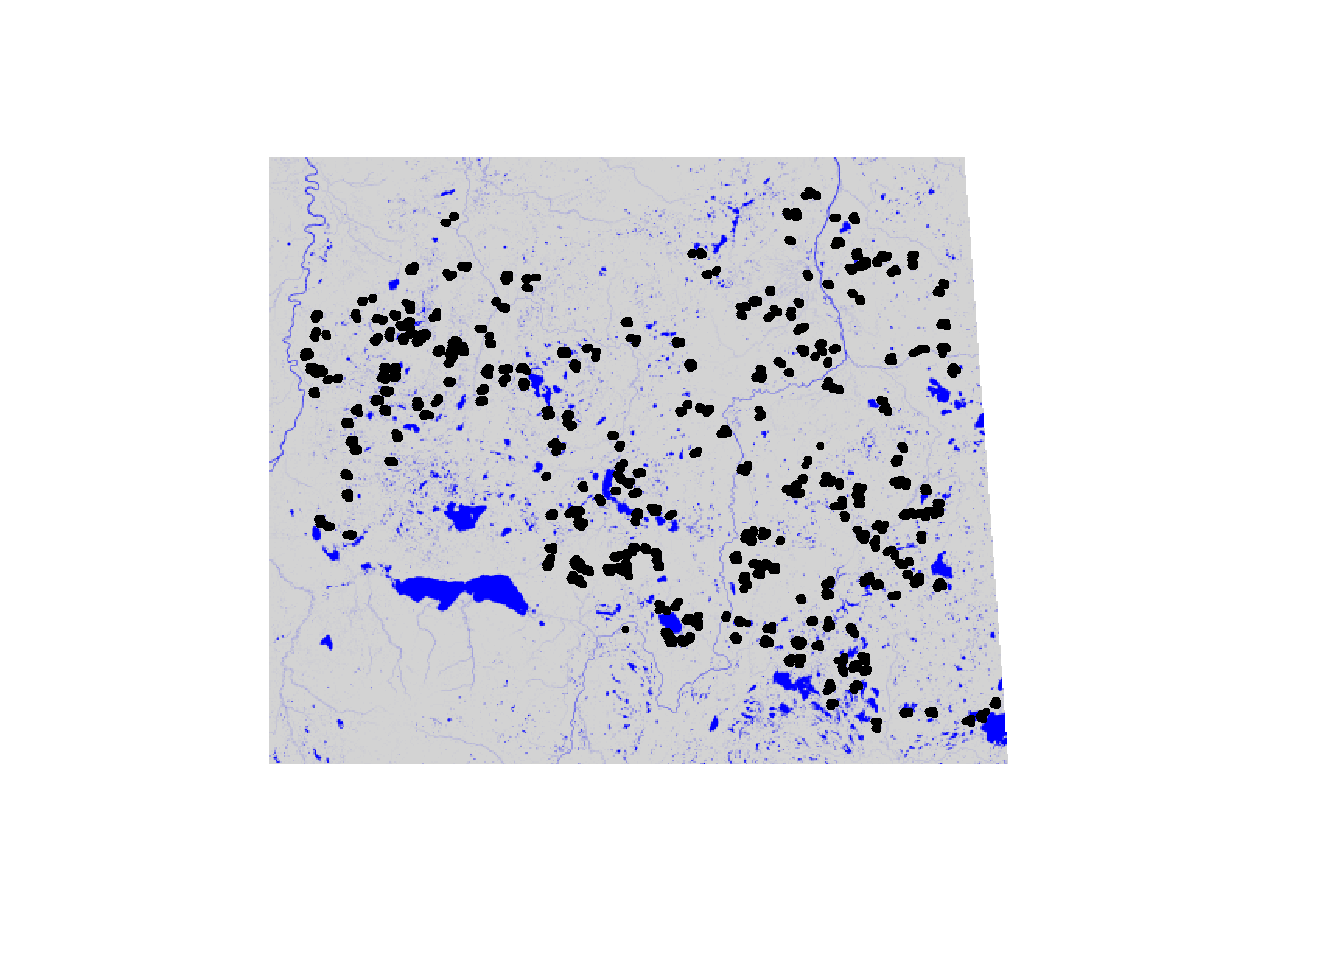
\includegraphics{qpad-book_files/figure-latex/data-xy-1.pdf}

\BeginKnitrBlock{rmdexercise}
\textbf{Exercise}

Explore the data to understand the distributions and associations.
Use \texttt{summary}, \texttt{table}, \texttt{hist}, \texttt{plot} (bivariate, scatterplot matrix), etc.
\EndKnitrBlock{rmdexercise}

\hypertarget{derived-variables}{%
\section{Derived variables}\label{derived-variables}}

Add up some of the compositional variables into meaningful units:

\begin{Shaded}
\begin{Highlighting}[]
\NormalTok{x}\OperatorTok{$}\NormalTok{FOR <-}\StringTok{ }\NormalTok{x}\OperatorTok{$}\NormalTok{Decid }\OperatorTok{+}\StringTok{ }\NormalTok{x}\OperatorTok{$}\NormalTok{Conif}\OperatorTok{+}\StringTok{ }\NormalTok{x}\OperatorTok{$}\NormalTok{ConifWet }\CommentTok{# forest}
\NormalTok{x}\OperatorTok{$}\NormalTok{AHF <-}\StringTok{ }\NormalTok{x}\OperatorTok{$}\NormalTok{Agr }\OperatorTok{+}\StringTok{ }\NormalTok{x}\OperatorTok{$}\NormalTok{UrbInd }\OperatorTok{+}\StringTok{ }\NormalTok{x}\OperatorTok{$}\NormalTok{Roads }\CommentTok{# 'alienating' human footprint}
\NormalTok{x}\OperatorTok{$}\NormalTok{WET <-}\StringTok{ }\NormalTok{x}\OperatorTok{$}\NormalTok{OpenWet }\OperatorTok{+}\StringTok{ }\NormalTok{x}\OperatorTok{$}\NormalTok{ConifWet }\OperatorTok{+}\StringTok{ }\NormalTok{x}\OperatorTok{$}\NormalTok{Water }\CommentTok{# wet + water}
\end{Highlighting}
\end{Shaded}

Classify surveys locations based on dominant land cover type:

\begin{Shaded}
\begin{Highlighting}[]
\NormalTok{cn <-}\StringTok{ }\KeywordTok{c}\NormalTok{(}\StringTok{"Open"}\NormalTok{, }\StringTok{"Water"}\NormalTok{, }\StringTok{"Agr"}\NormalTok{, }\StringTok{"UrbInd"}\NormalTok{, }\StringTok{"SoftLin"}\NormalTok{, }\StringTok{"Roads"}\NormalTok{, }\StringTok{"Decid"}\NormalTok{, }
  \StringTok{"OpenWet"}\NormalTok{, }\StringTok{"Conif"}\NormalTok{, }\StringTok{"ConifWet"}\NormalTok{)}
\NormalTok{h <-}\StringTok{ }\KeywordTok{find_max}\NormalTok{(x[,cn])}
\KeywordTok{hist}\NormalTok{(h}\OperatorTok{$}\NormalTok{value)}
\end{Highlighting}
\end{Shaded}

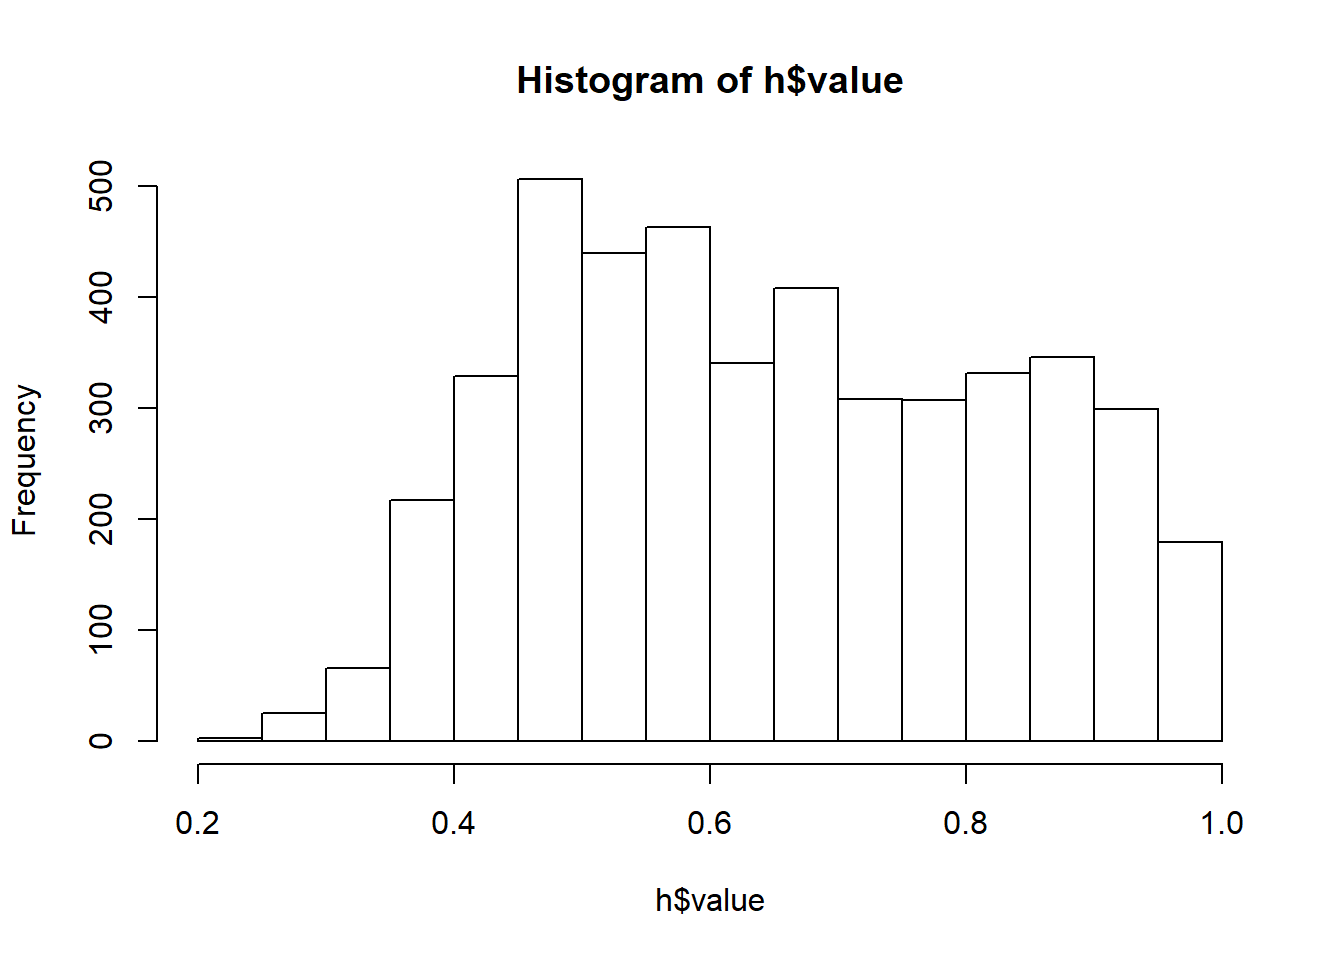
\includegraphics{qpad-book_files/figure-latex/data-deriv2-1.pdf}

\begin{Shaded}
\begin{Highlighting}[]
\KeywordTok{table}\NormalTok{(h}\OperatorTok{$}\NormalTok{index)}
\end{Highlighting}
\end{Shaded}

\begin{verbatim}
## 
##     Open    Water      Agr   UrbInd  SoftLin    Roads    Decid  OpenWet 
##       12       10        4       14        0        2     2084      160 
##    Conif ConifWet 
##      745     1538
\end{verbatim}

\begin{Shaded}
\begin{Highlighting}[]
\NormalTok{x}\OperatorTok{$}\NormalTok{HAB <-}\StringTok{ }\KeywordTok{droplevels}\NormalTok{(h}\OperatorTok{$}\NormalTok{index) }\CommentTok{# drop empty levels}
\end{Highlighting}
\end{Shaded}

\hypertarget{regression}{%
\chapter{A Primer in Regression Techniques}\label{regression}}

\begin{quote}
All models are wrong, but some are useful -- Box
\end{quote}

\hypertarget{introduction-1}{%
\section{Introduction}\label{introduction-1}}

This chapter will provide all the foundations we need for the coming chapters.
It is not intended as a general and all-exhaustive introduction to
regression techniques, but rather the minimum requirement moving forwards.
We will also hone our data processing and plotting skills.

\hypertarget{prerequisites-1}{%
\section{Prerequisites}\label{prerequisites-1}}

\begin{Shaded}
\begin{Highlighting}[]
\KeywordTok{library}\NormalTok{(mefa4)                }\CommentTok{# data manipulation}
\KeywordTok{library}\NormalTok{(mgcv)                 }\CommentTok{# GAMs}
\KeywordTok{library}\NormalTok{(pscl)                 }\CommentTok{# zero-inflated models}
\KeywordTok{library}\NormalTok{(lme4)                 }\CommentTok{# GLMMs}
\KeywordTok{library}\NormalTok{(MASS)                 }\CommentTok{# Negative Binomial GLM}
\KeywordTok{library}\NormalTok{(partykit)             }\CommentTok{# regression trees}
\KeywordTok{library}\NormalTok{(intrval)              }\CommentTok{# interval magic}
\KeywordTok{library}\NormalTok{(opticut)              }\CommentTok{# optimal partitioning}
\KeywordTok{library}\NormalTok{(visreg)               }\CommentTok{# regression visualization}
\KeywordTok{library}\NormalTok{(ResourceSelection)    }\CommentTok{# marginal effects}
\KeywordTok{library}\NormalTok{(MuMIn)                }\CommentTok{# multi-model inference}
\KeywordTok{source}\NormalTok{(}\StringTok{"functions.R"}\NormalTok{)         }\CommentTok{# some useful stuff}
\KeywordTok{load}\NormalTok{(}\StringTok{"_data/josm/josm.rda"}\NormalTok{) }\CommentTok{# JOSM data}
\end{Highlighting}
\end{Shaded}

Let's pick a species, Ovenbird (\texttt{OVEN}), that is quite common and abundant in the data set.
We put together a little data set to work with:

\begin{Shaded}
\begin{Highlighting}[]
\NormalTok{spp <-}\StringTok{ "OVEN"}

\NormalTok{ytot <-}\StringTok{ }\KeywordTok{Xtab}\NormalTok{(}\OperatorTok{~}\StringTok{ }\NormalTok{SiteID }\OperatorTok{+}\StringTok{ }\NormalTok{SpeciesID, josm}\OperatorTok{$}\NormalTok{counts[josm}\OperatorTok{$}\NormalTok{counts}\OperatorTok{$}\NormalTok{DetectType1 }\OperatorTok{!=}\StringTok{ "V"}\NormalTok{,])}
\NormalTok{ytot <-}\StringTok{ }\NormalTok{ytot[,}\KeywordTok{colSums}\NormalTok{(ytot }\OperatorTok{>}\StringTok{ }\DecValTok{0}\NormalTok{) }\OperatorTok{>}\StringTok{ }\DecValTok{0}\NormalTok{]}
\NormalTok{x <-}\StringTok{ }\KeywordTok{data.frame}\NormalTok{(}
\NormalTok{  josm}\OperatorTok{$}\NormalTok{surveys, }
  \DataTypeTok{y=}\KeywordTok{as.numeric}\NormalTok{(ytot[}\KeywordTok{rownames}\NormalTok{(josm}\OperatorTok{$}\NormalTok{surveys), spp]))}
\NormalTok{x}\OperatorTok{$}\NormalTok{FOR <-}\StringTok{ }\NormalTok{x}\OperatorTok{$}\NormalTok{Decid }\OperatorTok{+}\StringTok{ }\NormalTok{x}\OperatorTok{$}\NormalTok{Conif}\OperatorTok{+}\StringTok{ }\NormalTok{x}\OperatorTok{$}\NormalTok{ConifWet }\CommentTok{# forest}
\NormalTok{x}\OperatorTok{$}\NormalTok{AHF <-}\StringTok{ }\NormalTok{x}\OperatorTok{$}\NormalTok{Agr }\OperatorTok{+}\StringTok{ }\NormalTok{x}\OperatorTok{$}\NormalTok{UrbInd }\OperatorTok{+}\StringTok{ }\NormalTok{x}\OperatorTok{$}\NormalTok{Roads }\CommentTok{# 'alienating' human footprint}
\NormalTok{x}\OperatorTok{$}\NormalTok{WET <-}\StringTok{ }\NormalTok{x}\OperatorTok{$}\NormalTok{OpenWet }\OperatorTok{+}\StringTok{ }\NormalTok{x}\OperatorTok{$}\NormalTok{ConifWet }\OperatorTok{+}\StringTok{ }\NormalTok{x}\OperatorTok{$}\NormalTok{Water }\CommentTok{# wet + water}
\NormalTok{cn <-}\StringTok{ }\KeywordTok{c}\NormalTok{(}\StringTok{"Open"}\NormalTok{, }\StringTok{"Water"}\NormalTok{, }\StringTok{"Agr"}\NormalTok{, }\StringTok{"UrbInd"}\NormalTok{, }\StringTok{"SoftLin"}\NormalTok{, }\StringTok{"Roads"}\NormalTok{, }\StringTok{"Decid"}\NormalTok{, }
  \StringTok{"OpenWet"}\NormalTok{, }\StringTok{"Conif"}\NormalTok{, }\StringTok{"ConifWet"}\NormalTok{)}
\NormalTok{x}\OperatorTok{$}\NormalTok{HAB <-}\StringTok{ }\KeywordTok{droplevels}\NormalTok{(}\KeywordTok{find_max}\NormalTok{(x[,cn])}\OperatorTok{$}\NormalTok{index) }\CommentTok{# drop empty levels}
\NormalTok{x}\OperatorTok{$}\NormalTok{DEC <-}\StringTok{ }\KeywordTok{ifelse}\NormalTok{(x}\OperatorTok{$}\NormalTok{HAB }\OperatorTok{==}\StringTok{ "Decid"}\NormalTok{, }\DecValTok{1}\NormalTok{, }\DecValTok{0}\NormalTok{)}

\KeywordTok{table}\NormalTok{(x}\OperatorTok{$}\NormalTok{y)}
\end{Highlighting}
\end{Shaded}

\begin{verbatim}
## 
##    0    1    2    3    4    5    6 
## 2493  883  656  363  132   29   13
\end{verbatim}

\hypertarget{poisson-null-model}{%
\section{Poisson null model}\label{poisson-null-model}}

The null model states that the expected values of the count at all locations
are identical: \(E[Y_i]=\lambda\) (\(i=1,...,n\)), where \(Y_i\) is a random variable
that follows a Poisson distribution with mean \(\lambda\):
\((Y_i \mid \lambda) \sim Poisson(\lambda)\).
The observation (\(y_i\)) is a realization of the random variables \(Y\) at site \(i\),
these observations are independent and identically distributed (i.i.d.),
and we have \(n\) observations in total.

Saying the the distribution is Poisson is an assumption in itself. For example
we assume that the variance equals the mean (\(V(\mu)=\mu\)).

\begin{Shaded}
\begin{Highlighting}[]
\NormalTok{mP0 <-}\StringTok{ }\KeywordTok{glm}\NormalTok{(y }\OperatorTok{~}\StringTok{ }\DecValTok{1}\NormalTok{, }\DataTypeTok{data=}\NormalTok{x, }\DataTypeTok{family=}\NormalTok{poisson)}
\KeywordTok{mean}\NormalTok{(x}\OperatorTok{$}\NormalTok{y)}
\end{Highlighting}
\end{Shaded}

\begin{verbatim}
## [1] 0.8831
\end{verbatim}

\begin{Shaded}
\begin{Highlighting}[]
\KeywordTok{mean}\NormalTok{(}\KeywordTok{fitted}\NormalTok{(mP0))}
\end{Highlighting}
\end{Shaded}

\begin{verbatim}
## [1] 0.8831
\end{verbatim}

\begin{Shaded}
\begin{Highlighting}[]
\KeywordTok{exp}\NormalTok{(}\KeywordTok{coef}\NormalTok{(mP0))}
\end{Highlighting}
\end{Shaded}

\begin{verbatim}
## (Intercept) 
##      0.8831
\end{verbatim}

\begin{Shaded}
\begin{Highlighting}[]
\KeywordTok{summary}\NormalTok{(mP0)}
\end{Highlighting}
\end{Shaded}

\begin{verbatim}
## 
## Call:
## glm(formula = y ~ 1, family = poisson, data = x)
## 
## Deviance Residuals: 
##    Min      1Q  Median      3Q     Max  
##  -1.33   -1.33   -1.33    1.02    3.57  
## 
## Coefficients:
##             Estimate Std. Error z value Pr(>|z|)    
## (Intercept)  -0.1243     0.0157   -7.89  2.9e-15 ***
## ---
## Signif. codes:  0 '***' 0.001 '**' 0.01 '*' 0.05 '.' 0.1 ' ' 1
## 
## (Dispersion parameter for poisson family taken to be 1)
## 
##     Null deviance: 7424.8  on 4568  degrees of freedom
## Residual deviance: 7424.8  on 4568  degrees of freedom
## AIC: 12573
## 
## Number of Fisher Scoring iterations: 6
\end{verbatim}

The \texttt{family=poisson} specification implicitly assumes that we use a logarithmic link functions,
that is to say that \(log(\lambda) = \beta_0\), or equivalently: \(\lambda = e^{\beta_0}\).
The mean of the observations equal the mean of the fitted values, as expected.

The logarithmic function is called the link function, its inverse, the exponential function
is called the inverse link function. The model family has these convenently stored for us:

\begin{Shaded}
\begin{Highlighting}[]
\NormalTok{mP0}\OperatorTok{$}\NormalTok{family}
\end{Highlighting}
\end{Shaded}

\begin{verbatim}
## 
## Family: poisson 
## Link function: log
\end{verbatim}

\begin{Shaded}
\begin{Highlighting}[]
\NormalTok{mP0}\OperatorTok{$}\NormalTok{family}\OperatorTok{$}\NormalTok{linkfun}
\end{Highlighting}
\end{Shaded}

\begin{verbatim}
## function (mu) 
## log(mu)
## <environment: namespace:stats>
\end{verbatim}

\begin{Shaded}
\begin{Highlighting}[]
\NormalTok{mP0}\OperatorTok{$}\NormalTok{family}\OperatorTok{$}\NormalTok{linkinv}
\end{Highlighting}
\end{Shaded}

\begin{verbatim}
## function (eta) 
## pmax(exp(eta), .Machine$double.eps)
## <environment: namespace:stats>
\end{verbatim}

\hypertarget{exploring-covariates}{%
\section{Exploring covariates}\label{exploring-covariates}}

Now, in the absence of info about species biology, we are looking at a blank page.
How should we proceed? What kind of covariate (linear predictor) should we use?
We can do a quick and dirty exploration to see what are the likely candidates.
We use a regression tree (\texttt{ctree} refers to conditional trees). It is
a nonparametric method based on binary recursive partitioning in a conditional inference framework.
This means that binary splits are made along the predictor variables,
and the explanatory power of the split is assessed based on how it
maximized difference between the splits and minimized the difference inside the splits.
It is called conditional, because every new split is conditional on the previous splits
(difference can be measured in many different ways, think e.g.~sum of squares).
The stopping rule in this implementation is based on permutation tests (see \texttt{?ctree} or details
and references).

\begin{Shaded}
\begin{Highlighting}[]
\NormalTok{mCT <-}\StringTok{ }\KeywordTok{ctree}\NormalTok{(y }\OperatorTok{~}\StringTok{ }\NormalTok{Open }\OperatorTok{+}\StringTok{ }\NormalTok{Water }\OperatorTok{+}\StringTok{ }\NormalTok{Agr }\OperatorTok{+}\StringTok{ }\NormalTok{UrbInd }\OperatorTok{+}\StringTok{ }\NormalTok{SoftLin }\OperatorTok{+}\StringTok{ }\NormalTok{Roads }\OperatorTok{+}\StringTok{ }
\StringTok{  }\NormalTok{Decid }\OperatorTok{+}\StringTok{ }\NormalTok{OpenWet }\OperatorTok{+}\StringTok{ }\NormalTok{Conif }\OperatorTok{+}\StringTok{ }\NormalTok{ConifWet, }\DataTypeTok{data=}\NormalTok{x)}
\KeywordTok{plot}\NormalTok{(mCT)}
\end{Highlighting}
\end{Shaded}

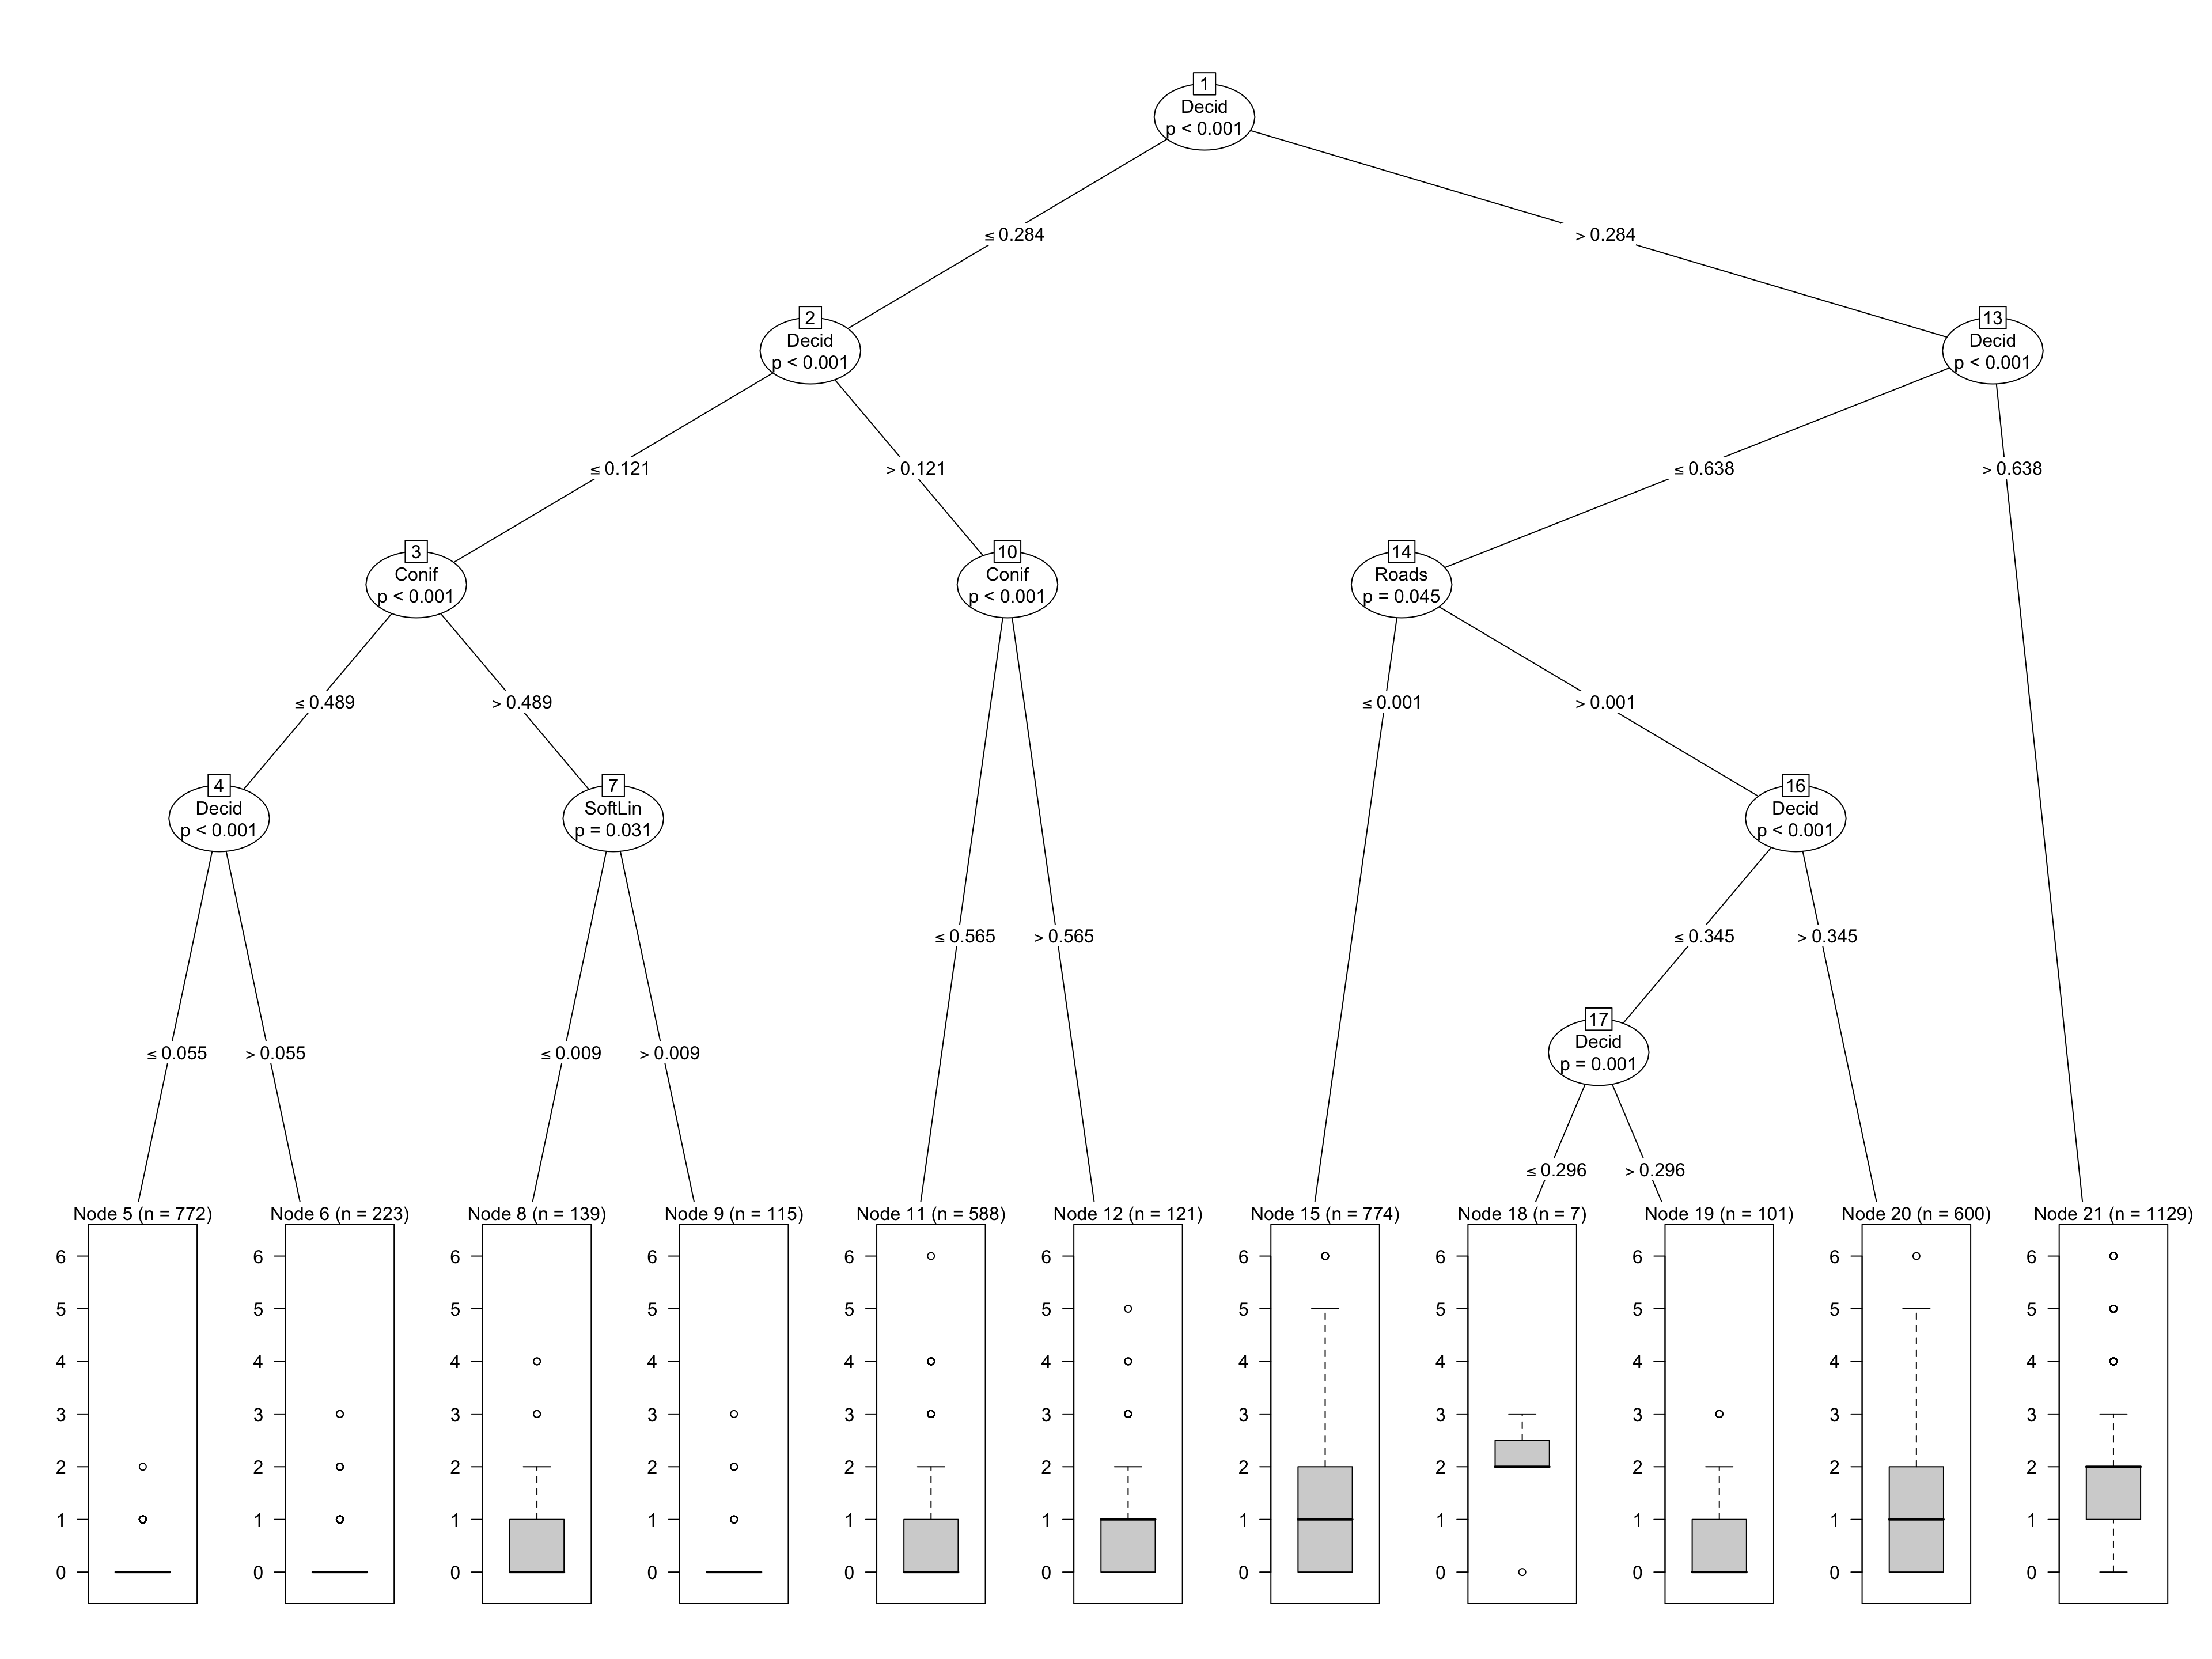
\includegraphics{qpad-book_files/figure-latex/regr-ctree-1.pdf}

The model can be seen as a piecewise constant regression, where each bucket (defined by
the splits along the tree) yields a constant predictions based on the mean of the
observations in the bucket. Any new data classified
into the same bucket will get the same value. There is no notion of uncertainty
(confidence or prediction intervals) in this nonparameric model.

But we see something very useful: the proportion of deciduous forest in the landscape
seems to be vary influential for Ovenbird abundance.

\hypertarget{single-covariate}{%
\section{Single covariate}\label{single-covariate}}

With this new found knowledge, let's fit a parametric (Poisson) linear model
using \texttt{Decid} as a predictor:

\begin{Shaded}
\begin{Highlighting}[]
\NormalTok{mP1 <-}\StringTok{ }\KeywordTok{glm}\NormalTok{(y }\OperatorTok{~}\StringTok{ }\NormalTok{Decid, }\DataTypeTok{data=}\NormalTok{x, }\DataTypeTok{family=}\NormalTok{poisson)}
\KeywordTok{mean}\NormalTok{(x}\OperatorTok{$}\NormalTok{y)}
\end{Highlighting}
\end{Shaded}

\begin{verbatim}
## [1] 0.8831
\end{verbatim}

\begin{Shaded}
\begin{Highlighting}[]
\KeywordTok{mean}\NormalTok{(}\KeywordTok{fitted}\NormalTok{(mP0))}
\end{Highlighting}
\end{Shaded}

\begin{verbatim}
## [1] 0.8831
\end{verbatim}

\begin{Shaded}
\begin{Highlighting}[]
\KeywordTok{coef}\NormalTok{(mP1)}
\end{Highlighting}
\end{Shaded}

\begin{verbatim}
## (Intercept)       Decid 
##      -1.164       2.134
\end{verbatim}

Same as before, the mean of the observations equal the mean of the fitted values.
But instead of only the intercapt, now we have 2 coefficients estimated.
Our linear predictor thus looks like:
\(log(\lambda_i) = \beta_0 + \beta_1 x_{1i}\). This means that expected abundance is
\(e^{\beta_0}\) where \texttt{Decid}=0,
\(e^{\beta_0}e^{\beta_1}\) where \texttt{Decid}=1,
and \(e^{\beta_0+\beta_1 x_{1}}\) in between.

The relationship can be visualized by plotting the fitted values against the predictor,
or using the coefficients to make predictions using our formula:

\begin{Shaded}
\begin{Highlighting}[]
\NormalTok{dec <-}\StringTok{ }\KeywordTok{seq}\NormalTok{(}\DecValTok{0}\NormalTok{, }\DecValTok{1}\NormalTok{, }\FloatTok{0.01}\NormalTok{)}
\NormalTok{lam <-}\StringTok{ }\KeywordTok{exp}\NormalTok{(}\KeywordTok{coef}\NormalTok{(mP1)[}\DecValTok{1}\NormalTok{] }\OperatorTok{+}\StringTok{ }\KeywordTok{coef}\NormalTok{(mP1)[}\DecValTok{2}\NormalTok{] }\OperatorTok{*}\StringTok{ }\NormalTok{dec)}
\KeywordTok{plot}\NormalTok{(}\KeywordTok{fitted}\NormalTok{(mP1) }\OperatorTok{~}\StringTok{ }\NormalTok{Decid, x, }\DataTypeTok{pch=}\DecValTok{19}\NormalTok{, }\DataTypeTok{col=}\StringTok{"grey"}\NormalTok{)}
\KeywordTok{lines}\NormalTok{(lam }\OperatorTok{~}\StringTok{ }\NormalTok{dec, }\DataTypeTok{col=}\DecValTok{2}\NormalTok{)}
\KeywordTok{rug}\NormalTok{(x}\OperatorTok{$}\NormalTok{Decid)}
\end{Highlighting}
\end{Shaded}

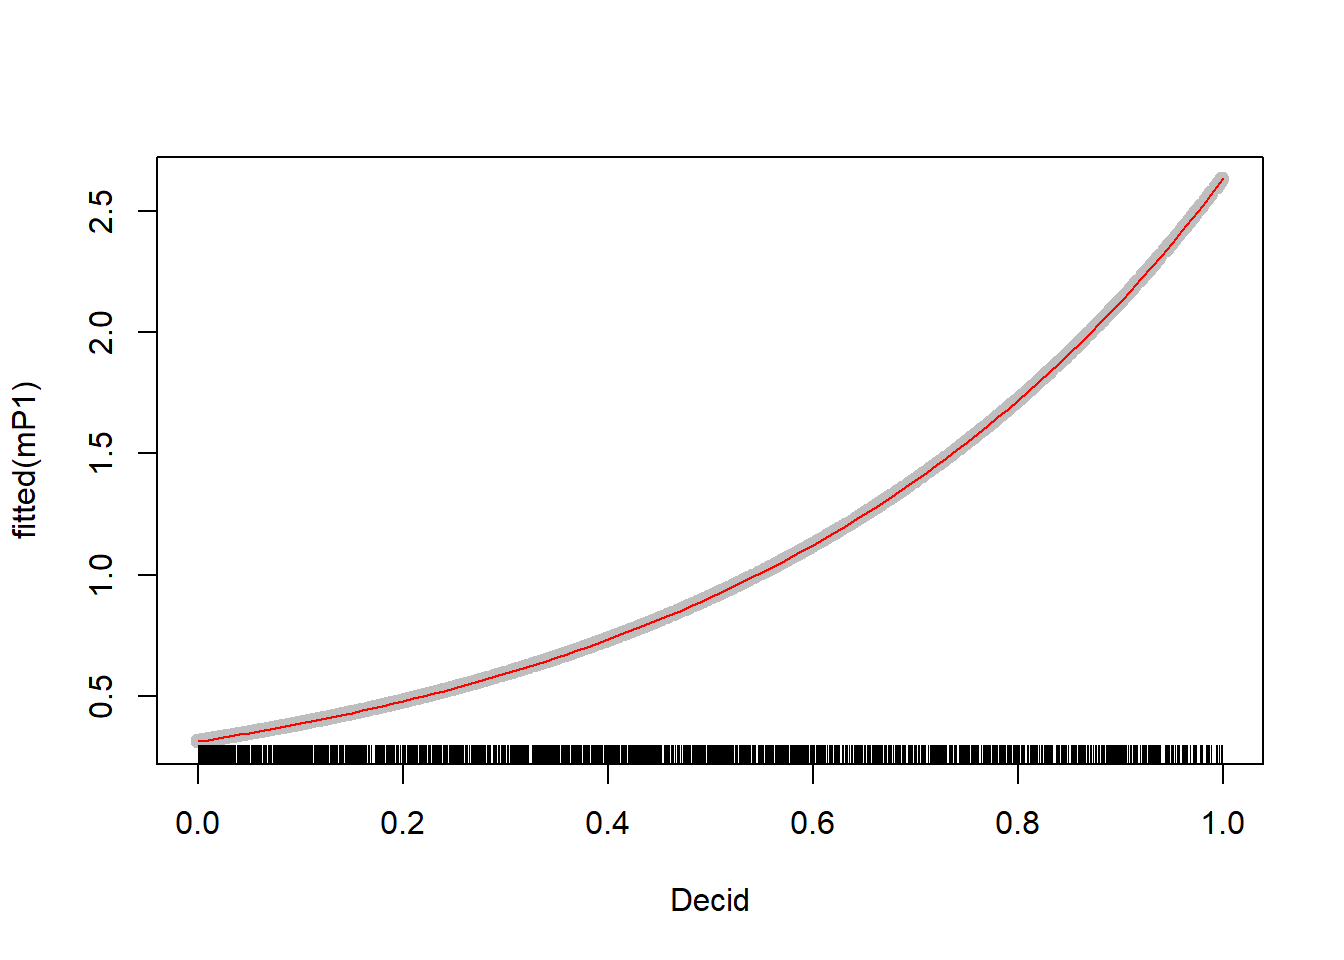
\includegraphics{qpad-book_files/figure-latex/regr-pois2_plot-1.pdf}

The model summary tells us that resudials are not quite right (we would expect
0 median and symmertic tails), in line with residual deviance
being much higher than residual degrees of freedom
(these should be close if the Poisson assumption holds).
But, the \texttt{Decid} effect is significant (meaning that the effect size is
large compared to the standard error):

\begin{Shaded}
\begin{Highlighting}[]
\KeywordTok{summary}\NormalTok{(mP1)}
\end{Highlighting}
\end{Shaded}

\begin{verbatim}
## 
## Call:
## glm(formula = y ~ Decid, family = poisson, data = x)
## 
## Deviance Residuals: 
##    Min      1Q  Median      3Q     Max  
## -2.291  -0.977  -0.790   0.469   4.197  
## 
## Coefficients:
##             Estimate Std. Error z value Pr(>|z|)    
## (Intercept)  -1.1643     0.0352   -33.1   <2e-16 ***
## Decid         2.1338     0.0537    39.7   <2e-16 ***
## ---
## Signif. codes:  0 '***' 0.001 '**' 0.01 '*' 0.05 '.' 0.1 ' ' 1
## 
## (Dispersion parameter for poisson family taken to be 1)
## 
##     Null deviance: 7424.8  on 4568  degrees of freedom
## Residual deviance: 5736.9  on 4567  degrees of freedom
## AIC: 10887
## 
## Number of Fisher Scoring iterations: 6
\end{verbatim}

We can compare this model to the null (constant, intercept-only) model:

\begin{Shaded}
\begin{Highlighting}[]
\KeywordTok{AIC}\NormalTok{(mP0, mP1)}
\KeywordTok{BIC}\NormalTok{(mP0, mP1)}
\KeywordTok{model.sel}\NormalTok{(mP0, mP1)}
\end{Highlighting}
\end{Shaded}

\begin{verbatim}
## Model selection table 
##     (Intrc) Decid df logLik  AICc delta weight
## mP1 -1.1640 2.134  2  -5442 10887     0      1
## mP0 -0.1243        1  -6285 12573  1686      0
## Models ranked by AICc(x)
\end{verbatim}

\begin{Shaded}
\begin{Highlighting}[]
\KeywordTok{R2dev}\NormalTok{(mP0, mP1)}
\end{Highlighting}
\end{Shaded}

\begin{verbatim}
##          R2   R2adj Deviance    Dev0    DevR     df0     dfR p_value    
## mP0    0.00    0.00     0.00 7424.78 7424.78 4568.00 4568.00  <2e-16 ***
## mP1    0.23    0.23  1687.87 7424.78 5736.91 4568.00 4567.00  <2e-16 ***
## ---
## Signif. codes:  0 '***' 0.001 '**' 0.01 '*' 0.05 '.' 0.1 ' ' 1
\end{verbatim}

AIC uses the negative log likelihood and the number of parameters as penalty.
Smaller value indicate a model that is closer to the (unknowable) true model
(caveat: this statement is true only asymptotically, i.e.~it holds for very large
sample sizes). For small samples, we of ten use BIC (more penalty for complex models
when sample size is small), or AICc (as in \texttt{MuMIn::model.sel}).

The other little table returned by \texttt{R2dev} shows deviance based (quasi) \(R^2\) and adjusted
\(R^2\) for some GLM classes, just for the sake of completeness. The Chi-squared based
test indicates good fit when the \(p\)-value is high (probability of being distributed
according the Poisson).

None of these two models is a particularly good fit in terms
of the parametric distribution.
This, however does not mean these models are not useful for making inferential statements
about ovenbirds. How useful these statements are, that is another question.
Let's dive into cinfidence and prediction intervals a bit.

\begin{Shaded}
\begin{Highlighting}[]
\NormalTok{B <-}\StringTok{ }\DecValTok{2000}
\NormalTok{alpha <-}\StringTok{ }\FloatTok{0.05}

\NormalTok{xnew <-}\StringTok{ }\KeywordTok{data.frame}\NormalTok{(}\DataTypeTok{Decid=}\KeywordTok{seq}\NormalTok{(}\DecValTok{0}\NormalTok{, }\DecValTok{1}\NormalTok{, }\FloatTok{0.01}\NormalTok{))}
\NormalTok{CI0 <-}\StringTok{ }\KeywordTok{predict_sim}\NormalTok{(mP0, xnew, }\DataTypeTok{interval=}\StringTok{"confidence"}\NormalTok{, }\DataTypeTok{level=}\DecValTok{1}\OperatorTok{-}\NormalTok{alpha, }\DataTypeTok{B=}\NormalTok{B)}
\NormalTok{PI0 <-}\StringTok{ }\KeywordTok{predict_sim}\NormalTok{(mP0, xnew, }\DataTypeTok{interval=}\StringTok{"prediction"}\NormalTok{, }\DataTypeTok{level=}\DecValTok{1}\OperatorTok{-}\NormalTok{alpha, }\DataTypeTok{B=}\NormalTok{B)}
\NormalTok{CI1 <-}\StringTok{ }\KeywordTok{predict_sim}\NormalTok{(mP1, xnew, }\DataTypeTok{interval=}\StringTok{"confidence"}\NormalTok{, }\DataTypeTok{level=}\DecValTok{1}\OperatorTok{-}\NormalTok{alpha, }\DataTypeTok{B=}\NormalTok{B)}
\NormalTok{PI1 <-}\StringTok{ }\KeywordTok{predict_sim}\NormalTok{(mP1, xnew, }\DataTypeTok{interval=}\StringTok{"prediction"}\NormalTok{, }\DataTypeTok{level=}\DecValTok{1}\OperatorTok{-}\NormalTok{alpha, }\DataTypeTok{B=}\NormalTok{B)}

\CommentTok{## nominal coverage is 95%}
\KeywordTok{sum}\NormalTok{(x}\OperatorTok{$}\NormalTok{y }\OperatorTok\StringTok{ }\KeywordTok{predict_sim}\NormalTok{(mP0, }\DataTypeTok{interval=}\StringTok{"prediction"}\NormalTok{, }\DataTypeTok{level=}\DecValTok{1}\OperatorTok{-}\NormalTok{alpha, }\DataTypeTok{B=}\NormalTok{B)[,}\KeywordTok{c}\NormalTok{(}\StringTok{"lwr"}\NormalTok{, }\StringTok{"upr"}\NormalTok{)]) }\OperatorTok{/}\StringTok{ }\KeywordTok{nrow}\NormalTok{(x)}
\end{Highlighting}
\end{Shaded}

\begin{verbatim}
## [1] 0.9619
\end{verbatim}

\begin{Shaded}
\begin{Highlighting}[]
\KeywordTok{sum}\NormalTok{(x}\OperatorTok{$}\NormalTok{y }\OperatorTok\StringTok{ }\KeywordTok{predict_sim}\NormalTok{(mP1, }\DataTypeTok{interval=}\StringTok{"prediction"}\NormalTok{, }\DataTypeTok{level=}\DecValTok{1}\OperatorTok{-}\NormalTok{alpha, }\DataTypeTok{B=}\NormalTok{B)[,}\KeywordTok{c}\NormalTok{(}\StringTok{"lwr"}\NormalTok{, }\StringTok{"upr"}\NormalTok{)]) }\OperatorTok{/}\StringTok{ }\KeywordTok{nrow}\NormalTok{(x)}
\end{Highlighting}
\end{Shaded}

\begin{verbatim}
## [1] 0.9711
\end{verbatim}

A model is said to have good \emph{coverage} when the prediction intervals
encompass the right amount of the observations. When the nominal level is 95\% (\(100 \times (1-\alpha)\),
where \(\alpha\) is Type I. error rate),
we expect 95\% of the observations fall within the 95\% \emph{prediction interval}.
The prediction interval includes the uncertainty around the coefficients
(confidence intervals, uncertainty in \(\hat{\lambda}\)) and the stochasticity coming from the
Poisson distribution (\(Y_i \sim Poisson(\hat{\lambda})\)).

The code above calculate the confidence and prediction intervals for the two models.
We also compared the prediction intervals and the nomial levels, and those were quite
close (ours being a bit more conservative), hinting that maybe the Poisson
distributional assumption is not very bad after all, but we'll come back to this later.

Let's see our confidence and prediction intervals for the two models:

\begin{Shaded}
\begin{Highlighting}[]
\NormalTok{yj <-}\StringTok{ }\KeywordTok{jitter}\NormalTok{(x}\OperatorTok{$}\NormalTok{y, }\FloatTok{0.5}\NormalTok{)}

\KeywordTok{plot}\NormalTok{(yj }\OperatorTok{~}\StringTok{ }\NormalTok{Decid, x, }\DataTypeTok{xlab=}\StringTok{"Decid"}\NormalTok{, }\DataTypeTok{ylab=}\StringTok{"E[Y]"}\NormalTok{,}
  \DataTypeTok{ylim=}\KeywordTok{c}\NormalTok{(}\DecValTok{0}\NormalTok{, }\KeywordTok{max}\NormalTok{(PI1}\OperatorTok{$}\NormalTok{upr)}\OperatorTok{+}\DecValTok{1}\NormalTok{), }\DataTypeTok{pch=}\DecValTok{19}\NormalTok{, }\DataTypeTok{col=}\StringTok{"#bbbbbb33"}\NormalTok{, }\DataTypeTok{main=}\StringTok{"P0"}\NormalTok{)}

\KeywordTok{polygon}\NormalTok{(}\KeywordTok{c}\NormalTok{(xnew}\OperatorTok{$}\NormalTok{Decid, }\KeywordTok{rev}\NormalTok{(xnew}\OperatorTok{$}\NormalTok{Decid)),}
  \KeywordTok{c}\NormalTok{(PI0}\OperatorTok{$}\NormalTok{lwr, }\KeywordTok{rev}\NormalTok{(PI0}\OperatorTok{$}\NormalTok{upr)), }\DataTypeTok{border=}\OtherTok{NA}\NormalTok{, }\DataTypeTok{col=}\StringTok{"#0000ff44"}\NormalTok{)}
\KeywordTok{polygon}\NormalTok{(}\KeywordTok{c}\NormalTok{(xnew}\OperatorTok{$}\NormalTok{Decid, }\KeywordTok{rev}\NormalTok{(xnew}\OperatorTok{$}\NormalTok{Decid)),}
  \KeywordTok{c}\NormalTok{(CI0}\OperatorTok{$}\NormalTok{lwr, }\KeywordTok{rev}\NormalTok{(CI0}\OperatorTok{$}\NormalTok{upr)), }\DataTypeTok{border=}\OtherTok{NA}\NormalTok{, }\DataTypeTok{col=}\StringTok{"#0000ff44"}\NormalTok{)}
\KeywordTok{lines}\NormalTok{(CI0}\OperatorTok{$}\NormalTok{fit }\OperatorTok{~}\StringTok{ }\NormalTok{xnew}\OperatorTok{$}\NormalTok{Decid, }\DataTypeTok{lty=}\DecValTok{1}\NormalTok{, }\DataTypeTok{col=}\DecValTok{4}\NormalTok{)}

\KeywordTok{polygon}\NormalTok{(}\KeywordTok{c}\NormalTok{(xnew}\OperatorTok{$}\NormalTok{Decid, }\KeywordTok{rev}\NormalTok{(xnew}\OperatorTok{$}\NormalTok{Decid)),}
  \KeywordTok{c}\NormalTok{(PI1}\OperatorTok{$}\NormalTok{lwr, }\KeywordTok{rev}\NormalTok{(PI1}\OperatorTok{$}\NormalTok{upr)), }\DataTypeTok{border=}\OtherTok{NA}\NormalTok{, }\DataTypeTok{col=}\StringTok{"#ff000044"}\NormalTok{)}
\KeywordTok{polygon}\NormalTok{(}\KeywordTok{c}\NormalTok{(xnew}\OperatorTok{$}\NormalTok{Decid, }\KeywordTok{rev}\NormalTok{(xnew}\OperatorTok{$}\NormalTok{Decid)),}
  \KeywordTok{c}\NormalTok{(CI1}\OperatorTok{$}\NormalTok{lwr, }\KeywordTok{rev}\NormalTok{(CI1}\OperatorTok{$}\NormalTok{upr)), }\DataTypeTok{border=}\OtherTok{NA}\NormalTok{, }\DataTypeTok{col=}\StringTok{"#ff000044"}\NormalTok{)}
\KeywordTok{lines}\NormalTok{(CI1}\OperatorTok{$}\NormalTok{fit }\OperatorTok{~}\StringTok{ }\NormalTok{xnew}\OperatorTok{$}\NormalTok{Decid, }\DataTypeTok{lty=}\DecValTok{1}\NormalTok{, }\DataTypeTok{col=}\DecValTok{2}\NormalTok{)}

\KeywordTok{legend}\NormalTok{(}\StringTok{"topleft"}\NormalTok{, }\DataTypeTok{bty=}\StringTok{"n"}\NormalTok{, }\DataTypeTok{fill=}\KeywordTok{c}\NormalTok{(}\StringTok{"#0000ff44"}\NormalTok{, }\StringTok{"#ff000044"}\NormalTok{), }\DataTypeTok{lty=}\DecValTok{1}\NormalTok{, }\DataTypeTok{col=}\KeywordTok{c}\NormalTok{(}\DecValTok{4}\NormalTok{,}\DecValTok{2}\NormalTok{),}
  \DataTypeTok{border=}\OtherTok{NA}\NormalTok{, }\KeywordTok{c}\NormalTok{(}\StringTok{"Null"}\NormalTok{, }\StringTok{"Decid"}\NormalTok{))}
\end{Highlighting}
\end{Shaded}

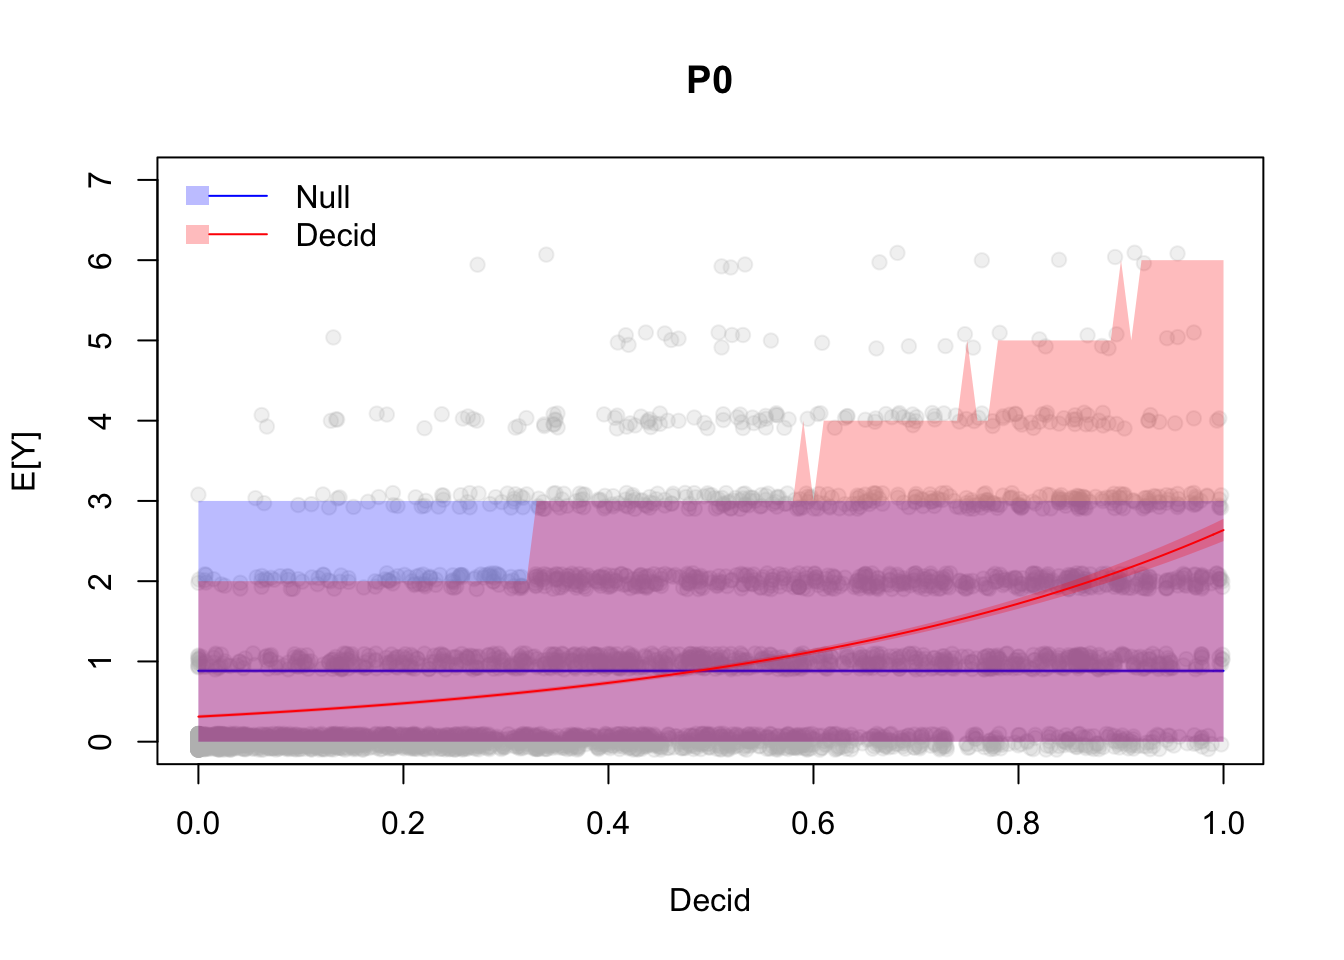
\includegraphics{qpad-book_files/figure-latex/regr-pois_PI-1.pdf}

\BeginKnitrBlock{rmdexercise}
\textbf{Exercise}

What can we conclude from this plot?

Coverage is comparable, so what is the difference then?

Which model should I use for prediction and why? (Hint: look at the non overlapping regions.)
\EndKnitrBlock{rmdexercise}

\hypertarget{additive-model}{%
\section{Additive model}\label{additive-model}}

Generalized additive models (GAMs) are semiparametric, meaning that
parametric assumptions apply, but responses are modelled more flexibly.

\begin{Shaded}
\begin{Highlighting}[]
\NormalTok{mGAM <-}\StringTok{ }\NormalTok{mgcv}\OperatorTok{::}\KeywordTok{gam}\NormalTok{(y }\OperatorTok{~}\StringTok{ }\KeywordTok{s}\NormalTok{(Decid), x, }\DataTypeTok{family=}\NormalTok{poisson)}
\KeywordTok{summary}\NormalTok{(mGAM)}
\end{Highlighting}
\end{Shaded}

\begin{verbatim}
## 
## Family: poisson 
## Link function: log 
## 
## Formula:
## y ~ s(Decid)
## 
## Parametric coefficients:
##             Estimate Std. Error z value Pr(>|z|)    
## (Intercept)  -0.5606     0.0283   -19.8   <2e-16 ***
## ---
## Signif. codes:  0 '***' 0.001 '**' 0.01 '*' 0.05 '.' 0.1 ' ' 1
## 
## Approximate significance of smooth terms:
##           edf Ref.df Chi.sq p-value    
## s(Decid) 8.56   8.94   1193  <2e-16 ***
## ---
## Signif. codes:  0 '***' 0.001 '**' 0.01 '*' 0.05 '.' 0.1 ' ' 1
## 
## R-sq.(adj) =  0.239   Deviance explained =   29%
## UBRE = 0.15808  Scale est. = 1         n = 4569
\end{verbatim}

\begin{Shaded}
\begin{Highlighting}[]
\KeywordTok{plot}\NormalTok{(mGAM)}
\end{Highlighting}
\end{Shaded}

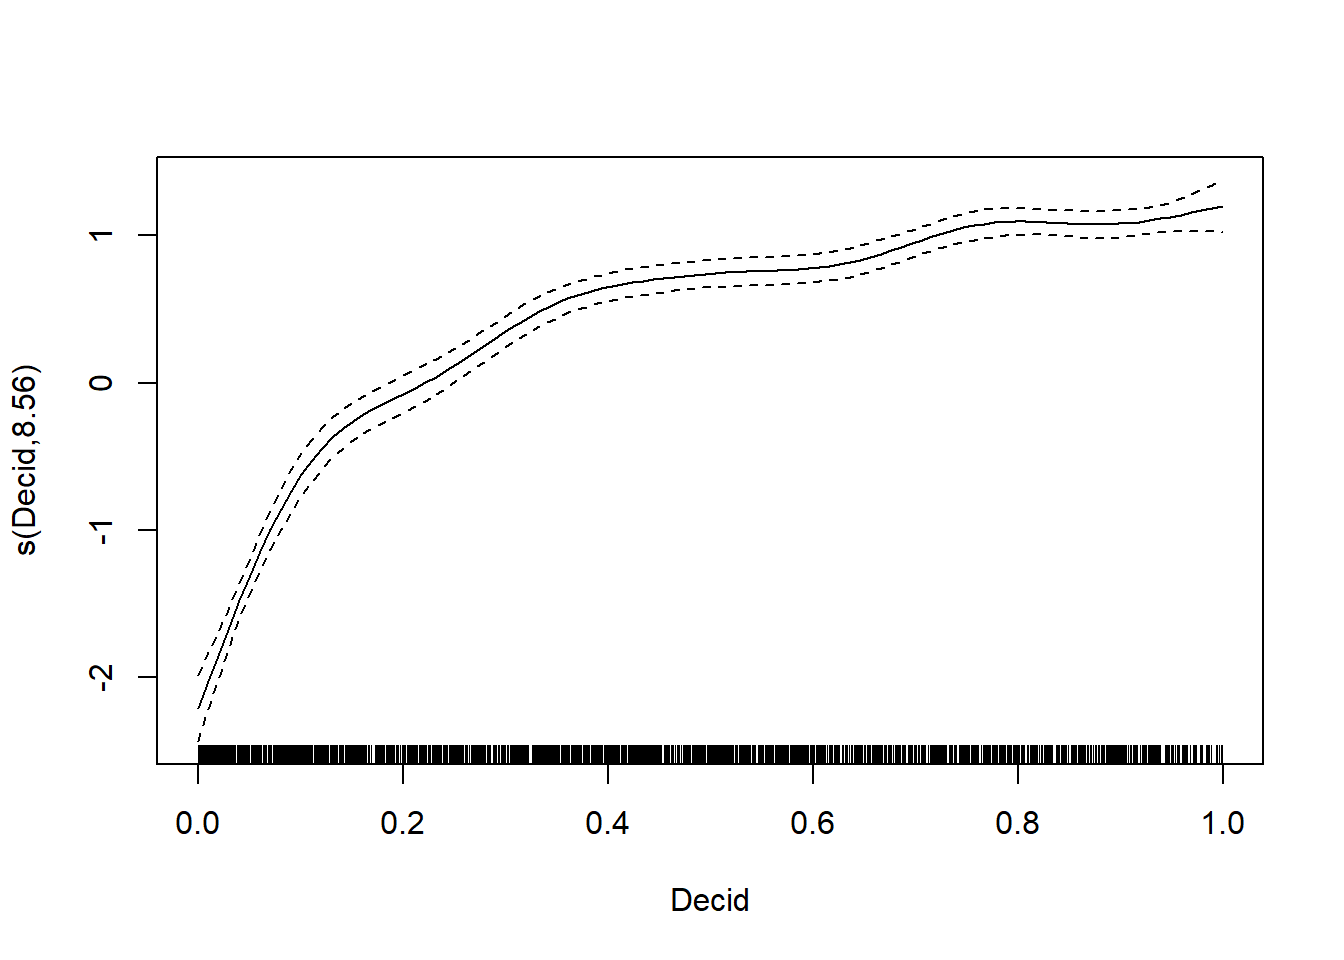
\includegraphics{qpad-book_files/figure-latex/regr-gam-1.pdf}

\begin{Shaded}
\begin{Highlighting}[]
\NormalTok{fitCT <-}\StringTok{ }\KeywordTok{predict}\NormalTok{(mCT, x[}\KeywordTok{order}\NormalTok{(x}\OperatorTok{$}\NormalTok{Decid),])}
\NormalTok{fitGAM <-}\StringTok{ }\KeywordTok{predict}\NormalTok{(mGAM, xnew, }\DataTypeTok{type=}\StringTok{"response"}\NormalTok{)}

\KeywordTok{plot}\NormalTok{(yj }\OperatorTok{~}\StringTok{ }\NormalTok{Decid, x, }\DataTypeTok{xlab=}\StringTok{"Decid"}\NormalTok{, }\DataTypeTok{ylab=}\StringTok{"E[Y]"}\NormalTok{,}
  \DataTypeTok{ylim=}\KeywordTok{c}\NormalTok{(}\DecValTok{0}\NormalTok{, }\KeywordTok{max}\NormalTok{(PI1}\OperatorTok{$}\NormalTok{upr)}\OperatorTok{+}\DecValTok{1}\NormalTok{), }\DataTypeTok{pch=}\DecValTok{19}\NormalTok{, }\DataTypeTok{col=}\StringTok{"#bbbbbb33"}\NormalTok{, }\DataTypeTok{main=}\StringTok{"P0"}\NormalTok{)}
\KeywordTok{lines}\NormalTok{(CI0}\OperatorTok{$}\NormalTok{fit }\OperatorTok{~}\StringTok{ }\NormalTok{xnew}\OperatorTok{$}\NormalTok{Decid, }\DataTypeTok{lty=}\DecValTok{1}\NormalTok{, }\DataTypeTok{col=}\DecValTok{1}\NormalTok{)}
\KeywordTok{lines}\NormalTok{(CI1}\OperatorTok{$}\NormalTok{fit }\OperatorTok{~}\StringTok{ }\NormalTok{xnew}\OperatorTok{$}\NormalTok{Decid, }\DataTypeTok{lty=}\DecValTok{1}\NormalTok{, }\DataTypeTok{col=}\DecValTok{2}\NormalTok{)}
\KeywordTok{lines}\NormalTok{(fitCT }\OperatorTok{~}\StringTok{ }\NormalTok{x}\OperatorTok{$}\NormalTok{Decid[}\KeywordTok{order}\NormalTok{(x}\OperatorTok{$}\NormalTok{Decid)], }\DataTypeTok{lty=}\DecValTok{1}\NormalTok{, }\DataTypeTok{col=}\DecValTok{3}\NormalTok{)}
\KeywordTok{lines}\NormalTok{(fitGAM }\OperatorTok{~}\StringTok{ }\NormalTok{xnew}\OperatorTok{$}\NormalTok{Decid, }\DataTypeTok{lty=}\DecValTok{1}\NormalTok{, }\DataTypeTok{col=}\DecValTok{4}\NormalTok{)}
\KeywordTok{legend}\NormalTok{(}\StringTok{"topleft"}\NormalTok{, }\DataTypeTok{bty=}\StringTok{"n"}\NormalTok{, }\DataTypeTok{lty=}\DecValTok{1}\NormalTok{, }\DataTypeTok{col=}\DecValTok{1}\OperatorTok{:}\DecValTok{4}\NormalTok{,}
  \DataTypeTok{legend=}\KeywordTok{c}\NormalTok{(}\StringTok{"Null"}\NormalTok{, }\StringTok{"Decid"}\NormalTok{, }\StringTok{"ctree"}\NormalTok{, }\StringTok{"GAM"}\NormalTok{))}
\end{Highlighting}
\end{Shaded}

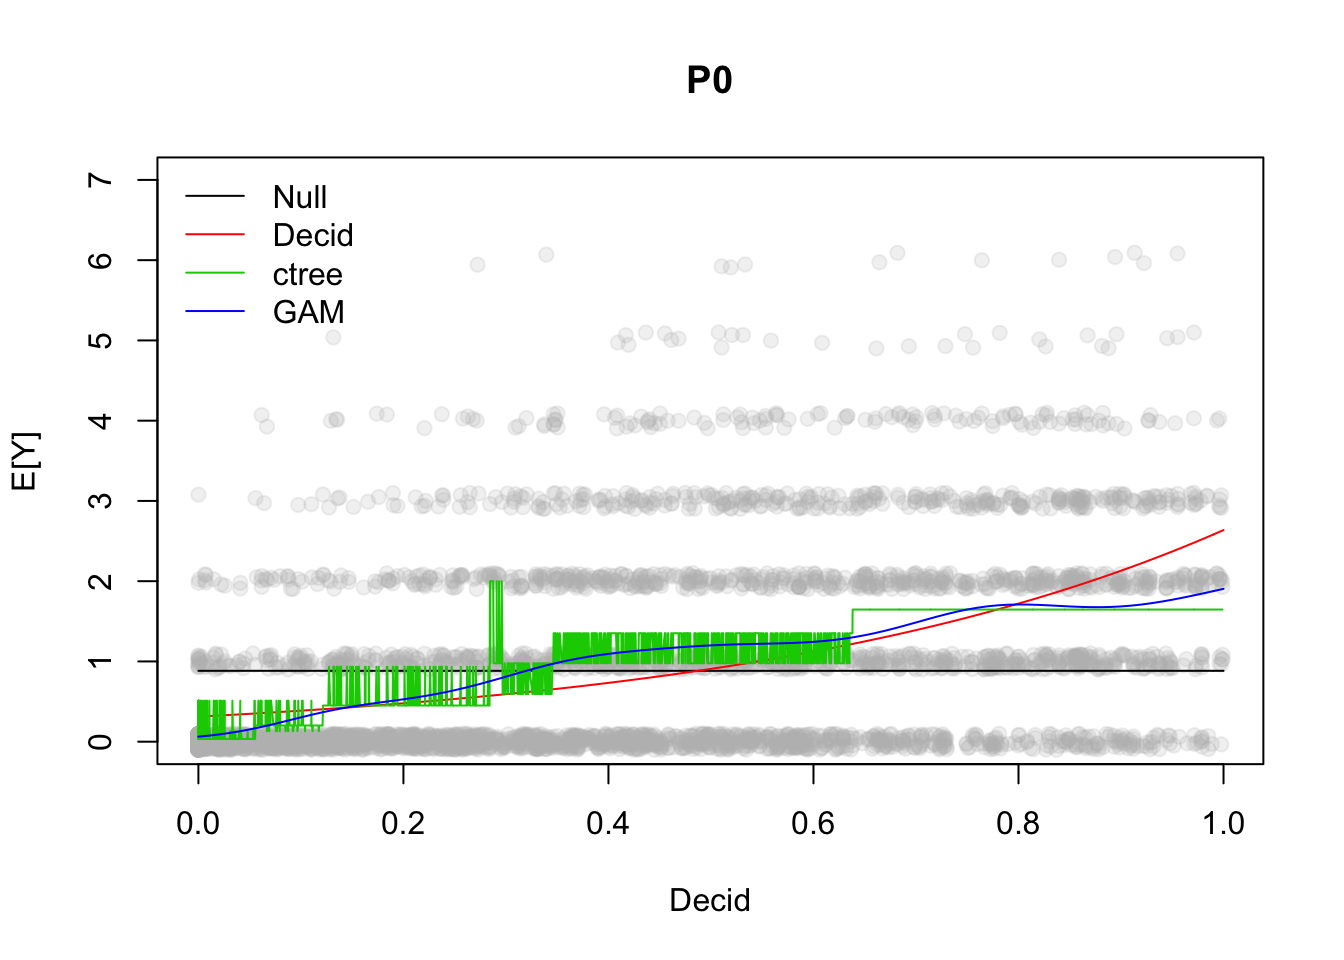
\includegraphics{qpad-book_files/figure-latex/regr-glm_plots-1.pdf}

\BeginKnitrBlock{rmdexercise}
\textbf{Exercise}

Play with GAM and other variables to understand response curves:

\texttt{plot(mgcv::gam(y\ \textasciitilde{}\ s(\textless{}variable\_name\textgreater{}),\ data=x,\ family=poisson))}
\EndKnitrBlock{rmdexercise}

\hypertarget{nonlinear-terms}{%
\section{Nonlinear terms}\label{nonlinear-terms}}

We can use polynomial terms to approximate the GAM fit:

\begin{Shaded}
\begin{Highlighting}[]
\NormalTok{mP12 <-}\StringTok{ }\KeywordTok{glm}\NormalTok{(y }\OperatorTok{~}\StringTok{ }\NormalTok{Decid }\OperatorTok{+}\StringTok{ }\KeywordTok{I}\NormalTok{(Decid}\OperatorTok{^}\DecValTok{2}\NormalTok{), }\DataTypeTok{data=}\NormalTok{x, }\DataTypeTok{family=}\NormalTok{poisson)}
\NormalTok{mP13 <-}\StringTok{ }\KeywordTok{glm}\NormalTok{(y }\OperatorTok{~}\StringTok{ }\NormalTok{Decid }\OperatorTok{+}\StringTok{ }\KeywordTok{I}\NormalTok{(Decid}\OperatorTok{^}\DecValTok{2}\NormalTok{) }\OperatorTok{+}\StringTok{ }\KeywordTok{I}\NormalTok{(Decid}\OperatorTok{^}\DecValTok{3}\NormalTok{), }\DataTypeTok{data=}\NormalTok{x, }\DataTypeTok{family=}\NormalTok{poisson)}
\NormalTok{mP14 <-}\StringTok{ }\KeywordTok{glm}\NormalTok{(y }\OperatorTok{~}\StringTok{ }\NormalTok{Decid }\OperatorTok{+}\StringTok{ }\KeywordTok{I}\NormalTok{(Decid}\OperatorTok{^}\DecValTok{2}\NormalTok{) }\OperatorTok{+}\StringTok{ }\KeywordTok{I}\NormalTok{(Decid}\OperatorTok{^}\DecValTok{3}\NormalTok{) }\OperatorTok{+}\StringTok{ }\KeywordTok{I}\NormalTok{(Decid}\OperatorTok{^}\DecValTok{4}\NormalTok{), }\DataTypeTok{data=}\NormalTok{x, }\DataTypeTok{family=}\NormalTok{poisson)}
\KeywordTok{model.sel}\NormalTok{(mP1, mP12, mP13, mP14, mGAM)}
\end{Highlighting}
\end{Shaded}

\begin{verbatim}
## Model selection table 
##        (Int)    Dcd  Dcd^2  Dcd^3  Dcd^4 s(Dcd) class df logLik  AICc
## mGAM -0.5606                                  +   gam  9  -5209 10438
## mP14 -2.6640 16.640 -38.60 41.470 -16.31          glm  5  -5215 10441
## mP13 -2.3910 11.400 -16.31  8.066                 glm  4  -5226 10461
## mP12 -1.9240  6.259  -3.97                        glm  3  -5269 10544
## mP1  -1.1640  2.134                               glm  2  -5442 10887
##       delta weight
## mGAM   0.00   0.84
## mP14   3.31   0.16
## mP13  23.42   0.00
## mP12 106.04   0.00
## mP1  449.60   0.00
## Models ranked by AICc(x)
\end{verbatim}

Not a surprise that the most complex model won. GAM was more complex than that.

\begin{Shaded}
\begin{Highlighting}[]
\NormalTok{pr <-}\StringTok{ }\KeywordTok{cbind}\NormalTok{(}
  \KeywordTok{predict}\NormalTok{(mP1, xnew, }\DataTypeTok{type=}\StringTok{"response"}\NormalTok{),}
  \KeywordTok{predict}\NormalTok{(mP12, xnew, }\DataTypeTok{type=}\StringTok{"response"}\NormalTok{),}
  \KeywordTok{predict}\NormalTok{(mP13, xnew, }\DataTypeTok{type=}\StringTok{"response"}\NormalTok{),}
  \KeywordTok{predict}\NormalTok{(mP14, xnew, }\DataTypeTok{type=}\StringTok{"response"}\NormalTok{),}
\NormalTok{  fitGAM)}
\KeywordTok{matplot}\NormalTok{(xnew}\OperatorTok{$}\NormalTok{Decid, pr, }\DataTypeTok{lty=}\DecValTok{1}\NormalTok{, }\DataTypeTok{type=}\StringTok{"l"}\NormalTok{,}
  \DataTypeTok{xlab=}\StringTok{"Decid"}\NormalTok{, }\DataTypeTok{ylab=}\StringTok{"E[Y]"}\NormalTok{)}
\KeywordTok{legend}\NormalTok{(}\StringTok{"topleft"}\NormalTok{, }\DataTypeTok{lty=}\DecValTok{1}\NormalTok{, }\DataTypeTok{col=}\DecValTok{1}\OperatorTok{:}\DecValTok{5}\NormalTok{, }\DataTypeTok{bty=}\StringTok{"n"}\NormalTok{,}
  \DataTypeTok{legend=}\KeywordTok{c}\NormalTok{(}\StringTok{"Linear"}\NormalTok{, }\StringTok{"Quadratic"}\NormalTok{, }\StringTok{"Cubic"}\NormalTok{, }\StringTok{"Quartic"}\NormalTok{, }\StringTok{"GAM"}\NormalTok{))}
\end{Highlighting}
\end{Shaded}

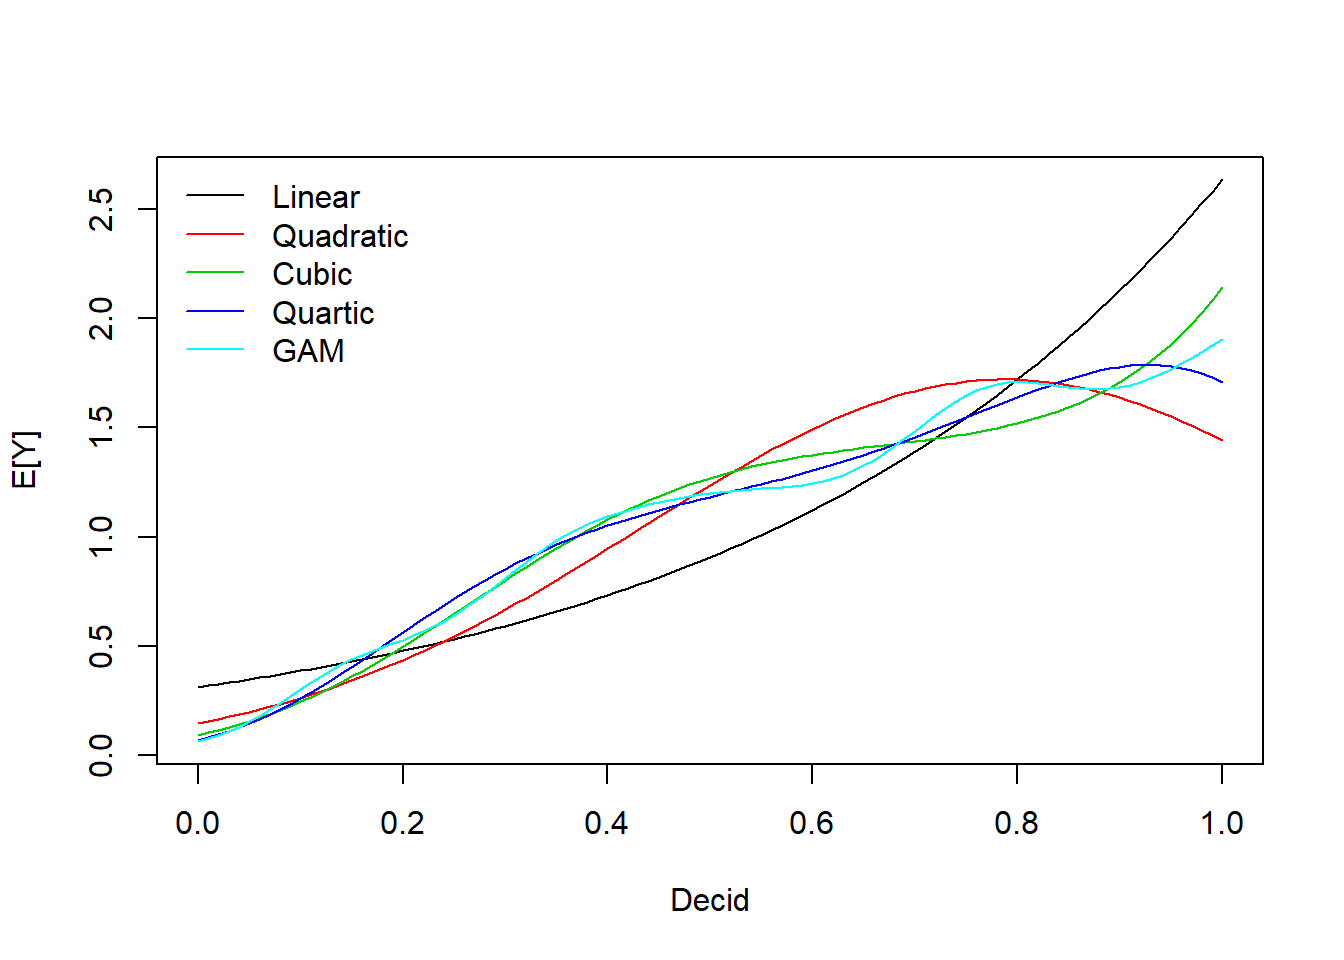
\includegraphics{qpad-book_files/figure-latex/regr-pois_poly_plot-1.pdf}

Let's see how these affect our prediction intervals:

\begin{Shaded}
\begin{Highlighting}[]
\NormalTok{CI12 <-}\StringTok{ }\KeywordTok{predict_sim}\NormalTok{(mP12, xnew, }\DataTypeTok{interval=}\StringTok{"confidence"}\NormalTok{, }\DataTypeTok{level=}\DecValTok{1}\OperatorTok{-}\NormalTok{alpha, }\DataTypeTok{B=}\NormalTok{B)}
\NormalTok{PI12 <-}\StringTok{ }\KeywordTok{predict_sim}\NormalTok{(mP12, xnew, }\DataTypeTok{interval=}\StringTok{"prediction"}\NormalTok{, }\DataTypeTok{level=}\DecValTok{1}\OperatorTok{-}\NormalTok{alpha, }\DataTypeTok{B=}\NormalTok{B)}
\NormalTok{CI13 <-}\StringTok{ }\KeywordTok{predict_sim}\NormalTok{(mP13, xnew, }\DataTypeTok{interval=}\StringTok{"confidence"}\NormalTok{, }\DataTypeTok{level=}\DecValTok{1}\OperatorTok{-}\NormalTok{alpha, }\DataTypeTok{B=}\NormalTok{B)}
\NormalTok{PI13 <-}\StringTok{ }\KeywordTok{predict_sim}\NormalTok{(mP13, xnew, }\DataTypeTok{interval=}\StringTok{"prediction"}\NormalTok{, }\DataTypeTok{level=}\DecValTok{1}\OperatorTok{-}\NormalTok{alpha, }\DataTypeTok{B=}\NormalTok{B)}
\NormalTok{CI14 <-}\StringTok{ }\KeywordTok{predict_sim}\NormalTok{(mP14, xnew, }\DataTypeTok{interval=}\StringTok{"confidence"}\NormalTok{, }\DataTypeTok{level=}\DecValTok{1}\OperatorTok{-}\NormalTok{alpha, }\DataTypeTok{B=}\NormalTok{B)}
\NormalTok{PI14 <-}\StringTok{ }\KeywordTok{predict_sim}\NormalTok{(mP14, xnew, }\DataTypeTok{interval=}\StringTok{"prediction"}\NormalTok{, }\DataTypeTok{level=}\DecValTok{1}\OperatorTok{-}\NormalTok{alpha, }\DataTypeTok{B=}\NormalTok{B)}

\NormalTok{op <-}\StringTok{ }\KeywordTok{par}\NormalTok{(}\DataTypeTok{mfrow=}\KeywordTok{c}\NormalTok{(}\DecValTok{2}\NormalTok{,}\DecValTok{2}\NormalTok{))}
\KeywordTok{plot}\NormalTok{(yj }\OperatorTok{~}\StringTok{ }\NormalTok{Decid, x, }\DataTypeTok{xlab=}\StringTok{"Decid"}\NormalTok{, }\DataTypeTok{ylab=}\StringTok{"E[Y]"}\NormalTok{,}
  \DataTypeTok{ylim=}\KeywordTok{c}\NormalTok{(}\DecValTok{0}\NormalTok{, }\KeywordTok{max}\NormalTok{(PI1}\OperatorTok{$}\NormalTok{upr)}\OperatorTok{+}\DecValTok{1}\NormalTok{), }\DataTypeTok{pch=}\DecValTok{19}\NormalTok{, }\DataTypeTok{col=}\StringTok{"#bbbbbb33"}\NormalTok{, }\DataTypeTok{main=}\StringTok{"Linear"}\NormalTok{)}
\KeywordTok{polygon}\NormalTok{(}\KeywordTok{c}\NormalTok{(xnew}\OperatorTok{$}\NormalTok{Decid, }\KeywordTok{rev}\NormalTok{(xnew}\OperatorTok{$}\NormalTok{Decid)),}
  \KeywordTok{c}\NormalTok{(PI1}\OperatorTok{$}\NormalTok{lwr, }\KeywordTok{rev}\NormalTok{(PI1}\OperatorTok{$}\NormalTok{upr)), }\DataTypeTok{border=}\OtherTok{NA}\NormalTok{, }\DataTypeTok{col=}\StringTok{"#0000ff44"}\NormalTok{)}
\KeywordTok{polygon}\NormalTok{(}\KeywordTok{c}\NormalTok{(xnew}\OperatorTok{$}\NormalTok{Decid, }\KeywordTok{rev}\NormalTok{(xnew}\OperatorTok{$}\NormalTok{Decid)),}
  \KeywordTok{c}\NormalTok{(CI1}\OperatorTok{$}\NormalTok{lwr, }\KeywordTok{rev}\NormalTok{(CI1}\OperatorTok{$}\NormalTok{upr)), }\DataTypeTok{border=}\OtherTok{NA}\NormalTok{, }\DataTypeTok{col=}\StringTok{"#0000ff88"}\NormalTok{)}
\KeywordTok{lines}\NormalTok{(CI1}\OperatorTok{$}\NormalTok{fit }\OperatorTok{~}\StringTok{ }\NormalTok{xnew}\OperatorTok{$}\NormalTok{Decid, }\DataTypeTok{lty=}\DecValTok{1}\NormalTok{, }\DataTypeTok{col=}\DecValTok{4}\NormalTok{)}
\KeywordTok{lines}\NormalTok{(fitGAM }\OperatorTok{~}\StringTok{ }\NormalTok{xnew}\OperatorTok{$}\NormalTok{Decid, }\DataTypeTok{lty=}\DecValTok{2}\NormalTok{, }\DataTypeTok{col=}\DecValTok{1}\NormalTok{)}

\KeywordTok{plot}\NormalTok{(yj }\OperatorTok{~}\StringTok{ }\NormalTok{Decid, x, }\DataTypeTok{xlab=}\StringTok{"Decid"}\NormalTok{, }\DataTypeTok{ylab=}\StringTok{"E[Y]"}\NormalTok{,}
  \DataTypeTok{ylim=}\KeywordTok{c}\NormalTok{(}\DecValTok{0}\NormalTok{, }\KeywordTok{max}\NormalTok{(PI1}\OperatorTok{$}\NormalTok{upr)}\OperatorTok{+}\DecValTok{1}\NormalTok{), }\DataTypeTok{pch=}\DecValTok{19}\NormalTok{, }\DataTypeTok{col=}\StringTok{"#bbbbbb33"}\NormalTok{, }\DataTypeTok{main=}\StringTok{"Quadratic"}\NormalTok{)}
\KeywordTok{polygon}\NormalTok{(}\KeywordTok{c}\NormalTok{(xnew}\OperatorTok{$}\NormalTok{Decid, }\KeywordTok{rev}\NormalTok{(xnew}\OperatorTok{$}\NormalTok{Decid)),}
  \KeywordTok{c}\NormalTok{(PI12}\OperatorTok{$}\NormalTok{lwr, }\KeywordTok{rev}\NormalTok{(PI12}\OperatorTok{$}\NormalTok{upr)), }\DataTypeTok{border=}\OtherTok{NA}\NormalTok{, }\DataTypeTok{col=}\StringTok{"#0000ff44"}\NormalTok{)}
\KeywordTok{polygon}\NormalTok{(}\KeywordTok{c}\NormalTok{(xnew}\OperatorTok{$}\NormalTok{Decid, }\KeywordTok{rev}\NormalTok{(xnew}\OperatorTok{$}\NormalTok{Decid)),}
  \KeywordTok{c}\NormalTok{(CI12}\OperatorTok{$}\NormalTok{lwr, }\KeywordTok{rev}\NormalTok{(CI12}\OperatorTok{$}\NormalTok{upr)), }\DataTypeTok{border=}\OtherTok{NA}\NormalTok{, }\DataTypeTok{col=}\StringTok{"#0000ff88"}\NormalTok{)}
\KeywordTok{lines}\NormalTok{(CI12}\OperatorTok{$}\NormalTok{fit }\OperatorTok{~}\StringTok{ }\NormalTok{xnew}\OperatorTok{$}\NormalTok{Decid, }\DataTypeTok{lty=}\DecValTok{1}\NormalTok{, }\DataTypeTok{col=}\DecValTok{4}\NormalTok{)}
\KeywordTok{lines}\NormalTok{(fitGAM }\OperatorTok{~}\StringTok{ }\NormalTok{xnew}\OperatorTok{$}\NormalTok{Decid, }\DataTypeTok{lty=}\DecValTok{2}\NormalTok{, }\DataTypeTok{col=}\DecValTok{1}\NormalTok{)}

\KeywordTok{plot}\NormalTok{(yj }\OperatorTok{~}\StringTok{ }\NormalTok{Decid, x, }\DataTypeTok{xlab=}\StringTok{"Decid"}\NormalTok{, }\DataTypeTok{ylab=}\StringTok{"E[Y]"}\NormalTok{,}
  \DataTypeTok{ylim=}\KeywordTok{c}\NormalTok{(}\DecValTok{0}\NormalTok{, }\KeywordTok{max}\NormalTok{(PI1}\OperatorTok{$}\NormalTok{upr)}\OperatorTok{+}\DecValTok{1}\NormalTok{), }\DataTypeTok{pch=}\DecValTok{19}\NormalTok{, }\DataTypeTok{col=}\StringTok{"#bbbbbb33"}\NormalTok{, }\DataTypeTok{main=}\StringTok{"P0"}\NormalTok{)}
\KeywordTok{polygon}\NormalTok{(}\KeywordTok{c}\NormalTok{(xnew}\OperatorTok{$}\NormalTok{Decid, }\KeywordTok{rev}\NormalTok{(xnew}\OperatorTok{$}\NormalTok{Decid)),}
  \KeywordTok{c}\NormalTok{(PI13}\OperatorTok{$}\NormalTok{lwr, }\KeywordTok{rev}\NormalTok{(PI13}\OperatorTok{$}\NormalTok{upr)), }\DataTypeTok{border=}\OtherTok{NA}\NormalTok{, }\DataTypeTok{col=}\StringTok{"#0000ff44"}\NormalTok{)}
\KeywordTok{polygon}\NormalTok{(}\KeywordTok{c}\NormalTok{(xnew}\OperatorTok{$}\NormalTok{Decid, }\KeywordTok{rev}\NormalTok{(xnew}\OperatorTok{$}\NormalTok{Decid)),}
  \KeywordTok{c}\NormalTok{(CI13}\OperatorTok{$}\NormalTok{lwr, }\KeywordTok{rev}\NormalTok{(CI13}\OperatorTok{$}\NormalTok{upr)), }\DataTypeTok{border=}\OtherTok{NA}\NormalTok{, }\DataTypeTok{col=}\StringTok{"#0000ff88"}\NormalTok{)}
\KeywordTok{lines}\NormalTok{(CI13}\OperatorTok{$}\NormalTok{fit }\OperatorTok{~}\StringTok{ }\NormalTok{xnew}\OperatorTok{$}\NormalTok{Decid, }\DataTypeTok{lty=}\DecValTok{1}\NormalTok{, }\DataTypeTok{col=}\DecValTok{4}\NormalTok{)}
\KeywordTok{lines}\NormalTok{(fitGAM }\OperatorTok{~}\StringTok{ }\NormalTok{xnew}\OperatorTok{$}\NormalTok{Decid, }\DataTypeTok{lty=}\DecValTok{2}\NormalTok{, }\DataTypeTok{col=}\DecValTok{1}\NormalTok{)}

\KeywordTok{plot}\NormalTok{(yj }\OperatorTok{~}\StringTok{ }\NormalTok{Decid, x, }\DataTypeTok{xlab=}\StringTok{"Decid"}\NormalTok{, }\DataTypeTok{ylab=}\StringTok{"E[Y]"}\NormalTok{,}
  \DataTypeTok{ylim=}\KeywordTok{c}\NormalTok{(}\DecValTok{0}\NormalTok{, }\KeywordTok{max}\NormalTok{(PI1}\OperatorTok{$}\NormalTok{upr)}\OperatorTok{+}\DecValTok{1}\NormalTok{), }\DataTypeTok{pch=}\DecValTok{19}\NormalTok{, }\DataTypeTok{col=}\StringTok{"#bbbbbb33"}\NormalTok{, }\DataTypeTok{main=}\StringTok{"P0"}\NormalTok{)}
\KeywordTok{polygon}\NormalTok{(}\KeywordTok{c}\NormalTok{(xnew}\OperatorTok{$}\NormalTok{Decid, }\KeywordTok{rev}\NormalTok{(xnew}\OperatorTok{$}\NormalTok{Decid)),}
  \KeywordTok{c}\NormalTok{(PI14}\OperatorTok{$}\NormalTok{lwr, }\KeywordTok{rev}\NormalTok{(PI14}\OperatorTok{$}\NormalTok{upr)), }\DataTypeTok{border=}\OtherTok{NA}\NormalTok{, }\DataTypeTok{col=}\StringTok{"#0000ff44"}\NormalTok{)}
\KeywordTok{polygon}\NormalTok{(}\KeywordTok{c}\NormalTok{(xnew}\OperatorTok{$}\NormalTok{Decid, }\KeywordTok{rev}\NormalTok{(xnew}\OperatorTok{$}\NormalTok{Decid)),}
  \KeywordTok{c}\NormalTok{(CI14}\OperatorTok{$}\NormalTok{lwr, }\KeywordTok{rev}\NormalTok{(CI14}\OperatorTok{$}\NormalTok{upr)), }\DataTypeTok{border=}\OtherTok{NA}\NormalTok{, }\DataTypeTok{col=}\StringTok{"#0000ff88"}\NormalTok{)}
\KeywordTok{lines}\NormalTok{(CI14}\OperatorTok{$}\NormalTok{fit }\OperatorTok{~}\StringTok{ }\NormalTok{xnew}\OperatorTok{$}\NormalTok{Decid, }\DataTypeTok{lty=}\DecValTok{1}\NormalTok{, }\DataTypeTok{col=}\DecValTok{4}\NormalTok{)}
\KeywordTok{lines}\NormalTok{(fitGAM }\OperatorTok{~}\StringTok{ }\NormalTok{xnew}\OperatorTok{$}\NormalTok{Decid, }\DataTypeTok{lty=}\DecValTok{2}\NormalTok{, }\DataTypeTok{col=}\DecValTok{1}\NormalTok{)}
\end{Highlighting}
\end{Shaded}

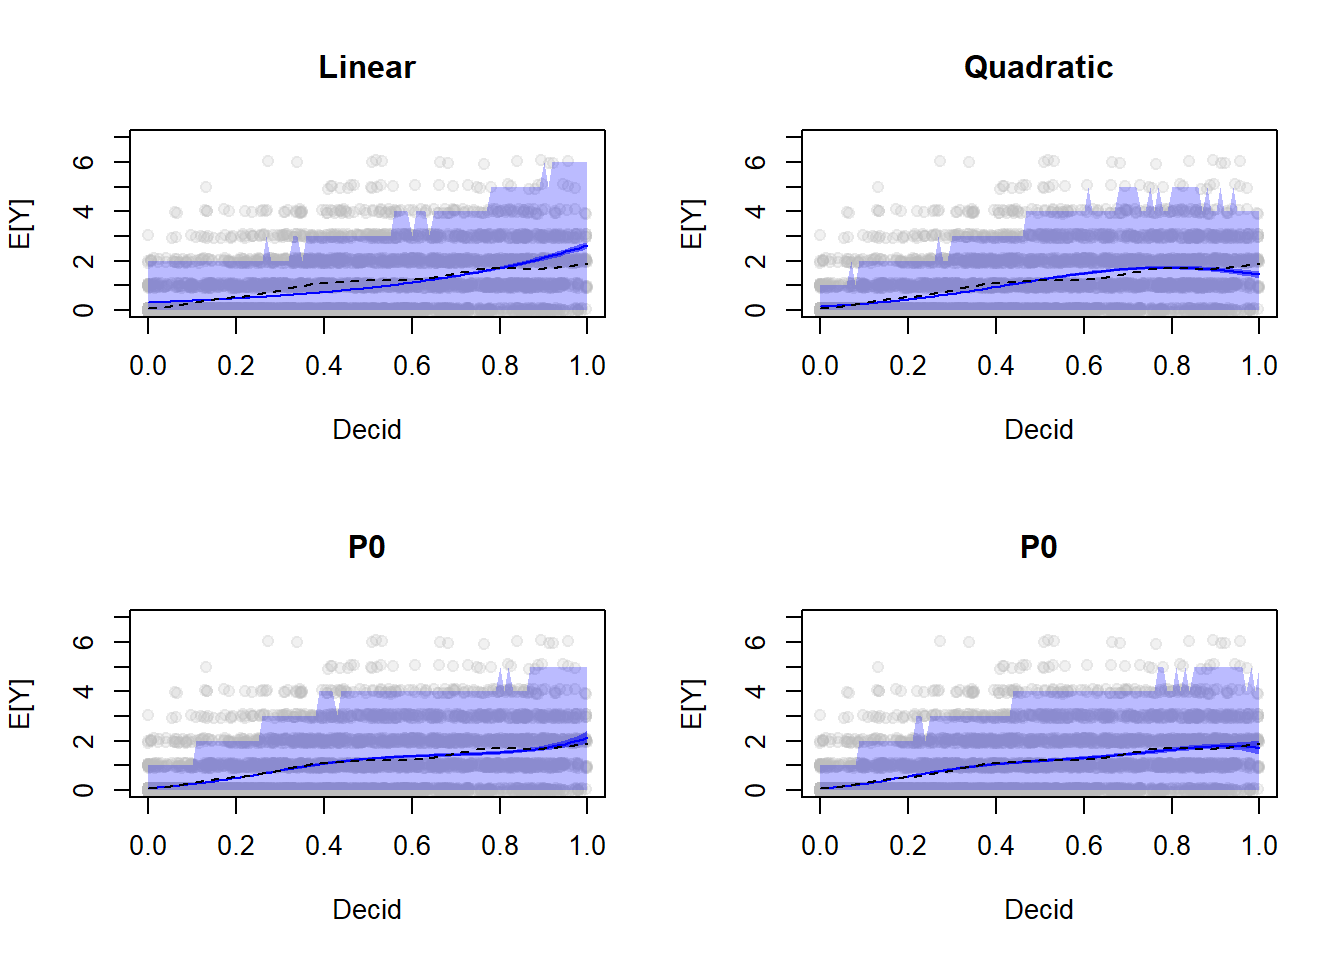
\includegraphics{qpad-book_files/figure-latex/regr-pois_poly_pi-1.pdf}

\begin{Shaded}
\begin{Highlighting}[]
\KeywordTok{par}\NormalTok{(op)}
\end{Highlighting}
\end{Shaded}

\hypertarget{categorical-variables}{%
\section{Categorical variables}\label{categorical-variables}}

Categorical variables are expanded into a \emph{model matrix} before estimation.
The model matrix usually contains indicator variables for each level
(value 1 when factor value equals a particular label, 0 otherwise)
except for the \emph{reference category}
(check \texttt{relevel} if you want to change the reference category).

The estimate for the reference category comes from the intercept,
the rest of the estimates are relative to the reference category.
In the log-linear model example this means a ratio.

\begin{Shaded}
\begin{Highlighting}[]
\KeywordTok{head}\NormalTok{(}\KeywordTok{model.matrix}\NormalTok{(}\OperatorTok{~}\NormalTok{DEC, x))}
\end{Highlighting}
\end{Shaded}

\begin{verbatim}
##         (Intercept) DEC
## CL10102           1   1
## CL10106           1   0
## CL10108           1   0
## CL10109           1   1
## CL10111           1   1
## CL10112           1   1
\end{verbatim}

\begin{Shaded}
\begin{Highlighting}[]
\NormalTok{mP2 <-}\StringTok{ }\KeywordTok{glm}\NormalTok{(y }\OperatorTok{~}\StringTok{ }\NormalTok{DEC, }\DataTypeTok{data=}\NormalTok{x, }\DataTypeTok{family=}\NormalTok{poisson)}
\KeywordTok{summary}\NormalTok{(mP2)}
\end{Highlighting}
\end{Shaded}

\begin{verbatim}
## 
## Call:
## glm(formula = y ~ DEC, family = poisson, data = x)
## 
## Deviance Residuals: 
##    Min      1Q  Median      3Q     Max  
## -1.691  -0.921  -0.921   0.449   4.543  
## 
## Coefficients:
##             Estimate Std. Error z value Pr(>|z|)    
## (Intercept)  -0.8577     0.0308   -27.8   <2e-16 ***
## DEC           1.2156     0.0358    33.9   <2e-16 ***
## ---
## Signif. codes:  0 '***' 0.001 '**' 0.01 '*' 0.05 '.' 0.1 ' ' 1
## 
## (Dispersion parameter for poisson family taken to be 1)
## 
##     Null deviance: 7424.8  on 4568  degrees of freedom
## Residual deviance: 6095.5  on 4567  degrees of freedom
## AIC: 11246
## 
## Number of Fisher Scoring iterations: 6
\end{verbatim}

\begin{Shaded}
\begin{Highlighting}[]
\KeywordTok{coef}\NormalTok{(mP2)}
\end{Highlighting}
\end{Shaded}

\begin{verbatim}
## (Intercept)         DEC 
##     -0.8577      1.2156
\end{verbatim}

The estimate for a non-deciduous landscape is
\(e^{\beta_0}\), and it is \(e^{\beta_0}e^{\beta_1}\) for deciduous landscapes.
Of course such binary classification at the landscape (1 km\(^2\)) level
doesn't really makes sense for various reasons:

\begin{Shaded}
\begin{Highlighting}[]
\KeywordTok{boxplot}\NormalTok{(Decid }\OperatorTok{~}\StringTok{ }\NormalTok{DEC, x)}
\end{Highlighting}
\end{Shaded}

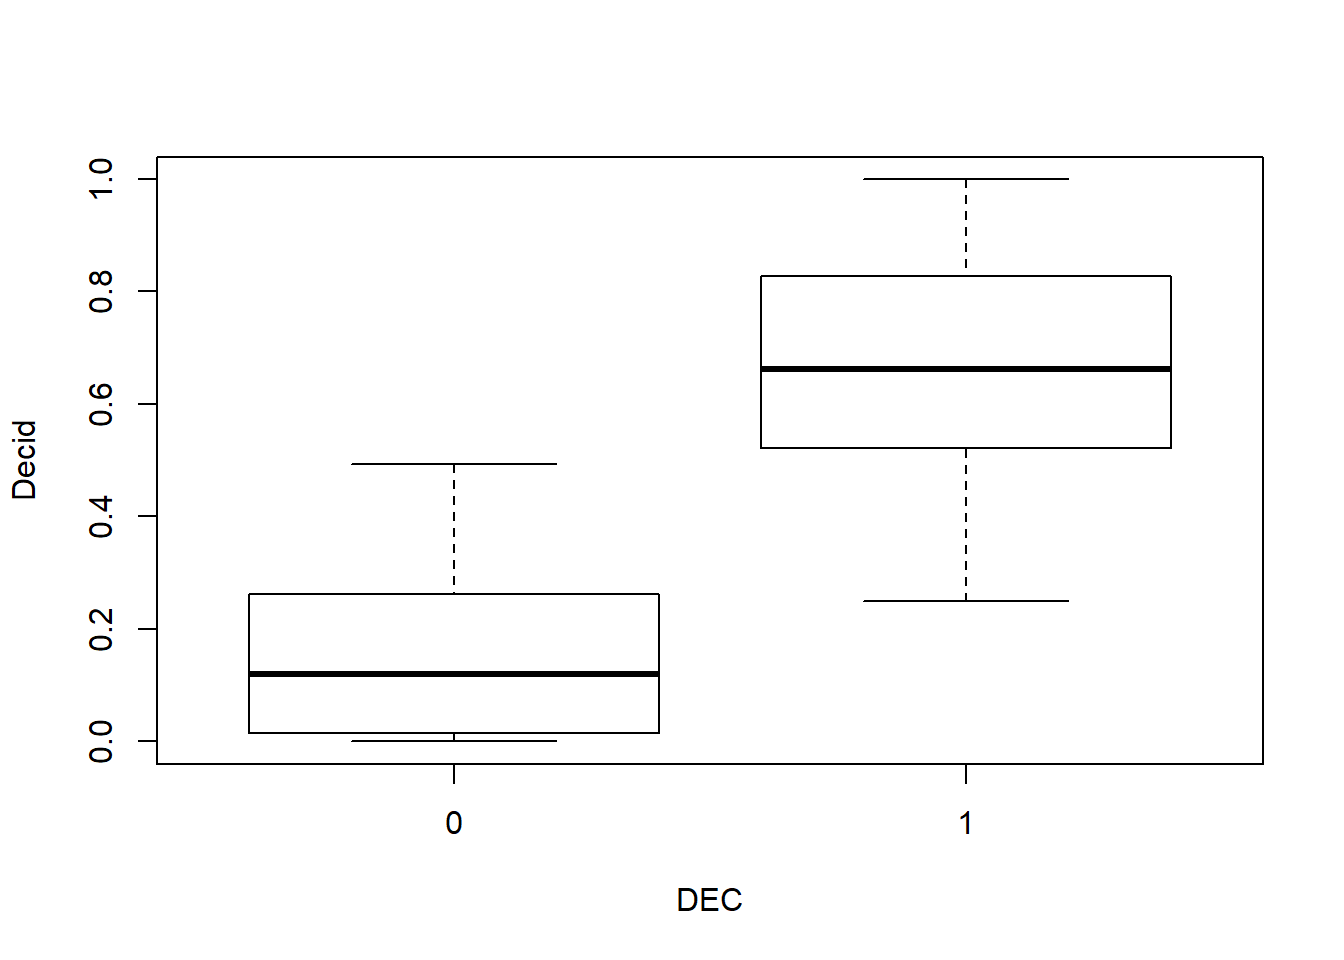
\includegraphics{qpad-book_files/figure-latex/regr-pois_cat1-1.pdf}

\begin{Shaded}
\begin{Highlighting}[]
\KeywordTok{model.sel}\NormalTok{(mP1, mP2)}
\end{Highlighting}
\end{Shaded}

\begin{verbatim}
## Model selection table 
##     (Intrc) Decid   DEC df logLik  AICc delta weight
## mP1 -1.1640 2.134        2  -5442 10887   0.0      1
## mP2 -0.8577       1.216  2  -5621 11246 358.6      0
## Models ranked by AICc(x)
\end{verbatim}

\begin{Shaded}
\begin{Highlighting}[]
\KeywordTok{R2dev}\NormalTok{(mP1, mP2)}
\end{Highlighting}
\end{Shaded}

\begin{verbatim}
##          R2   R2adj Deviance    Dev0    DevR     df0     dfR p_value    
## mP1    0.23    0.23  1687.87 7424.78 5736.91 4568.00 4567.00  <2e-16 ***
## mP2    0.18    0.18  1329.23 7424.78 6095.55 4568.00 4567.00  <2e-16 ***
## ---
## Signif. codes:  0 '***' 0.001 '**' 0.01 '*' 0.05 '.' 0.1 ' ' 1
\end{verbatim}

Having estimates for each land cover type improves the model,
but the model using continuous variable is still better

\begin{Shaded}
\begin{Highlighting}[]
\NormalTok{mP3 <-}\StringTok{ }\KeywordTok{glm}\NormalTok{(y }\OperatorTok{~}\StringTok{ }\NormalTok{HAB, }\DataTypeTok{data=}\NormalTok{x, }\DataTypeTok{family=}\NormalTok{poisson)}
\KeywordTok{summary}\NormalTok{(mP3)}
\end{Highlighting}
\end{Shaded}

\begin{verbatim}
## 
## Call:
## glm(formula = y ~ HAB, family = poisson, data = x)
## 
## Deviance Residuals: 
##    Min      1Q  Median      3Q     Max  
## -1.691  -0.873  -0.817   0.449   4.832  
## 
## Coefficients:
##             Estimate Std. Error z value Pr(>|z|)   
## (Intercept)   -1.386      0.577   -2.40   0.0163 * 
## HABWater       1.030      0.690    1.49   0.1357   
## HABAgr         0.693      0.913    0.76   0.4477   
## HABUrbInd      0.134      0.764    0.17   0.8612   
## HABRoads     -10.916    201.285   -0.05   0.9567   
## HABDecid       1.744      0.578    3.02   0.0025 **
## HABOpenWet     0.422      0.591    0.71   0.4755   
## HABConif       0.913      0.579    1.58   0.1150   
## HABConifWet    0.288      0.579    0.50   0.6185   
## ---
## Signif. codes:  0 '***' 0.001 '**' 0.01 '*' 0.05 '.' 0.1 ' ' 1
## 
## (Dispersion parameter for poisson family taken to be 1)
## 
##     Null deviance: 7424.8  on 4568  degrees of freedom
## Residual deviance: 5997.2  on 4560  degrees of freedom
## AIC: 11161
## 
## Number of Fisher Scoring iterations: 10
\end{verbatim}

\begin{Shaded}
\begin{Highlighting}[]
\KeywordTok{model.sel}\NormalTok{(mP1, mP2, mP3)}
\end{Highlighting}
\end{Shaded}

\begin{verbatim}
## Model selection table 
##     (Intrc) Decid   DEC HAB df logLik  AICc delta weight
## mP1 -1.1640 2.134            2  -5442 10887   0.0      1
## mP3 -1.3860               +  9  -5572 11162 274.4      0
## mP2 -0.8577       1.216      2  -5621 11246 358.6      0
## Models ranked by AICc(x)
\end{verbatim}

\begin{Shaded}
\begin{Highlighting}[]
\KeywordTok{R2dev}\NormalTok{(mP1, mP2, mP3)}
\end{Highlighting}
\end{Shaded}

\begin{verbatim}
##          R2   R2adj Deviance    Dev0    DevR     df0     dfR p_value    
## mP1    0.23    0.23  1687.87 7424.78 5736.91 4568.00 4567.00  <2e-16 ***
## mP2    0.18    0.18  1329.23 7424.78 6095.55 4568.00 4567.00  <2e-16 ***
## mP3    0.19    0.19  1427.55 7424.78 5997.23 4568.00 4560.00  <2e-16 ***
## ---
## Signif. codes:  0 '***' 0.001 '**' 0.01 '*' 0.05 '.' 0.1 ' ' 1
\end{verbatim}

The prediction in this case would look like:
\(log(\lambda_i)=\beta_0 + \sum_{j=1}^{k-1} \beta_j x_{ji}\), where we have \(k\) factor levels
(and \(k-1\) indicator variables besides the intercept).

Here is a general way of calculating fitted values or making
predictions based on the design matrix (\texttt{X}) and the coefficients (\texttt{b})
(column ordering in \texttt{X} must match the elements in \texttt{b})
given a parametric log-linear model \texttt{object} and data frame \texttt{df}:

\begin{Shaded}
\begin{Highlighting}[]
\NormalTok{b <-}\StringTok{ }\KeywordTok{coef}\NormalTok{(object)}
\NormalTok{X <-}\StringTok{ }\KeywordTok{model.matrix}\NormalTok{(}\KeywordTok{formula}\NormalTok{(object), df)}
\KeywordTok{exp}\NormalTok{(X }\OperatorTok\StringTok{ }\NormalTok{b)}
\end{Highlighting}
\end{Shaded}

\hypertarget{multiple-main-effects}{%
\section{Multiple main effects}\label{multiple-main-effects}}

We can keep adding variables to the model in a forwards-selection fashion.
\texttt{add1} adds variables one at a time, selecting from the scope defined by the formula:

\begin{Shaded}
\begin{Highlighting}[]
\NormalTok{scope <-}\StringTok{ }\KeywordTok{as.formula}\NormalTok{(}\KeywordTok{paste}\NormalTok{(}\StringTok{"~ FOR + WET + AHF +"}\NormalTok{,}\KeywordTok{paste}\NormalTok{(cn, }\DataTypeTok{collapse=}\StringTok{"+"}\NormalTok{)))}
\NormalTok{tmp <-}\StringTok{ }\KeywordTok{add1}\NormalTok{(mP1, scope)}
\NormalTok{tmp}\OperatorTok{$}\NormalTok{AIC_drop <-}\StringTok{ }\NormalTok{tmp}\OperatorTok{$}\NormalTok{AIC}\OperatorTok{-}\NormalTok{tmp}\OperatorTok{$}\NormalTok{AIC[}\DecValTok{1}\NormalTok{] }\CommentTok{# current model}
\NormalTok{tmp[}\KeywordTok{order}\NormalTok{(tmp}\OperatorTok{$}\NormalTok{AIC),]}
\end{Highlighting}
\end{Shaded}

\begin{verbatim}
## Single term additions
## 
## Model:
## y ~ Decid
##          Df Deviance   AIC AIC_drop
## ConifWet  1     5638 10791    -96.5
## Conif     1     5685 10838    -49.4
## WET       1     5687 10839    -48.1
## Water     1     5721 10873    -13.7
## FOR       1     5724 10876    -11.0
## OpenWet   1     5728 10880     -6.9
## Open      1     5730 10882     -4.7
## Roads     1     5733 10885     -1.9
## AHF       1     5734 10886     -0.7
## <none>          5737 10887      0.0
## Agr       1     5736 10888      1.2
## UrbInd    1     5736 10889      1.5
## SoftLin   1     5737 10889      1.6
\end{verbatim}

It looks like \texttt{ConifWet} is the best covariate to add next because it leads to the biggest drop in AIC,
and both effects are significant.

\begin{Shaded}
\begin{Highlighting}[]
\NormalTok{mP4 <-}\StringTok{ }\KeywordTok{glm}\NormalTok{(y }\OperatorTok{~}\StringTok{ }\NormalTok{Decid }\OperatorTok{+}\StringTok{ }\NormalTok{ConifWet, }\DataTypeTok{data=}\NormalTok{x, }\DataTypeTok{family=}\NormalTok{poisson)}
\KeywordTok{summary}\NormalTok{(mP4)}
\end{Highlighting}
\end{Shaded}

\begin{verbatim}
## 
## Call:
## glm(formula = y ~ Decid + ConifWet, family = poisson, data = x)
## 
## Deviance Residuals: 
##    Min      1Q  Median      3Q     Max  
## -2.237  -0.996  -0.679   0.447   4.439  
## 
## Coefficients:
##             Estimate Std. Error z value Pr(>|z|)    
## (Intercept)  -0.7014     0.0556  -12.61   <2e-16 ***
## Decid         1.6224     0.0719   22.57   <2e-16 ***
## ConifWet     -0.9785     0.0993   -9.86   <2e-16 ***
## ---
## Signif. codes:  0 '***' 0.001 '**' 0.01 '*' 0.05 '.' 0.1 ' ' 1
## 
## (Dispersion parameter for poisson family taken to be 1)
## 
##     Null deviance: 7424.8  on 4568  degrees of freedom
## Residual deviance: 5638.4  on 4566  degrees of freedom
## AIC: 10791
## 
## Number of Fisher Scoring iterations: 6
\end{verbatim}

\texttt{drop1} is the function opposite of \texttt{add1}, it assesses which term should
be dropped from a more saturated model:

\begin{Shaded}
\begin{Highlighting}[]
\NormalTok{formula_all <-}\StringTok{ }\NormalTok{y }\OperatorTok{~}\StringTok{ }\NormalTok{Open }\OperatorTok{+}\StringTok{ }\NormalTok{Agr }\OperatorTok{+}\StringTok{ }\NormalTok{UrbInd }\OperatorTok{+}\StringTok{ }\NormalTok{SoftLin }\OperatorTok{+}\StringTok{ }\NormalTok{Roads }\OperatorTok{+}\StringTok{ }
\StringTok{  }\NormalTok{Decid }\OperatorTok{+}\StringTok{ }\NormalTok{OpenWet }\OperatorTok{+}\StringTok{ }\NormalTok{Conif }\OperatorTok{+}\StringTok{ }\NormalTok{ConifWet }\OperatorTok{+}\StringTok{ }
\StringTok{  }\NormalTok{OvernightRain }\OperatorTok{+}\StringTok{ }\NormalTok{TSSR }\OperatorTok{+}\StringTok{ }\NormalTok{DAY }\OperatorTok{+}\StringTok{ }\NormalTok{Longitude }\OperatorTok{+}\StringTok{ }\NormalTok{Latitude}

\NormalTok{tmp <-}\StringTok{ }\KeywordTok{drop1}\NormalTok{(}\KeywordTok{glm}\NormalTok{(formula_all, }\DataTypeTok{data=}\NormalTok{x, }\DataTypeTok{family=}\NormalTok{poisson))}
\NormalTok{tmp}\OperatorTok{$}\NormalTok{AIC_drop <-}\StringTok{ }\NormalTok{tmp}\OperatorTok{$}\NormalTok{AIC}\OperatorTok{-}\NormalTok{tmp}\OperatorTok{$}\NormalTok{AIC[}\DecValTok{1}\NormalTok{] }\CommentTok{# current model}
\NormalTok{tmp[}\KeywordTok{order}\NormalTok{(tmp}\OperatorTok{$}\NormalTok{AIC),]}
\end{Highlighting}
\end{Shaded}

\begin{verbatim}
## Single term deletions
## 
## Model:
## y ~ Open + Agr + UrbInd + SoftLin + Roads + Decid + OpenWet + 
##     Conif + ConifWet + OvernightRain + TSSR + DAY + Longitude + 
##     Latitude
##               Df Deviance   AIC AIC_drop
## OvernightRain  1     5500 10674     -2.0
## Roads          1     5500 10674     -1.9
## SoftLin        1     5500 10675     -1.6
## Agr            1     5501 10675     -1.4
## <none>               5500 10676      0.0
## Decid          1     5505 10679      3.0
## OpenWet        1     5505 10679      3.1
## Conif          1     5508 10682      6.0
## UrbInd         1     5511 10685      8.7
## Longitude      1     5519 10693     16.5
## TSSR           1     5524 10698     21.8
## ConifWet       1     5528 10703     26.4
## DAY            1     5529 10703     26.7
## Open           1     5531 10705     28.7
## Latitude       1     5580 10754     78.2
\end{verbatim}

The \texttt{step} function can be used to automatically select the best model
based on adding/dropping terms:

\begin{Shaded}
\begin{Highlighting}[]
\NormalTok{mPstep <-}\StringTok{ }\KeywordTok{step}\NormalTok{(}\KeywordTok{glm}\NormalTok{(formula_all, }\DataTypeTok{data=}\NormalTok{x, }\DataTypeTok{family=}\NormalTok{poisson), }
  \DataTypeTok{trace=}\DecValTok{0}\NormalTok{) }\CommentTok{# use trace=1 to see all the steps}
\KeywordTok{summary}\NormalTok{(mPstep)}
\end{Highlighting}
\end{Shaded}

\begin{verbatim}
## 
## Call:
## glm(formula = y ~ Open + UrbInd + Decid + OpenWet + Conif + ConifWet + 
##     TSSR + DAY + Longitude + Latitude, family = poisson, data = x)
## 
## Deviance Residuals: 
##    Min      1Q  Median      3Q     Max  
## -2.763  -0.986  -0.674   0.451   4.624  
## 
## Coefficients:
##             Estimate Std. Error z value Pr(>|z|)    
## (Intercept) -5.88293    1.30223   -4.52  6.3e-06 ***
## Open        -3.47428    0.65867   -5.27  1.3e-07 ***
## UrbInd      -1.66883    0.54216   -3.08  0.00208 ** 
## Decid        0.83372    0.25957    3.21  0.00132 ** 
## OpenWet     -0.74076    0.30238   -2.45  0.01430 *  
## Conif       -0.88558    0.26566   -3.33  0.00086 ***
## ConifWet    -1.89423    0.27170   -6.97  3.1e-12 ***
## TSSR        -1.23416    0.24984   -4.94  7.8e-07 ***
## DAY         -2.87970    0.52686   -5.47  4.6e-08 ***
## Longitude    0.03831    0.00877    4.37  1.2e-05 ***
## Latitude     0.20930    0.02309    9.06  < 2e-16 ***
## ---
## Signif. codes:  0 '***' 0.001 '**' 0.01 '*' 0.05 '.' 0.1 ' ' 1
## 
## (Dispersion parameter for poisson family taken to be 1)
## 
##     Null deviance: 7424.8  on 4568  degrees of freedom
## Residual deviance: 5501.1  on 4558  degrees of freedom
## AIC: 10669
## 
## Number of Fisher Scoring iterations: 6
\end{verbatim}

\hypertarget{interaction}{%
\section{Interaction}\label{interaction}}

When we consider interactions between two variables (say \(x_1\) and \(x_2\)),
we really referring to adding another variable to the model matrix
that is a product of the two variables (\(x_{12}=x_1 x_2\)):

\begin{Shaded}
\begin{Highlighting}[]
\KeywordTok{head}\NormalTok{(}\KeywordTok{model.matrix}\NormalTok{(}\OperatorTok{~}\NormalTok{x1 }\OperatorTok{*}\StringTok{ }\NormalTok{x2, }\KeywordTok{data.frame}\NormalTok{(}\DataTypeTok{x1=}\DecValTok{1}\OperatorTok{:}\DecValTok{4}\NormalTok{, }\DataTypeTok{x2=}\DecValTok{10}\OperatorTok{:}\DecValTok{7}\NormalTok{)))}
\end{Highlighting}
\end{Shaded}

\begin{verbatim}
##   (Intercept) x1 x2 x1:x2
## 1           1  1 10    10
## 2           1  2  9    18
## 3           1  3  8    24
## 4           1  4  7    28
\end{verbatim}

Let's consider interaction between our two predictors from before:

\begin{Shaded}
\begin{Highlighting}[]
\NormalTok{mP5 <-}\StringTok{ }\KeywordTok{glm}\NormalTok{(y }\OperatorTok{~}\StringTok{ }\NormalTok{Decid }\OperatorTok{*}\StringTok{ }\NormalTok{ConifWet, }\DataTypeTok{data=}\NormalTok{x, }\DataTypeTok{family=}\NormalTok{poisson)}
\KeywordTok{summary}\NormalTok{(mP5)}
\end{Highlighting}
\end{Shaded}

\begin{verbatim}
## 
## Call:
## glm(formula = y ~ Decid * ConifWet, family = poisson, data = x)
## 
## Deviance Residuals: 
##    Min      1Q  Median      3Q     Max  
## -2.081  -1.022  -0.484   0.374   4.321  
## 
## Coefficients:
##                Estimate Std. Error z value Pr(>|z|)    
## (Intercept)     -0.5604     0.0566    -9.9   <2e-16 ***
## Decid            1.2125     0.0782    15.5   <2e-16 ***
## ConifWet        -2.3124     0.1490   -15.5   <2e-16 ***
## Decid:ConifWet   5.3461     0.3566    15.0   <2e-16 ***
## ---
## Signif. codes:  0 '***' 0.001 '**' 0.01 '*' 0.05 '.' 0.1 ' ' 1
## 
## (Dispersion parameter for poisson family taken to be 1)
## 
##     Null deviance: 7424.8  on 4568  degrees of freedom
## Residual deviance: 5395.2  on 4565  degrees of freedom
## AIC: 10549
## 
## Number of Fisher Scoring iterations: 6
\end{verbatim}

\begin{Shaded}
\begin{Highlighting}[]
\KeywordTok{model.sel}\NormalTok{(mP0, mP1, mP4, mP5)}
\end{Highlighting}
\end{Shaded}

\begin{verbatim}
## Model selection table 
##       (Int)   Dcd     CnW CnW:Dcd df logLik  AICc  delta weight
## mP5 -0.5604 1.213 -2.3120   5.346  4  -5271 10549    0.0      1
## mP4 -0.7014 1.622 -0.9785          3  -5392 10791  241.2      0
## mP1 -1.1640 2.134                  2  -5442 10887  337.7      0
## mP0 -0.1243                        1  -6285 12573 2023.6      0
## Models ranked by AICc(x)
\end{verbatim}

The model with the interaction is best supported, but how do we make sense of this
relationship? We can't easily visualize it in a single plot. We can either

\begin{enumerate}
\def\labelenumi{\arabic{enumi}.}
\tightlist
\item
  fix all variables (at their mean/meadian) and see how the response is changing along a single variable: this is called a \emph{conditional} effect (conditional on fixing other variables), this is what \texttt{visreg::visreg} does;
\item
  or plot the fitted values against the predictor variables, this is called a \emph{marginal} effects, and this is what \texttt{ResourceSelection::mep} does.
\end{enumerate}

\begin{Shaded}
\begin{Highlighting}[]
\KeywordTok{visreg}\NormalTok{(mP5, }\DataTypeTok{scale=}\StringTok{"response"}\NormalTok{, }\DataTypeTok{xvar=}\StringTok{"ConifWet"}\NormalTok{, }\DataTypeTok{by=}\StringTok{"Decid"}\NormalTok{)}
\end{Highlighting}
\end{Shaded}

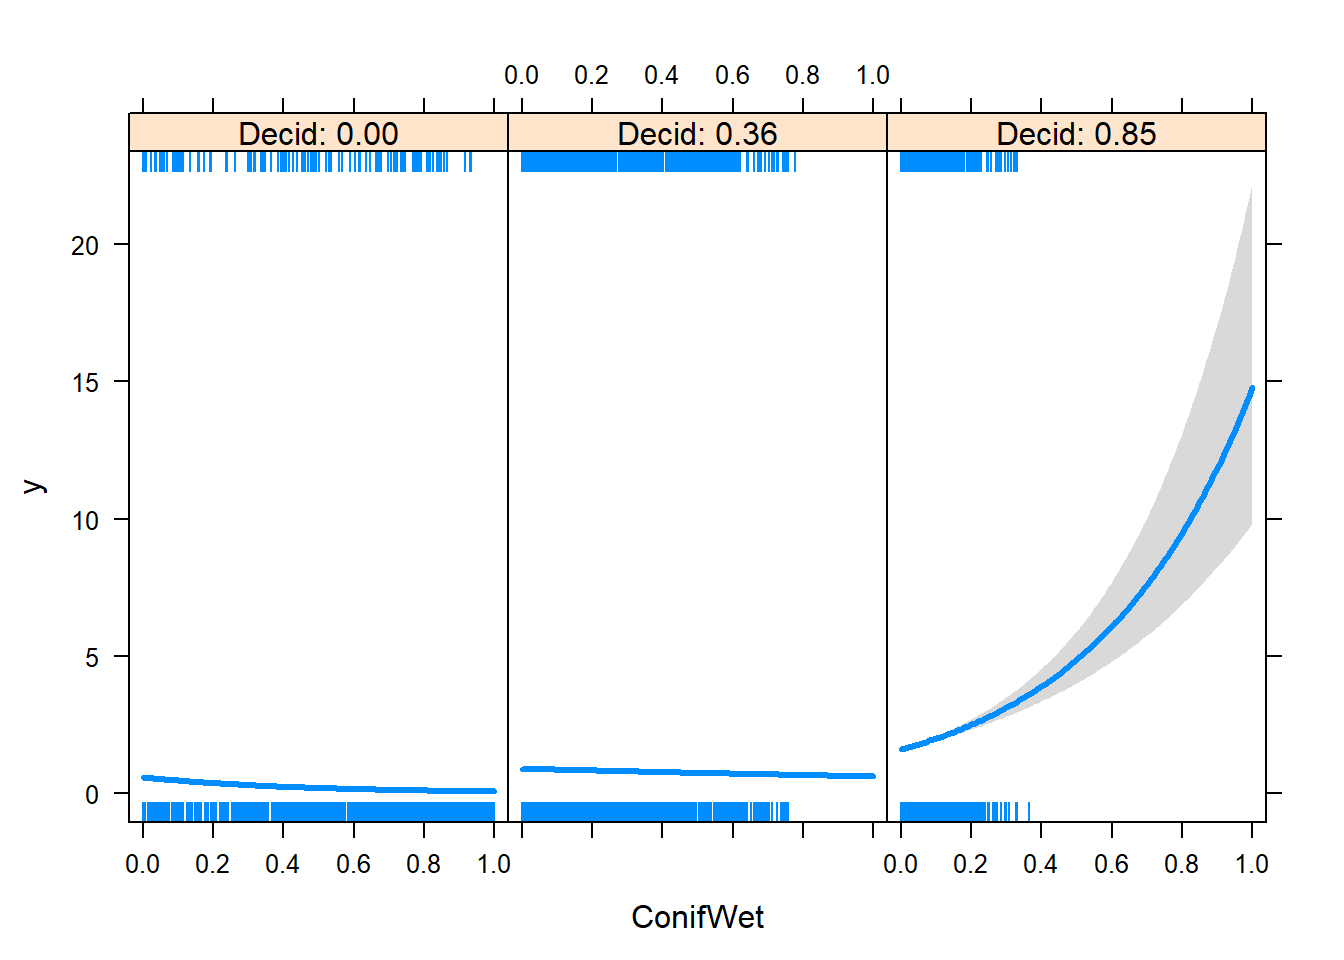
\includegraphics{qpad-book_files/figure-latex/regr-visreg2-1.pdf}

\begin{Shaded}
\begin{Highlighting}[]
\KeywordTok{mep}\NormalTok{(mP5)}
\end{Highlighting}
\end{Shaded}

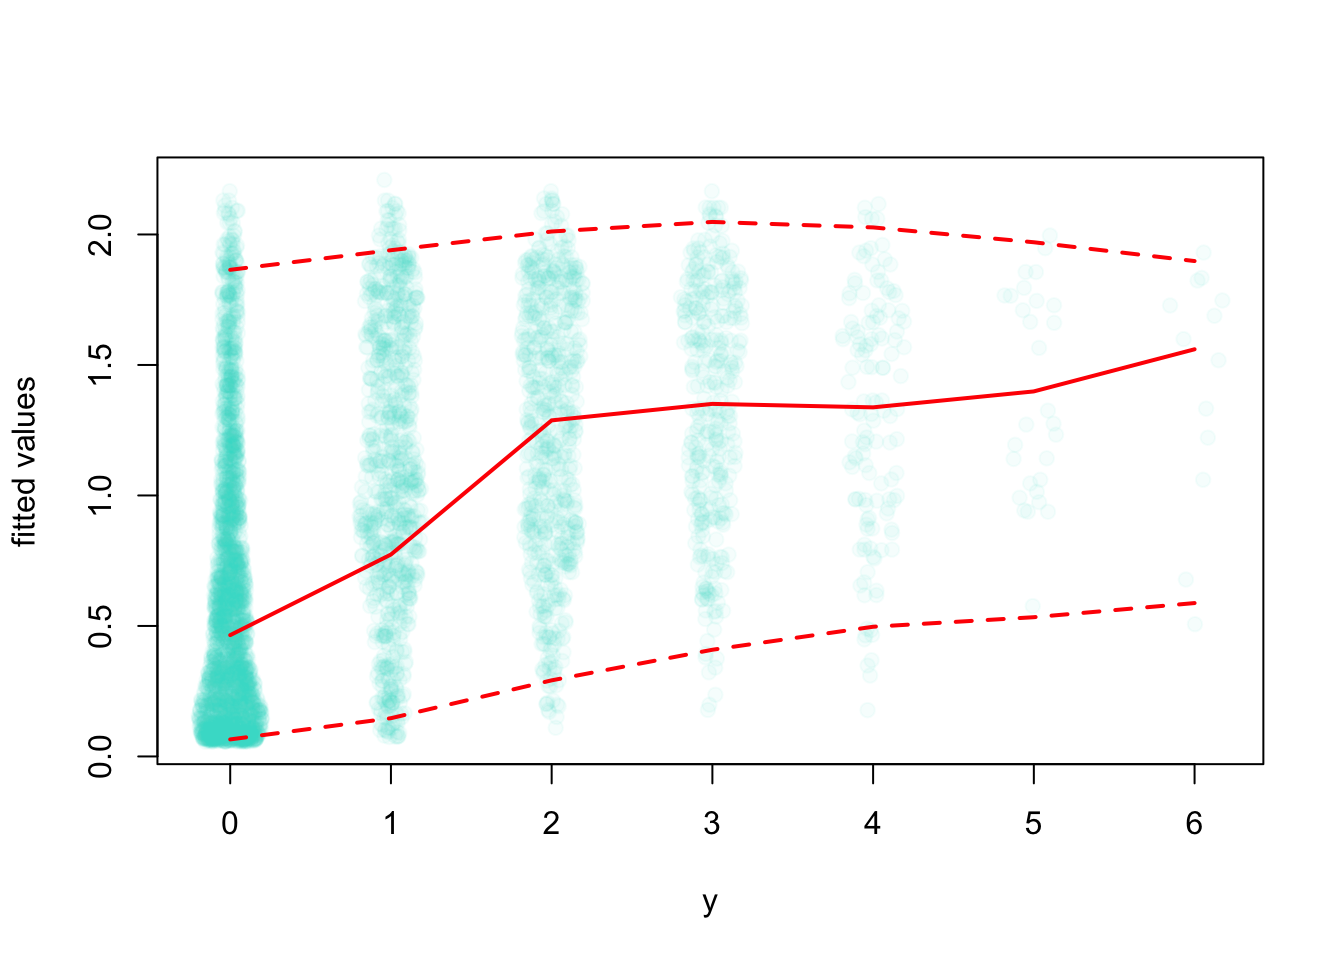
\includegraphics[width=0.33\linewidth]{qpad-book_files/figure-latex/regr-visreg3-1} 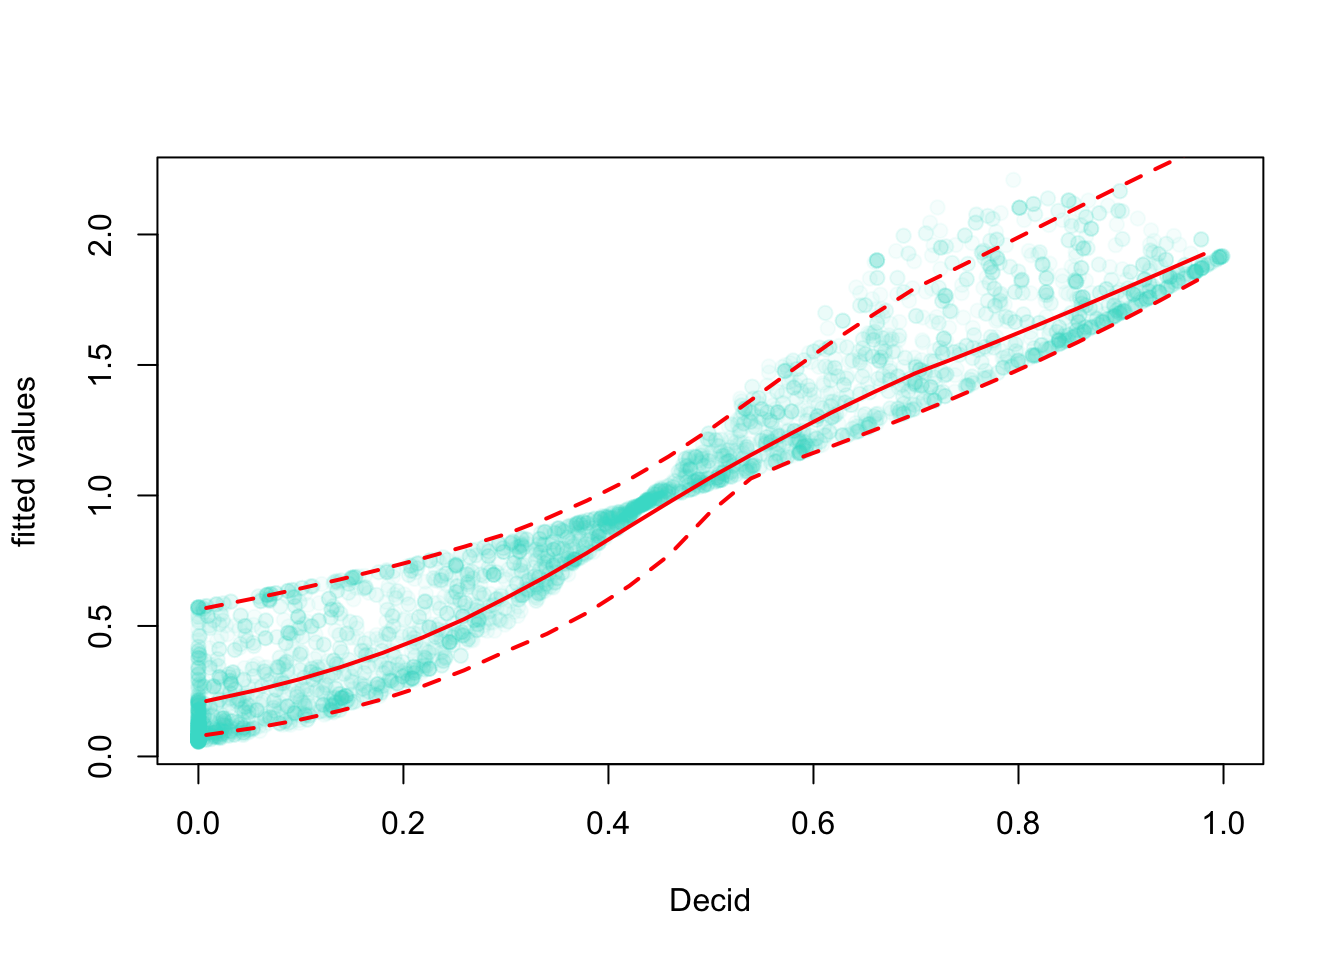
\includegraphics[width=0.33\linewidth]{qpad-book_files/figure-latex/regr-visreg3-2} 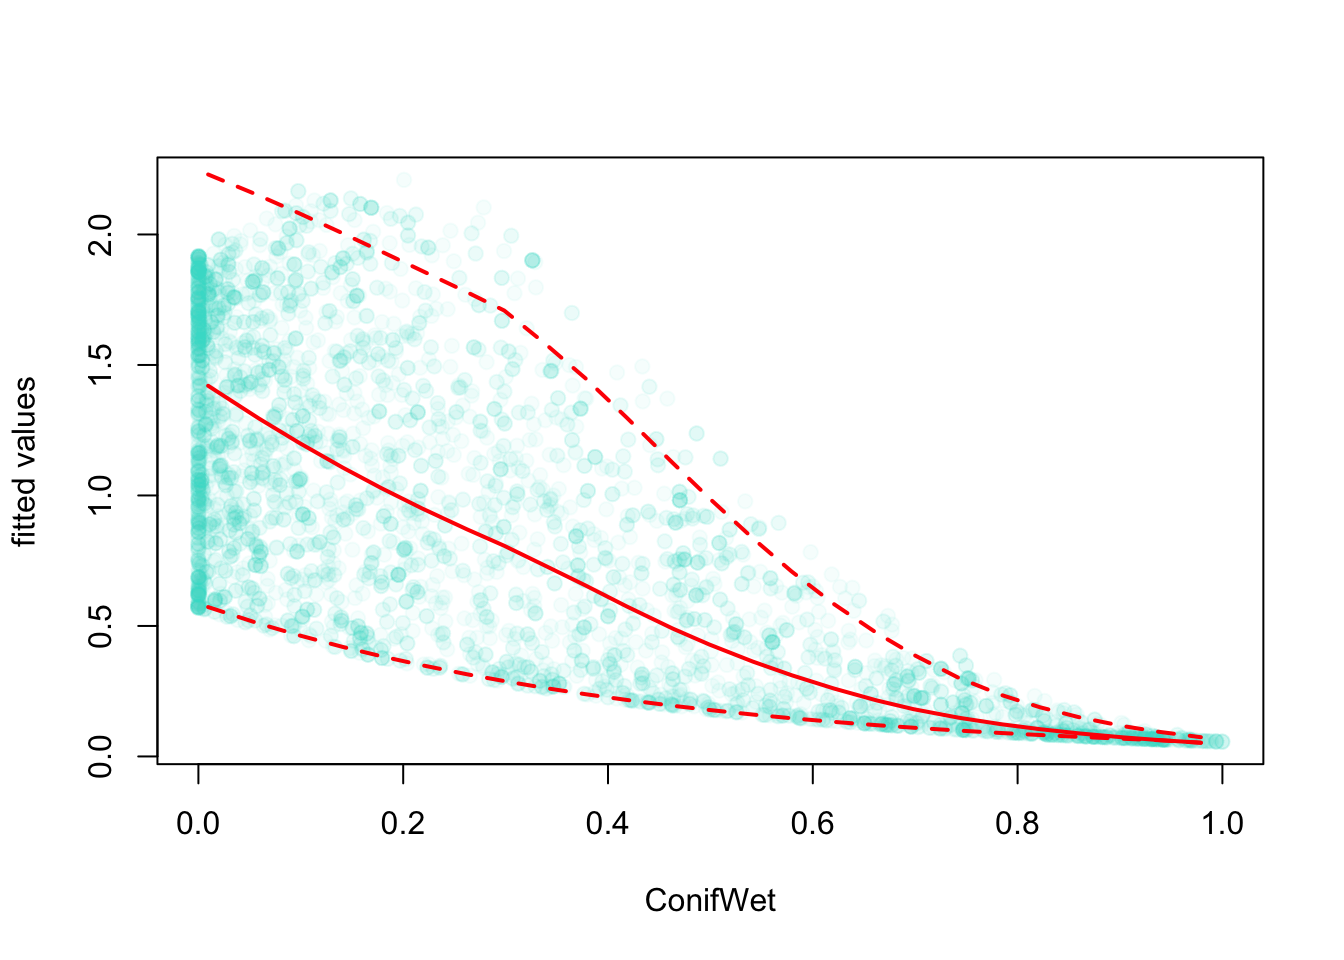
\includegraphics[width=0.33\linewidth]{qpad-book_files/figure-latex/regr-visreg3-3}

Let's use GAM to fit a bivariate spline:

\begin{Shaded}
\begin{Highlighting}[]
\NormalTok{mGAM2 <-}\StringTok{ }\NormalTok{mgcv}\OperatorTok{::}\KeywordTok{gam}\NormalTok{(y }\OperatorTok{~}\StringTok{ }\KeywordTok{s}\NormalTok{(Decid, ConifWet), }\DataTypeTok{data=}\NormalTok{x, }\DataTypeTok{family=}\NormalTok{poisson)}
\KeywordTok{plot}\NormalTok{(mGAM2, }\DataTypeTok{scheme=}\DecValTok{2}\NormalTok{, }\DataTypeTok{rug=}\OtherTok{FALSE}\NormalTok{)}
\end{Highlighting}
\end{Shaded}

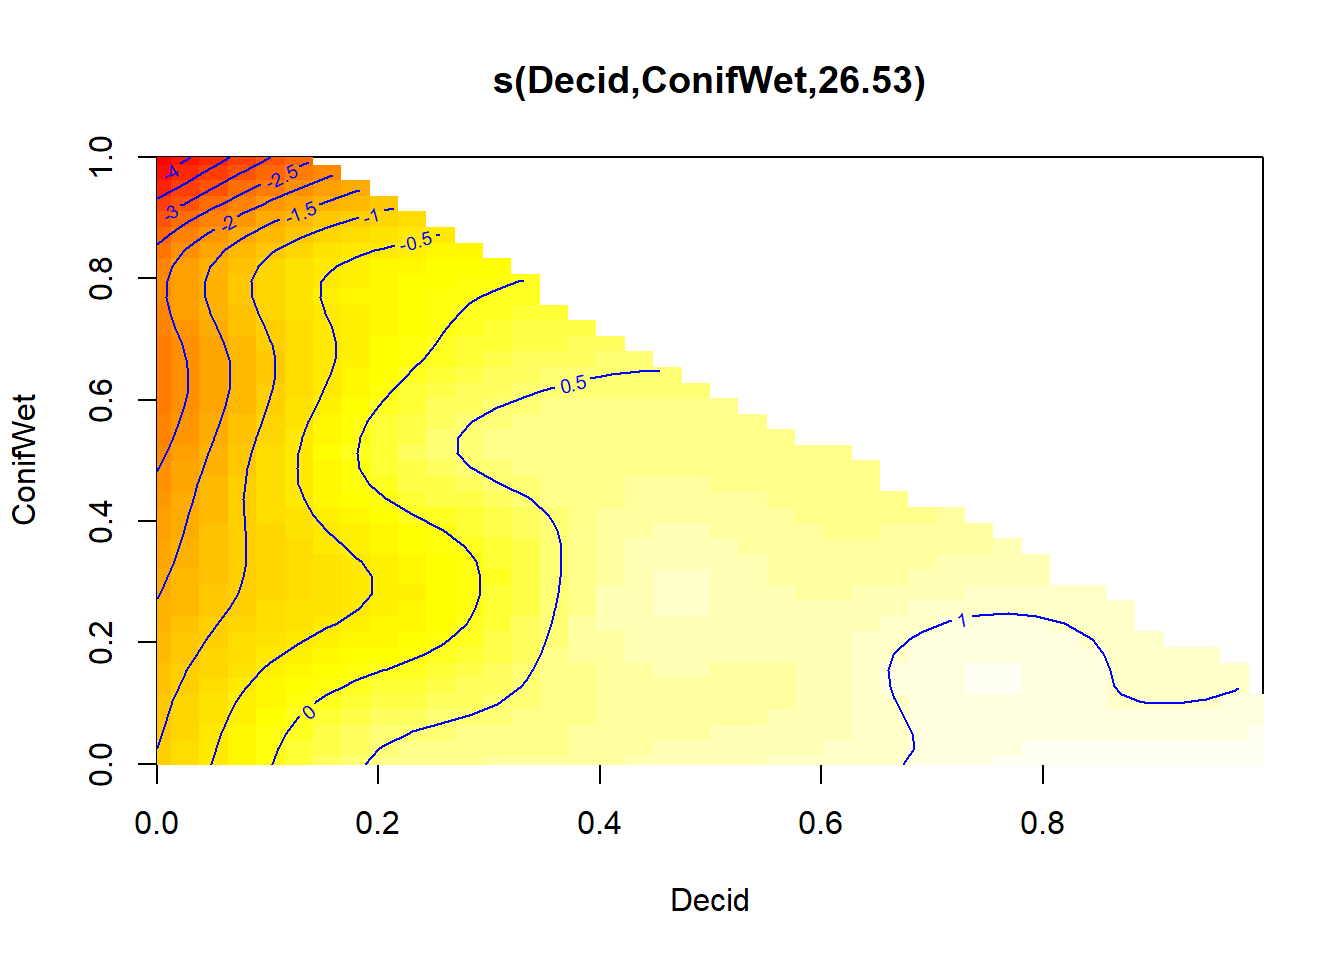
\includegraphics{qpad-book_files/figure-latex/regr-GAM2-1.pdf}

Final battle of Poisson models:

\begin{Shaded}
\begin{Highlighting}[]
\KeywordTok{model.sel}\NormalTok{(mP0, mP1, mP12, mP13, mP14, mP2, mP3, mP4, mP5, mGAM, mGAM2)}
\end{Highlighting}
\end{Shaded}

\begin{verbatim}
## Model selection table 
##         (Int)    Dcd  Dcd^2  Dcd^3  Dcd^4   DEC HAB     CnW CnW:Dcd s(Dcd)
## mGAM2 -0.6242                                                             
## mGAM  -0.5606                                                            +
## mP14  -2.6640 16.640 -38.60 41.470 -16.31                                 
## mP13  -2.3910 11.400 -16.31  8.066                                        
## mP12  -1.9240  6.259  -3.97                                               
## mP5   -0.5604  1.213                                -2.3120   5.346       
## mP4   -0.7014  1.622                                -0.9785               
## mP1   -1.1640  2.134                                                      
## mP3   -1.3860                                     +                       
## mP2   -0.8577                             1.216                           
## mP0   -0.1243                                                             
##       s(Dcd,CnW) class df logLik  AICc   delta weight
## mGAM2          +   gam 27  -5160 10376    0.00      1
## mGAM               gam  9  -5209 10438   61.73      0
## mP14               glm  5  -5215 10441   65.05      0
## mP13               glm  4  -5226 10461   85.15      0
## mP12               glm  3  -5269 10544  167.77      0
## mP5                glm  4  -5271 10549  173.62      0
## mP4                glm  3  -5392 10791  414.81      0
## mP1                glm  2  -5442 10887  511.33      0
## mP3                glm  9  -5572 11162  785.69      0
## mP2                glm  2  -5621 11246  869.98      0
## mP0                glm  1  -6285 12573 2197.20      0
## Models ranked by AICc(x)
\end{verbatim}

\begin{Shaded}
\begin{Highlighting}[]
\KeywordTok{R2dev}\NormalTok{(mP0, mP1, mP12, mP13, mP14, mP2, mP3, mP4, mP5, mGAM, mGAM2)}
\end{Highlighting}
\end{Shaded}

\begin{verbatim}
##            R2   R2adj Deviance    Dev0    DevR     df0     dfR p_value    
## mP0      0.00    0.00     0.00 7424.78 7424.78 4568.00 4568.00 < 2e-16 ***
## mP1      0.23    0.23  1687.87 7424.78 5736.91 4568.00 4567.00 < 2e-16 ***
## mP12     0.27    0.27  2033.44 7424.78 5391.34 4568.00 4566.00 < 2e-16 ***
## mP13     0.29    0.28  2118.06 7424.78 5306.72 4568.00 4565.00 7.6e-14 ***
## mP14     0.29    0.29  2140.17 7424.78 5284.61 4568.00 4564.00 3.4e-13 ***
## mP2      0.18    0.18  1329.23 7424.78 6095.55 4568.00 4567.00 < 2e-16 ***
## mP3      0.19    0.19  1427.55 7424.78 5997.23 4568.00 4560.00 < 2e-16 ***
## mP4      0.24    0.24  1786.40 7424.78 5638.38 4568.00 4566.00 < 2e-16 ***
## mP5      0.27    0.27  2029.60 7424.78 5395.18 4568.00 4565.00 < 2e-16 ***
## mGAM     0.29    0.29  2152.63 7424.78 5272.15 4568.00 4559.00 5.5e-13 ***
## mGAM2    0.30    0.30  2250.62 7424.78 5174.16 4568.00 4539.00 8.5e-11 ***
## ---
## Signif. codes:  0 '***' 0.001 '**' 0.01 '*' 0.05 '.' 0.1 ' ' 1
\end{verbatim}

Of course, the most complex model wins
but the Chi-square test is still significant (indicating lack of fit).
Let's try different error distribution.

\hypertarget{different-error-distributions}{%
\section{Different error distributions}\label{different-error-distributions}}

We will use the 2-variable model with interaction:

\begin{Shaded}
\begin{Highlighting}[]
\NormalTok{mP <-}\StringTok{ }\KeywordTok{glm}\NormalTok{(y }\OperatorTok{~}\StringTok{ }\NormalTok{Decid }\OperatorTok{*}\StringTok{ }\NormalTok{ConifWet, }\DataTypeTok{data=}\NormalTok{x, }\DataTypeTok{family=}\NormalTok{poisson)}
\end{Highlighting}
\end{Shaded}

Let us try the Negative Binomial distribution first.
This distribution is related to Binomial experiments
(number of trials required to get a fixed number of successes
given a binomial probability). It can also be derived
as a mixture of Poisson and Gamma distributions
(see \href{https://en.wikipedia.org/wiki/Negative_binomial_distribution\#Gamma\%E2\%80\%93Poisson_mixture}{Wikipedia}),
which is a kind of hierarchical model.
In this case, the Gamma distribution acts as an i.i.d.
random effect for the intercept:
\(Y_i\sim Poisson(\lambda_i)\),
\(\lambda_i \sim Gamma(e^{\beta_0+\beta_1 x_{1i}}, \gamma)\),
where \(\gamma\) is the Gamma variance.

The Negative Binomial variance (using the parametrization common in R functions)
is a function of the mean and the scale: \(V(\mu) = \mu + \mu^2/\theta\).

\begin{Shaded}
\begin{Highlighting}[]
\NormalTok{mNB <-}\StringTok{ }\KeywordTok{glm.nb}\NormalTok{(y }\OperatorTok{~}\StringTok{ }\NormalTok{Decid }\OperatorTok{*}\StringTok{ }\NormalTok{ConifWet, }\DataTypeTok{data=}\NormalTok{x)}
\KeywordTok{summary}\NormalTok{(mNB)}
\end{Highlighting}
\end{Shaded}

\begin{verbatim}
## 
## Call:
## glm.nb(formula = y ~ Decid * ConifWet, data = x, init.theta = 3.5900635, 
##     link = log)
## 
## Deviance Residuals: 
##    Min      1Q  Median      3Q     Max  
## -1.860  -0.985  -0.451   0.317   3.803  
## 
## Coefficients:
##                Estimate Std. Error z value Pr(>|z|)    
## (Intercept)     -0.5905     0.0630   -9.38   <2e-16 ***
## Decid            1.2459     0.0892   13.97   <2e-16 ***
## ConifWet        -2.3545     0.1605  -14.67   <2e-16 ***
## Decid:ConifWet   5.6945     0.4009   14.20   <2e-16 ***
## ---
## Signif. codes:  0 '***' 0.001 '**' 0.01 '*' 0.05 '.' 0.1 ' ' 1
## 
## (Dispersion parameter for Negative Binomial(3.59) family taken to be 1)
## 
##     Null deviance: 6089.3  on 4568  degrees of freedom
## Residual deviance: 4387.7  on 4565  degrees of freedom
## AIC: 10440
## 
## Number of Fisher Scoring iterations: 1
## 
## 
##               Theta:  3.590 
##           Std. Err.:  0.425 
## 
##  2 x log-likelihood:  -10430.448
\end{verbatim}

Next, we look at zero-inflated models.
In this case, the mixture distribution is a Bernoulli distribution
and a count distribution (Poisson or Negative Binomial, for example).
The 0's can come from both the zero and the count distributions,
whereas the \textgreater{}0 values can only come from the count distribution:
\(A_i \sim Bernoulli(\varphi)\), \(Y_i \sim Poisson(A_i \lambda_i)\).

The zero part of the zero-inflated models are often parametrized
as probability of zero (\(1-\varphi\)), as in the \texttt{pscl::zeroinfl} function:

\begin{Shaded}
\begin{Highlighting}[]
\CommentTok{## Zero-inflated Poisson}
\NormalTok{mZIP <-}\StringTok{ }\KeywordTok{zeroinfl}\NormalTok{(y }\OperatorTok{~}\StringTok{ }\NormalTok{Decid }\OperatorTok{*}\StringTok{ }\NormalTok{ConifWet }\OperatorTok{|}\StringTok{ }\DecValTok{1}\NormalTok{, x, }\DataTypeTok{dist=}\StringTok{"poisson"}\NormalTok{)}
\KeywordTok{summary}\NormalTok{(mZIP)}
\end{Highlighting}
\end{Shaded}

\begin{verbatim}
## 
## Call:
## zeroinfl(formula = y ~ Decid * ConifWet | 1, data = x, dist = "poisson")
## 
## Pearson residuals:
##    Min     1Q Median     3Q    Max 
## -1.218 -0.700 -0.339  0.378  8.951 
## 
## Count model coefficients (poisson with log link):
##                Estimate Std. Error z value Pr(>|z|)    
## (Intercept)     -0.3241     0.0651   -4.98  6.5e-07 ***
## Decid            1.0700     0.0860   12.44  < 2e-16 ***
## ConifWet        -2.4407     0.1564  -15.60  < 2e-16 ***
## Decid:ConifWet   5.9373     0.3840   15.46  < 2e-16 ***
## 
## Zero-inflation model coefficients (binomial with logit link):
##             Estimate Std. Error z value Pr(>|z|)    
## (Intercept)   -1.613      0.103   -15.6   <2e-16 ***
## ---
## Signif. codes:  0 '***' 0.001 '**' 0.01 '*' 0.05 '.' 0.1 ' ' 1 
## 
## Number of iterations in BFGS optimization: 12 
## Log-likelihood: -5.21e+03 on 5 Df
\end{verbatim}

\begin{Shaded}
\begin{Highlighting}[]
\CommentTok{## Zero-inflated Negative Binomial}
\NormalTok{mZINB <-}\StringTok{ }\KeywordTok{zeroinfl}\NormalTok{(y }\OperatorTok{~}\StringTok{ }\NormalTok{Decid }\OperatorTok{*}\StringTok{ }\NormalTok{ConifWet }\OperatorTok{|}\StringTok{ }\DecValTok{1}\NormalTok{, x, }\DataTypeTok{dist=}\StringTok{"negbin"}\NormalTok{)}
\KeywordTok{summary}\NormalTok{(mZINB)}
\end{Highlighting}
\end{Shaded}

\begin{verbatim}
## 
## Call:
## zeroinfl(formula = y ~ Decid * ConifWet | 1, data = x, dist = "negbin")
## 
## Pearson residuals:
##    Min     1Q Median     3Q    Max 
## -1.190 -0.689 -0.338  0.361  8.956 
## 
## Count model coefficients (negbin with log link):
##                Estimate Std. Error z value Pr(>|z|)    
## (Intercept)     -0.3873     0.0732   -5.29  1.2e-07 ***
## Decid            1.1195     0.0911   12.29  < 2e-16 ***
## ConifWet        -2.4230     0.1589  -15.25  < 2e-16 ***
## Decid:ConifWet   5.9227     0.3963   14.94  < 2e-16 ***
## Log(theta)       2.6504     0.5305    5.00  5.9e-07 ***
## 
## Zero-inflation model coefficients (binomial with logit link):
##             Estimate Std. Error z value Pr(>|z|)    
## (Intercept)   -1.861      0.193   -9.64   <2e-16 ***
## ---
## Signif. codes:  0 '***' 0.001 '**' 0.01 '*' 0.05 '.' 0.1 ' ' 1 
## 
## Theta = 14.159 
## Number of iterations in BFGS optimization: 22 
## Log-likelihood: -5.2e+03 on 6 Df
\end{verbatim}

Now we compare the four different parametric models:

\begin{Shaded}
\begin{Highlighting}[]
\KeywordTok{AIC}\NormalTok{(mP, mNB, mZIP, mZINB)}
\end{Highlighting}
\end{Shaded}

Our best model is the Zero-inflated Negative Binomial.
The probability of observing a zero as part of the zero
distribution is back transformed from the zero coefficient
using the inverse logit function:

\begin{Shaded}
\begin{Highlighting}[]
\KeywordTok{unname}\NormalTok{(}\KeywordTok{plogis}\NormalTok{(}\KeywordTok{coef}\NormalTok{(mZINB, }\StringTok{"zero"}\NormalTok{))) }\CommentTok{# P of 0}
\end{Highlighting}
\end{Shaded}

\begin{verbatim}
## [1] 0.1346
\end{verbatim}

Now we use the scale parameter to visualize the variance functions
for the Negative Binomial models (the 1:1 line is the Poisson model):

\begin{Shaded}
\begin{Highlighting}[]
\NormalTok{mNB}\OperatorTok{$}\NormalTok{theta}
\end{Highlighting}
\end{Shaded}

\begin{verbatim}
## [1] 3.59
\end{verbatim}

\begin{Shaded}
\begin{Highlighting}[]
\NormalTok{mZINB}\OperatorTok{$}\NormalTok{theta}
\end{Highlighting}
\end{Shaded}

\begin{verbatim}
## [1] 14.16
\end{verbatim}

\begin{Shaded}
\begin{Highlighting}[]
\NormalTok{mu <-}\StringTok{ }\KeywordTok{seq}\NormalTok{(}\DecValTok{0}\NormalTok{, }\DecValTok{5}\NormalTok{, }\FloatTok{0.01}\NormalTok{)}
\KeywordTok{plot}\NormalTok{(mu, mu }\OperatorTok{+}\StringTok{ }\NormalTok{mu}\OperatorTok{^}\DecValTok{2}\OperatorTok{/}\NormalTok{mNB}\OperatorTok{$}\NormalTok{theta, }\DataTypeTok{type=}\StringTok{"l"}\NormalTok{, }\DataTypeTok{col=}\DecValTok{2}\NormalTok{,}
  \DataTypeTok{ylab=}\KeywordTok{expression}\NormalTok{(}\KeywordTok{V}\NormalTok{(mu)), }\DataTypeTok{xlab=}\KeywordTok{expression}\NormalTok{(mu))}
\KeywordTok{lines}\NormalTok{(mu, mu }\OperatorTok{+}\StringTok{ }\NormalTok{mu}\OperatorTok{^}\DecValTok{2}\OperatorTok{/}\NormalTok{mZINB}\OperatorTok{$}\NormalTok{theta, }\DataTypeTok{type=}\StringTok{"l"}\NormalTok{, }\DataTypeTok{col=}\DecValTok{4}\NormalTok{)}
\KeywordTok{abline}\NormalTok{(}\DecValTok{0}\NormalTok{,}\DecValTok{1}\NormalTok{, }\DataTypeTok{lty=}\DecValTok{2}\NormalTok{)}
\KeywordTok{legend}\NormalTok{(}\StringTok{"topleft"}\NormalTok{, }\DataTypeTok{bty=}\StringTok{"n"}\NormalTok{, }\DataTypeTok{lty=}\DecValTok{1}\NormalTok{, }\DataTypeTok{col=}\KeywordTok{c}\NormalTok{(}\DecValTok{2}\NormalTok{,}\DecValTok{4}\NormalTok{),}
  \DataTypeTok{legend=}\KeywordTok{paste}\NormalTok{(}\KeywordTok{c}\NormalTok{(}\StringTok{"NB"}\NormalTok{, }\StringTok{"ZINB"}\NormalTok{), }\KeywordTok{round}\NormalTok{(}\KeywordTok{c}\NormalTok{(mNB}\OperatorTok{$}\NormalTok{theta, mZINB}\OperatorTok{$}\NormalTok{theta), }\DecValTok{2}\NormalTok{)))}
\end{Highlighting}
\end{Shaded}

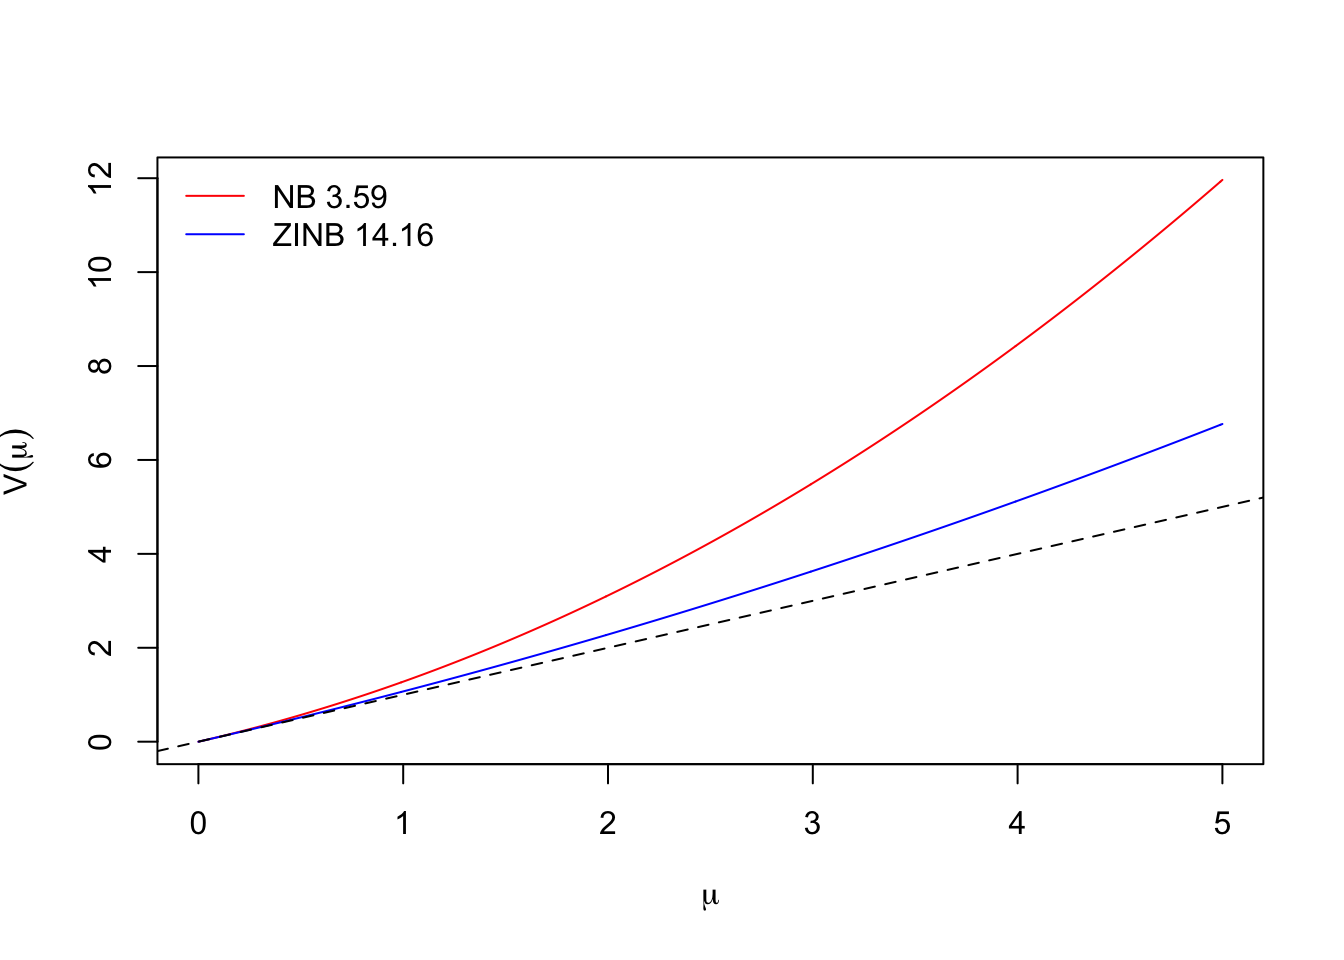
\includegraphics{qpad-book_files/figure-latex/regr-dist6-1.pdf}

\BeginKnitrBlock{rmdexercise}
\textbf{Exercise}

How can we interpret these different kinds of overdispersion (zero-inflation and higher than Poisson variance)?

What are some of the biological mechanisms that can contribute to the
overdispersion?
\EndKnitrBlock{rmdexercise}

It is also common practice to consider generalized linear mixed models (GLMMs)
for count data. These mixed models are usually considered as
Poisson-Lognormal mixtures. The simplest, so called i.i.d., case
is similar to the Negative Binomial, but instead of Gamma, we have Lognormal
distribution:
\(Y_i\sim Poisson(\lambda_i)\),
\(log(\lambda_i) = \beta_0+\beta_1 x_{1i}+\epsilon_i\),
\(\epsilon_i \sim Normal(0, \sigma^2)\),
where \(\sigma^2\) is the Lognormal variance on the log scale.

We can use the \texttt{lme4::glmer} function: use \texttt{SiteID} as random effect
(we have exactly \(n\) random effects).

\begin{Shaded}
\begin{Highlighting}[]
\NormalTok{mPLN1 <-}\StringTok{ }\KeywordTok{glmer}\NormalTok{(y }\OperatorTok{~}\StringTok{ }\NormalTok{Decid }\OperatorTok{*}\StringTok{ }\NormalTok{ConifWet }\OperatorTok{+}\StringTok{ }\NormalTok{(}\DecValTok{1} \OperatorTok{|}\StringTok{ }\NormalTok{SiteID), }\DataTypeTok{data=}\NormalTok{x, }\DataTypeTok{family=}\NormalTok{poisson)}
\KeywordTok{summary}\NormalTok{(mPLN1)}
\end{Highlighting}
\end{Shaded}

\begin{verbatim}
## Generalized linear mixed model fit by maximum likelihood (Laplace
##   Approximation) [glmerMod]
##  Family: poisson  ( log )
## Formula: y ~ Decid * ConifWet + (1 | SiteID)
##    Data: x
## 
##      AIC      BIC   logLik deviance df.resid 
##    10423    10455    -5206    10413     4564 
## 
## Scaled residuals: 
##    Min     1Q Median     3Q    Max 
## -1.150 -0.629 -0.288  0.418  5.469 
## 
## Random effects:
##  Groups Name        Variance Std.Dev.
##  SiteID (Intercept) 0.294    0.542   
## Number of obs: 4569, groups:  SiteID, 4569
## 
## Fixed effects:
##                Estimate Std. Error z value Pr(>|z|)    
## (Intercept)     -0.7518     0.0675   -11.1   <2e-16 ***
## Decid            1.2847     0.0920    14.0   <2e-16 ***
## ConifWet        -2.3380     0.1625   -14.4   <2e-16 ***
## Decid:ConifWet   5.6326     0.4119    13.7   <2e-16 ***
## ---
## Signif. codes:  0 '***' 0.001 '**' 0.01 '*' 0.05 '.' 0.1 ' ' 1
## 
## Correlation of Fixed Effects:
##             (Intr) Decid  ConfWt
## Decid       -0.895              
## ConifWet    -0.622  0.644       
## Decid:CnfWt  0.176 -0.379 -0.700
\end{verbatim}

\BeginKnitrBlock{rmdnote}
\textbf{Note}

The number of unknowns we have to somehow estimate is now more than the number of observations we have. How is that possible?
\EndKnitrBlock{rmdnote}

Alternatively, we can use \texttt{SurveyArea} as a grouping variable.
We have now \(m < n\) random effects, and survey areas can be seen
as larger landscapes within which the sites are clustered:
\(Y_ij\sim Poisson(\lambda_ij)\),
\(log(\lambda_ij) = \beta_0+\beta_1 x_{1ij}+\epsilon_i\),
\(\epsilon_i \sim Normal(0, \sigma^2)\).
The index \(i\) (\(i=1,...,m\)) defines the cluster (survey area),
the \(j\) (\(j=1,...,n_i\)) defines the sites within survey area \(i\)
(\(n = \sum_{i=1}^m n_i\)).

\begin{Shaded}
\begin{Highlighting}[]
\NormalTok{mPLN2 <-}\StringTok{ }\KeywordTok{glmer}\NormalTok{(y }\OperatorTok{~}\StringTok{ }\NormalTok{Decid }\OperatorTok{*}\StringTok{ }\NormalTok{ConifWet }\OperatorTok{+}\StringTok{ }\NormalTok{(}\DecValTok{1} \OperatorTok{|}\StringTok{ }\NormalTok{SurveyArea), }\DataTypeTok{data=}\NormalTok{x, }\DataTypeTok{family=}\NormalTok{poisson)}
\KeywordTok{summary}\NormalTok{(mPLN2)}
\end{Highlighting}
\end{Shaded}

\begin{verbatim}
## Generalized linear mixed model fit by maximum likelihood (Laplace
##   Approximation) [glmerMod]
##  Family: poisson  ( log )
## Formula: y ~ Decid * ConifWet + (1 | SurveyArea)
##    Data: x
## 
##      AIC      BIC   logLik deviance df.resid 
##    10021    10053    -5006    10011     4564 
## 
## Scaled residuals: 
##    Min     1Q Median     3Q    Max 
## -1.739 -0.643 -0.320  0.355  6.535 
## 
## Random effects:
##  Groups     Name        Variance Std.Dev.
##  SurveyArea (Intercept) 0.295    0.543   
## Number of obs: 4569, groups:  SurveyArea, 271
## 
## Fixed effects:
##                Estimate Std. Error z value Pr(>|z|)    
## (Intercept)     -0.7459     0.0783   -9.53   <2e-16 ***
## Decid            1.1967     0.0984   12.16   <2e-16 ***
## ConifWet        -2.3213     0.1687  -13.76   <2e-16 ***
## Decid:ConifWet   5.5346     0.3978   13.91   <2e-16 ***
## ---
## Signif. codes:  0 '***' 0.001 '**' 0.01 '*' 0.05 '.' 0.1 ' ' 1
## 
## Correlation of Fixed Effects:
##             (Intr) Decid  ConfWt
## Decid       -0.808              
## ConifWet    -0.610  0.628       
## Decid:CnfWt  0.162 -0.325 -0.670
\end{verbatim}

In the battle of distributions (keeping the linear predictor
part the same) the clustered GLMM was best supported:

\begin{Shaded}
\begin{Highlighting}[]
\NormalTok{tmp <-}\StringTok{ }\KeywordTok{AIC}\NormalTok{(mP, mNB, mZIP, mZINB, mPLN1, mPLN2)}
\NormalTok{tmp}\OperatorTok{$}\NormalTok{delta_AIC <-}\StringTok{ }\NormalTok{tmp}\OperatorTok{$}\NormalTok{AIC }\OperatorTok{-}\StringTok{ }\KeywordTok{min}\NormalTok{(tmp}\OperatorTok{$}\NormalTok{AIC)}
\NormalTok{tmp[}\KeywordTok{order}\NormalTok{(tmp}\OperatorTok{$}\NormalTok{AIC),]}
\end{Highlighting}
\end{Shaded}

\BeginKnitrBlock{rmdexercise}
\textbf{Exercise}

What are some of the biological mechanisms that can lead to the
clustered GLMM bi be the best model?
\EndKnitrBlock{rmdexercise}

\hypertarget{count-duration-effects}{%
\section{Count duration effects}\label{count-duration-effects}}

Let's change gears a bit now, and steer closer to the main focus
of this book. We want to account for methodological differences
among samples. One aspect of mathodologies involve
variation in total counting duration. We'll now inspect what
that does to our observations.

First, we create a list of matrices where counts are
tabulated by surveys and time intervals for each species:

\begin{Shaded}
\begin{Highlighting}[]
\NormalTok{ydur <-}\StringTok{ }\KeywordTok{Xtab}\NormalTok{(}\OperatorTok{~}\StringTok{ }\NormalTok{SiteID }\OperatorTok{+}\StringTok{ }\NormalTok{Dur }\OperatorTok{+}\StringTok{ }\NormalTok{SpeciesID , }
\NormalTok{  josm}\OperatorTok{$}\NormalTok{counts[josm}\OperatorTok{$}\NormalTok{counts}\OperatorTok{$}\NormalTok{DetectType1 }\OperatorTok{!=}\StringTok{ "V"}\NormalTok{,])}
\end{Highlighting}
\end{Shaded}

We use the same species (\texttt{spp}) as before and create a
data frame indluring the cumulative counts during 3, 5, and 10 minutes:

\begin{Shaded}
\begin{Highlighting}[]
\NormalTok{y <-}\StringTok{ }\KeywordTok{as.matrix}\NormalTok{(ydur[[spp]])}
\KeywordTok{head}\NormalTok{(y)}
\end{Highlighting}
\end{Shaded}

\begin{verbatim}
##         0-3min 3-5min 5-10min
## CL10102      3      0       0
## CL10106      0      0       0
## CL10108      0      0       0
## CL10109      2      0       1
## CL10111      2      0       0
## CL10112      2      0       0
\end{verbatim}

\begin{Shaded}
\begin{Highlighting}[]
\KeywordTok{colMeans}\NormalTok{(y) }\CommentTok{# mean count of new individuals}
\end{Highlighting}
\end{Shaded}

\begin{verbatim}
##  0-3min  3-5min 5-10min 
## 0.67367 0.09346 0.11600
\end{verbatim}

\begin{Shaded}
\begin{Highlighting}[]
\KeywordTok{cumsum}\NormalTok{(}\KeywordTok{colMeans}\NormalTok{(y)) }\CommentTok{# cumulative counts}
\end{Highlighting}
\end{Shaded}

\begin{verbatim}
##  0-3min  3-5min 5-10min 
##  0.6737  0.7671  0.8831
\end{verbatim}

\begin{Shaded}
\begin{Highlighting}[]
\NormalTok{x <-}\StringTok{ }\KeywordTok{data.frame}\NormalTok{(}
\NormalTok{  josm}\OperatorTok{$}\NormalTok{surveys, }
  \DataTypeTok{y3=}\NormalTok{y[,}\StringTok{"0-3min"}\NormalTok{],}
  \DataTypeTok{y5=}\NormalTok{y[,}\StringTok{"0-3min"}\NormalTok{]}\OperatorTok{+}\NormalTok{y[,}\StringTok{"3-5min"}\NormalTok{],}
  \DataTypeTok{y10=}\KeywordTok{rowSums}\NormalTok{(y))}

\KeywordTok{table}\NormalTok{(x}\OperatorTok{$}\NormalTok{y3)}
\end{Highlighting}
\end{Shaded}

\begin{verbatim}
## 
##    0    1    2    3    4    5    6 
## 2768  922  576  226   61   14    2
\end{verbatim}

\begin{Shaded}
\begin{Highlighting}[]
\KeywordTok{table}\NormalTok{(x}\OperatorTok{$}\NormalTok{y5)}
\end{Highlighting}
\end{Shaded}

\begin{verbatim}
## 
##    0    1    2    3    4    5    6 
## 2643  894  632  285   87   24    4
\end{verbatim}

\begin{Shaded}
\begin{Highlighting}[]
\KeywordTok{table}\NormalTok{(x}\OperatorTok{$}\NormalTok{y10)}
\end{Highlighting}
\end{Shaded}

\begin{verbatim}
## 
##    0    1    2    3    4    5    6 
## 2493  883  656  363  132   29   13
\end{verbatim}

If we fit single-predictor GLMs to these 3 responses, we get
different fitted values, consistent with our mean counts:

\begin{Shaded}
\begin{Highlighting}[]
\NormalTok{m3 <-}\StringTok{ }\KeywordTok{glm}\NormalTok{(y3 }\OperatorTok{~}\StringTok{ }\NormalTok{Decid, }\DataTypeTok{data=}\NormalTok{x, }\DataTypeTok{family=}\NormalTok{poisson)}
\NormalTok{m5 <-}\StringTok{ }\KeywordTok{glm}\NormalTok{(y5 }\OperatorTok{~}\StringTok{ }\NormalTok{Decid, }\DataTypeTok{data=}\NormalTok{x, }\DataTypeTok{family=}\NormalTok{poisson)}
\NormalTok{m10 <-}\StringTok{ }\KeywordTok{glm}\NormalTok{(y10 }\OperatorTok{~}\StringTok{ }\NormalTok{Decid, }\DataTypeTok{data=}\NormalTok{x, }\DataTypeTok{family=}\NormalTok{poisson)}
\KeywordTok{mean}\NormalTok{(}\KeywordTok{fitted}\NormalTok{(m3))}
\end{Highlighting}
\end{Shaded}

\begin{verbatim}
## [1] 0.6737
\end{verbatim}

\begin{Shaded}
\begin{Highlighting}[]
\KeywordTok{mean}\NormalTok{(}\KeywordTok{fitted}\NormalTok{(m5))}
\end{Highlighting}
\end{Shaded}

\begin{verbatim}
## [1] 0.7671
\end{verbatim}

\begin{Shaded}
\begin{Highlighting}[]
\KeywordTok{mean}\NormalTok{(}\KeywordTok{fitted}\NormalTok{(m10))}
\end{Highlighting}
\end{Shaded}

\begin{verbatim}
## [1] 0.8831
\end{verbatim}

Using the multiple time interval data, we can pretend that
we have a mix of methodologies with respect to count duration:

\begin{Shaded}
\begin{Highlighting}[]
\KeywordTok{set.seed}\NormalTok{(}\DecValTok{1}\NormalTok{)}
\NormalTok{x}\OperatorTok{$}\NormalTok{meth <-}\StringTok{ }\KeywordTok{as.factor}\NormalTok{(}\KeywordTok{sample}\NormalTok{(}\KeywordTok{c}\NormalTok{(}\StringTok{"A"}\NormalTok{, }\StringTok{"B"}\NormalTok{, }\StringTok{"C"}\NormalTok{), }\KeywordTok{nrow}\NormalTok{(x), }\DataTypeTok{replace=}\OtherTok{TRUE}\NormalTok{))}
\NormalTok{x}\OperatorTok{$}\NormalTok{y <-}\StringTok{ }\NormalTok{x}\OperatorTok{$}\NormalTok{y3}
\NormalTok{x}\OperatorTok{$}\NormalTok{y[x}\OperatorTok{$}\NormalTok{meth }\OperatorTok{==}\StringTok{ "B"}\NormalTok{] <-}\StringTok{ }\NormalTok{x}\OperatorTok{$}\NormalTok{y5[x}\OperatorTok{$}\NormalTok{meth }\OperatorTok{==}\StringTok{ "B"}\NormalTok{]}
\NormalTok{x}\OperatorTok{$}\NormalTok{y[x}\OperatorTok{$}\NormalTok{meth }\OperatorTok{==}\StringTok{ "C"}\NormalTok{] <-}\StringTok{ }\NormalTok{x}\OperatorTok{$}\NormalTok{y10[x}\OperatorTok{$}\NormalTok{meth }\OperatorTok{==}\StringTok{ "C"}\NormalTok{]}
\KeywordTok{boxplot}\NormalTok{(y }\OperatorTok{~}\StringTok{ }\NormalTok{meth, x)}
\NormalTok{sb <-}\StringTok{ }\KeywordTok{sum_by}\NormalTok{(x}\OperatorTok{$}\NormalTok{y, x}\OperatorTok{$}\NormalTok{meth)}
\KeywordTok{points}\NormalTok{(}\DecValTok{1}\OperatorTok{:}\DecValTok{3}\NormalTok{, sb[,}\DecValTok{1}\NormalTok{]}\OperatorTok{/}\NormalTok{sb[,}\DecValTok{2}\NormalTok{], }\DataTypeTok{col=}\DecValTok{2}\NormalTok{, }\DataTypeTok{type=}\StringTok{"b"}\NormalTok{, }\DataTypeTok{pch=}\DecValTok{4}\NormalTok{)}
\end{Highlighting}
\end{Shaded}

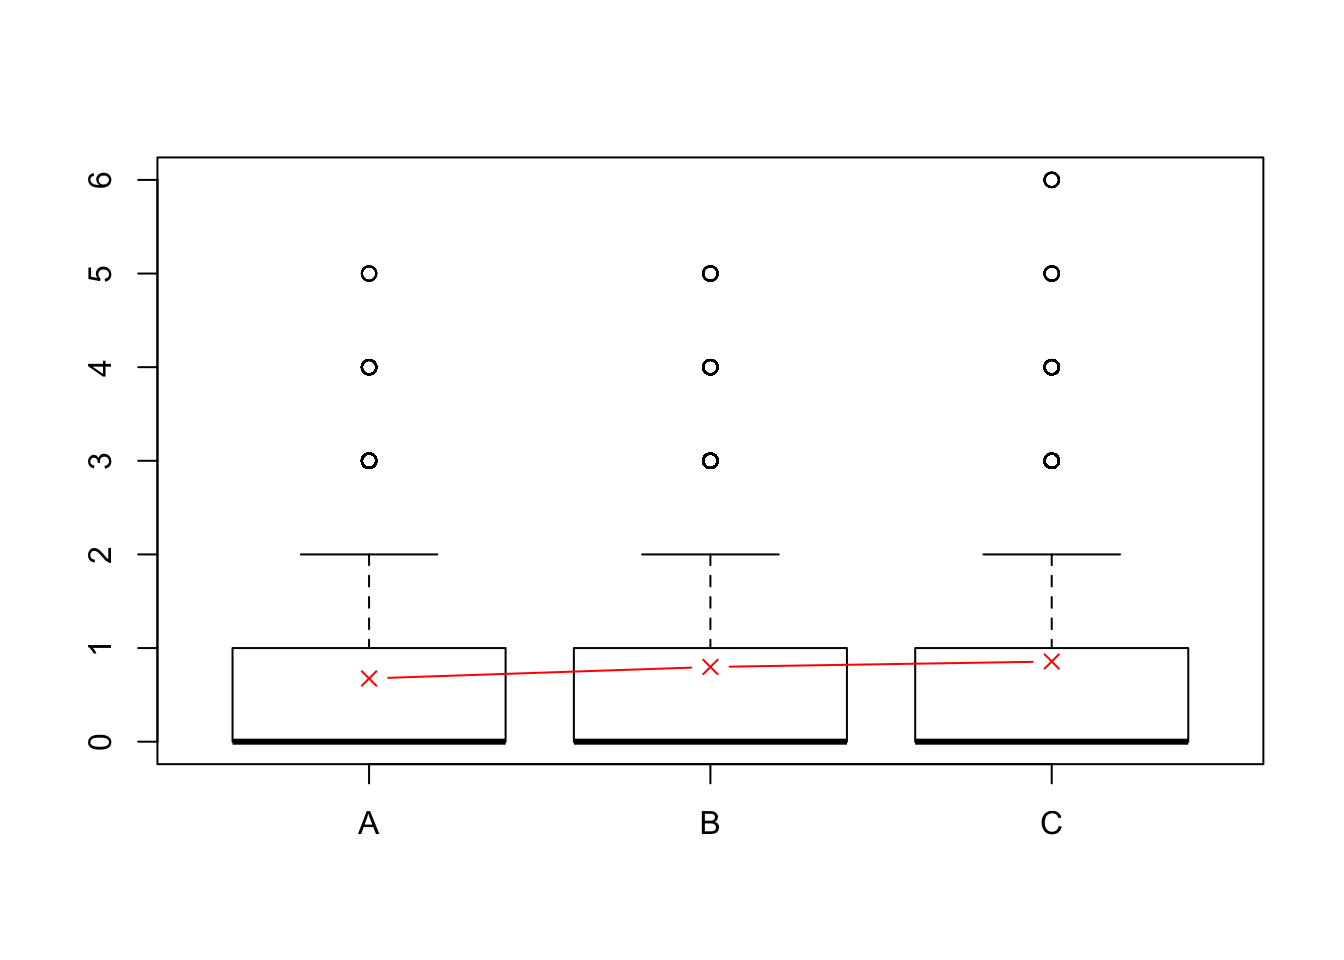
\includegraphics{qpad-book_files/figure-latex/regr-time4-1.pdf}

We can estimate the effect of the methodology:

\begin{Shaded}
\begin{Highlighting}[]
\NormalTok{mm <-}\StringTok{ }\KeywordTok{glm}\NormalTok{(y }\OperatorTok{~}\StringTok{ }\NormalTok{meth }\OperatorTok{-}\StringTok{ }\DecValTok{1}\NormalTok{, }\DataTypeTok{data=}\NormalTok{x, }\DataTypeTok{family=}\NormalTok{poisson)}
\KeywordTok{summary}\NormalTok{(mm)}
\end{Highlighting}
\end{Shaded}

\begin{verbatim}
## 
## Call:
## glm(formula = y ~ meth - 1, family = poisson, data = x)
## 
## Deviance Residuals: 
##    Min      1Q  Median      3Q     Max  
## -1.312  -1.273  -1.147   0.391   3.980  
## 
## Coefficients:
##       Estimate Std. Error z value Pr(>|z|)    
## methA  -0.4186     0.0314  -13.32  < 2e-16 ***
## methB  -0.2100     0.0282   -7.44  1.0e-13 ***
## methC  -0.1502     0.0280   -5.37  7.9e-08 ***
## ---
## Signif. codes:  0 '***' 0.001 '**' 0.01 '*' 0.05 '.' 0.1 ' ' 1
## 
## (Dispersion parameter for poisson family taken to be 1)
## 
##     Null deviance: 7233.2  on 4569  degrees of freedom
## Residual deviance: 6938.6  on 4566  degrees of freedom
## AIC: 11646
## 
## Number of Fisher Scoring iterations: 6
\end{verbatim}

\begin{Shaded}
\begin{Highlighting}[]
\KeywordTok{exp}\NormalTok{(}\KeywordTok{coef}\NormalTok{(mm))}
\end{Highlighting}
\end{Shaded}

\begin{verbatim}
##  methA  methB  methC 
## 0.6580 0.8106 0.8605
\end{verbatim}

Or the effect of the continuous predictor and the method (discrete):

\begin{Shaded}
\begin{Highlighting}[]
\NormalTok{mm <-}\StringTok{ }\KeywordTok{glm}\NormalTok{(y }\OperatorTok{~}\StringTok{ }\NormalTok{Decid }\OperatorTok{+}\StringTok{ }\NormalTok{meth, }\DataTypeTok{data=}\NormalTok{x, }\DataTypeTok{family=}\NormalTok{poisson)}
\KeywordTok{summary}\NormalTok{(mm)}
\end{Highlighting}
\end{Shaded}

\begin{verbatim}
## 
## Call:
## glm(formula = y ~ Decid + meth, family = poisson, data = x)
## 
## Deviance Residuals: 
##    Min      1Q  Median      3Q     Max  
## -2.279  -0.953  -0.740   0.447   4.568  
## 
## Coefficients:
##             Estimate Std. Error z value Pr(>|z|)    
## (Intercept)  -1.4616     0.0460  -31.80  < 2e-16 ***
## Decid         2.1450     0.0573   37.41  < 2e-16 ***
## methB         0.1669     0.0423    3.95  7.9e-05 ***
## methC         0.3027     0.0421    7.19  6.4e-13 ***
## ---
## Signif. codes:  0 '***' 0.001 '**' 0.01 '*' 0.05 '.' 0.1 ' ' 1
## 
## (Dispersion parameter for poisson family taken to be 1)
## 
##     Null deviance: 6983.3  on 4568  degrees of freedom
## Residual deviance: 5443.8  on 4565  degrees of freedom
## AIC: 10153
## 
## Number of Fisher Scoring iterations: 6
\end{verbatim}

\begin{Shaded}
\begin{Highlighting}[]
\KeywordTok{boxplot}\NormalTok{(}\KeywordTok{fitted}\NormalTok{(mm) }\OperatorTok{~}\StringTok{ }\NormalTok{meth, x)}
\end{Highlighting}
\end{Shaded}

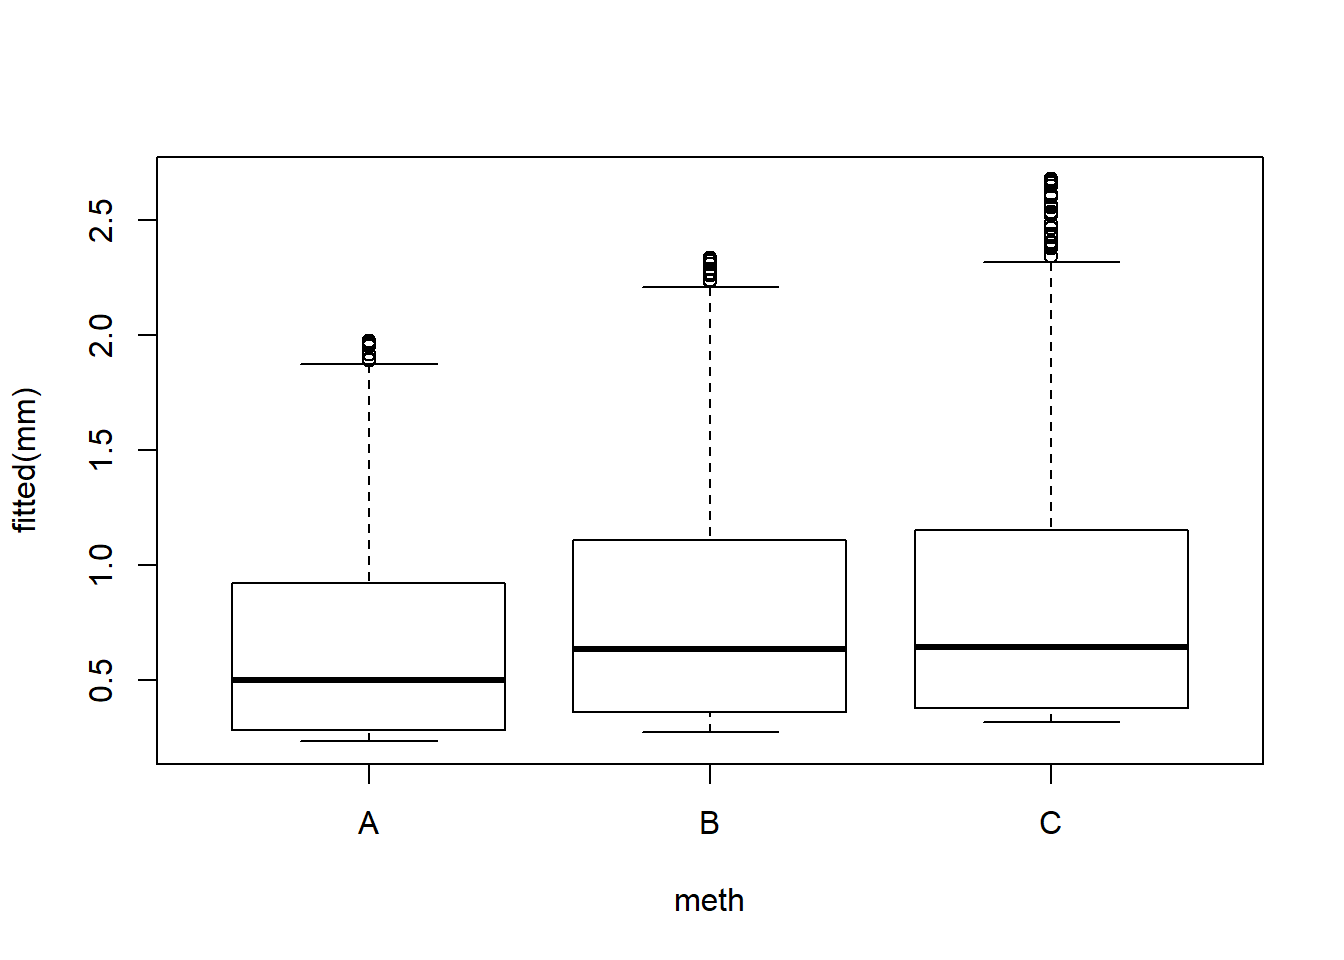
\includegraphics{qpad-book_files/figure-latex/regr-time6-1.pdf}

\begin{Shaded}
\begin{Highlighting}[]
\KeywordTok{exp}\NormalTok{(}\KeywordTok{coef}\NormalTok{(mm))}
\end{Highlighting}
\end{Shaded}

\begin{verbatim}
## (Intercept)       Decid       methB       methC 
##      0.2319      8.5421      1.1816      1.3535
\end{verbatim}

The fixed effects adjusts the means well:

\begin{Shaded}
\begin{Highlighting}[]
\KeywordTok{cumsum}\NormalTok{(}\KeywordTok{colMeans}\NormalTok{(y))}
\end{Highlighting}
\end{Shaded}

\begin{verbatim}
##  0-3min  3-5min 5-10min 
##  0.6737  0.7671  0.8831
\end{verbatim}

\begin{Shaded}
\begin{Highlighting}[]
\KeywordTok{mean}\NormalTok{(y[,}\DecValTok{1}\NormalTok{]) }\OperatorTok{*}\StringTok{ }\KeywordTok{c}\NormalTok{(}\DecValTok{1}\NormalTok{, }\KeywordTok{exp}\NormalTok{(}\KeywordTok{coef}\NormalTok{(mm))[}\DecValTok{3}\OperatorTok{:}\DecValTok{4}\NormalTok{])}
\end{Highlighting}
\end{Shaded}

\begin{verbatim}
##         methB  methC 
## 0.6737 0.7960 0.9118
\end{verbatim}

But it is all relative, depends on reference methodology/protocol.
The problem is, we can't easily extrapolate to a methodology
with count duration of 12 minutes, or interpolate to a mathodology
with count duration of 2 or 8 minutes.
We need somehow to express time expediture in minutes to make that work.
Let's try something else:

\begin{Shaded}
\begin{Highlighting}[]
\NormalTok{x}\OperatorTok{$}\NormalTok{tmax <-}\StringTok{ }\KeywordTok{c}\NormalTok{(}\DecValTok{3}\NormalTok{, }\DecValTok{5}\NormalTok{, }\DecValTok{10}\NormalTok{)[}\KeywordTok{as.integer}\NormalTok{(x}\OperatorTok{$}\NormalTok{meth)]}
\NormalTok{mm <-}\StringTok{ }\KeywordTok{glm}\NormalTok{(y }\OperatorTok{~}\StringTok{ }\NormalTok{Decid }\OperatorTok{+}\StringTok{ }\KeywordTok{I}\NormalTok{(}\KeywordTok{log}\NormalTok{(tmax)), }\DataTypeTok{data=}\NormalTok{x, }\DataTypeTok{family=}\NormalTok{poisson)}
\KeywordTok{summary}\NormalTok{(mm)}
\end{Highlighting}
\end{Shaded}

\begin{verbatim}
## 
## Call:
## glm(formula = y ~ Decid + I(log(tmax)), family = poisson, data = x)
## 
## Deviance Residuals: 
##    Min      1Q  Median      3Q     Max  
## -2.291  -0.953  -0.731   0.448   4.548  
## 
## Coefficients:
##              Estimate Std. Error z value Pr(>|z|)    
## (Intercept)   -1.7157     0.0704  -24.36  < 2e-16 ***
## Decid          2.1473     0.0573   37.47  < 2e-16 ***
## I(log(tmax))   0.2456     0.0343    7.16  8.2e-13 ***
## ---
## Signif. codes:  0 '***' 0.001 '**' 0.01 '*' 0.05 '.' 0.1 ' ' 1
## 
## (Dispersion parameter for poisson family taken to be 1)
## 
##     Null deviance: 6983.3  on 4568  degrees of freedom
## Residual deviance: 5444.9  on 4566  degrees of freedom
## AIC: 10152
## 
## Number of Fisher Scoring iterations: 6
\end{verbatim}

\begin{Shaded}
\begin{Highlighting}[]
\NormalTok{tmax <-}\StringTok{ }\KeywordTok{seq}\NormalTok{(}\DecValTok{0}\NormalTok{, }\DecValTok{20}\NormalTok{, }\FloatTok{0.01}\NormalTok{)}
\KeywordTok{plot}\NormalTok{(tmax, }\KeywordTok{exp}\NormalTok{(}\KeywordTok{log}\NormalTok{(tmax) }\OperatorTok{*}\StringTok{ }\KeywordTok{coef}\NormalTok{(mm)[}\DecValTok{3}\NormalTok{]), }\DataTypeTok{type=}\StringTok{"l"}\NormalTok{,}
  \DataTypeTok{ylab=}\StringTok{"Method effect"}\NormalTok{, }\DataTypeTok{col=}\DecValTok{2}\NormalTok{)}
\end{Highlighting}
\end{Shaded}

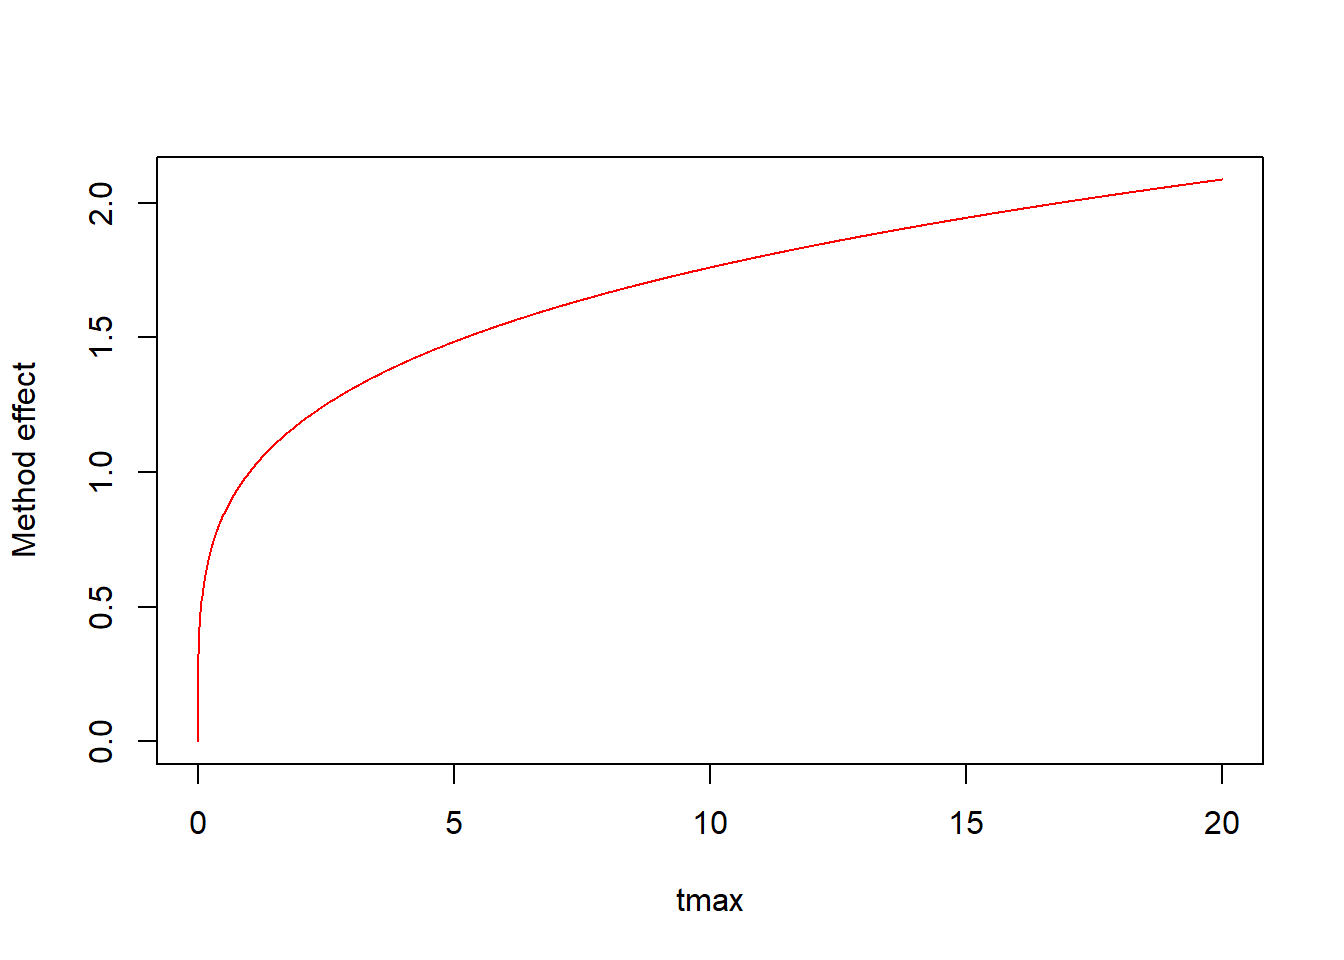
\includegraphics{qpad-book_files/figure-latex/regr-time8-1.pdf}

Now we are getting somewhere. But still, this function keep
increasing monotonically.

\BeginKnitrBlock{rmdexercise}
\textbf{Exercise}

What kind of function would we need and why?

What is the underlying biological mechanism?
\EndKnitrBlock{rmdexercise}

\hypertarget{count-radius-effects}{%
\section{Count radius effects}\label{count-radius-effects}}

Before solving the count duration issue, let us look at the
effect of survey area.
We get a similar count breakdown, but now by distance band:

\begin{Shaded}
\begin{Highlighting}[]
\NormalTok{ydis <-}\StringTok{ }\KeywordTok{Xtab}\NormalTok{(}\OperatorTok{~}\StringTok{ }\NormalTok{SiteID }\OperatorTok{+}\StringTok{ }\NormalTok{Dis }\OperatorTok{+}\StringTok{ }\NormalTok{SpeciesID , }
\NormalTok{  josm}\OperatorTok{$}\NormalTok{counts[josm}\OperatorTok{$}\NormalTok{counts}\OperatorTok{$}\NormalTok{DetectType1 }\OperatorTok{!=}\StringTok{ "V"}\NormalTok{,])}

\NormalTok{y <-}\StringTok{ }\KeywordTok{as.matrix}\NormalTok{(ydis[[spp]])}
\KeywordTok{head}\NormalTok{(y)}
\end{Highlighting}
\end{Shaded}

\begin{verbatim}
##         0-50m 50-100m 100+m
## CL10102     1       2     0
## CL10106     0       0     0
## CL10108     0       0     0
## CL10109     1       2     0
## CL10111     1       0     1
## CL10112     0       2     0
\end{verbatim}

\begin{Shaded}
\begin{Highlighting}[]
\KeywordTok{colMeans}\NormalTok{(y) }\CommentTok{# mean count of new individuals}
\end{Highlighting}
\end{Shaded}

\begin{verbatim}
##   0-50m 50-100m   100+m 
## 0.29241 0.49223 0.09849
\end{verbatim}

\begin{Shaded}
\begin{Highlighting}[]
\KeywordTok{cumsum}\NormalTok{(}\KeywordTok{colMeans}\NormalTok{(y)) }\CommentTok{# cumulative counts}
\end{Highlighting}
\end{Shaded}

\begin{verbatim}
##   0-50m 50-100m   100+m 
##  0.2924  0.7846  0.8831
\end{verbatim}

\begin{Shaded}
\begin{Highlighting}[]
\NormalTok{x <-}\StringTok{ }\KeywordTok{data.frame}\NormalTok{(}
\NormalTok{  josm}\OperatorTok{$}\NormalTok{surveys, }
  \DataTypeTok{y50=}\NormalTok{y[,}\StringTok{"0-50m"}\NormalTok{],}
  \DataTypeTok{y100=}\NormalTok{y[,}\StringTok{"0-50m"}\NormalTok{]}\OperatorTok{+}\NormalTok{y[,}\StringTok{"50-100m"}\NormalTok{])}

\KeywordTok{table}\NormalTok{(x}\OperatorTok{$}\NormalTok{y50)}
\end{Highlighting}
\end{Shaded}

\begin{verbatim}
## 
##    0    1    2    3    4    5 
## 3521  792  228   25    2    1
\end{verbatim}

\begin{Shaded}
\begin{Highlighting}[]
\KeywordTok{table}\NormalTok{(x}\OperatorTok{$}\NormalTok{y100)}
\end{Highlighting}
\end{Shaded}

\begin{verbatim}
## 
##    0    1    2    3    4    5    6 
## 2654  833  647  316   92   20    7
\end{verbatim}

We don't consider the unlimited distance case, because the survey area there
is unknown (although we will ultimately address this problem mater).
We compare the counts within the 0-50 and 0-100 m circles:

\begin{Shaded}
\begin{Highlighting}[]
\NormalTok{m50 <-}\StringTok{ }\KeywordTok{glm}\NormalTok{(y50 }\OperatorTok{~}\StringTok{ }\NormalTok{Decid, }\DataTypeTok{data=}\NormalTok{x, }\DataTypeTok{family=}\NormalTok{poisson)}
\NormalTok{m100 <-}\StringTok{ }\KeywordTok{glm}\NormalTok{(y100 }\OperatorTok{~}\StringTok{ }\NormalTok{Decid, }\DataTypeTok{data=}\NormalTok{x, }\DataTypeTok{family=}\NormalTok{poisson)}
\KeywordTok{mean}\NormalTok{(}\KeywordTok{fitted}\NormalTok{(m50))}
\end{Highlighting}
\end{Shaded}

\begin{verbatim}
## [1] 0.2924
\end{verbatim}

\begin{Shaded}
\begin{Highlighting}[]
\KeywordTok{mean}\NormalTok{(}\KeywordTok{fitted}\NormalTok{(m100))}
\end{Highlighting}
\end{Shaded}

\begin{verbatim}
## [1] 0.7846
\end{verbatim}

\begin{Shaded}
\begin{Highlighting}[]
\KeywordTok{coef}\NormalTok{(m50)}
\end{Highlighting}
\end{Shaded}

\begin{verbatim}
## (Intercept)       Decid 
##      -2.265       2.126
\end{verbatim}

\begin{Shaded}
\begin{Highlighting}[]
\KeywordTok{coef}\NormalTok{(m100)}
\end{Highlighting}
\end{Shaded}

\begin{verbatim}
## (Intercept)       Decid 
##      -1.327       2.209
\end{verbatim}

\hypertarget{offsets}{%
\section{Offsets}\label{offsets}}

Offsets are constant terms in the linear predictor,
e.g.~\(log(\lambda_i) = \beta_0 + \beta_1 x_{1i} + o_i\),
where \(o_i\) is an offset. In the survey area case,
an offset might be the log of area surveyed.
The logic for this is based on point processes:
intensity is a linear function of area
under a homogeneous Poisson point process.
So we can assume that \(o_i = log(A_i)\), where \(A\) stands for area.

Let's see if using area as offset makes our models comparable:

\begin{Shaded}
\begin{Highlighting}[]
\NormalTok{m50 <-}\StringTok{ }\KeywordTok{glm}\NormalTok{(y50 }\OperatorTok{~}\StringTok{ }\NormalTok{Decid, }\DataTypeTok{data=}\NormalTok{x, }\DataTypeTok{family=}\NormalTok{poisson, }
  \DataTypeTok{offset=}\KeywordTok{rep}\NormalTok{(}\KeywordTok{log}\NormalTok{(}\FloatTok{0.5}\OperatorTok{^}\DecValTok{2}\OperatorTok{*}\NormalTok{pi), }\KeywordTok{nrow}\NormalTok{(x)))}
\NormalTok{m100 <-}\StringTok{ }\KeywordTok{glm}\NormalTok{(y100 }\OperatorTok{~}\StringTok{ }\NormalTok{Decid, }\DataTypeTok{data=}\NormalTok{x, }\DataTypeTok{family=}\NormalTok{poisson,}
  \DataTypeTok{offset=}\KeywordTok{rep}\NormalTok{(}\KeywordTok{log}\NormalTok{(}\DecValTok{1}\OperatorTok{^}\DecValTok{2}\OperatorTok{*}\NormalTok{pi), }\KeywordTok{nrow}\NormalTok{(x)))}
\KeywordTok{coef}\NormalTok{(m50)}
\end{Highlighting}
\end{Shaded}

\begin{verbatim}
## (Intercept)       Decid 
##      -2.024       2.126
\end{verbatim}

\begin{Shaded}
\begin{Highlighting}[]
\KeywordTok{coef}\NormalTok{(m100)}
\end{Highlighting}
\end{Shaded}

\begin{verbatim}
## (Intercept)       Decid 
##      -2.471       2.209
\end{verbatim}

\begin{Shaded}
\begin{Highlighting}[]
\KeywordTok{mean}\NormalTok{(}\KeywordTok{exp}\NormalTok{(}\KeywordTok{model.matrix}\NormalTok{(m50) }\OperatorTok\StringTok{ }\KeywordTok{coef}\NormalTok{(m50)))}
\end{Highlighting}
\end{Shaded}

\begin{verbatim}
## [1] 0.3723
\end{verbatim}

\begin{Shaded}
\begin{Highlighting}[]
\KeywordTok{mean}\NormalTok{(}\KeywordTok{exp}\NormalTok{(}\KeywordTok{model.matrix}\NormalTok{(m100) }\OperatorTok\StringTok{ }\KeywordTok{coef}\NormalTok{(m100)))}
\end{Highlighting}
\end{Shaded}

\begin{verbatim}
## [1] 0.2498
\end{verbatim}

These coefficients and mean predictions are much closer to each other,
but something else is going on.

\BeginKnitrBlock{rmdexercise}
\textbf{Exercise}

Can you guess why we cannot make abundances comparable using
log area as as offset?
\EndKnitrBlock{rmdexercise}

We pretend again, that survey area varies in our data set:

\begin{Shaded}
\begin{Highlighting}[]
\KeywordTok{set.seed}\NormalTok{(}\DecValTok{1}\NormalTok{)}
\NormalTok{x}\OperatorTok{$}\NormalTok{meth <-}\StringTok{ }\KeywordTok{as.factor}\NormalTok{(}\KeywordTok{sample}\NormalTok{(}\KeywordTok{c}\NormalTok{(}\StringTok{"A"}\NormalTok{, }\StringTok{"B"}\NormalTok{), }\KeywordTok{nrow}\NormalTok{(x), }\DataTypeTok{replace=}\OtherTok{TRUE}\NormalTok{))}
\NormalTok{x}\OperatorTok{$}\NormalTok{y <-}\StringTok{ }\NormalTok{x}\OperatorTok{$}\NormalTok{y50}
\NormalTok{x}\OperatorTok{$}\NormalTok{y[x}\OperatorTok{$}\NormalTok{meth }\OperatorTok{==}\StringTok{ "B"}\NormalTok{] <-}\StringTok{ }\NormalTok{x}\OperatorTok{$}\NormalTok{y100[x}\OperatorTok{$}\NormalTok{meth }\OperatorTok{==}\StringTok{ "B"}\NormalTok{]}
\KeywordTok{boxplot}\NormalTok{(y }\OperatorTok{~}\StringTok{ }\NormalTok{meth, x)}
\end{Highlighting}
\end{Shaded}

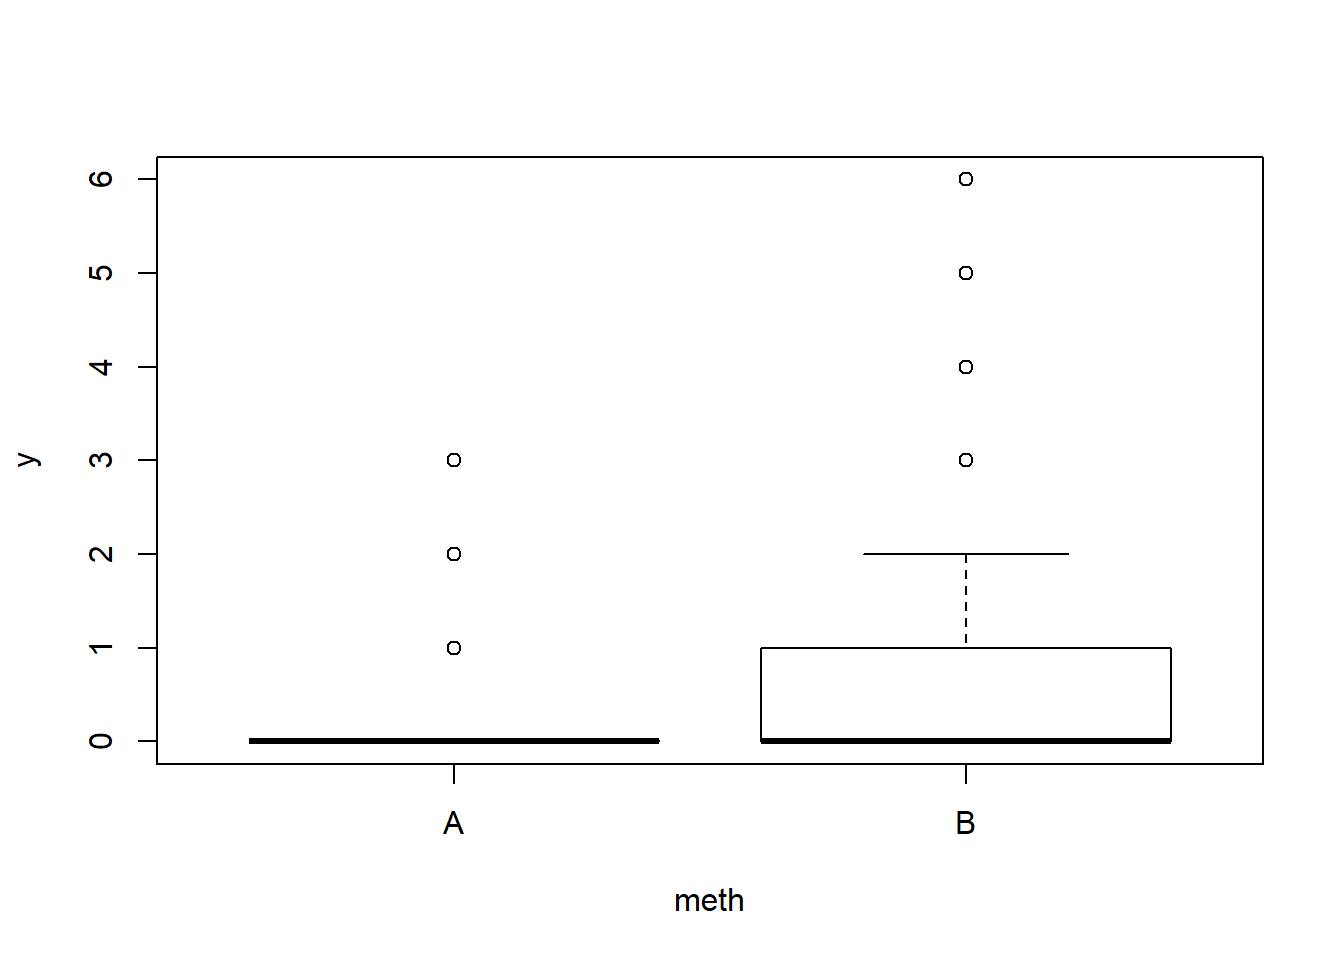
\includegraphics{qpad-book_files/figure-latex/regr-area4-1.pdf}

Methodology effect:

\begin{Shaded}
\begin{Highlighting}[]
\NormalTok{mm <-}\StringTok{ }\KeywordTok{glm}\NormalTok{(y }\OperatorTok{~}\StringTok{ }\NormalTok{meth }\OperatorTok{-}\StringTok{ }\DecValTok{1}\NormalTok{, }\DataTypeTok{data=}\NormalTok{x, }\DataTypeTok{family=}\NormalTok{poisson)}
\KeywordTok{summary}\NormalTok{(mm)}
\end{Highlighting}
\end{Shaded}

\begin{verbatim}
## 
## Call:
## glm(formula = y ~ meth - 1, family = poisson, data = x)
## 
## Deviance Residuals: 
##    Min      1Q  Median      3Q     Max  
## -1.261  -1.261  -0.759   0.221   3.720  
## 
## Coefficients:
##       Estimate Std. Error z value Pr(>|z|)    
## methA  -1.2444     0.0392  -31.77   <2e-16 ***
## methB  -0.2290     0.0234   -9.81   <2e-16 ***
## ---
## Signif. codes:  0 '***' 0.001 '**' 0.01 '*' 0.05 '.' 0.1 ' ' 1
## 
## (Dispersion parameter for poisson family taken to be 1)
## 
##     Null deviance: 7387.0  on 4569  degrees of freedom
## Residual deviance: 5683.8  on 4567  degrees of freedom
## AIC: 9171
## 
## Number of Fisher Scoring iterations: 6
\end{verbatim}

\begin{Shaded}
\begin{Highlighting}[]
\KeywordTok{exp}\NormalTok{(}\KeywordTok{coef}\NormalTok{(mm))}
\end{Highlighting}
\end{Shaded}

\begin{verbatim}
##  methA  methB 
## 0.2881 0.7953
\end{verbatim}

Predictor and method effects:

\begin{Shaded}
\begin{Highlighting}[]
\NormalTok{mm <-}\StringTok{ }\KeywordTok{glm}\NormalTok{(y }\OperatorTok{~}\StringTok{ }\NormalTok{Decid }\OperatorTok{+}\StringTok{ }\NormalTok{meth, }\DataTypeTok{data=}\NormalTok{x, }\DataTypeTok{family=}\NormalTok{poisson)}
\KeywordTok{summary}\NormalTok{(mm)}
\end{Highlighting}
\end{Shaded}

\begin{verbatim}
## 
## Call:
## glm(formula = y ~ Decid + meth, family = poisson, data = x)
## 
## Deviance Residuals: 
##    Min      1Q  Median      3Q     Max  
## -2.209  -0.855  -0.589   0.244   3.577  
## 
## Coefficients:
##             Estimate Std. Error z value Pr(>|z|)    
## (Intercept)  -2.3275     0.0567   -41.0   <2e-16 ***
## Decid         2.1961     0.0689    31.9   <2e-16 ***
## methB         1.0284     0.0456    22.6   <2e-16 ***
## ---
## Signif. codes:  0 '***' 0.001 '**' 0.01 '*' 0.05 '.' 0.1 ' ' 1
## 
## (Dispersion parameter for poisson family taken to be 1)
## 
##     Null deviance: 6247.1  on 4568  degrees of freedom
## Residual deviance: 4595.6  on 4566  degrees of freedom
## AIC: 8085
## 
## Number of Fisher Scoring iterations: 6
\end{verbatim}

\begin{Shaded}
\begin{Highlighting}[]
\KeywordTok{boxplot}\NormalTok{(}\KeywordTok{fitted}\NormalTok{(mm) }\OperatorTok{~}\StringTok{ }\NormalTok{meth, x)}
\end{Highlighting}
\end{Shaded}

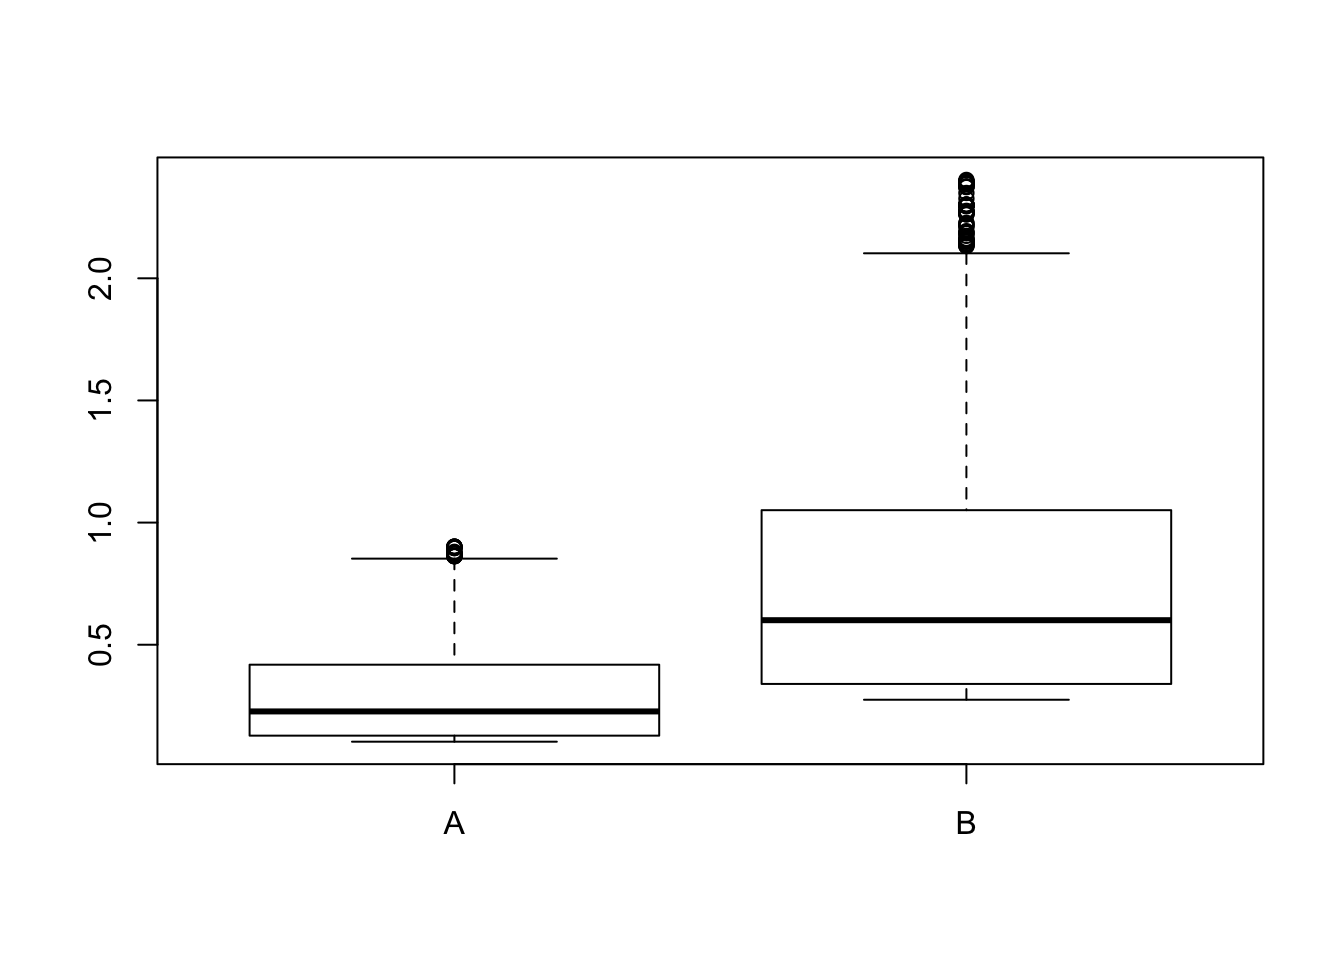
\includegraphics{qpad-book_files/figure-latex/regr-area6-1.pdf}

\begin{Shaded}
\begin{Highlighting}[]
\KeywordTok{exp}\NormalTok{(}\KeywordTok{coef}\NormalTok{(mm))}
\end{Highlighting}
\end{Shaded}

\begin{verbatim}
## (Intercept)       Decid       methB 
##     0.09754     8.98996     2.79646
\end{verbatim}

\begin{Shaded}
\begin{Highlighting}[]
\KeywordTok{cumsum}\NormalTok{(}\KeywordTok{colMeans}\NormalTok{(y))[}\DecValTok{1}\OperatorTok{:}\DecValTok{2}\NormalTok{]}
\end{Highlighting}
\end{Shaded}

\begin{verbatim}
##   0-50m 50-100m 
##  0.2924  0.7846
\end{verbatim}

\begin{Shaded}
\begin{Highlighting}[]
\KeywordTok{mean}\NormalTok{(y[,}\DecValTok{1}\NormalTok{]) }\OperatorTok{*}\StringTok{ }\KeywordTok{c}\NormalTok{(}\DecValTok{1}\NormalTok{, }\KeywordTok{exp}\NormalTok{(}\KeywordTok{coef}\NormalTok{(mm))[}\DecValTok{3}\NormalTok{])}
\end{Highlighting}
\end{Shaded}

\begin{verbatim}
##         methB 
## 0.2924 0.8177
\end{verbatim}

Use log area as continuous predictor:
we would expect a close to 1:1 relationship on the
abundance scale.

\begin{Shaded}
\begin{Highlighting}[]
\NormalTok{x}\OperatorTok{$}\NormalTok{logA <-}\StringTok{ }\KeywordTok{log}\NormalTok{(}\KeywordTok{ifelse}\NormalTok{(x}\OperatorTok{$}\NormalTok{meth }\OperatorTok{==}\StringTok{ "A"}\NormalTok{, }\FloatTok{0.5}\NormalTok{, }\DecValTok{1}\NormalTok{)}\OperatorTok{^}\DecValTok{2}\OperatorTok{*}\NormalTok{pi)}
\NormalTok{mm <-}\StringTok{ }\KeywordTok{glm}\NormalTok{(y }\OperatorTok{~}\StringTok{ }\NormalTok{Decid }\OperatorTok{+}\StringTok{ }\NormalTok{logA, }\DataTypeTok{data=}\NormalTok{x, }\DataTypeTok{family=}\NormalTok{poisson)}
\KeywordTok{summary}\NormalTok{(mm)}
\end{Highlighting}
\end{Shaded}

\begin{verbatim}
## 
## Call:
## glm(formula = y ~ Decid + logA, family = poisson, data = x)
## 
## Deviance Residuals: 
##    Min      1Q  Median      3Q     Max  
## -2.209  -0.855  -0.589   0.244   3.577  
## 
## Coefficients:
##             Estimate Std. Error z value Pr(>|z|)    
## (Intercept)  -2.1483     0.0523   -41.1   <2e-16 ***
## Decid         2.1961     0.0689    31.9   <2e-16 ***
## logA          0.7418     0.0329    22.6   <2e-16 ***
## ---
## Signif. codes:  0 '***' 0.001 '**' 0.01 '*' 0.05 '.' 0.1 ' ' 1
## 
## (Dispersion parameter for poisson family taken to be 1)
## 
##     Null deviance: 6247.1  on 4568  degrees of freedom
## Residual deviance: 4595.6  on 4566  degrees of freedom
## AIC: 8085
## 
## Number of Fisher Scoring iterations: 6
\end{verbatim}

\begin{Shaded}
\begin{Highlighting}[]
\NormalTok{A <-}\StringTok{ }\KeywordTok{seq}\NormalTok{(}\DecValTok{0}\NormalTok{, }\DecValTok{2}\NormalTok{, }\FloatTok{0.01}\NormalTok{) }\CommentTok{# in ha}
\KeywordTok{plot}\NormalTok{(A, }\KeywordTok{exp}\NormalTok{(}\KeywordTok{log}\NormalTok{(A) }\OperatorTok{*}\StringTok{ }\KeywordTok{coef}\NormalTok{(mm)[}\DecValTok{3}\NormalTok{]), }\DataTypeTok{type=}\StringTok{"l"}\NormalTok{,}
  \DataTypeTok{ylab=}\StringTok{"Method effect"}\NormalTok{, }\DataTypeTok{col=}\DecValTok{2}\NormalTok{)}
\KeywordTok{abline}\NormalTok{(}\DecValTok{0}\NormalTok{, }\DecValTok{1}\NormalTok{, }\DataTypeTok{lty=}\DecValTok{2}\NormalTok{)}
\end{Highlighting}
\end{Shaded}

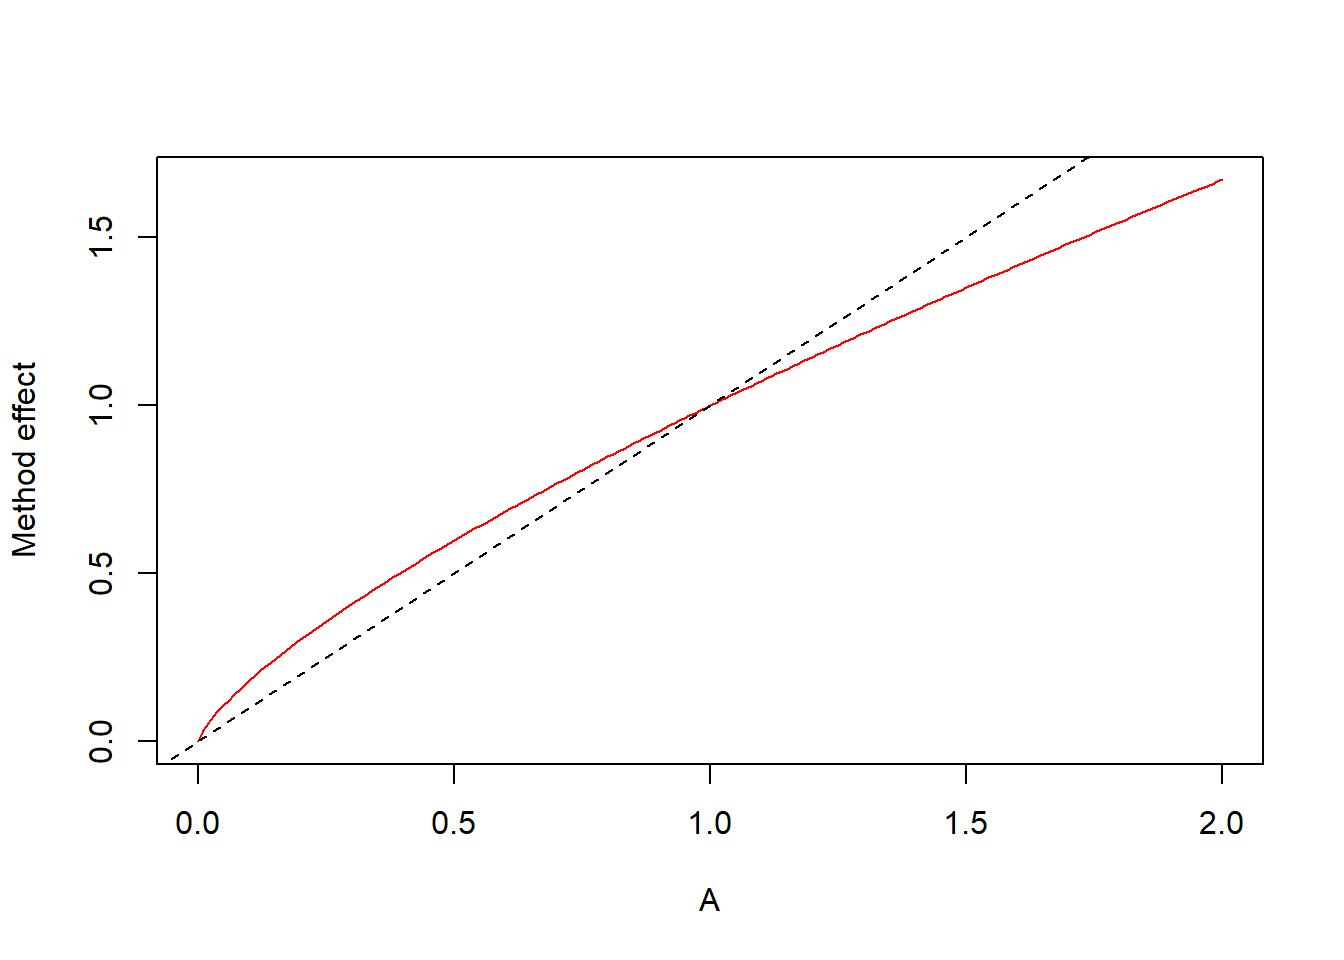
\includegraphics{qpad-book_files/figure-latex/regr-area7-1.pdf}

The offset forces the relationship to be 1:1
(it is like fixing the \texttt{logA} coefficient to be 1):

\begin{Shaded}
\begin{Highlighting}[]
\NormalTok{mm <-}\StringTok{ }\KeywordTok{glm}\NormalTok{(y }\OperatorTok{~}\StringTok{ }\NormalTok{Decid, }\DataTypeTok{data=}\NormalTok{x, }\DataTypeTok{family=}\NormalTok{poisson, }\DataTypeTok{offset=}\NormalTok{x}\OperatorTok{$}\NormalTok{logA)}
\KeywordTok{summary}\NormalTok{(mm)}
\end{Highlighting}
\end{Shaded}

\begin{verbatim}
## 
## Call:
## glm(formula = y ~ Decid, family = poisson, data = x, offset = x$logA)
## 
## Deviance Residuals: 
##    Min      1Q  Median      3Q     Max  
## -2.305  -0.842  -0.525   0.234   3.600  
## 
## Coefficients:
##             Estimate Std. Error z value Pr(>|z|)    
## (Intercept)  -2.3658     0.0453   -52.2   <2e-16 ***
## Decid         2.2031     0.0690    31.9   <2e-16 ***
## ---
## Signif. codes:  0 '***' 0.001 '**' 0.01 '*' 0.05 '.' 0.1 ' ' 1
## 
## (Dispersion parameter for poisson family taken to be 1)
## 
##     Null deviance: 5746.0  on 4568  degrees of freedom
## Residual deviance: 4653.6  on 4567  degrees of freedom
## AIC: 8141
## 
## Number of Fisher Scoring iterations: 6
\end{verbatim}

\begin{Shaded}
\begin{Highlighting}[]
\KeywordTok{boxplot}\NormalTok{(}\KeywordTok{fitted}\NormalTok{(mm) }\OperatorTok{~}\StringTok{ }\NormalTok{meth, x)}
\end{Highlighting}
\end{Shaded}

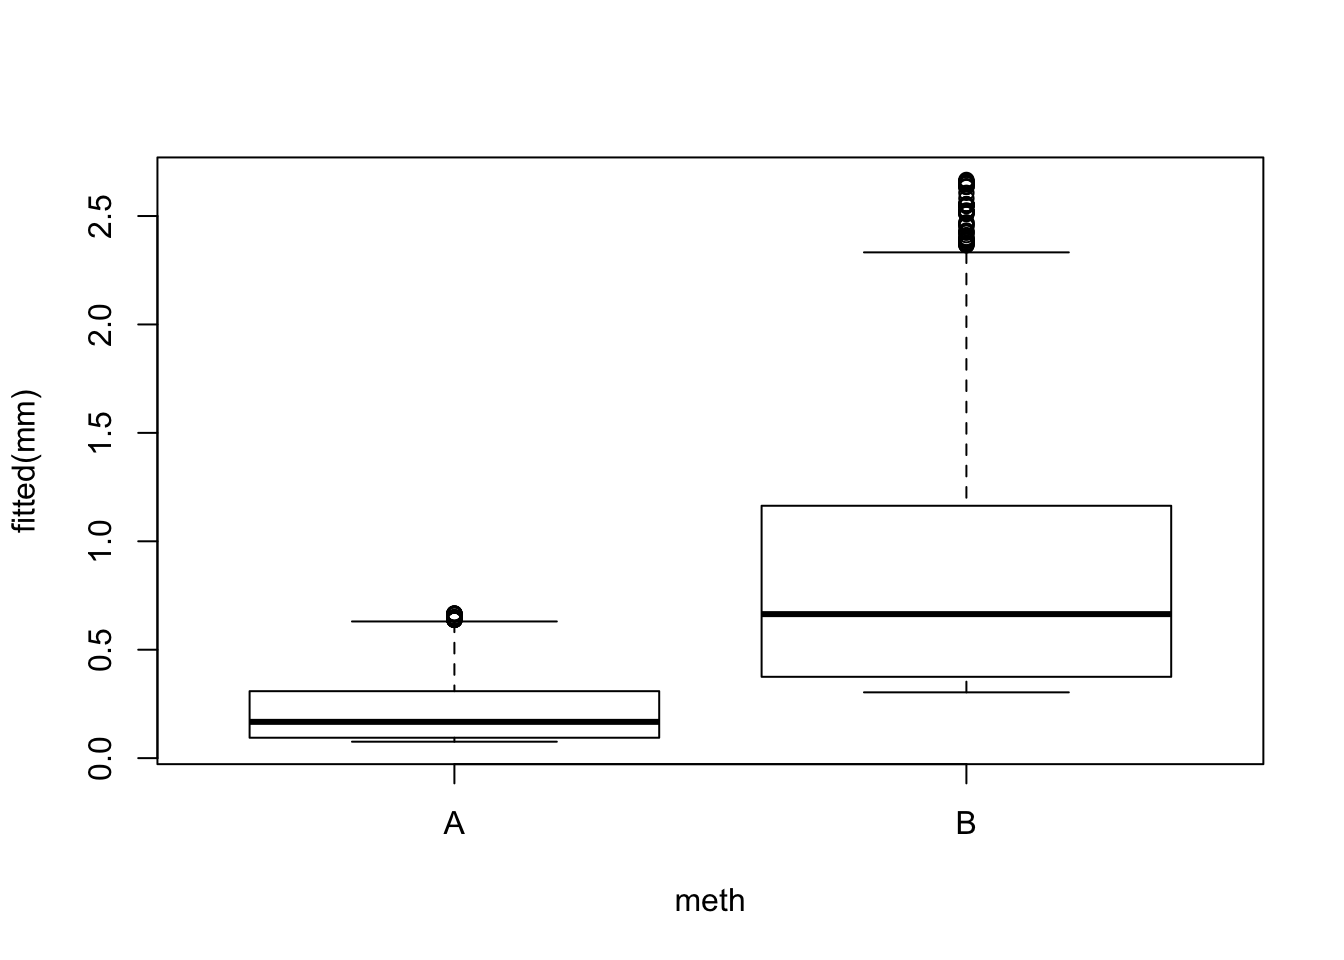
\includegraphics{qpad-book_files/figure-latex/regr-area8-1.pdf}

\begin{Shaded}
\begin{Highlighting}[]
\KeywordTok{cumsum}\NormalTok{(}\KeywordTok{colMeans}\NormalTok{(y))[}\DecValTok{1}\OperatorTok{:}\DecValTok{2}\NormalTok{]}
\end{Highlighting}
\end{Shaded}

\begin{verbatim}
##   0-50m 50-100m 
##  0.2924  0.7846
\end{verbatim}

\begin{Shaded}
\begin{Highlighting}[]
\KeywordTok{c}\NormalTok{(}\FloatTok{0.5}\NormalTok{, }\DecValTok{1}\NormalTok{)}\OperatorTok{^}\DecValTok{2}\OperatorTok{*}\NormalTok{pi }\OperatorTok{*}\StringTok{ }\KeywordTok{mean}\NormalTok{(}\KeywordTok{exp}\NormalTok{(}\KeywordTok{model.matrix}\NormalTok{(mm) }\OperatorTok\StringTok{ }\KeywordTok{coef}\NormalTok{(mm))) }\CommentTok{# /ha}
\end{Highlighting}
\end{Shaded}

\begin{verbatim}
## [1] 0.2173 0.8691
\end{verbatim}

\BeginKnitrBlock{rmdexercise}
\textbf{Exercise}

Why did we get a \texttt{logA} coefficient that was less than 1 when theoretically we should have gotten 1?
\EndKnitrBlock{rmdexercise}

Predictions using offsets in \texttt{glm} can be tricky.
The safest way is to use the matrix product
(\texttt{exp(model.matrix(mm)\ \%*\%\ coef(mm)\ +\ \textless{}offset\textgreater{})}).
We can often omit the offset, e.g.~in the log area case
we can express the prediction per unit area.
If the unit is 1 ha, as in our case, log(1)=0, which means
the mean abundance per unit area can be calculated by
omitting the offsets all together.

\hypertarget{behavior}{%
\chapter{Behavioral Complexities}\label{behavior}}

\hypertarget{introduction-2}{%
\section{Introduction}\label{introduction-2}}

We have reviewed so far how to fit \emph{naive} models to estimate
the expected value of the observed counts, \(\lambda\).
So what is this \(\lambda\)?
Here are some deifinitions for further discussion:

\begin{itemize}
\tightlist
\item
  \textbf{relative abundance}: \(\lambda\) without any reference to nuisance variables, but possibly standardized by design, or nuisance variables used as fixed effects,
\item
  \textbf{abundance}: \(N=\lambda/C\), \(C\) is a correction factor and \(N\) refers to the number of individuals within the area surveyed -- the problem is that we cannot measure this directly (this is a latent variable), moreover the survey area is also often unknown (i.e.~for unlimited distance counts),
\item
  \textbf{occupancy}: the probability that the survey area is occupied, this is really equivalent to the indicator function \(N>0\),
\item
  \textbf{density} \(D = N/A = \lambda/AC\), abundance per unit area -- same problems as above: both \(N\) and \(A\) are unknowns.
\end{itemize}

Our objective in the following chapters is to work out the details of
estimating abundance and density in some clever ways through
learning about the nature of the mechanisms contributing to \(C\).

\hypertarget{prerequisites-2}{%
\section{Prerequisites}\label{prerequisites-2}}

\begin{Shaded}
\begin{Highlighting}[]
\KeywordTok{library}\NormalTok{(bSims)                }\CommentTok{# simulations}
\KeywordTok{library}\NormalTok{(detect)               }\CommentTok{# multinomial models}
\KeywordTok{load}\NormalTok{(}\StringTok{"_data/josm/josm.rda"}\NormalTok{) }\CommentTok{# JOSM data}
\end{Highlighting}
\end{Shaded}

\hypertarget{birds-in-the-forest}{%
\section{Birds in the forest}\label{birds-in-the-forest}}

Build a landscape: extent is given in 100 m units

\begin{Shaded}
\begin{Highlighting}[]
\NormalTok{(l <-}\StringTok{ }\KeywordTok{bsims_init}\NormalTok{(}\DataTypeTok{extent=}\DecValTok{10}\NormalTok{))}
\end{Highlighting}
\end{Shaded}

\begin{verbatim}
## bSims landscape
##   1 km x 1 km
##   stratification: H
\end{verbatim}

\begin{Shaded}
\begin{Highlighting}[]
\KeywordTok{plot}\NormalTok{(l)}
\end{Highlighting}
\end{Shaded}

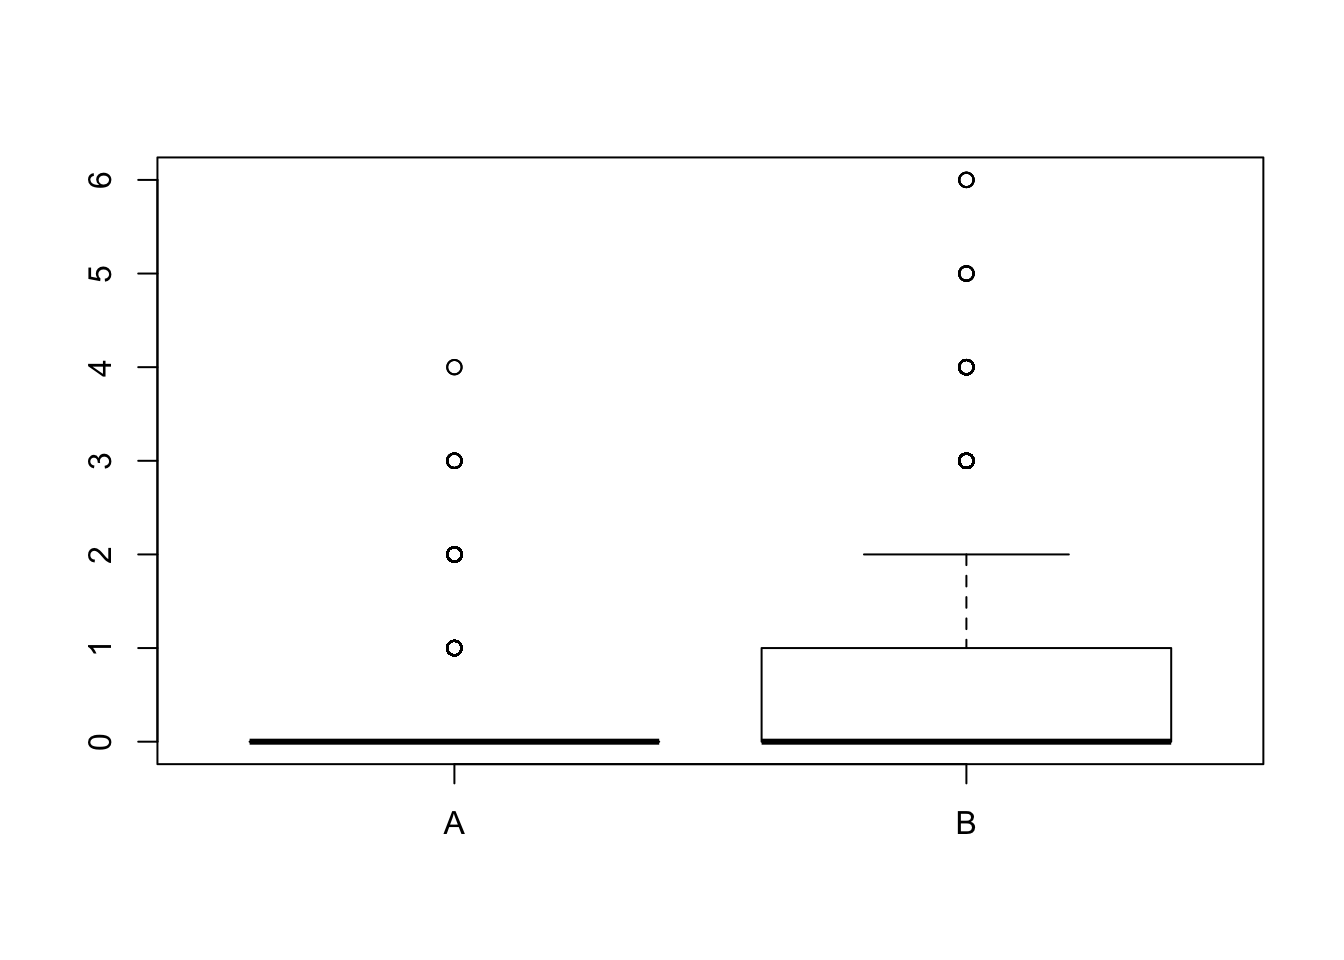
\includegraphics{qpad-book_files/figure-latex/unnamed-chunk-38-1.pdf}

We have a 100 ha landscape that we populate with birds,
1 bird / ha using a Poisson spatial point process.
As a result, we have \(N\) birds in the landscape,
\(N \sim Poisson(\lambda)\), \(\lambda = DA\):

\begin{Shaded}
\begin{Highlighting}[]
\KeywordTok{set.seed}\NormalTok{(}\DecValTok{1}\NormalTok{)}
\NormalTok{(a <-}\StringTok{ }\KeywordTok{bsims_populate}\NormalTok{(l, }\DataTypeTok{density=}\FloatTok{0.5}\NormalTok{))}
\end{Highlighting}
\end{Shaded}

\begin{verbatim}
## bSims population
##   1 km x 1 km
##   stratification: H
##   total abundance: 52
\end{verbatim}

\begin{Shaded}
\begin{Highlighting}[]
\KeywordTok{plot}\NormalTok{(a)}
\end{Highlighting}
\end{Shaded}

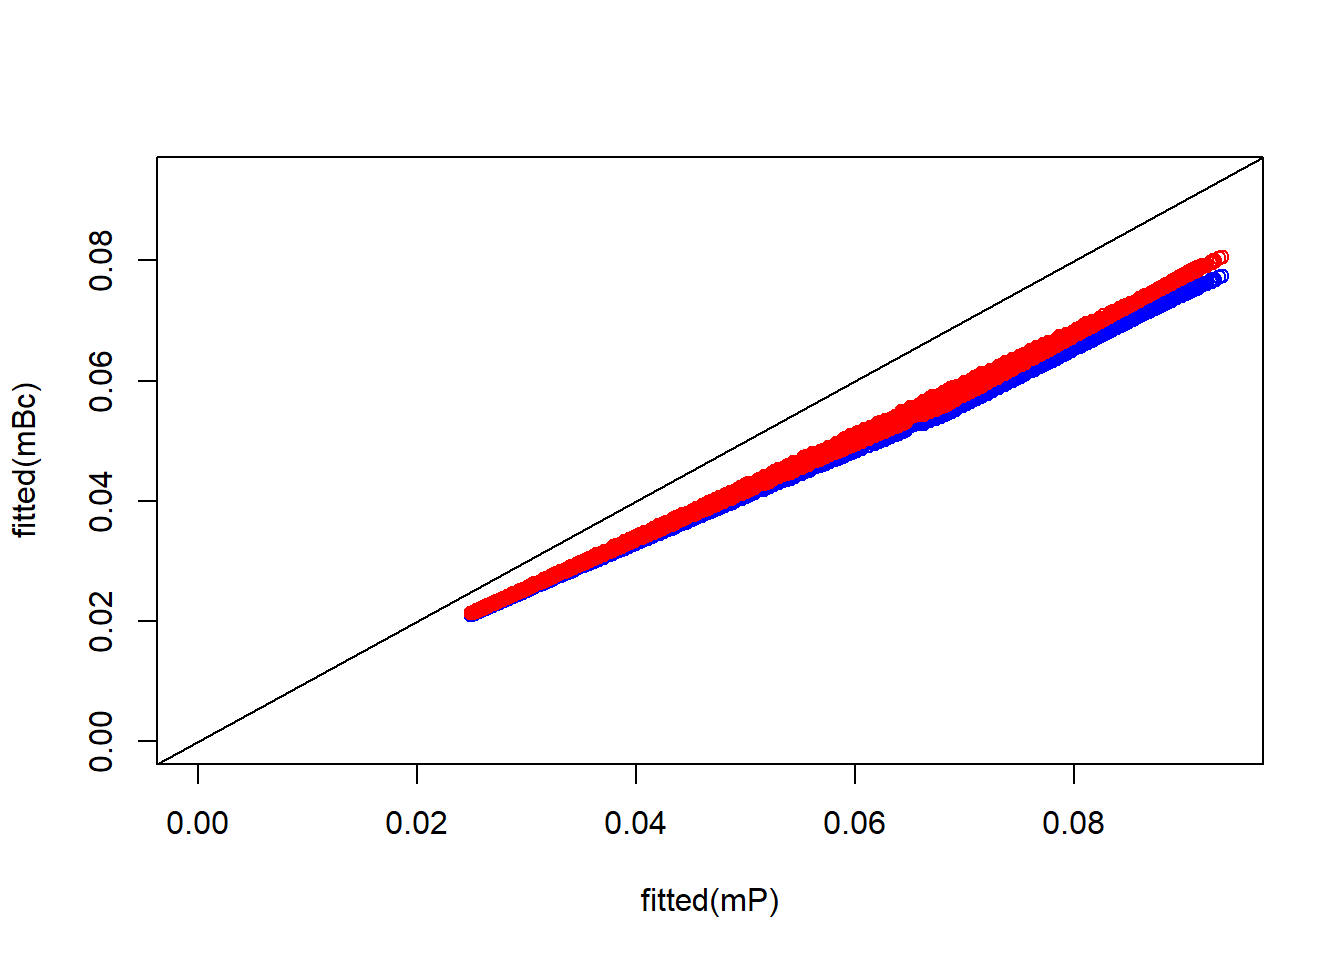
\includegraphics{qpad-book_files/figure-latex/unnamed-chunk-40-1.pdf}

The locations can be seen as nest locations (\texttt{a\$nests} stores the locations).
But birds don't just stay put in one place. They move and vocalize:

\begin{Shaded}
\begin{Highlighting}[]
\NormalTok{(b <-}\StringTok{ }\KeywordTok{bsims_animate}\NormalTok{(a, }
  \DataTypeTok{vocal_rate=}\FloatTok{0.5}\NormalTok{, }\DataTypeTok{duration=}\DecValTok{10}\NormalTok{,}
  \DataTypeTok{move_rate=}\DecValTok{1}\NormalTok{, }\DataTypeTok{movement=}\FloatTok{0.25}\NormalTok{))}
\end{Highlighting}
\end{Shaded}

\begin{verbatim}
## bSims events
##   1 km x 1 km
##   stratification: H
##   total abundance: 52
##   total duration: 10
\end{verbatim}

\begin{Shaded}
\begin{Highlighting}[]
\KeywordTok{plot}\NormalTok{(b)}
\end{Highlighting}
\end{Shaded}

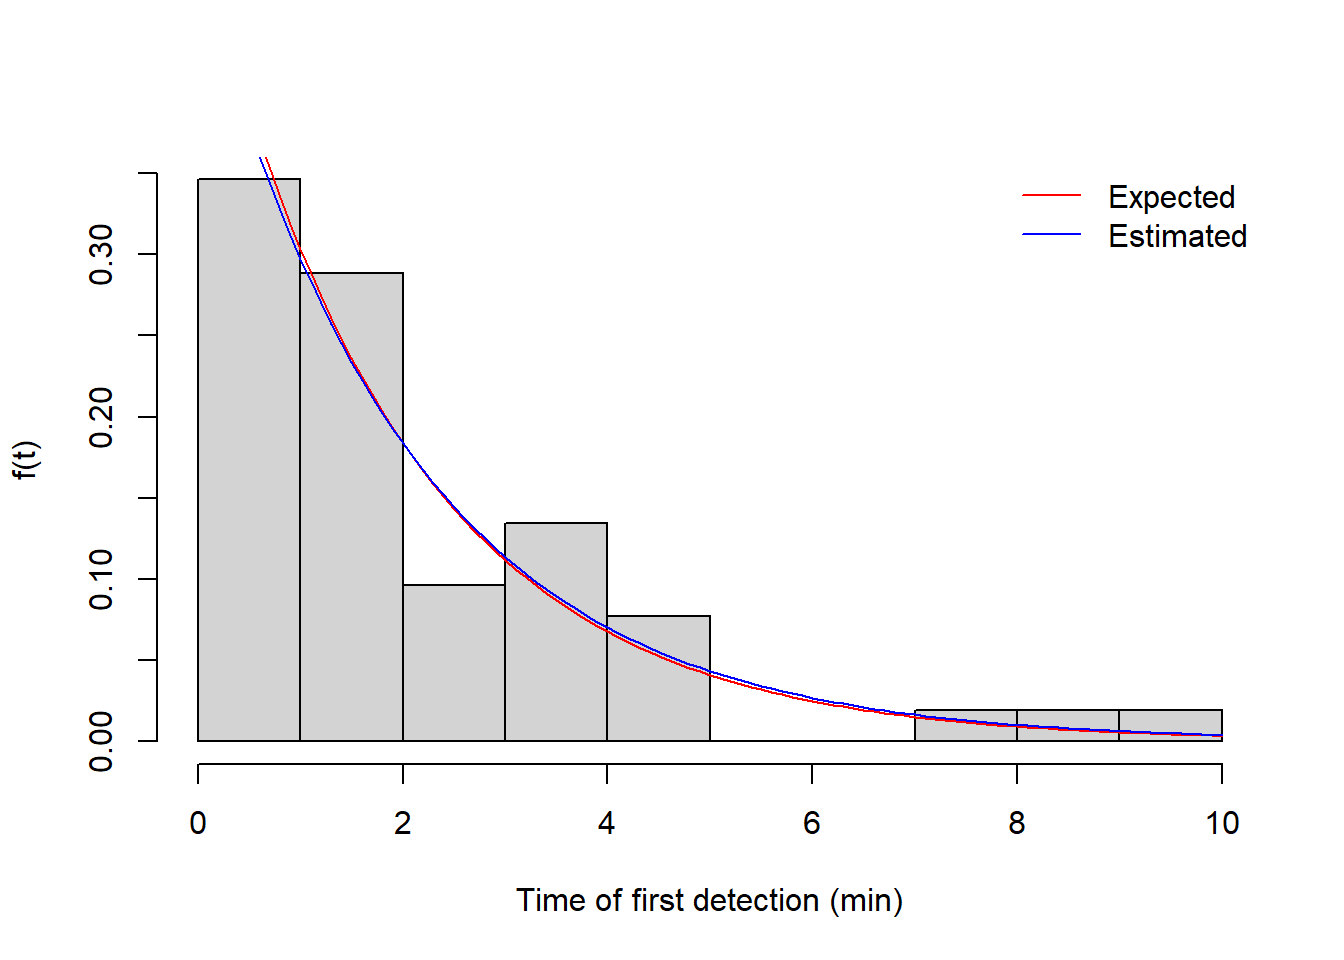
\includegraphics{qpad-book_files/figure-latex/unnamed-chunk-42-1.pdf}

The \texttt{get\_events} function, as the name implies, extracts the events:
movements (\texttt{\$v} is 0) and vocalizations (\texttt{\$v} is 1) alike,
unless filtered for vocalization events only.
Besides the coordinates, we also have the time of event (\texttt{\$t}) and
the individual identifier (\texttt{\$i} linking to the rows of the \texttt{b\$nests} table):

\begin{Shaded}
\begin{Highlighting}[]
\NormalTok{e <-}\StringTok{ }\KeywordTok{get_events}\NormalTok{(b, }\DataTypeTok{vocal_only=}\OtherTok{FALSE}\NormalTok{)}
\KeywordTok{head}\NormalTok{(e)}
\NormalTok{v <-}\StringTok{ }\KeywordTok{get_events}\NormalTok{(b, }\DataTypeTok{vocal_only=}\OtherTok{TRUE}\NormalTok{)}
\KeywordTok{head}\NormalTok{(v)}
\end{Highlighting}
\end{Shaded}

\hypertarget{survival-model}{%
\section{Survival model}\label{survival-model}}

Survival models assess time-to-event data which is often censored
(some event has not occurred at the time the data collection ended).

Event time (\(T\)) is a continuous random variable.
In the simplest case, its probability density function is the Exponential
distribution: \(f(t)=\phi e^{-t\phi}\).
The corresponding cumulative distribution function is:
\(F(t)=\int_{0}^{t} f(t)dt=1-e^{-t\phi}\),
giving the probability that the event has occurred by duration \(t\) and we will refer to
this probability as \(p_t\). The parameter \(\phi\) is the rate of the Exponential distribution
with mean \(1/\phi\) and variance \(1/\phi^2\).

In survival model, the complement of \(F(t)\) is called the
\emph{survival function} (\(S(t)=1-F(t)\), \(S(0)=1\)),
which gives the probability that the event has not occurred by duration \(t\).
The the \emph{hazard function} (\(\lambda(t)=f(t)/S(t)\))
which defines the instantaneous rate of occurrence of the event
(the density of events at \(t\) divided by the probability of surviving).
The cumulative hazard (cumulative risk) the sum of the risks between doration 0 and \(t\)
(\(\Lambda(t)=\int_{0}^{t} \lambda(t)dt\)).

The simplest survival distribution assumes constant risk over time (\(\lambda(t)=\phi\)),
which corresponds to the Exponential distribution.
The Exponential distribution also happens to describe the lengths of the
inter-event times in a homogeneous Poisson process (events are independent, `memory-less' process).

\hypertarget{vocalization-events}{%
\section{Vocalization events}\label{vocalization-events}}

Event times in our bSims example follow a Poisson process with rate \(\phi\) (\texttt{vocal\_rate})
within \texttt{duration} \(t=10\) minutes.

Let's subset the vocalization events to include the time of first detections
for each individual (\texttt{v1}). The estimated rate should match our setting,
the plot shows the Exponential probability density function on top of
the event times:

\begin{Shaded}
\begin{Highlighting}[]
\NormalTok{v1 <-}\StringTok{ }\NormalTok{v[}\OperatorTok{!}\KeywordTok{duplicated}\NormalTok{(v}\OperatorTok{$}\NormalTok{i),]}

\NormalTok{tmp <-}\StringTok{ }\NormalTok{v1}
\NormalTok{tmp}\OperatorTok{$}\NormalTok{o <-}\StringTok{ }\KeywordTok{seq_len}\NormalTok{(}\KeywordTok{nrow}\NormalTok{(v1))}
\KeywordTok{plot}\NormalTok{(o }\OperatorTok{~}\StringTok{ }\NormalTok{t, tmp, }\DataTypeTok{type=}\StringTok{"n"}\NormalTok{, }\DataTypeTok{ylab=}\StringTok{"Individuals"}\NormalTok{,}
  \DataTypeTok{main=}\StringTok{"Vocalization events"}\NormalTok{, }
  \DataTypeTok{ylim=}\KeywordTok{c}\NormalTok{(}\DecValTok{1}\NormalTok{, }\KeywordTok{nrow}\NormalTok{(b}\OperatorTok{$}\NormalTok{nests)), }\DataTypeTok{xlim=}\KeywordTok{c}\NormalTok{(}\DecValTok{0}\NormalTok{,}\DecValTok{10}\NormalTok{))}
\ControlFlowTok{for}\NormalTok{ (i }\ControlFlowTok{in}\NormalTok{ tmp}\OperatorTok{$}\NormalTok{o) \{}
\NormalTok{  tmp2 <-}\StringTok{ }\NormalTok{v[v}\OperatorTok{$}\NormalTok{i }\OperatorTok{==}\StringTok{ }\NormalTok{v1}\OperatorTok{$}\NormalTok{i[i],]}
  \KeywordTok{lines}\NormalTok{(}\KeywordTok{c}\NormalTok{(tmp2}\OperatorTok{$}\NormalTok{t[}\DecValTok{1}\NormalTok{], }\DecValTok{10}\NormalTok{), }\KeywordTok{c}\NormalTok{(i,i), }\DataTypeTok{col=}\StringTok{"grey"}\NormalTok{)}
  \KeywordTok{points}\NormalTok{(tmp2}\OperatorTok{$}\NormalTok{t, }\KeywordTok{rep}\NormalTok{(i, }\KeywordTok{nrow}\NormalTok{(tmp2)), }\DataTypeTok{cex=}\FloatTok{0.5}\NormalTok{)}
  \KeywordTok{points}\NormalTok{(tmp2}\OperatorTok{$}\NormalTok{t[}\DecValTok{1}\NormalTok{], i, }\DataTypeTok{pch=}\DecValTok{19}\NormalTok{, }\DataTypeTok{cex=}\FloatTok{0.5}\NormalTok{)}
\NormalTok{\}}
\end{Highlighting}
\end{Shaded}

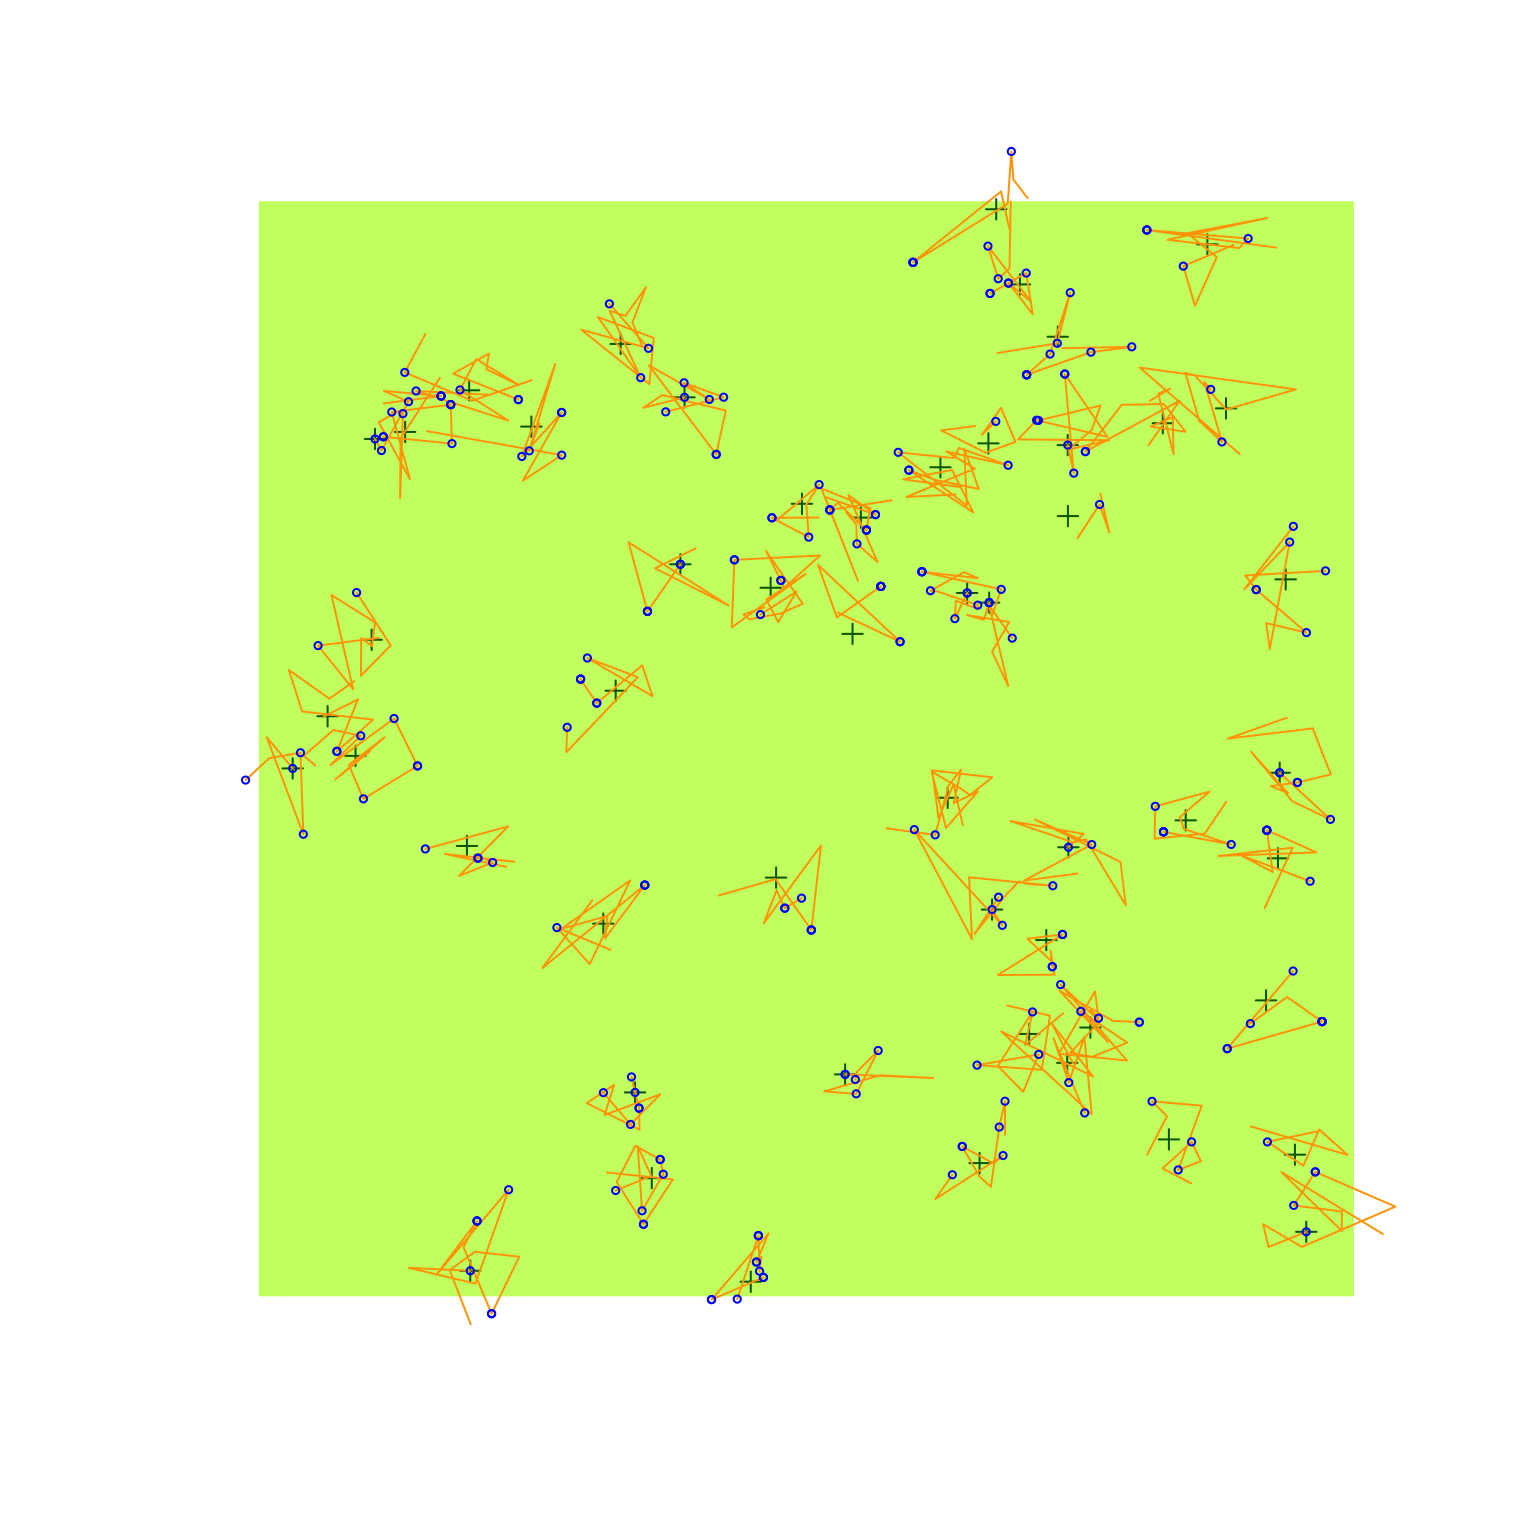
\includegraphics{qpad-book_files/figure-latex/unnamed-chunk-44-1.pdf}

\begin{Shaded}
\begin{Highlighting}[]
\NormalTok{(phi <-}\StringTok{ }\NormalTok{b}\OperatorTok{$}\NormalTok{vocal_rate[}\DecValTok{1}\NormalTok{])}
\end{Highlighting}
\end{Shaded}

\begin{verbatim}
## [1] 0.5
\end{verbatim}

\begin{Shaded}
\begin{Highlighting}[]
\NormalTok{(phi_hat <-}\StringTok{ }\KeywordTok{fitdistr}\NormalTok{(v1}\OperatorTok{$}\NormalTok{t, }\StringTok{"exponential"}\NormalTok{)}\OperatorTok{$}\NormalTok{estimate)}
\end{Highlighting}
\end{Shaded}

\begin{verbatim}
##   rate 
## 0.4808
\end{verbatim}

\begin{Shaded}
\begin{Highlighting}[]
\KeywordTok{hist}\NormalTok{(v1}\OperatorTok{$}\NormalTok{t, }\DataTypeTok{xlab=}\StringTok{"Time of first detection (min)"}\NormalTok{, }\DataTypeTok{freq=}\OtherTok{FALSE}\NormalTok{, }\DataTypeTok{main=}\StringTok{""}\NormalTok{, }
  \DataTypeTok{col=}\StringTok{"lightgrey"}\NormalTok{, }\DataTypeTok{ylab=}\StringTok{"f(t)"}\NormalTok{)}
\KeywordTok{curve}\NormalTok{(}\KeywordTok{dexp}\NormalTok{(x, phi), }\DataTypeTok{add=}\OtherTok{TRUE}\NormalTok{, }\DataTypeTok{col=}\DecValTok{2}\NormalTok{)}
\KeywordTok{curve}\NormalTok{(}\KeywordTok{dexp}\NormalTok{(x, phi_hat), }\DataTypeTok{add=}\OtherTok{TRUE}\NormalTok{, }\DataTypeTok{col=}\DecValTok{4}\NormalTok{)}
\KeywordTok{legend}\NormalTok{(}\StringTok{"topright"}\NormalTok{, }\DataTypeTok{bty=}\StringTok{"n"}\NormalTok{, }\DataTypeTok{lty=}\DecValTok{1}\NormalTok{, }\DataTypeTok{col=}\KeywordTok{c}\NormalTok{(}\DecValTok{2}\NormalTok{,}\DecValTok{4}\NormalTok{), }
  \DataTypeTok{legend=}\KeywordTok{c}\NormalTok{(}\StringTok{"Expected"}\NormalTok{, }\StringTok{"Estimated"}\NormalTok{))}
\end{Highlighting}
\end{Shaded}

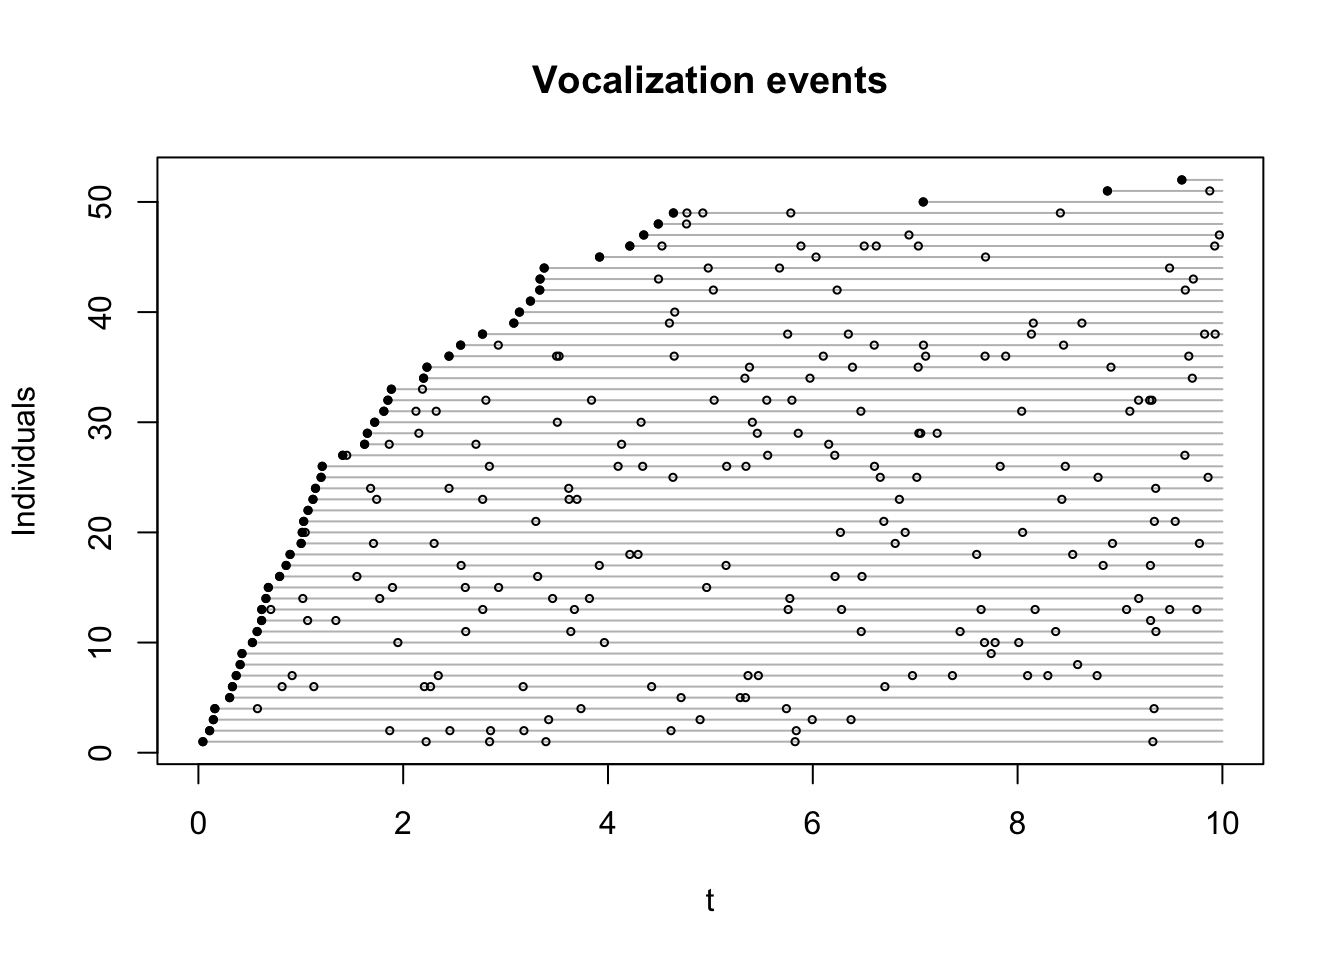
\includegraphics{qpad-book_files/figure-latex/unnamed-chunk-45-1.pdf}

Now let's visualize the corresponding cumulative distribution function.
We also bin the events into time intervals defined by interval end times
in the vector \texttt{br} (breaks to be used with \texttt{cut}):

\begin{Shaded}
\begin{Highlighting}[]
\NormalTok{br <-}\StringTok{ }\KeywordTok{c}\NormalTok{(}\DecValTok{3}\NormalTok{, }\DecValTok{5}\NormalTok{, }\DecValTok{10}\NormalTok{)}
\NormalTok{i <-}\StringTok{ }\KeywordTok{cut}\NormalTok{(v1}\OperatorTok{$}\NormalTok{t, }\KeywordTok{c}\NormalTok{(}\DecValTok{0}\NormalTok{, br), }\DataTypeTok{include.lowest =} \OtherTok{TRUE}\NormalTok{)}
\KeywordTok{table}\NormalTok{(i)}
\end{Highlighting}
\end{Shaded}

\begin{verbatim}
## i
##  [0,3]  (3,5] (5,10] 
##     38     11      3
\end{verbatim}

\begin{Shaded}
\begin{Highlighting}[]
\KeywordTok{plot}\NormalTok{(}\KeywordTok{stepfun}\NormalTok{(v1}\OperatorTok{$}\NormalTok{t, (}\DecValTok{0}\OperatorTok{:}\KeywordTok{nrow}\NormalTok{(v1))}\OperatorTok{/}\KeywordTok{nrow}\NormalTok{(v1)), }\DataTypeTok{do.points=}\OtherTok{FALSE}\NormalTok{, }\DataTypeTok{xlim=}\KeywordTok{c}\NormalTok{(}\DecValTok{0}\NormalTok{,}\DecValTok{10}\NormalTok{),}
  \DataTypeTok{xlab=}\StringTok{"Time of first detection (min)"}\NormalTok{, }\DataTypeTok{ylab=}\StringTok{"F(t)"}\NormalTok{, }\DataTypeTok{main=}\StringTok{""}\NormalTok{)}
\KeywordTok{curve}\NormalTok{(}\DecValTok{1}\OperatorTok{-}\KeywordTok{exp}\NormalTok{(}\OperatorTok{-}\NormalTok{phi}\OperatorTok{*}\NormalTok{x), }\DataTypeTok{add=}\OtherTok{TRUE}\NormalTok{, }\DataTypeTok{col=}\DecValTok{2}\NormalTok{)}
\KeywordTok{curve}\NormalTok{(}\DecValTok{1}\OperatorTok{-}\KeywordTok{exp}\NormalTok{(}\OperatorTok{-}\NormalTok{phi_hat}\OperatorTok{*}\NormalTok{x), }\DataTypeTok{add=}\OtherTok{TRUE}\NormalTok{, }\DataTypeTok{col=}\DecValTok{4}\NormalTok{)}
\KeywordTok{legend}\NormalTok{(}\StringTok{"bottomright"}\NormalTok{, }\DataTypeTok{bty=}\StringTok{"n"}\NormalTok{, }\DataTypeTok{lty=}\KeywordTok{c}\NormalTok{(}\DecValTok{1}\NormalTok{,}\DecValTok{1}\NormalTok{,}\DecValTok{1}\NormalTok{,}\OtherTok{NA}\NormalTok{), }
  \DataTypeTok{col=}\KeywordTok{c}\NormalTok{(}\DecValTok{1}\NormalTok{,}\DecValTok{2}\NormalTok{,}\DecValTok{4}\NormalTok{,}\DecValTok{3}\NormalTok{), }\DataTypeTok{pch=}\KeywordTok{c}\NormalTok{(}\OtherTok{NA}\NormalTok{,}\OtherTok{NA}\NormalTok{,}\OtherTok{NA}\NormalTok{,}\DecValTok{21}\NormalTok{),}
  \DataTypeTok{legend=}\KeywordTok{c}\NormalTok{(}\StringTok{"Empirical"}\NormalTok{, }\StringTok{"Expected"}\NormalTok{, }\StringTok{"Estimated"}\NormalTok{, }\StringTok{"Binned"}\NormalTok{))}
\KeywordTok{points}\NormalTok{(br, }\KeywordTok{cumsum}\NormalTok{(}\KeywordTok{table}\NormalTok{(i))}\OperatorTok{/}\KeywordTok{sum}\NormalTok{(}\KeywordTok{table}\NormalTok{(i)), }\DataTypeTok{cex=}\DecValTok{2}\NormalTok{, }\DataTypeTok{col=}\DecValTok{3}\NormalTok{, }\DataTypeTok{pch=}\DecValTok{21}\NormalTok{)}
\end{Highlighting}
\end{Shaded}

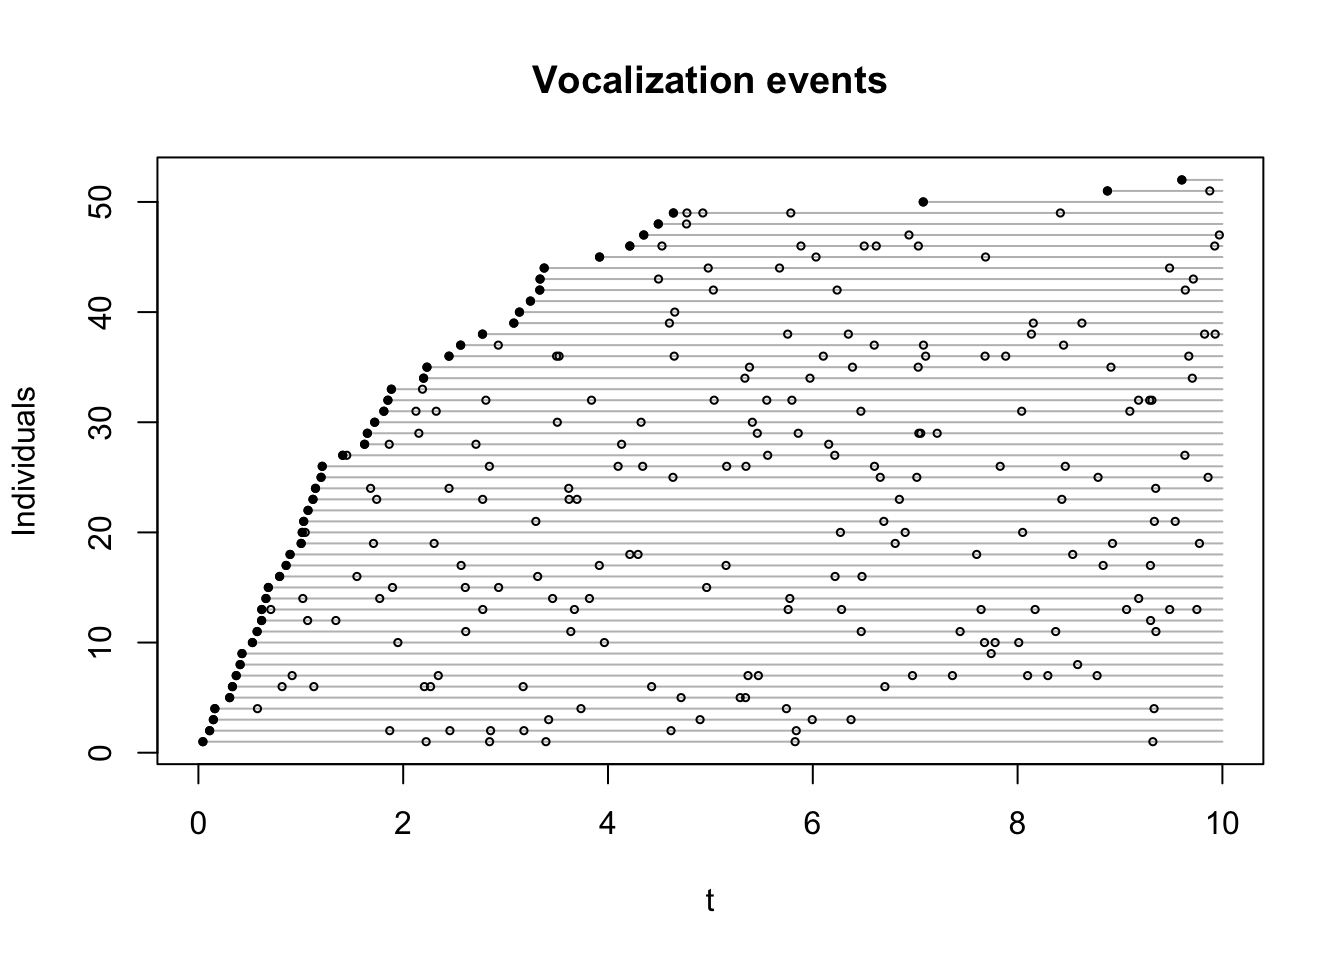
\includegraphics{qpad-book_files/figure-latex/unnamed-chunk-46-1.pdf}

\hypertarget{removal-model}{%
\section{Removal model}\label{removal-model}}

The time-removal model, originally developed for estimating wildlife and fish abundances from mark-recapture studies, was later reformulated for avian surveys with the goal of improving estimates of bird abundance by accounting for the availability bias inherent in point-count data. The removal model applied to point-count surveys estimates the probability that a bird is available for detection as a function of the average number of detectable cues that an individual bird gives per minute (singing rate, \(\phi\)), and the known count duration (\(t\)).

Time-removal models are based on a removal experiment whereby animals are trapped and thereby removed from the closed population of animals being sampled. When applying a removal model to avian point-count surveys, the counts of singing birds (\(Y_{ij}, \ldots, Y_{iJ}\)) within a given point-count survey \(i\) (\(i = 1,\ldots, n\)) are tallied relative to when each bird is first detected in multiple and consecutive time intervals, with the survey start time \(t_{i0} = 0\), the end times of the time intervals \(t_{ij}\) (\(j = 1, 2,\ldots, J\)), and the total count duration of the survey \[t_{iJ}\]. We count each individual bird once, so individuals are `mentally removed' from a closed population of undetected birds by the surveyor.

The continuous-time formulation of the removal model is identical to the Exponential survival model
formulation with respect to the cumulative density function, which defines probability of
availability for sampling given the occurrence of the species.
The response variable in the removal model follows multinomial distribution
with cell probabilities derived from the cumulative probability function.

We will use the \texttt{detect::cmulti} function to fit multinomial models using
conditional maximum likelihood procedure (the conditioning means that we only use
observations where the total count is not 0, i.e.~the species was present).
The \texttt{Y} matrix lists the number of new individuals counted in each time interval,
the \texttt{D} matrix gives the interval end times.
(We use the \texttt{detect::cmulti.fit} function to be able to fit the model to a single survey.)

\begin{Shaded}
\begin{Highlighting}[]
\NormalTok{(y <-}\StringTok{ }\KeywordTok{matrix}\NormalTok{(}\KeywordTok{as.numeric}\NormalTok{(}\KeywordTok{table}\NormalTok{(i)), }\DataTypeTok{nrow=}\DecValTok{1}\NormalTok{))}
\end{Highlighting}
\end{Shaded}

\begin{verbatim}
##      [,1] [,2] [,3]
## [1,]   38   11    3
\end{verbatim}

\begin{Shaded}
\begin{Highlighting}[]
\NormalTok{(d <-}\StringTok{ }\KeywordTok{matrix}\NormalTok{(br, }\DataTypeTok{nrow=}\DecValTok{1}\NormalTok{))}
\end{Highlighting}
\end{Shaded}

\begin{verbatim}
##      [,1] [,2] [,3]
## [1,]    3    5   10
\end{verbatim}

\begin{Shaded}
\begin{Highlighting}[]
\NormalTok{(phi_hat1 <-}\StringTok{ }\KeywordTok{exp}\NormalTok{(}\KeywordTok{cmulti.fit}\NormalTok{(y, d, }\DataTypeTok{type=}\StringTok{"rem"}\NormalTok{)}\OperatorTok{$}\NormalTok{coef))}
\end{Highlighting}
\end{Shaded}

\begin{verbatim}
## [1] 0.4683
\end{verbatim}

\begin{Shaded}
\begin{Highlighting}[]
\NormalTok{phi }\CommentTok{# setting}
\end{Highlighting}
\end{Shaded}

\begin{verbatim}
## [1] 0.5
\end{verbatim}

\begin{Shaded}
\begin{Highlighting}[]
\NormalTok{phi_hat }\CommentTok{# from time-to-event data}
\end{Highlighting}
\end{Shaded}

\begin{verbatim}
##   rate 
## 0.4808
\end{verbatim}

\hypertarget{real-data}{%
\subsection{Real data}\label{real-data}}

Let's pick a species from the JOSM data set.
For predictors, we will use a variable capturing date (\texttt{DAY}; standardized ordinal day of the year)
and an other one capturing time of day (\texttt{TSSR}; time since local sunrise).
The data frame \texttt{X} contains the predictors.
The matrix \texttt{Y} contains the counts of newly counted individuals binned into consecutive time intervals:
cell values are the \(Y_{ij}\)'s. The \texttt{D} object is another matrix mirroring the structure of \texttt{Y}
but instead of counts, it contains the interval end times: cell values are
the \(t_{ij}\)'s.

\begin{Shaded}
\begin{Highlighting}[]
\NormalTok{yall <-}\StringTok{ }\KeywordTok{Xtab}\NormalTok{(}\OperatorTok{~}\StringTok{ }\NormalTok{SiteID }\OperatorTok{+}\StringTok{ }\NormalTok{Dur }\OperatorTok{+}\StringTok{ }\NormalTok{SpeciesID, }
\NormalTok{  josm}\OperatorTok{$}\NormalTok{counts[josm}\OperatorTok{$}\NormalTok{counts}\OperatorTok{$}\NormalTok{DetectType1 }\OperatorTok{!=}\StringTok{ "V"}\NormalTok{,])}
\NormalTok{yall <-}\StringTok{ }\NormalTok{yall[}\KeywordTok{sapply}\NormalTok{(yall, }\ControlFlowTok{function}\NormalTok{(z) }\KeywordTok{sum}\NormalTok{(}\KeywordTok{rowSums}\NormalTok{(z) }\OperatorTok{>}\StringTok{ }\DecValTok{0}\NormalTok{)) }\OperatorTok{>}\StringTok{ }\DecValTok{100}\NormalTok{]}

\NormalTok{spp <-}\StringTok{ "TEWA"}

\NormalTok{Y <-}\StringTok{ }\KeywordTok{as.matrix}\NormalTok{(yall[[spp]])}
\NormalTok{D <-}\StringTok{ }\KeywordTok{matrix}\NormalTok{(}\KeywordTok{c}\NormalTok{(}\DecValTok{3}\NormalTok{, }\DecValTok{5}\NormalTok{, }\DecValTok{10}\NormalTok{), }\KeywordTok{nrow}\NormalTok{(Y), }\DecValTok{3}\NormalTok{, }\DataTypeTok{byrow=}\OtherTok{TRUE}\NormalTok{,}
  \DataTypeTok{dimnames=}\KeywordTok{dimnames}\NormalTok{(Y))}
\NormalTok{X <-}\StringTok{ }\NormalTok{josm}\OperatorTok{$}\NormalTok{surveys[}\KeywordTok{rownames}\NormalTok{(Y), }\KeywordTok{c}\NormalTok{(}\StringTok{"DAY"}\NormalTok{, }\StringTok{"TSSR"}\NormalTok{)]}
\KeywordTok{head}\NormalTok{(Y[}\KeywordTok{rowSums}\NormalTok{(Y) }\OperatorTok{>}\StringTok{ }\DecValTok{0}\NormalTok{,])}
\end{Highlighting}
\end{Shaded}

\begin{verbatim}
##         0-3min 3-5min 5-10min
## CL10106      4      0       0
## CL10112      2      0       0
## CL10120      1      1       0
## CL10170      1      0       0
## CL10172      0      0       2
## CL10181      0      0       1
\end{verbatim}

\begin{Shaded}
\begin{Highlighting}[]
\KeywordTok{head}\NormalTok{(D)}
\end{Highlighting}
\end{Shaded}

\begin{verbatim}
##         0-3min 3-5min 5-10min
## CL10102      3      5      10
## CL10106      3      5      10
## CL10108      3      5      10
## CL10109      3      5      10
## CL10111      3      5      10
## CL10112      3      5      10
\end{verbatim}

\begin{Shaded}
\begin{Highlighting}[]
\KeywordTok{summary}\NormalTok{(X)}
\end{Highlighting}
\end{Shaded}

\begin{verbatim}
##       DAY             TSSR        
##  Min.   :0.392   Min.   :-0.0285  
##  1st Qu.:0.422   1st Qu.: 0.0506  
##  Median :0.452   Median : 0.1041  
##  Mean   :0.450   Mean   : 0.1040  
##  3rd Qu.:0.474   3rd Qu.: 0.1568  
##  Max.   :0.504   Max.   : 0.2357
\end{verbatim}

The \texttt{D} matrix can take different methodologies for each row.
The leftover values in each row must be filled with \texttt{NA}s
and the pattern of \texttt{NA}s must match between the \texttt{Y} and \texttt{D} matrices
(i.e.~you should't have observation in a non-existing time interval).
Integrating data becomes really easy this way, for example:

\begin{Shaded}
\begin{Highlighting}[]
\KeywordTok{matrix}\NormalTok{(}\KeywordTok{c}\NormalTok{(}\DecValTok{3}\NormalTok{, }\DecValTok{5}\NormalTok{, }\DecValTok{10}\NormalTok{, }\OtherTok{NA}\NormalTok{, }\OtherTok{NA}\NormalTok{, }\DecValTok{1}\OperatorTok{:}\DecValTok{5}\NormalTok{, }\DecValTok{4}\NormalTok{, }\DecValTok{8}\NormalTok{, }\OtherTok{NA}\NormalTok{, }\OtherTok{NA}\NormalTok{, }\OtherTok{NA}\NormalTok{), }\DecValTok{3}\NormalTok{, }\DataTypeTok{byrow=}\OtherTok{TRUE}\NormalTok{)}
\end{Highlighting}
\end{Shaded}

\begin{verbatim}
##      [,1] [,2] [,3] [,4] [,5]
## [1,]    3    5   10   NA   NA
## [2,]    1    2    3    4    5
## [3,]    4    8   NA   NA   NA
\end{verbatim}

\hypertarget{time-invariant-conventional-model}{%
\subsection{Time-invariant conventional model}\label{time-invariant-conventional-model}}

Time-invariant means that the rate is constant over time
(i.e.~no difference between morning and midnight),
while conventional refers to the assumption
that all individuals share the same rate
(their behaviour is identical in this regard).

In the time-invariant conventional removal model (\texttt{Me0}),
the individuals of a species at a given location and time are assumed to be homogeneous
in their singing rates.
The time to first detection follows the Exponential distribution,
and the cumulative density function of times to first detection in time interval
(0, \(t_{iJ}\)) gives us the probability that a bird sings at least once during the point count as
\(p(t_{iJ}) = 1 - exp(-t_{iJ} \phi)\).

We fit this model by specifying intercep-only in the
right hand side of the formula, and \texttt{type="rem"}
as part of the \texttt{cmulti} call:

\begin{Shaded}
\begin{Highlighting}[]
\NormalTok{Me0 <-}\StringTok{ }\KeywordTok{cmulti}\NormalTok{(Y }\OperatorTok{|}\StringTok{ }\NormalTok{D }\OperatorTok{~}\StringTok{ }\DecValTok{1}\NormalTok{, }\DataTypeTok{type=}\StringTok{"rem"}\NormalTok{)}
\KeywordTok{summary}\NormalTok{(Me0)}
\end{Highlighting}
\end{Shaded}

\begin{verbatim}
## 
## Call:
## cmulti(formula = Y | D ~ 1, type = "rem")
## 
## Removal Sampling (homogeneous singing rate)
## Conditional Maximum Likelihood estimates
## 
## Coefficients:
##                     Estimate Std. Error z value Pr(>|z|)    
## log.phi_(Intercept)  -0.8547     0.0174   -49.1   <2e-16 ***
## ---
## Signif. codes:  0 '***' 0.001 '**' 0.01 '*' 0.05 '.' 0.1 ' ' 1 
## 
## Log-likelihood: -3.2e+03 
## BIC = 6.42e+03
\end{verbatim}

\begin{Shaded}
\begin{Highlighting}[]
\NormalTok{(phi_Me0 <-}\StringTok{ }\KeywordTok{exp}\NormalTok{(}\KeywordTok{coef}\NormalTok{(Me0)))}
\end{Highlighting}
\end{Shaded}

\begin{verbatim}
## log.phi_(Intercept) 
##              0.4254
\end{verbatim}

\begin{Shaded}
\begin{Highlighting}[]
\KeywordTok{curve}\NormalTok{(}\DecValTok{1}\OperatorTok{-}\KeywordTok{exp}\NormalTok{(}\OperatorTok{-}\NormalTok{x}\OperatorTok{*}\NormalTok{phi_Me0), }\DataTypeTok{xlim=}\KeywordTok{c}\NormalTok{(}\DecValTok{0}\NormalTok{, }\DecValTok{10}\NormalTok{), }\DataTypeTok{ylim=}\KeywordTok{c}\NormalTok{(}\DecValTok{0}\NormalTok{, }\DecValTok{1}\NormalTok{), }\DataTypeTok{col=}\DecValTok{4}\NormalTok{,}
  \DataTypeTok{xlab=}\StringTok{"Duration (min)"}\NormalTok{, }\DataTypeTok{ylab=}\KeywordTok{expression}\NormalTok{(}\KeywordTok{p}\NormalTok{(t[J])), }
  \DataTypeTok{main=}\KeywordTok{paste}\NormalTok{(spp, }\StringTok{"Me0"}\NormalTok{))}
\KeywordTok{points}\NormalTok{(D[}\DecValTok{1}\NormalTok{,], }\KeywordTok{cumsum}\NormalTok{(}\KeywordTok{colSums}\NormalTok{(Y))}\OperatorTok{/}\KeywordTok{sum}\NormalTok{(Y), }\DataTypeTok{cex=}\DecValTok{2}\NormalTok{, }\DataTypeTok{col=}\DecValTok{3}\NormalTok{, }\DataTypeTok{pch=}\DecValTok{21}\NormalTok{)}
\end{Highlighting}
\end{Shaded}

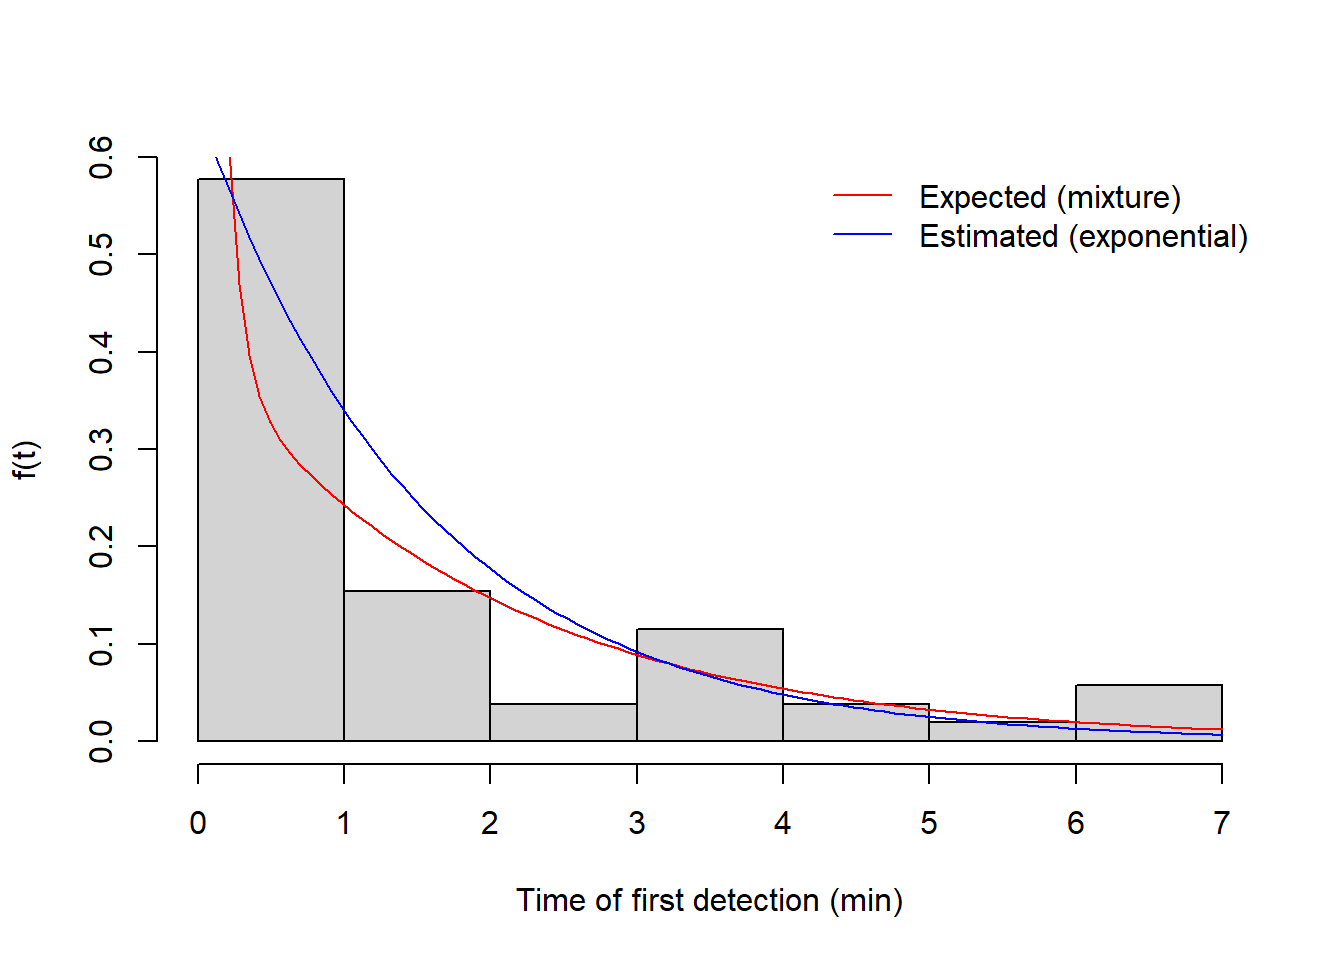
\includegraphics{qpad-book_files/figure-latex/unnamed-chunk-50-1.pdf}

\hypertarget{time-varying-conventional-removal-model}{%
\subsection{Time-varying conventional removal model}\label{time-varying-conventional-removal-model}}

Singing rates of birds vary with time of day, time of year, breeding status, and stage of the nesting cycle.
Thus, removal model estimates of availability may be improved by accounting for variation in singing rates
using covariates for day of year and time of day.
In this case \(p(t_{iJ}) = 1 - e^{-t_{iJ} \phi_{i}}\) and \(log(\phi_{i}) = \beta_{0} + \sum^{K}_{k=1} \beta_{k} x_{ik}\) is the linear predictor with \(K\) covariates and the corresponding unknown coefficients (\(\beta_{k}\), \(k = 0,\ldots, K\)).

Let's fit a couple of time-varying models using \texttt{DAY} and \texttt{TSSR} as covariates:

\begin{Shaded}
\begin{Highlighting}[]
\NormalTok{Me1 <-}\StringTok{ }\KeywordTok{cmulti}\NormalTok{(Y }\OperatorTok{|}\StringTok{ }\NormalTok{D }\OperatorTok{~}\StringTok{ }\NormalTok{DAY, X, }\DataTypeTok{type=}\StringTok{"rem"}\NormalTok{)}
\NormalTok{Me2 <-}\StringTok{ }\KeywordTok{cmulti}\NormalTok{(Y }\OperatorTok{|}\StringTok{ }\NormalTok{D }\OperatorTok{~}\StringTok{ }\NormalTok{TSSR, X, }\DataTypeTok{type=}\StringTok{"rem"}\NormalTok{)}
\end{Highlighting}
\end{Shaded}

Now compare the three conventional models based on AIC and inspect the summary for the best supported model with the \texttt{JDAY} effect.

\begin{Shaded}
\begin{Highlighting}[]
\NormalTok{Me_AIC <-}\StringTok{ }\KeywordTok{AIC}\NormalTok{(Me0, Me1, Me2)}
\NormalTok{Me_AIC}\OperatorTok{$}\NormalTok{delta_AIC <-}\StringTok{ }\NormalTok{Me_AIC}\OperatorTok{$}\NormalTok{AIC }\OperatorTok{-}\StringTok{ }\KeywordTok{min}\NormalTok{(Me_AIC}\OperatorTok{$}\NormalTok{AIC)}
\NormalTok{Me_AIC[}\KeywordTok{order}\NormalTok{(Me_AIC}\OperatorTok{$}\NormalTok{AIC),]}

\NormalTok{Me_Best <-}\StringTok{ }\KeywordTok{get}\NormalTok{(}\KeywordTok{rownames}\NormalTok{(Me_AIC)[Me_AIC}\OperatorTok{$}\NormalTok{delta_AIC }\OperatorTok{==}\StringTok{ }\DecValTok{0}\NormalTok{])}
\KeywordTok{summary}\NormalTok{(Me_Best)}
\end{Highlighting}
\end{Shaded}

\begin{verbatim}
## 
## Call:
## cmulti(formula = Y | D ~ DAY, data = X, type = "rem")
## 
## Removal Sampling (homogeneous singing rate)
## Conditional Maximum Likelihood estimates
## 
## Coefficients:
##                     Estimate Std. Error z value Pr(>|z|)    
## log.phi_(Intercept)   0.0784     0.2615    0.30  0.76427    
## log.phi_DAY          -2.0910     0.5866   -3.56  0.00036 ***
## ---
## Signif. codes:  0 '***' 0.001 '**' 0.01 '*' 0.05 '.' 0.1 ' ' 1 
## 
## Log-likelihood: -3.2e+03 
## BIC = 6.41e+03
\end{verbatim}

To visually capture the time-varying effects, we make some plots using base graphics,
colors matching the time-varying predictor. This way we can not only assess how availability
probability (given a fixed time interval) is changing with the values of the predictor,
but also how the cumulative distribution changes with time.

\begin{Shaded}
\begin{Highlighting}[]
\NormalTok{b <-}\StringTok{ }\KeywordTok{coef}\NormalTok{(Me_Best)}

\NormalTok{n <-}\StringTok{ }\DecValTok{100}
\NormalTok{DAY <-}\StringTok{ }\KeywordTok{seq}\NormalTok{(}\KeywordTok{min}\NormalTok{(X}\OperatorTok{$}\NormalTok{DAY), }\KeywordTok{max}\NormalTok{(X}\OperatorTok{$}\NormalTok{DAY), }\DataTypeTok{length.out=}\NormalTok{n}\OperatorTok{+}\DecValTok{1}\NormalTok{)}
\NormalTok{TSSR <-}\StringTok{ }\KeywordTok{seq}\NormalTok{(}\KeywordTok{min}\NormalTok{(X}\OperatorTok{$}\NormalTok{TSSR), }\KeywordTok{max}\NormalTok{(X}\OperatorTok{$}\NormalTok{TSSR), }\DataTypeTok{length.out=}\NormalTok{n}\OperatorTok{+}\DecValTok{1}\NormalTok{)}
\NormalTok{Duration <-}\StringTok{ }\KeywordTok{seq}\NormalTok{(}\DecValTok{0}\NormalTok{, }\DecValTok{10}\NormalTok{, }\DataTypeTok{length.out=}\NormalTok{n)}
\NormalTok{col <-}\StringTok{ }\KeywordTok{colorRampPalette}\NormalTok{(}\KeywordTok{c}\NormalTok{(}\StringTok{"red"}\NormalTok{, }\StringTok{"yellow"}\NormalTok{, }\StringTok{"blue"}\NormalTok{))(n)}

\NormalTok{op <-}\StringTok{ }\KeywordTok{par}\NormalTok{(}\DataTypeTok{mfrow=}\KeywordTok{c}\NormalTok{(}\DecValTok{1}\NormalTok{,}\DecValTok{2}\NormalTok{))}
\NormalTok{p1 <-}\StringTok{ }\DecValTok{1}\OperatorTok{-}\KeywordTok{exp}\NormalTok{(}\OperatorTok{-}\DecValTok{3}\OperatorTok{*}\KeywordTok{exp}\NormalTok{(b[}\DecValTok{1}\NormalTok{]}\OperatorTok{+}\NormalTok{b[}\DecValTok{2}\NormalTok{]}\OperatorTok{*}\NormalTok{DAY))}
\KeywordTok{plot}\NormalTok{(DAY, p1, }\DataTypeTok{ylim=}\KeywordTok{c}\NormalTok{(}\DecValTok{0}\NormalTok{,}\DecValTok{1}\NormalTok{), }\DataTypeTok{type=}\StringTok{"n"}\NormalTok{,}
    \DataTypeTok{main=}\KeywordTok{paste}\NormalTok{(spp, }\KeywordTok{rownames}\NormalTok{(Me_AIC)[Me_AIC}\OperatorTok{$}\NormalTok{delta_AIC }\OperatorTok{==}\StringTok{ }\DecValTok{0}\NormalTok{]),}
    \DataTypeTok{ylab=}\StringTok{"P(availability)"}\NormalTok{)}
\ControlFlowTok{for}\NormalTok{ (i }\ControlFlowTok{in} \KeywordTok{seq_len}\NormalTok{(n)) \{}
    \KeywordTok{lines}\NormalTok{(DAY[}\KeywordTok{c}\NormalTok{(i,i}\OperatorTok{+}\DecValTok{1}\NormalTok{)], p1[}\KeywordTok{c}\NormalTok{(i,i}\OperatorTok{+}\DecValTok{1}\NormalTok{)], }\DataTypeTok{col=}\NormalTok{col[i], }\DataTypeTok{lwd=}\DecValTok{2}\NormalTok{)}
\NormalTok{\}}
\KeywordTok{abline}\NormalTok{(}\DataTypeTok{h=}\KeywordTok{range}\NormalTok{(p1), }\DataTypeTok{col=}\StringTok{"grey"}\NormalTok{)}

\KeywordTok{plot}\NormalTok{(Duration, Duration, }\DataTypeTok{type=}\StringTok{"n"}\NormalTok{, }\DataTypeTok{ylim=}\KeywordTok{c}\NormalTok{(}\DecValTok{0}\NormalTok{,}\DecValTok{1}\NormalTok{),}
    \DataTypeTok{ylab=}\StringTok{"P(availability)"}\NormalTok{)}
\ControlFlowTok{for}\NormalTok{ (i }\ControlFlowTok{in} \KeywordTok{seq_len}\NormalTok{(n)) \{}
\NormalTok{    p2 <-}\StringTok{ }\DecValTok{1}\OperatorTok{-}\KeywordTok{exp}\NormalTok{(}\OperatorTok{-}\NormalTok{Duration}\OperatorTok{*}\KeywordTok{exp}\NormalTok{(b[}\DecValTok{1}\NormalTok{]}\OperatorTok{+}\NormalTok{b[}\DecValTok{2}\NormalTok{]}\OperatorTok{*}\NormalTok{DAY[i]))}
    \KeywordTok{lines}\NormalTok{(Duration, p2, }\DataTypeTok{col=}\NormalTok{col[i])}
\NormalTok{\}}
\KeywordTok{abline}\NormalTok{(}\DataTypeTok{v=}\DecValTok{3}\NormalTok{, }\DataTypeTok{h=}\KeywordTok{range}\NormalTok{(p1), }\DataTypeTok{col=}\StringTok{"grey"}\NormalTok{)}
\end{Highlighting}
\end{Shaded}

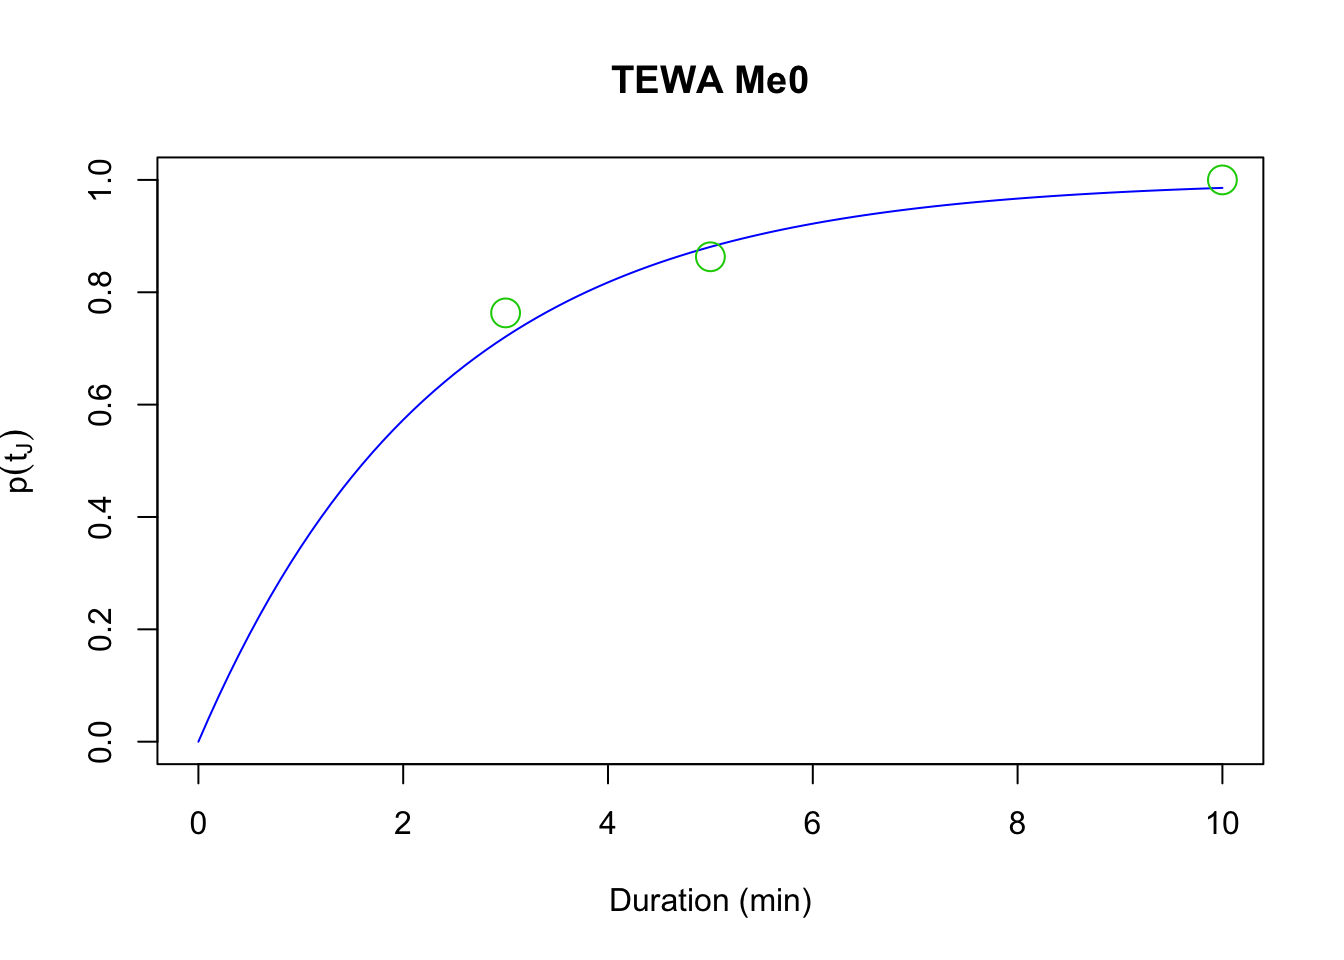
\includegraphics{qpad-book_files/figure-latex/unnamed-chunk-52-1.pdf}

\begin{Shaded}
\begin{Highlighting}[]
\KeywordTok{par}\NormalTok{(op)}
\end{Highlighting}
\end{Shaded}

\hypertarget{finite-mixtures}{%
\section{Finite mixtures}\label{finite-mixtures}}

Let's relax the assumption that all individuals vocalize at the same rate.
We can think about this as different groups in the population.
The individuals within the groups have homogenerous rates,
but the group level rates are different.
We can introduce such heterogeneity into our bSims world by
specifying the group level rates (\texttt{phi} vector) and the
proportion of individuals belonging to the groups (\texttt{mix}).

\begin{Shaded}
\begin{Highlighting}[]
\NormalTok{phi <-}\StringTok{ }\KeywordTok{c}\NormalTok{(}\DecValTok{10}\NormalTok{, }\FloatTok{0.5}\NormalTok{)}
\NormalTok{mix <-}\StringTok{ }\KeywordTok{c}\NormalTok{(}\FloatTok{0.25}\NormalTok{, }\FloatTok{0.75}\NormalTok{)}

\KeywordTok{set.seed}\NormalTok{(}\DecValTok{1}\NormalTok{)}
\NormalTok{(a2 <-}\StringTok{ }\KeywordTok{bsims_populate}\NormalTok{(l, }\DataTypeTok{density=}\DecValTok{1}\NormalTok{)) }\CommentTok{# increase density}
\end{Highlighting}
\end{Shaded}

\begin{verbatim}
## bSims population
##   1 km x 1 km
##   stratification: H
##   total abundance: 104
\end{verbatim}

\begin{Shaded}
\begin{Highlighting}[]
\NormalTok{(b2 <-}\StringTok{ }\KeywordTok{bsims_animate}\NormalTok{(a2, }\DataTypeTok{vocal_rate=}\NormalTok{phi, }\DataTypeTok{mixture=}\NormalTok{mix))}
\end{Highlighting}
\end{Shaded}

\begin{verbatim}
## bSims events
##   1 km x 1 km
##   stratification: H
##   total abundance: 104
##   mixture with total duration: 10
\end{verbatim}

\begin{Shaded}
\begin{Highlighting}[]
\NormalTok{b2}\OperatorTok{$}\NormalTok{vocal_rate}
\end{Highlighting}
\end{Shaded}

\begin{verbatim}
##   G1  G2
## H 10 0.5
## E 10 0.5
## R 10 0.5
\end{verbatim}

If we plot the time to first detection data, we can see how
expected distribution (red) is different from the fitted
Exponential distribution assuming homogeneity:

\begin{Shaded}
\begin{Highlighting}[]
\NormalTok{v <-}\StringTok{ }\KeywordTok{get_events}\NormalTok{(b2, }\DataTypeTok{vocal_only=}\OtherTok{TRUE}\NormalTok{)}
\NormalTok{v1 <-}\StringTok{ }\NormalTok{v[}\OperatorTok{!}\KeywordTok{duplicated}\NormalTok{(v}\OperatorTok{$}\NormalTok{i),]}
\NormalTok{(phi_hat <-}\StringTok{ }\KeywordTok{fitdistr}\NormalTok{(v1}\OperatorTok{$}\NormalTok{t, }\StringTok{"exponential"}\NormalTok{)}\OperatorTok{$}\NormalTok{estimate)}
\end{Highlighting}
\end{Shaded}

\begin{verbatim}
##   rate 
## 0.6522
\end{verbatim}

\begin{Shaded}
\begin{Highlighting}[]
\KeywordTok{hist}\NormalTok{(v1}\OperatorTok{$}\NormalTok{t, }\DataTypeTok{xlab=}\StringTok{"Time of first detection (min)"}\NormalTok{, }\DataTypeTok{freq=}\OtherTok{FALSE}\NormalTok{, }\DataTypeTok{main=}\StringTok{""}\NormalTok{, }
  \DataTypeTok{col=}\StringTok{"lightgrey"}\NormalTok{, }\DataTypeTok{ylab=}\StringTok{"f(t)"}\NormalTok{)}
\KeywordTok{curve}\NormalTok{(mix[}\DecValTok{1}\NormalTok{]}\OperatorTok{*}\KeywordTok{dexp}\NormalTok{(x, phi[}\DecValTok{1}\NormalTok{])}\OperatorTok{+}\NormalTok{mix[}\DecValTok{2}\NormalTok{]}\OperatorTok{*}\KeywordTok{dexp}\NormalTok{(x, phi[}\DecValTok{2}\NormalTok{]), }\DataTypeTok{add=}\OtherTok{TRUE}\NormalTok{, }\DataTypeTok{col=}\DecValTok{2}\NormalTok{)}
\KeywordTok{curve}\NormalTok{(}\KeywordTok{dexp}\NormalTok{(x, phi_hat), }\DataTypeTok{add=}\OtherTok{TRUE}\NormalTok{, }\DataTypeTok{col=}\DecValTok{4}\NormalTok{)}
\KeywordTok{legend}\NormalTok{(}\StringTok{"topright"}\NormalTok{, }\DataTypeTok{bty=}\StringTok{"n"}\NormalTok{, }\DataTypeTok{lty=}\DecValTok{1}\NormalTok{, }\DataTypeTok{col=}\KeywordTok{c}\NormalTok{(}\DecValTok{2}\NormalTok{,}\DecValTok{4}\NormalTok{), }
  \DataTypeTok{legend=}\KeywordTok{c}\NormalTok{(}\StringTok{"Expected (mixture)"}\NormalTok{, }\StringTok{"Estimated (exponential)"}\NormalTok{))}
\end{Highlighting}
\end{Shaded}

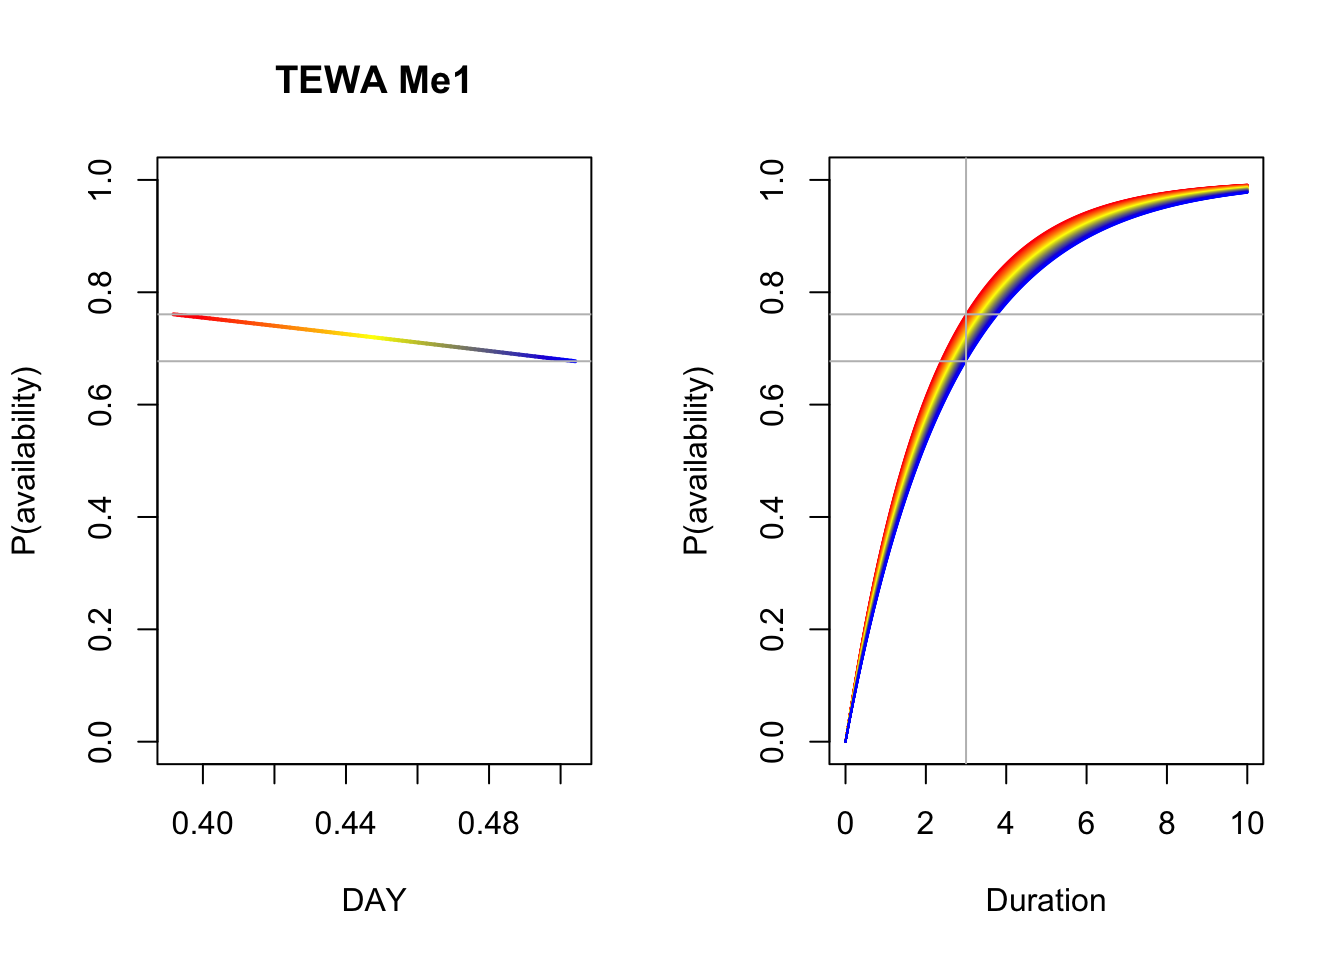
\includegraphics{qpad-book_files/figure-latex/unnamed-chunk-54-1.pdf}

Now let's visualize the corresponding cumulative distribution function:

\begin{Shaded}
\begin{Highlighting}[]
\NormalTok{br <-}\StringTok{ }\DecValTok{1}\OperatorTok{:}\DecValTok{10}
\NormalTok{i <-}\StringTok{ }\KeywordTok{cut}\NormalTok{(v1}\OperatorTok{$}\NormalTok{t, }\KeywordTok{c}\NormalTok{(}\DecValTok{0}\NormalTok{, br), }\DataTypeTok{include.lowest =} \OtherTok{TRUE}\NormalTok{)}
\KeywordTok{table}\NormalTok{(i)}
\end{Highlighting}
\end{Shaded}

\begin{verbatim}
## i
##  [0,1]  (1,2]  (2,3]  (3,4]  (4,5]  (5,6]  (6,7]  (7,8]  (8,9] (9,10] 
##     54     23     10      6      2      6      3      0      0      0
\end{verbatim}

\begin{Shaded}
\begin{Highlighting}[]
\KeywordTok{plot}\NormalTok{(}\KeywordTok{stepfun}\NormalTok{(v1}\OperatorTok{$}\NormalTok{t, (}\DecValTok{0}\OperatorTok{:}\KeywordTok{nrow}\NormalTok{(v1))}\OperatorTok{/}\KeywordTok{nrow}\NormalTok{(v1)), }\DataTypeTok{do.points=}\OtherTok{FALSE}\NormalTok{, }\DataTypeTok{xlim=}\KeywordTok{c}\NormalTok{(}\DecValTok{0}\NormalTok{,}\DecValTok{10}\NormalTok{),}
  \DataTypeTok{xlab=}\StringTok{"Time of first detection (min)"}\NormalTok{, }\DataTypeTok{ylab=}\StringTok{"F(t)"}\NormalTok{, }\DataTypeTok{main=}\StringTok{""}\NormalTok{)}
\KeywordTok{curve}\NormalTok{(}\DecValTok{1}\OperatorTok{-}\NormalTok{mix[}\DecValTok{2}\NormalTok{]}\OperatorTok{*}\KeywordTok{exp}\NormalTok{(}\OperatorTok{-}\NormalTok{phi[}\DecValTok{2}\NormalTok{]}\OperatorTok{*}\NormalTok{x), }\DataTypeTok{add=}\OtherTok{TRUE}\NormalTok{, }\DataTypeTok{col=}\DecValTok{2}\NormalTok{)}
\KeywordTok{curve}\NormalTok{(}\DecValTok{1}\OperatorTok{-}\KeywordTok{exp}\NormalTok{(}\OperatorTok{-}\NormalTok{phi_hat}\OperatorTok{*}\NormalTok{x), }\DataTypeTok{add=}\OtherTok{TRUE}\NormalTok{, }\DataTypeTok{col=}\DecValTok{4}\NormalTok{)}
\KeywordTok{legend}\NormalTok{(}\StringTok{"bottomright"}\NormalTok{, }\DataTypeTok{bty=}\StringTok{"n"}\NormalTok{, }\DataTypeTok{lty=}\KeywordTok{c}\NormalTok{(}\DecValTok{1}\NormalTok{,}\DecValTok{1}\NormalTok{,}\DecValTok{1}\NormalTok{,}\OtherTok{NA}\NormalTok{), }
  \DataTypeTok{col=}\KeywordTok{c}\NormalTok{(}\DecValTok{1}\NormalTok{,}\DecValTok{2}\NormalTok{,}\DecValTok{4}\NormalTok{,}\DecValTok{3}\NormalTok{), }\DataTypeTok{pch=}\KeywordTok{c}\NormalTok{(}\OtherTok{NA}\NormalTok{,}\OtherTok{NA}\NormalTok{,}\OtherTok{NA}\NormalTok{,}\DecValTok{21}\NormalTok{),}
  \DataTypeTok{legend=}\KeywordTok{c}\NormalTok{(}\StringTok{"Empirical"}\NormalTok{, }\StringTok{"Expected (mixture)"}\NormalTok{, }\StringTok{"Estimated (exponential)"}\NormalTok{, }\StringTok{"Binned"}\NormalTok{))}
\KeywordTok{points}\NormalTok{(br, }\KeywordTok{cumsum}\NormalTok{(}\KeywordTok{table}\NormalTok{(i))}\OperatorTok{/}\KeywordTok{sum}\NormalTok{(}\KeywordTok{table}\NormalTok{(i)), }\DataTypeTok{cex=}\DecValTok{2}\NormalTok{, }\DataTypeTok{col=}\DecValTok{3}\NormalTok{, }\DataTypeTok{pch=}\DecValTok{21}\NormalTok{)}
\end{Highlighting}
\end{Shaded}

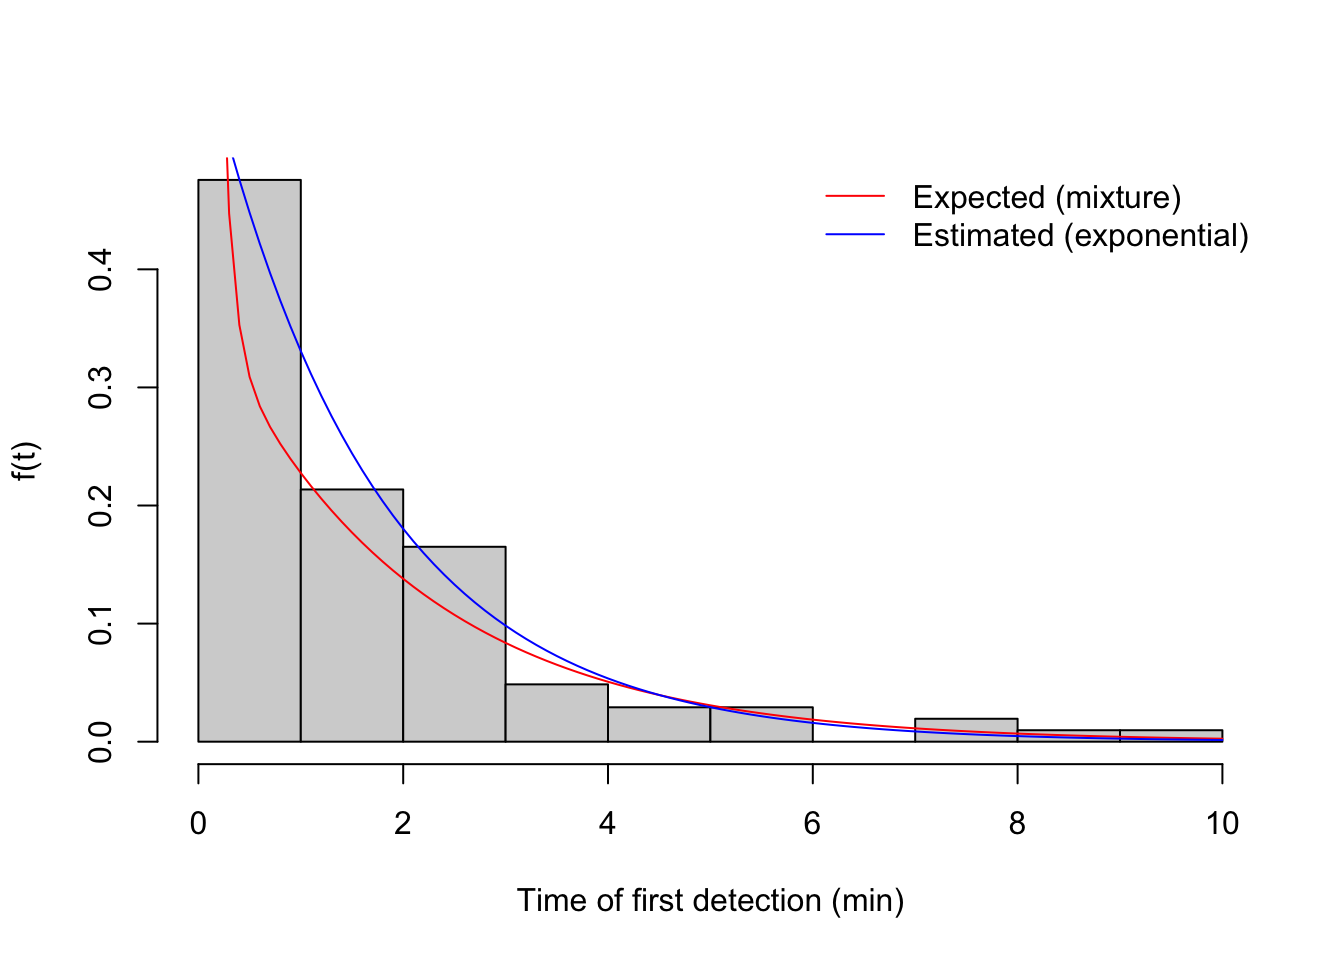
\includegraphics{qpad-book_files/figure-latex/unnamed-chunk-55-1.pdf}

We use the \texttt{detect::cmulti} function to fit the finite mixture model:

\begin{Shaded}
\begin{Highlighting}[]
\NormalTok{(y <-}\StringTok{ }\KeywordTok{matrix}\NormalTok{(}\KeywordTok{as.numeric}\NormalTok{(}\KeywordTok{table}\NormalTok{(i)), }\DataTypeTok{nrow=}\DecValTok{1}\NormalTok{))}
\end{Highlighting}
\end{Shaded}

\begin{verbatim}
##      [,1] [,2] [,3] [,4] [,5] [,6] [,7] [,8] [,9] [,10]
## [1,]   54   23   10    6    2    6    3    0    0     0
\end{verbatim}

\begin{Shaded}
\begin{Highlighting}[]
\NormalTok{(d <-}\StringTok{ }\KeywordTok{matrix}\NormalTok{(br, }\DataTypeTok{nrow=}\DecValTok{1}\NormalTok{))}
\end{Highlighting}
\end{Shaded}

\begin{verbatim}
##      [,1] [,2] [,3] [,4] [,5] [,6] [,7] [,8] [,9] [,10]
## [1,]    1    2    3    4    5    6    7    8    9    10
\end{verbatim}

\begin{Shaded}
\begin{Highlighting}[]
\NormalTok{cf <-}\StringTok{ }\KeywordTok{cmulti.fit}\NormalTok{(y, d, }\DataTypeTok{type=}\StringTok{"fmix"}\NormalTok{)}\OperatorTok{$}\NormalTok{coef }\CommentTok{# log.phi, logit.c}

\KeywordTok{c}\NormalTok{(}\DataTypeTok{phi=}\NormalTok{phi[}\DecValTok{2}\NormalTok{], }\DataTypeTok{c=}\NormalTok{mix[}\DecValTok{2}\NormalTok{]) }\CommentTok{# setting}
\end{Highlighting}
\end{Shaded}

\begin{verbatim}
##  phi    c 
## 0.50 0.75
\end{verbatim}

\begin{Shaded}
\begin{Highlighting}[]
\KeywordTok{c}\NormalTok{(}\DataTypeTok{phi_hat=}\KeywordTok{exp}\NormalTok{(cf[}\DecValTok{1}\NormalTok{]), }\DataTypeTok{c_hat=}\KeywordTok{plogis}\NormalTok{(cf[}\DecValTok{2}\NormalTok{])) }\CommentTok{# estimate}
\end{Highlighting}
\end{Shaded}

\begin{verbatim}
## phi_hat   c_hat 
##  0.5350  0.8244
\end{verbatim}

\hypertarget{time-invariant-finite-mixture-removal-model}{%
\subsection{Time-invariant finite mixture removal model}\label{time-invariant-finite-mixture-removal-model}}

The removal model can accommodate behavioral heterogeneity in singing by subdividing the
sampled population for a species at a given point into a finite mixture of birds with low and
high singing rates, which requires the additional estimation of the proportion of birds in the
sampled population with low singing rates.

In the continuous-time formulation of the finite mixture (or two-point mixture) removal model,
the cumulative density function during a point count is given by
\(p(t_{iJ}) = (1 - c) 1 + c (1 - e^{-t_{iJ} \phi}) = 1 - c e^{-t_{iJ} \phi}\), where
\(\phi\) is the singing rate for the group of infrequently singing birds, and \(c\) is the
proportion of birds during the point count that are infrequent singers. The remaining
proportions (\(1 - c\); the intercept of the cumulative density function) of the frequent
singers are assumed to be detected instantaneously at the start of the first time interval.
In the simplest form of the finite mixture model, the proportion and singing rate of birds
that sing infrequently is homogeneous across all times and locations (model \texttt{Mf0}).
We are using the \texttt{type\ =\ "fmix"} for finite mixture removal models.

Here, for the read bird data set:

\begin{Shaded}
\begin{Highlighting}[]
\NormalTok{Mf0 <-}\StringTok{ }\KeywordTok{cmulti}\NormalTok{(Y }\OperatorTok{|}\StringTok{ }\NormalTok{D }\OperatorTok{~}\StringTok{ }\DecValTok{1}\NormalTok{, }\DataTypeTok{type=}\StringTok{"fmix"}\NormalTok{)}
\KeywordTok{summary}\NormalTok{(Mf0)}
\end{Highlighting}
\end{Shaded}

\begin{verbatim}
## 
## Call:
## cmulti(formula = Y | D ~ 1, type = "fmix")
## 
## Removal Sampling (heterogeneous singing rate)
## Conditional Maximum Likelihood estimates
## 
## Coefficients:
##                     Estimate Std. Error z value Pr(>|z|)    
## log.phi_(Intercept)  -1.7146     0.0970  -17.68   <2e-16 ***
## logit.c               0.0742     0.0598    1.24     0.21    
## ---
## Signif. codes:  0 '***' 0.001 '**' 0.01 '*' 0.05 '.' 0.1 ' ' 1 
## 
## Log-likelihood: -3.1e+03 
## BIC = 6.22e+03
\end{verbatim}

\begin{Shaded}
\begin{Highlighting}[]
\NormalTok{cf_Mf0 <-}\StringTok{ }\KeywordTok{coef}\NormalTok{(Mf0)}

\KeywordTok{curve}\NormalTok{(}\DecValTok{1}\OperatorTok{-}\KeywordTok{plogis}\NormalTok{(cf_Mf0[}\DecValTok{2}\NormalTok{]) }\OperatorTok{*}\StringTok{ }\KeywordTok{exp}\NormalTok{(}\OperatorTok{-}\NormalTok{x}\OperatorTok{*}\KeywordTok{exp}\NormalTok{(cf_Mf0[}\DecValTok{1}\NormalTok{])), }
  \DataTypeTok{xlim=}\KeywordTok{c}\NormalTok{(}\DecValTok{0}\NormalTok{, }\DecValTok{10}\NormalTok{), }\DataTypeTok{ylim=}\KeywordTok{c}\NormalTok{(}\DecValTok{0}\NormalTok{, }\DecValTok{1}\NormalTok{), }\DataTypeTok{col=}\DecValTok{4}\NormalTok{, }\DataTypeTok{main=}\KeywordTok{paste}\NormalTok{(spp, }\StringTok{"Mf0"}\NormalTok{),}
  \DataTypeTok{xlab=}\StringTok{"Duration (min)"}\NormalTok{, }\DataTypeTok{ylab=}\KeywordTok{expression}\NormalTok{(}\KeywordTok{p}\NormalTok{(t[J])))}
\KeywordTok{points}\NormalTok{(D[}\DecValTok{1}\NormalTok{,], }\KeywordTok{cumsum}\NormalTok{(}\KeywordTok{colSums}\NormalTok{(Y))}\OperatorTok{/}\KeywordTok{sum}\NormalTok{(Y), }\DataTypeTok{cex=}\DecValTok{2}\NormalTok{, }\DataTypeTok{col=}\DecValTok{3}\NormalTok{, }\DataTypeTok{pch=}\DecValTok{21}\NormalTok{)}
\end{Highlighting}
\end{Shaded}

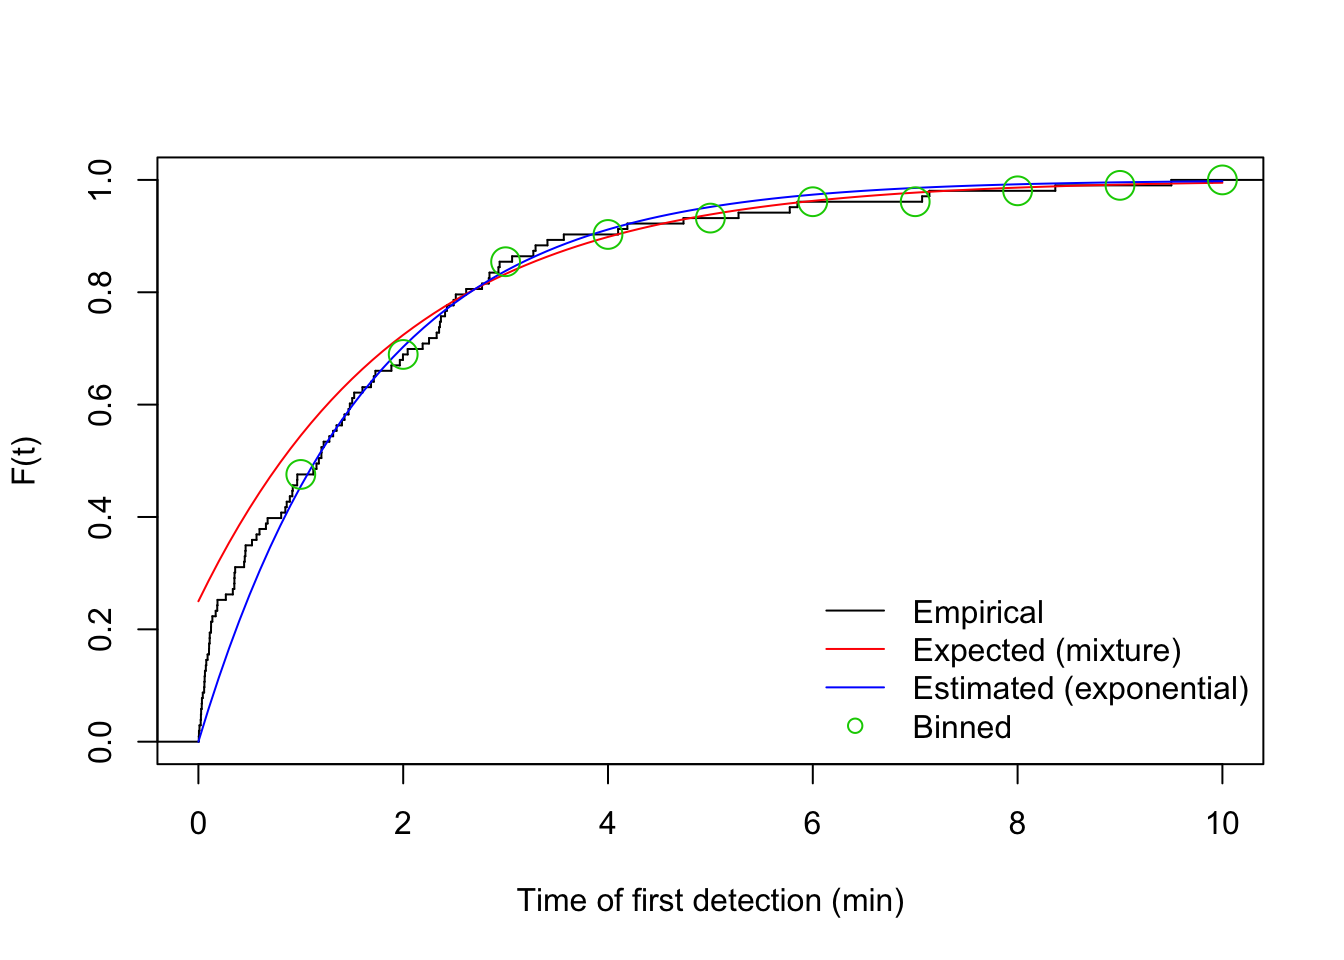
\includegraphics{qpad-book_files/figure-latex/unnamed-chunk-57-1.pdf}

\hypertarget{time-varying-finite-mixture-removal-models}{%
\subsection{Time-varying finite mixture removal models}\label{time-varying-finite-mixture-removal-models}}

Previously, researchers have applied covariate effects on the parameter
\(\phi_{i}\) of the finite mixture model, similarly to how we modeled these effects in conventional models.
This model assumes that the parameter \(c\) is constant irrespective of time and location
(i.e.~only the infrequent singer group changes its singing behavior).

We can fit finite mixture models with \texttt{DAY} and \texttt{TSSR} as covariates on \(\phi\).
In this case \(p(t_{iJ}) = 1 - c e^{-t_{iJ} \phi_{i}}\) and
\(log(\phi_{i}) = \beta_{0} + \sum^{K}_{k=1} \beta_{k} x_{ik}\)
is the linear predictor with \(K\) covariates and the corresponding unknown coefficients
(\(\beta_{k}\), \(k = 0,\ldots, K\)).

\begin{Shaded}
\begin{Highlighting}[]
\NormalTok{Mf1 <-}\StringTok{ }\KeywordTok{cmulti}\NormalTok{(Y }\OperatorTok{|}\StringTok{ }\NormalTok{D }\OperatorTok{~}\StringTok{ }\NormalTok{DAY, X, }\DataTypeTok{type=}\StringTok{"fmix"}\NormalTok{)}
\NormalTok{Mf2 <-}\StringTok{ }\KeywordTok{cmulti}\NormalTok{(Y }\OperatorTok{|}\StringTok{ }\NormalTok{D }\OperatorTok{~}\StringTok{ }\NormalTok{TSSR, X, }\DataTypeTok{type=}\StringTok{"fmix"}\NormalTok{)}
\end{Highlighting}
\end{Shaded}

Compare the three finite mixture models based on AIC and inspect the summary for the best supported
model:

\begin{Shaded}
\begin{Highlighting}[]
\NormalTok{Mf_AIC <-}\StringTok{ }\KeywordTok{AIC}\NormalTok{(Mf0, Mf1, Mf2)}
\NormalTok{Mf_AIC}\OperatorTok{$}\NormalTok{delta_AIC <-}\StringTok{ }\NormalTok{Mf_AIC}\OperatorTok{$}\NormalTok{AIC }\OperatorTok{-}\StringTok{ }\KeywordTok{min}\NormalTok{(Mf_AIC}\OperatorTok{$}\NormalTok{AIC)}

\NormalTok{Mf_Best <-}\StringTok{ }\KeywordTok{get}\NormalTok{(}\KeywordTok{rownames}\NormalTok{(Mf_AIC)[Mf_AIC}\OperatorTok{$}\NormalTok{delta_AIC }\OperatorTok{==}\StringTok{ }\DecValTok{0}\NormalTok{])}
\NormalTok{Mf_AIC[}\KeywordTok{order}\NormalTok{(Mf_AIC}\OperatorTok{$}\NormalTok{AIC),]}

\KeywordTok{summary}\NormalTok{(Mf_Best)}
\end{Highlighting}
\end{Shaded}

\begin{verbatim}
## 
## Call:
## cmulti(formula = Y | D ~ DAY, data = X, type = "fmix")
## 
## Removal Sampling (heterogeneous singing rate)
## Conditional Maximum Likelihood estimates
## 
## Coefficients:
##                     Estimate Std. Error z value Pr(>|z|)   
## log.phi_(Intercept)    0.754      0.848    0.89   0.3739   
## log.phi_DAY           -5.412      1.938   -2.79   0.0052 **
## logit.c                0.119      0.062    1.92   0.0548 . 
## ---
## Signif. codes:  0 '***' 0.001 '**' 0.01 '*' 0.05 '.' 0.1 ' ' 1 
## 
## Log-likelihood: -3.1e+03 
## BIC = 6.22e+03
\end{verbatim}

We produce a similar plot as before.

\begin{Shaded}
\begin{Highlighting}[]
\NormalTok{b <-}\StringTok{ }\KeywordTok{coef}\NormalTok{(Mf_Best)}

\NormalTok{op <-}\StringTok{ }\KeywordTok{par}\NormalTok{(}\DataTypeTok{mfrow=}\KeywordTok{c}\NormalTok{(}\DecValTok{1}\NormalTok{,}\DecValTok{2}\NormalTok{))}
\NormalTok{p1 <-}\StringTok{ }\DecValTok{1}\OperatorTok{-}\KeywordTok{plogis}\NormalTok{(b[}\DecValTok{3}\NormalTok{])}\OperatorTok{*}\KeywordTok{exp}\NormalTok{(}\OperatorTok{-}\DecValTok{3}\OperatorTok{*}\KeywordTok{exp}\NormalTok{(b[}\DecValTok{1}\NormalTok{]}\OperatorTok{+}\NormalTok{b[}\DecValTok{2}\NormalTok{]}\OperatorTok{*}\NormalTok{DAY))}
\KeywordTok{plot}\NormalTok{(DAY, p1, }\DataTypeTok{ylim=}\KeywordTok{c}\NormalTok{(}\DecValTok{0}\NormalTok{,}\DecValTok{1}\NormalTok{), }\DataTypeTok{type=}\StringTok{"n"}\NormalTok{,}
    \DataTypeTok{main=}\KeywordTok{paste}\NormalTok{(spp, }\KeywordTok{rownames}\NormalTok{(Mf_AIC)[Mf_AIC}\OperatorTok{$}\NormalTok{delta_AIC }\OperatorTok{==}\StringTok{ }\DecValTok{0}\NormalTok{]),}
    \DataTypeTok{ylab=}\StringTok{"P(availability)"}\NormalTok{)}
\ControlFlowTok{for}\NormalTok{ (i }\ControlFlowTok{in} \KeywordTok{seq_len}\NormalTok{(n)) \{}
    \KeywordTok{lines}\NormalTok{(DAY[}\KeywordTok{c}\NormalTok{(i,i}\OperatorTok{+}\DecValTok{1}\NormalTok{)], p1[}\KeywordTok{c}\NormalTok{(i,i}\OperatorTok{+}\DecValTok{1}\NormalTok{)], }\DataTypeTok{col=}\NormalTok{col[i], }\DataTypeTok{lwd=}\DecValTok{2}\NormalTok{)}
\NormalTok{\}}
\KeywordTok{abline}\NormalTok{(}\DataTypeTok{h=}\KeywordTok{range}\NormalTok{(p1), }\DataTypeTok{col=}\StringTok{"grey"}\NormalTok{)}

\KeywordTok{plot}\NormalTok{(Duration, Duration, }\DataTypeTok{type=}\StringTok{"n"}\NormalTok{, }\DataTypeTok{ylim=}\KeywordTok{c}\NormalTok{(}\DecValTok{0}\NormalTok{,}\DecValTok{1}\NormalTok{),}
    \DataTypeTok{ylab=}\StringTok{"P(availability)"}\NormalTok{)}
\ControlFlowTok{for}\NormalTok{ (i }\ControlFlowTok{in} \KeywordTok{seq_len}\NormalTok{(n)) \{}
\NormalTok{    p2 <-}\StringTok{ }\DecValTok{1}\OperatorTok{-}\KeywordTok{plogis}\NormalTok{(b[}\DecValTok{3}\NormalTok{])}\OperatorTok{*}\KeywordTok{exp}\NormalTok{(}\OperatorTok{-}\NormalTok{Duration}\OperatorTok{*}\KeywordTok{exp}\NormalTok{(b[}\DecValTok{1}\NormalTok{]}\OperatorTok{+}\NormalTok{b[}\DecValTok{2}\NormalTok{]}\OperatorTok{*}\NormalTok{DAY[i]))}
    \KeywordTok{lines}\NormalTok{(Duration, p2, }\DataTypeTok{col=}\NormalTok{col[i])}
\NormalTok{\}}
\KeywordTok{abline}\NormalTok{(}\DataTypeTok{v=}\DecValTok{3}\NormalTok{, }\DataTypeTok{h=}\KeywordTok{range}\NormalTok{(p1), }\DataTypeTok{col=}\StringTok{"grey"}\NormalTok{)}
\end{Highlighting}
\end{Shaded}

\includegraphics{qpad-book_files/figure-latex/unnamed-chunk-60-1.pdf}

\begin{Shaded}
\begin{Highlighting}[]
\KeywordTok{par}\NormalTok{(op)}
\end{Highlighting}
\end{Shaded}

An alternative parametrization is that \(c_{i}\) rather than \(\phi\) be the time-varying parameter,
allowing the individuals to switch between the frequent and infrequent group depending on covariates.
We can fit this class of finite mixture model with \texttt{DAY} and \texttt{TSSR} as covariates on \(c\)
using \texttt{type\ =\ "mix"} (instead of \texttt{"fmix"}).
In this case \(p(t_{iJ}) = 1 - c_{i} e^{-t_{iJ} \phi}\) and
\(logit(c_{i}) = \beta_{0} + \sum^{K}_{k=1} \beta_{k} x_{ik}\) is the linear predictor with \(K\)
covariates and the corresponding unknown coefficients (\(\beta_{k}\), \(k = 0,\ldots, K\)).
Because \(c_{i}\) is a proportion, we model it on the logit scale.

\begin{Shaded}
\begin{Highlighting}[]
\NormalTok{Mm1 <-}\StringTok{ }\KeywordTok{cmulti}\NormalTok{(Y }\OperatorTok{|}\StringTok{ }\NormalTok{D }\OperatorTok{~}\StringTok{ }\NormalTok{DAY, X, }\DataTypeTok{type=}\StringTok{"mix"}\NormalTok{)}
\NormalTok{Mm2 <-}\StringTok{ }\KeywordTok{cmulti}\NormalTok{(Y }\OperatorTok{|}\StringTok{ }\NormalTok{D }\OperatorTok{~}\StringTok{ }\NormalTok{TSSR, X, }\DataTypeTok{type=}\StringTok{"mix"}\NormalTok{)}
\end{Highlighting}
\end{Shaded}

We did not fit a null model for this parametrization, because it is identical to the \texttt{Mf0} model,
so that model \texttt{Mf0} is what we use to compare AIC values and inspect the summary for the best
supported model:

\begin{Shaded}
\begin{Highlighting}[]
\NormalTok{Mm_AIC <-}\StringTok{ }\KeywordTok{AIC}\NormalTok{(Mf0, Mm1, Mm2)}
\NormalTok{Mm_AIC}\OperatorTok{$}\NormalTok{delta_AIC <-}\StringTok{ }\NormalTok{Mm_AIC}\OperatorTok{$}\NormalTok{AIC }\OperatorTok{-}\StringTok{ }\KeywordTok{min}\NormalTok{(Mm_AIC}\OperatorTok{$}\NormalTok{AIC)}

\NormalTok{Mm_Best <-}\StringTok{ }\KeywordTok{get}\NormalTok{(}\KeywordTok{rownames}\NormalTok{(Mm_AIC)[Mm_AIC}\OperatorTok{$}\NormalTok{delta_AIC }\OperatorTok{==}\StringTok{ }\DecValTok{0}\NormalTok{])}
\NormalTok{Mm_AIC[}\KeywordTok{order}\NormalTok{(Mm_AIC}\OperatorTok{$}\NormalTok{AIC),]}

\KeywordTok{summary}\NormalTok{(Mm_Best)}
\end{Highlighting}
\end{Shaded}

\begin{verbatim}
## 
## Call:
## cmulti(formula = Y | D ~ DAY, data = X, type = "mix")
## 
## Removal Sampling (heterogeneous singing rate)
## Conditional Maximum Likelihood estimates
## 
## Coefficients:
##                     Estimate Std. Error z value Pr(>|z|)    
## log.phi               -1.716      0.097  -17.69   <2e-16 ***
## logit.c_(Intercept)   -2.070      0.692   -2.99   0.0028 ** 
## logit.c_DAY            4.804      1.558    3.08   0.0020 ** 
## ---
## Signif. codes:  0 '***' 0.001 '**' 0.01 '*' 0.05 '.' 0.1 ' ' 1 
## 
## Log-likelihood: -3.1e+03 
## BIC = 6.22e+03
\end{verbatim}

We produce a similar plot as before:

\begin{Shaded}
\begin{Highlighting}[]
\NormalTok{b <-}\StringTok{ }\KeywordTok{coef}\NormalTok{(Mm_Best)}

\NormalTok{op <-}\StringTok{ }\KeywordTok{par}\NormalTok{(}\DataTypeTok{mfrow=}\KeywordTok{c}\NormalTok{(}\DecValTok{1}\NormalTok{,}\DecValTok{2}\NormalTok{))}
\NormalTok{p1 <-}\StringTok{ }\DecValTok{1}\OperatorTok{-}\KeywordTok{plogis}\NormalTok{(b[}\DecValTok{2}\NormalTok{]}\OperatorTok{+}\NormalTok{b[}\DecValTok{3}\NormalTok{]}\OperatorTok{*}\NormalTok{DAY)}\OperatorTok{*}\KeywordTok{exp}\NormalTok{(}\OperatorTok{-}\DecValTok{3}\OperatorTok{*}\KeywordTok{exp}\NormalTok{(b[}\DecValTok{1}\NormalTok{]))}
\KeywordTok{plot}\NormalTok{(DAY, p1, }\DataTypeTok{ylim=}\KeywordTok{c}\NormalTok{(}\DecValTok{0}\NormalTok{,}\DecValTok{1}\NormalTok{), }\DataTypeTok{type=}\StringTok{"n"}\NormalTok{,}
    \DataTypeTok{main=}\KeywordTok{paste}\NormalTok{(spp, }\KeywordTok{rownames}\NormalTok{(Mm_AIC)[Mm_AIC}\OperatorTok{$}\NormalTok{delta_AIC }\OperatorTok{==}\StringTok{ }\DecValTok{0}\NormalTok{]),}
    \DataTypeTok{ylab=}\StringTok{"P(availability)"}\NormalTok{)}
\ControlFlowTok{for}\NormalTok{ (i }\ControlFlowTok{in} \KeywordTok{seq_len}\NormalTok{(n)) \{}
    \KeywordTok{lines}\NormalTok{(DAY[}\KeywordTok{c}\NormalTok{(i,i}\OperatorTok{+}\DecValTok{1}\NormalTok{)], p1[}\KeywordTok{c}\NormalTok{(i,i}\OperatorTok{+}\DecValTok{1}\NormalTok{)], }\DataTypeTok{col=}\NormalTok{col[i], }\DataTypeTok{lwd=}\DecValTok{2}\NormalTok{)}
\NormalTok{\}}
\KeywordTok{abline}\NormalTok{(}\DataTypeTok{h=}\KeywordTok{range}\NormalTok{(p1), }\DataTypeTok{col=}\StringTok{"grey"}\NormalTok{)}

\KeywordTok{plot}\NormalTok{(Duration, Duration, }\DataTypeTok{type=}\StringTok{"n"}\NormalTok{, }\DataTypeTok{ylim=}\KeywordTok{c}\NormalTok{(}\DecValTok{0}\NormalTok{,}\DecValTok{1}\NormalTok{),}
    \DataTypeTok{ylab=}\StringTok{"P(availability)"}\NormalTok{)}
\ControlFlowTok{for}\NormalTok{ (i }\ControlFlowTok{in} \KeywordTok{seq_len}\NormalTok{(n)) \{}
\NormalTok{    p2 <-}\StringTok{ }\DecValTok{1}\OperatorTok{-}\KeywordTok{plogis}\NormalTok{(b[}\DecValTok{2}\NormalTok{]}\OperatorTok{+}\NormalTok{b[}\DecValTok{3}\NormalTok{]}\OperatorTok{*}\NormalTok{DAY[i])}\OperatorTok{*}\KeywordTok{exp}\NormalTok{(}\OperatorTok{-}\NormalTok{Duration}\OperatorTok{*}\KeywordTok{exp}\NormalTok{(b[}\DecValTok{1}\NormalTok{]))}
    \KeywordTok{lines}\NormalTok{(Duration, p2, }\DataTypeTok{col=}\NormalTok{col[i])}
\NormalTok{\}}
\KeywordTok{abline}\NormalTok{(}\DataTypeTok{v=}\DecValTok{3}\NormalTok{, }\DataTypeTok{h=}\KeywordTok{range}\NormalTok{(p1), }\DataTypeTok{col=}\StringTok{"grey"}\NormalTok{)}
\end{Highlighting}
\end{Shaded}

\includegraphics{qpad-book_files/figure-latex/unnamed-chunk-63-1.pdf}

\begin{Shaded}
\begin{Highlighting}[]
\KeywordTok{par}\NormalTok{(op)}
\end{Highlighting}
\end{Shaded}

\hypertarget{let-the-best-model-win}{%
\section{Let the best model win}\label{let-the-best-model-win}}

So which of the 3 parametrizations proved to be best for our data?
It was the finite mixture with time-varying proportion of infrequent singers.
Second was the other finite mixture model, while the conventional model
was lagging behind.

\begin{Shaded}
\begin{Highlighting}[]
\NormalTok{M_AIC <-}\StringTok{ }\KeywordTok{AIC}\NormalTok{(Me_Best, Mf_Best, Mm_Best)}
\NormalTok{M_AIC}\OperatorTok{$}\NormalTok{delta_AIC <-}\StringTok{ }\NormalTok{M_AIC}\OperatorTok{$}\NormalTok{AIC }\OperatorTok{-}\StringTok{ }\KeywordTok{min}\NormalTok{(M_AIC}\OperatorTok{$}\NormalTok{AIC)}
\NormalTok{M_AIC[}\KeywordTok{order}\NormalTok{(M_AIC}\OperatorTok{$}\NormalTok{AIC),]}
\end{Highlighting}
\end{Shaded}

Finite mixture models provide some really nice insight into how singing behavior changes over time and, due to more parameters, they provide a better fit and thus minimize bias in population size estimates. But all this improvement comes with a price: sample size requirements (or more precisely, the number of detections required) are really high. To have all the benefits with reduced variance, one needs about 1000 non-zero observations to fit finite mixture models, 20 times more than needed to reliably fit conventional removal models. This is much higher than previously suggested minimum sample sizes.

Our findings also indicate that lengthening the count duration from 3 minutes to 5--10 minutes is an important consideration when designing field surveys to increase the accuracy and precision of population estimates. Well-informed survey design combined with various forms of removal sampling are useful in accounting for availability bias in point counts, thereby improving population estimates, and allowing for better integration of disparate studies at larger spatial scales.

\BeginKnitrBlock{rmdexercise}
\textbf{Exercise}

Compare different durations, numbers and lengths of time intervals when estimating vocalization rates.

Estimate vocalization rates for other species (e.g.~rare species, specias with less frequent vocalizations).

Compare linear and polynomial \texttt{DAY} effects for migratory and resident species (e.g.~BCCH, BOCH, BRCR, CORA, GRAJ, RBNU).
\EndKnitrBlock{rmdexercise}

\hypertarget{estimating-abundance}{%
\section{Estimating abundance}\label{estimating-abundance}}

Let us use the bSims approach to see how well we can estimate abundance
after accounting for availability. We set \texttt{Den} as density (\(D\)), and because
area is \(A\) = 100 ha by default, the expected value of the abundance (\(\lambda\))
bacomes \(AD\), while the actual abundance (\(N\)) is a realization of that
based on Poisson distribution (\(N \sim Poisson(\lambda)\)):

\begin{Shaded}
\begin{Highlighting}[]
\NormalTok{phi <-}\StringTok{ }\FloatTok{0.5}
\NormalTok{Den <-}\StringTok{ }\DecValTok{1}

\KeywordTok{set.seed}\NormalTok{(}\DecValTok{1}\NormalTok{)}
\NormalTok{l <-}\StringTok{ }\KeywordTok{bsims_init}\NormalTok{()}
\NormalTok{a <-}\StringTok{ }\KeywordTok{bsims_populate}\NormalTok{(l, }\DataTypeTok{density=}\NormalTok{Den)}
\NormalTok{(b <-}\StringTok{ }\KeywordTok{bsims_animate}\NormalTok{(a, }\DataTypeTok{vocal_rate=}\NormalTok{phi, }\DataTypeTok{move_rate=}\DecValTok{0}\NormalTok{))}
\end{Highlighting}
\end{Shaded}

\begin{verbatim}
## bSims events
##   1 km x 1 km
##   stratification: H
##   total abundance: 104
##   total duration: 10
\end{verbatim}

The next function we use is \texttt{bsims\_transcribe} which takes the events data
and bins it according to time intervals, \texttt{tint} defines the end times of
each interval:

\begin{Shaded}
\begin{Highlighting}[]
\NormalTok{tint <-}\StringTok{ }\KeywordTok{c}\NormalTok{(}\DecValTok{1}\NormalTok{, }\DecValTok{2}\NormalTok{, }\DecValTok{3}\NormalTok{, }\DecValTok{4}\NormalTok{, }\DecValTok{5}\NormalTok{)}
\NormalTok{(tr <-}\StringTok{ }\KeywordTok{bsims_transcribe}\NormalTok{(b, }\DataTypeTok{tint=}\NormalTok{tint))}
\end{Highlighting}
\end{Shaded}

\begin{verbatim}
## bSims transcript
##   1 km x 1 km
##   stratification: H
##   total abundance: 104
##   total duration: 10
##   detected: 104 heard
##   1st inds. [0-1, 1-2, 2-3, 3-4, 4-5 min] [0+ m]
\end{verbatim}

\begin{Shaded}
\begin{Highlighting}[]
\NormalTok{tr}\OperatorTok{$}\NormalTok{removal }\CommentTok{# binned new individuals}
\end{Highlighting}
\end{Shaded}

\begin{verbatim}
##     0-1min 1-2min 2-3min 3-4min 4-5min
## 0+m     35     28     16     12      6
\end{verbatim}

\begin{Shaded}
\begin{Highlighting}[]
\NormalTok{(Y <-}\StringTok{ }\KeywordTok{sum}\NormalTok{(tr}\OperatorTok{$}\NormalTok{removal)) }\CommentTok{# detected in 0-3 min}
\end{Highlighting}
\end{Shaded}

\begin{verbatim}
## [1] 97
\end{verbatim}

After \texttt{max(tint)} duration, we detected \(Y\) individuals.
Because \(E[Y] = NC\), we only have to estimate the correction factor \(C\),
that happens to be \(C=p\) in this case because our bSims world
ignored the observation process so far. \(p\) is estimated based on \(\phi\):

\begin{Shaded}
\begin{Highlighting}[]
\NormalTok{fit <-}\StringTok{ }\KeywordTok{cmulti.fit}\NormalTok{(tr}\OperatorTok{$}\NormalTok{removal, }\KeywordTok{matrix}\NormalTok{(tint, }\DataTypeTok{nrow=}\DecValTok{1}\NormalTok{), }\DataTypeTok{type=}\StringTok{"rem"}\NormalTok{)}
\KeywordTok{c}\NormalTok{(}\DataTypeTok{true=}\NormalTok{phi, }\DataTypeTok{estimate=}\KeywordTok{exp}\NormalTok{(fit}\OperatorTok{$}\NormalTok{coef))}
\end{Highlighting}
\end{Shaded}

\begin{verbatim}
##     true estimate 
##   0.5000   0.4083
\end{verbatim}

\begin{Shaded}
\begin{Highlighting}[]
\NormalTok{(p <-}\StringTok{ }\DecValTok{1}\OperatorTok{-}\KeywordTok{exp}\NormalTok{(}\OperatorTok{-}\KeywordTok{max}\NormalTok{(tint)}\OperatorTok{*}\KeywordTok{exp}\NormalTok{(fit}\OperatorTok{$}\NormalTok{coef)))}
\end{Highlighting}
\end{Shaded}

\begin{verbatim}
## [1] 0.8702
\end{verbatim}

Our estimate of \(N\) becomes \(Y/C=Y/p\):

\begin{Shaded}
\begin{Highlighting}[]
\NormalTok{N <-}\StringTok{ }\KeywordTok{sum}\NormalTok{(a}\OperatorTok{$}\NormalTok{abundance)}
\NormalTok{Nhat <-}\StringTok{ }\NormalTok{Y}\OperatorTok{/}\NormalTok{p}
\KeywordTok{c}\NormalTok{(}\DataTypeTok{true=}\NormalTok{N, }\DataTypeTok{estimate=}\NormalTok{Nhat)}
\end{Highlighting}
\end{Shaded}

\begin{verbatim}
##     true estimate 
##    104.0    111.5
\end{verbatim}

In this case, area is known, so density becomes:

\begin{Shaded}
\begin{Highlighting}[]
\NormalTok{A <-}\StringTok{ }\KeywordTok{sum}\NormalTok{(a}\OperatorTok{$}\NormalTok{area)}
\KeywordTok{c}\NormalTok{(}\DataTypeTok{true=}\NormalTok{N }\OperatorTok{/}\StringTok{ }\NormalTok{A, }\DataTypeTok{estimate=}\NormalTok{Nhat }\OperatorTok{/}\StringTok{ }\NormalTok{A)}
\end{Highlighting}
\end{Shaded}

\begin{verbatim}
##     true estimate 
##    1.040    1.115
\end{verbatim}

Next we use the \texttt{Best} model from our real JOSM bird data analysis:

\begin{Shaded}
\begin{Highlighting}[]
\NormalTok{spp <-}\StringTok{ "TEWA"}

\NormalTok{Y <-}\StringTok{ }\KeywordTok{as.matrix}\NormalTok{(yall[[spp]])}
\NormalTok{D <-}\StringTok{ }\KeywordTok{matrix}\NormalTok{(}\KeywordTok{c}\NormalTok{(}\DecValTok{3}\NormalTok{, }\DecValTok{5}\NormalTok{, }\DecValTok{10}\NormalTok{), }\KeywordTok{nrow}\NormalTok{(Y), }\DecValTok{3}\NormalTok{, }\DataTypeTok{byrow=}\OtherTok{TRUE}\NormalTok{,}
  \DataTypeTok{dimnames=}\KeywordTok{dimnames}\NormalTok{(Y))}
\NormalTok{X <-}\StringTok{ }\NormalTok{josm}\OperatorTok{$}\NormalTok{surveys[}\KeywordTok{rownames}\NormalTok{(Y), }\KeywordTok{c}\NormalTok{(}\StringTok{"DAY"}\NormalTok{, }\StringTok{"TSSR"}\NormalTok{)]}

\NormalTok{Best <-}\StringTok{ }\KeywordTok{get}\NormalTok{(}\KeywordTok{rownames}\NormalTok{(M_AIC)[M_AIC}\OperatorTok{$}\NormalTok{delta_AIC }\OperatorTok{==}\StringTok{ }\DecValTok{0}\NormalTok{])}
\KeywordTok{summary}\NormalTok{(Best)}
\end{Highlighting}
\end{Shaded}

\begin{verbatim}
## 
## Call:
## cmulti(formula = Y | D ~ DAY, data = X, type = "mix")
## 
## Removal Sampling (heterogeneous singing rate)
## Conditional Maximum Likelihood estimates
## 
## Coefficients:
##                     Estimate Std. Error z value Pr(>|z|)    
## log.phi               -1.716      0.097  -17.69   <2e-16 ***
## logit.c_(Intercept)   -2.070      0.692   -2.99   0.0028 ** 
## logit.c_DAY            4.804      1.558    3.08   0.0020 ** 
## ---
## Signif. codes:  0 '***' 0.001 '**' 0.01 '*' 0.05 '.' 0.1 ' ' 1 
## 
## Log-likelihood: -3.1e+03 
## BIC = 6.22e+03
\end{verbatim}

In this case, availability varies due to \texttt{DAY}.
Our estimate of \(N_i\) becomes \(Y_i/C_i=Y_i/p_i\):

\begin{Shaded}
\begin{Highlighting}[]
\NormalTok{p <-}\StringTok{ }\DecValTok{1} \OperatorTok{-}\StringTok{ }\KeywordTok{plogis}\NormalTok{(}\KeywordTok{model.matrix}\NormalTok{(Best) }\OperatorTok\StringTok{ }\KeywordTok{coef}\NormalTok{(Best)[}\OperatorTok{-}\DecValTok{1}\NormalTok{]) }\OperatorTok{*}
\StringTok{  }\KeywordTok{exp}\NormalTok{(}\OperatorTok{-}\DecValTok{10} \OperatorTok{*}\StringTok{ }\KeywordTok{exp}\NormalTok{(}\KeywordTok{coef}\NormalTok{(Best)[}\DecValTok{1}\NormalTok{]))}
\KeywordTok{summary}\NormalTok{(p)}
\end{Highlighting}
\end{Shaded}

\begin{verbatim}
##        V1       
##  Min.   :0.903  
##  1st Qu.:0.909  
##  Median :0.913  
##  Mean   :0.914  
##  3rd Qu.:0.919  
##  Max.   :0.925
\end{verbatim}

We can now calculate mean abundance, where \texttt{ytot} tallies up the counts
across the 3 time intervals:

\begin{Shaded}
\begin{Highlighting}[]
\NormalTok{ytot <-}\StringTok{ }\KeywordTok{rowSums}\NormalTok{(Y)}
\KeywordTok{table}\NormalTok{(ytot)}
\end{Highlighting}
\end{Shaded}

\begin{verbatim}
## ytot
##    0    1    2    3    4    5    6    7    8   12 
## 1782 1151  887  466  188   71   20    2    1    1
\end{verbatim}

\begin{Shaded}
\begin{Highlighting}[]
\KeywordTok{mean}\NormalTok{(ytot }\OperatorTok{/}\StringTok{ }\NormalTok{p)}
\end{Highlighting}
\end{Shaded}

\begin{verbatim}
## [1] 1.337
\end{verbatim}

Alternatively, we can fit a GLM and use \texttt{log(p)} as an offset:

\begin{Shaded}
\begin{Highlighting}[]
\NormalTok{mod <-}\StringTok{ }\KeywordTok{glm}\NormalTok{(ytot }\OperatorTok{~}\StringTok{ }\DecValTok{1}\NormalTok{, }\DataTypeTok{family=}\NormalTok{poisson, }\DataTypeTok{offset=}\KeywordTok{log}\NormalTok{(p))}
\KeywordTok{summary}\NormalTok{(mod)}
\end{Highlighting}
\end{Shaded}

\begin{verbatim}
## 
## Call:
## glm(formula = ytot ~ 1, family = poisson, offset = log(p))
## 
## Deviance Residuals: 
##    Min      1Q  Median      3Q     Max  
## -1.573  -1.560  -0.207   0.645   5.777  
## 
## Coefficients:
##             Estimate Std. Error z value Pr(>|z|)    
## (Intercept)   0.2910     0.0134    21.8   <2e-16 ***
## ---
## Signif. codes:  0 '***' 0.001 '**' 0.01 '*' 0.05 '.' 0.1 ' ' 1
## 
## (Dispersion parameter for poisson family taken to be 1)
## 
##     Null deviance: 7087.6  on 4568  degrees of freedom
## Residual deviance: 7087.6  on 4568  degrees of freedom
## AIC: 14054
## 
## Number of Fisher Scoring iterations: 5
\end{verbatim}

The GLM based estimate comes from the intercept, because
\(E[Y_i]=N_i C_i\) is equivalent to \(\lambda_i=e^{\beta_0} e^{o_i}\),
this \(\hat{N_i}=e^{\hat{\beta_0}}\):

\begin{Shaded}
\begin{Highlighting}[]
\KeywordTok{exp}\NormalTok{(}\KeywordTok{coef}\NormalTok{(mod))}
\end{Highlighting}
\end{Shaded}

\begin{verbatim}
## (Intercept) 
##       1.338
\end{verbatim}

This result tells us mean abundance after correcting for availability
bias, but we don't know what area was effectively sampled,
and detection of individuals given availability is probably less than 1
because this happens to be a real data set and it is guaranteed that
humans in the forest cannot detect birds that are very far (say \textgreater{} 500 m away).
We shall address these problem in the next chapter.

\hypertarget{detection}{%
\chapter{The Detection Process}\label{detection}}

EDR, tau constant

truncated, unlimited

variable tau: habitat effect (continuous case?)

discrete: land cover, observer effects

contrast fixed effects with offsets -- motivation for ARU

\hypertarget{recordings}{%
\chapter{Dealing with Recordings}\label{recordings}}

integration challenges

calibration (exponential/cloglog approximation)

fixed effects

paired

sensor sensitivity - EDR

\hypertarget{assumptions}{%
\chapter{A Closer Look at Assumptions}\label{assumptions}}

break them assumptions

Compare how does movement based detection influences estimates (when \% increases)

36\% of records in BAM is `heard \& seen' and I want to understand how likely the following 2 scenarios are:

\begin{itemize}
\tightlist
\item
  `seen and heard' means that visual and auditory detections are independent processes, i.e.~if it often happens that you spot a bird by just visually, that would distort availability.
\item
  or it means that visual and auditory detections are NOT independent processes, i.e after a vocalization the observer also gets a visual.
\end{itemize}

Both happen, depending to some extent on the species, but more frequently the second scenario.

If you hear an individual vocalizing, it is much easier to also get a visual. But you do sometimes just see an individual moving and not vocalizing (more often females). How likely you are to spot those individuals can depend on the species, e.g., some species forage in ways that make them more visible.

Andy: My experience is that in forests it's almost entirely auditory, and if you see a bird it's almost certainly after it called. The rare exception might be birds foraging on the ground (e.g.~thrushes kicking up leaves), or woodpeckers, but again these are usually heard before being seen even though the auditory signal isn't a song or call. In grasslands, however, it's pretty common to see a bird before hearing it.

JT: I agree with you Andy, but I was thinking of species like American Redstarts that have a fairly flashy and obvious form of feeding as they chase and flycatch insects - it isn't uncommon to see these individuals before hearing them. Ultimately, to go back to Peter's concern, I do not think that the auditory and visual processes can be considered independent.

\begin{Shaded}
\begin{Highlighting}[]
\KeywordTok{load}\NormalTok{(}\StringTok{"_data/josm/josm.rda"}\NormalTok{) }\CommentTok{# JOSM data}

\DecValTok{100}\OperatorTok{*}\KeywordTok{table}\NormalTok{(josm}\OperatorTok{$}\NormalTok{counts}\OperatorTok{$}\NormalTok{DetectType1)}\OperatorTok{/}\KeywordTok{sum}\NormalTok{(}\KeywordTok{table}\NormalTok{(josm}\OperatorTok{$}\NormalTok{counts}\OperatorTok{$}\NormalTok{DetectType1))}
\end{Highlighting}
\end{Shaded}

\begin{verbatim}
## 
##      C      S      V 
## 17.528 79.829  2.643
\end{verbatim}

\begin{Shaded}
\begin{Highlighting}[]
\NormalTok{aa <-}\StringTok{ }\KeywordTok{table}\NormalTok{(josm}\OperatorTok{$}\NormalTok{counts}\OperatorTok{$}\NormalTok{SpeciesID, josm}\OperatorTok{$}\NormalTok{counts}\OperatorTok{$}\NormalTok{DetectType1)}
\NormalTok{bb <-}\StringTok{ }\NormalTok{aa[,}\StringTok{"V"}\NormalTok{]}\OperatorTok{/}\KeywordTok{rowSums}\NormalTok{(aa)}
\KeywordTok{hist}\NormalTok{(bb)}
\end{Highlighting}
\end{Shaded}

\includegraphics{qpad-book_files/figure-latex/unnamed-chunk-76-1.pdf}

\begin{Shaded}
\begin{Highlighting}[]
\KeywordTok{sort}\NormalTok{(bb[bb }\OperatorTok{>}\StringTok{ }\FloatTok{0.2}\NormalTok{])}
\end{Highlighting}
\end{Shaded}

\begin{verbatim}
##   ATTW   EAKI   TRES   BAEA   OSPR   BOGU   AMWI   MALL   MERL   RBGU 
## 0.2414 0.2500 0.2520 0.3333 0.3333 0.3663 0.4444 0.4615 0.5000 0.5000 
##   SPGR   SSHA   AMKE   BLBW   CAGU   RNDU   NOHA   BLTE   BUFF   BWTE 
## 0.5000 0.5714 0.6364 0.6452 0.6667 0.8462 0.8571 0.9310 1.0000 1.0000 
##   COGO   COHA   DCCO   GWTE   HOLA   NHOW   NSHO   RTHU   WWSC   CANV 
## 1.0000 1.0000 1.0000 1.0000 1.0000 1.0000 1.0000 1.0000 1.0000 1.0000 
##   NOPI 
## 1.0000
\end{verbatim}

\hypertarget{roadsides}{%
\chapter{Understanding Roadside Surveys}\label{roadsides}}

directional diff in signal transmission

\hypertarget{extras}{%
\chapter{Miscellaneous Topics}\label{extras}}

model selection and conditional likelihood

variance/bias trade off

error propagation

MCMC?

N-mixture ideas

phylogenetic and life history/trait stuff

PIF methods

\hypertarget{these-are-just-reminders-to-be-deleted-later}{%
\section*{These are just reminders, to be deleted later}\label{these-are-just-reminders-to-be-deleted-later}}
\addcontentsline{toc}{section}{These are just reminders, to be deleted later}

You can label chapter and section titles using \texttt{\{\#label\}} after them, e.g., we can reference Chapter \ref{intro}. If you do not manually label them, there will be automatic labels anyway.

Figures and tables with captions will be placed in \texttt{figure} and \texttt{table} environments, respectively.

\begin{Shaded}
\begin{Highlighting}[]
\KeywordTok{par}\NormalTok{(}\DataTypeTok{mar =} \KeywordTok{c}\NormalTok{(}\DecValTok{4}\NormalTok{, }\DecValTok{4}\NormalTok{, }\FloatTok{.1}\NormalTok{, }\FloatTok{.1}\NormalTok{))}
\KeywordTok{plot}\NormalTok{(pressure, }\DataTypeTok{type =} \StringTok{'b'}\NormalTok{, }\DataTypeTok{pch =} \DecValTok{19}\NormalTok{)}
\end{Highlighting}
\end{Shaded}

\begin{figure}

{\centering 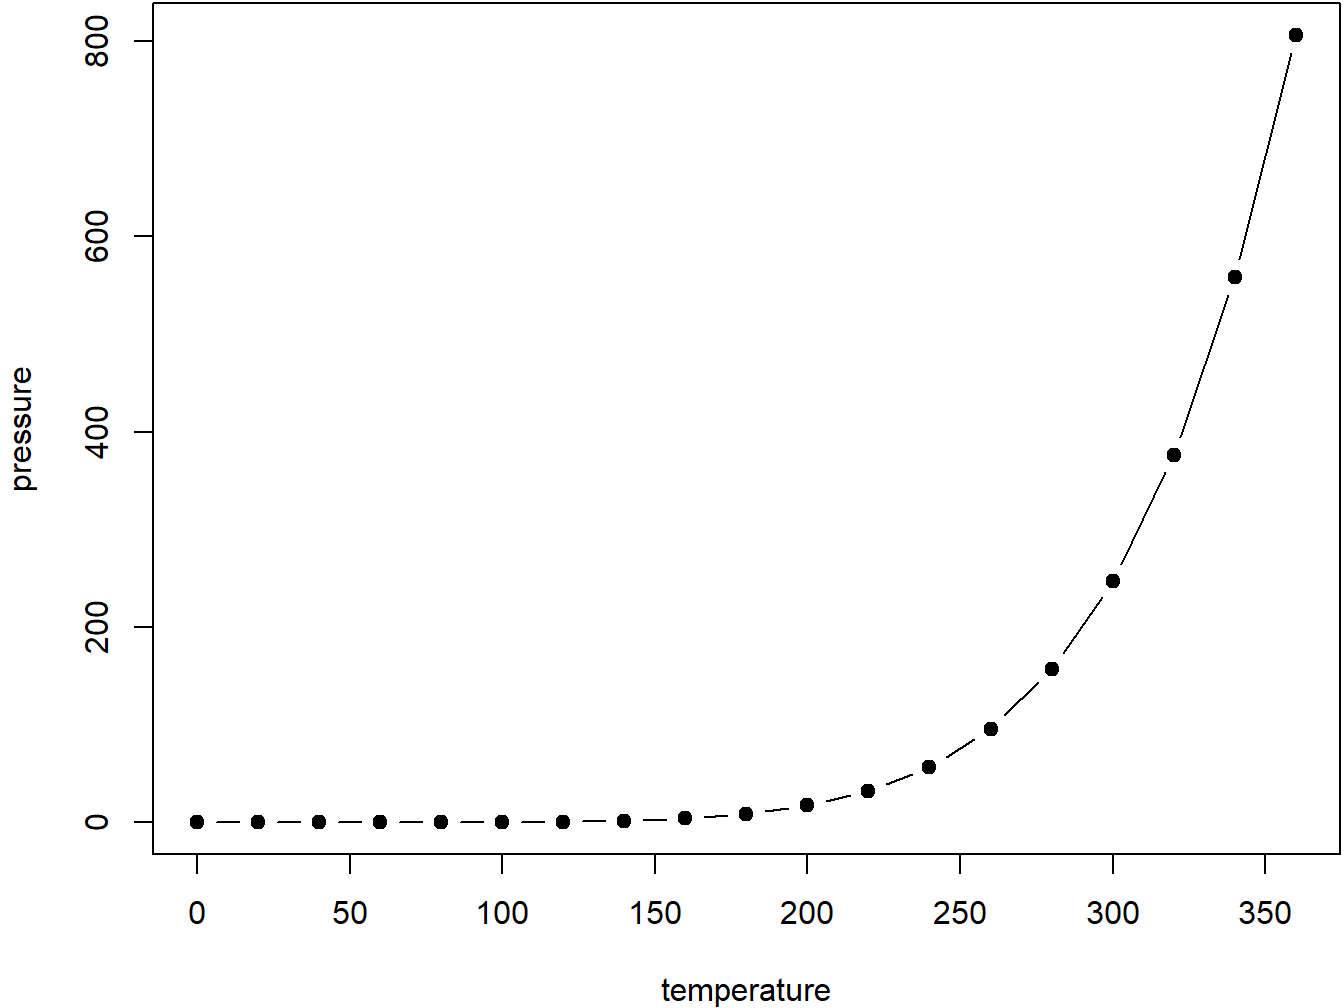
\includegraphics[width=0.8\linewidth]{qpad-book_files/figure-latex/nice-fig-1} 

}

\caption{Here is a nice figure!}\label{fig:nice-fig}
\end{figure}

Reference a figure by its code chunk label with the \texttt{fig:} prefix, e.g., see Figure \ref{fig:nice-fig}. Similarly, you can reference tables generated from \texttt{knitr::kable()}, e.g., see Table \ref{tab:nice-tab}.

\begin{Shaded}
\begin{Highlighting}[]
\NormalTok{knitr}\OperatorTok{::}\KeywordTok{kable}\NormalTok{(}
  \KeywordTok{head}\NormalTok{(iris, }\DecValTok{20}\NormalTok{), }\DataTypeTok{caption =} \StringTok{'Here is a nice table!'}\NormalTok{,}
  \DataTypeTok{booktabs =} \OtherTok{TRUE}
\NormalTok{)}
\end{Highlighting}
\end{Shaded}

\begin{table}[t]

\caption{\label{tab:nice-tab}Here is a nice table!}
\centering
\begin{tabular}{rrrrl}
\toprule
Sepal.Length & Sepal.Width & Petal.Length & Petal.Width & Species\\
\midrule
5.1 & 3.5 & 1.4 & 0.2 & setosa\\
4.9 & 3.0 & 1.4 & 0.2 & setosa\\
4.7 & 3.2 & 1.3 & 0.2 & setosa\\
4.6 & 3.1 & 1.5 & 0.2 & setosa\\
5.0 & 3.6 & 1.4 & 0.2 & setosa\\
\addlinespace
5.4 & 3.9 & 1.7 & 0.4 & setosa\\
4.6 & 3.4 & 1.4 & 0.3 & setosa\\
5.0 & 3.4 & 1.5 & 0.2 & setosa\\
4.4 & 2.9 & 1.4 & 0.2 & setosa\\
4.9 & 3.1 & 1.5 & 0.1 & setosa\\
\addlinespace
5.4 & 3.7 & 1.5 & 0.2 & setosa\\
4.8 & 3.4 & 1.6 & 0.2 & setosa\\
4.8 & 3.0 & 1.4 & 0.1 & setosa\\
4.3 & 3.0 & 1.1 & 0.1 & setosa\\
5.8 & 4.0 & 1.2 & 0.2 & setosa\\
\addlinespace
5.7 & 4.4 & 1.5 & 0.4 & setosa\\
5.4 & 3.9 & 1.3 & 0.4 & setosa\\
5.1 & 3.5 & 1.4 & 0.3 & setosa\\
5.7 & 3.8 & 1.7 & 0.3 & setosa\\
5.1 & 3.8 & 1.5 & 0.3 & setosa\\
\bottomrule
\end{tabular}
\end{table}

\hypertarget{binomial-model-and-censoring}{%
\section{Binomial model and censoring}\label{binomial-model-and-censoring}}

Try cloglog with a rare species, like BOCH

\begin{Shaded}
\begin{Highlighting}[]
\CommentTok{#spp <- "OVEN" # which species}
\NormalTok{spp <-}\StringTok{ "BOCH"} \CommentTok{# which species}
\CommentTok{#spp <- "CAWA" # which species}

\NormalTok{x <-}\StringTok{ }\KeywordTok{data.frame}\NormalTok{(}
\NormalTok{  josm}\OperatorTok{$}\NormalTok{surveys, }
  \DataTypeTok{y=}\KeywordTok{as.numeric}\NormalTok{(ytot[}\KeywordTok{rownames}\NormalTok{(x), spp]))}
\NormalTok{x}\OperatorTok{$}\NormalTok{y01 <-}\StringTok{ }\KeywordTok{ifelse}\NormalTok{(x}\OperatorTok{$}\NormalTok{y }\OperatorTok{>}\StringTok{ }\DecValTok{0}\NormalTok{, }\DecValTok{1}\NormalTok{, }\DecValTok{0}\NormalTok{)}

\KeywordTok{table}\NormalTok{(x}\OperatorTok{$}\NormalTok{y)}


\NormalTok{mP <-}\StringTok{ }\KeywordTok{glm}\NormalTok{(y }\OperatorTok{~}\StringTok{ }\NormalTok{Decid }\OperatorTok{*}\StringTok{ }\NormalTok{ConifWet, x, }\DataTypeTok{family=}\NormalTok{poisson)}
\NormalTok{mBc <-}\StringTok{ }\KeywordTok{glm}\NormalTok{(y01 }\OperatorTok{~}\StringTok{ }\NormalTok{Decid }\OperatorTok{*}\StringTok{ }\NormalTok{ConifWet, x, }\DataTypeTok{family=}\KeywordTok{binomial}\NormalTok{(}\StringTok{"cloglog"}\NormalTok{))}
\NormalTok{mBl <-}\StringTok{ }\KeywordTok{glm}\NormalTok{(y01 }\OperatorTok{~}\StringTok{ }\NormalTok{Decid }\OperatorTok{*}\StringTok{ }\NormalTok{ConifWet, x, }\DataTypeTok{family=}\KeywordTok{binomial}\NormalTok{(}\StringTok{"logit"}\NormalTok{))}

\KeywordTok{coef}\NormalTok{(mP)}
\KeywordTok{coef}\NormalTok{(mBc)}
\KeywordTok{coef}\NormalTok{(mBl)}

\KeywordTok{plot}\NormalTok{(}\KeywordTok{fitted}\NormalTok{(mBc) }\OperatorTok{~}\StringTok{ }\KeywordTok{fitted}\NormalTok{(mP), }\DataTypeTok{col=}\DecValTok{4}\NormalTok{, }
  \DataTypeTok{ylim=}\KeywordTok{c}\NormalTok{(}\DecValTok{0}\NormalTok{, }\KeywordTok{max}\NormalTok{(}\KeywordTok{fitted}\NormalTok{(mP))), }\DataTypeTok{xlim=}\KeywordTok{c}\NormalTok{(}\DecValTok{0}\NormalTok{, }\KeywordTok{max}\NormalTok{(}\KeywordTok{fitted}\NormalTok{(mP))))}
\KeywordTok{points}\NormalTok{(}\KeywordTok{exp}\NormalTok{(}\KeywordTok{model.matrix}\NormalTok{(mBc) }\OperatorTok\StringTok{ }\KeywordTok{coef}\NormalTok{(mBc)) }\OperatorTok{~}\StringTok{ }\KeywordTok{fitted}\NormalTok{(mP), }\DataTypeTok{col=}\DecValTok{2}\NormalTok{)}
\KeywordTok{abline}\NormalTok{(}\DecValTok{0}\NormalTok{,}\DecValTok{1}\NormalTok{)}
\end{Highlighting}
\end{Shaded}

\hypertarget{optimal-partitioning}{%
\section{Optimal partitioning}\label{optimal-partitioning}}

\begin{Shaded}
\begin{Highlighting}[]
\NormalTok{oc <-}\StringTok{ }\KeywordTok{opticut}\NormalTok{(}\KeywordTok{as.matrix}\NormalTok{(ytot) }\OperatorTok{~}\StringTok{ }\DecValTok{1}\NormalTok{, }\DataTypeTok{strata =}\NormalTok{ x}\OperatorTok{$}\NormalTok{HAB, }\DataTypeTok{dist=}\StringTok{"poisson"}\NormalTok{)}
\KeywordTok{plot}\NormalTok{(oc)}
\end{Highlighting}
\end{Shaded}

\hypertarget{optilevels}{%
\section{Optilevels}\label{optilevels}}

When we have categorical or compositional (when e.g.~proportions add up to 1, also called
the unit sum constraint) data,
we often want to simplify and merge classes or add up columns.
We can do this based on the structural understanding of these land cover classes
(call all treed classes Forest, like what we did for \texttt{FOR}, \texttt{WET} and \texttt{AHF}).

Alternatively, we can let the data (the birds) tell us how to merge the classes.
The algorithm does the following:

\begin{enumerate}
\def\labelenumi{\arabic{enumi}.}
\tightlist
\item
  fit model with all classes,
\item
  order estimates for each class from smallest to largest,
\item
  merge classes that are near each others, 2 at a time, moving from smallest to largest,
\item
  compare \(\Delta\)AIC or \(\Delta\)BIC values for the merged models and pick the smallest,
\item
  treat this best merged model as an input in step 1 and star over until \(\Delta\) is negative (no improvement).
\end{enumerate}

Here is the code for simplifying categories using the \texttt{opticut::optilevels} function:

\begin{Shaded}
\begin{Highlighting}[]
\NormalTok{M <-}\StringTok{ }\KeywordTok{model.matrix}\NormalTok{(}\OperatorTok{~}\NormalTok{HAB}\DecValTok{-1}\NormalTok{, x)}
\KeywordTok{colnames}\NormalTok{(M) <-}\StringTok{ }\KeywordTok{levels}\NormalTok{(x}\OperatorTok{$}\NormalTok{HAB)}
\NormalTok{ol1 <-}\StringTok{ }\KeywordTok{optilevels}\NormalTok{(x}\OperatorTok{$}\NormalTok{y, M, }\DataTypeTok{dist=}\StringTok{"poisson"}\NormalTok{)}
\KeywordTok{sort}\NormalTok{(}\KeywordTok{exp}\NormalTok{(}\KeywordTok{coef}\NormalTok{(}\KeywordTok{bestmodel}\NormalTok{(ol1))))}
\CommentTok{## estimates}
\KeywordTok{exp}\NormalTok{(ol1}\OperatorTok{$}\NormalTok{coef)}
\CommentTok{## optimal classification}
\NormalTok{ol1}\OperatorTok{$}\NormalTok{rank}
\KeywordTok{data.frame}\NormalTok{(}\DataTypeTok{combined_levels=}\NormalTok{ol1}\OperatorTok{$}\NormalTok{levels[[}\KeywordTok{length}\NormalTok{(ol1}\OperatorTok{$}\NormalTok{levels)]])}
\end{Highlighting}
\end{Shaded}

Here is the code for simplifying compositional data:

\begin{Shaded}
\begin{Highlighting}[]
\NormalTok{ol2 <-}\StringTok{ }\KeywordTok{optilevels}\NormalTok{(x}\OperatorTok{$}\NormalTok{y, x[,cn], }\DataTypeTok{dist=}\StringTok{"poisson"}\NormalTok{)}
\KeywordTok{sort}\NormalTok{(}\KeywordTok{exp}\NormalTok{(}\KeywordTok{coef}\NormalTok{(}\KeywordTok{bestmodel}\NormalTok{(ol2))))}
\CommentTok{## estimates}
\KeywordTok{exp}\NormalTok{(ol2}\OperatorTok{$}\NormalTok{coef)}
\CommentTok{## optimal classification}
\NormalTok{ol2}\OperatorTok{$}\NormalTok{rank}
\KeywordTok{head}\NormalTok{(}\KeywordTok{groupSums}\NormalTok{(}\KeywordTok{as.matrix}\NormalTok{(x[,cn]), }\DecValTok{2}\NormalTok{, ol2}\OperatorTok{$}\NormalTok{levels[[}\KeywordTok{length}\NormalTok{(ol2}\OperatorTok{$}\NormalTok{levels)]]))}
\end{Highlighting}
\end{Shaded}

\hypertarget{n-mixture-models}{%
\section{N-mixture models}\label{n-mixture-models}}

\hypertarget{estimating-abundance-1}{%
\section{Estimating abundance}\label{estimating-abundance-1}}

Exponential model, bSims data

\begin{Shaded}
\begin{Highlighting}[]
\KeywordTok{set.seed}\NormalTok{(}\DecValTok{1}\NormalTok{)}
\NormalTok{phi <-}\StringTok{ }\FloatTok{0.5}
\NormalTok{Den <-}\StringTok{ }\DecValTok{1}
\NormalTok{l <-}\StringTok{ }\KeywordTok{bsims_init}\NormalTok{()}
\NormalTok{a <-}\StringTok{ }\KeywordTok{bsims_populate}\NormalTok{(l, }\DataTypeTok{density=}\NormalTok{Den)}
\NormalTok{b <-}\StringTok{ }\KeywordTok{bsims_animate}\NormalTok{(a, }\DataTypeTok{vocal_rate=}\NormalTok{phi, }\DataTypeTok{move_rate=}\DecValTok{0}\NormalTok{)}

\NormalTok{tint <-}\StringTok{ }\DecValTok{1}\OperatorTok{:}\DecValTok{5}
\NormalTok{(tr <-}\StringTok{ }\KeywordTok{bsims_transcribe}\NormalTok{(b, }\DataTypeTok{tint=}\NormalTok{tint))}
\end{Highlighting}
\end{Shaded}

\begin{verbatim}
## bSims transcript
##   1 km x 1 km
##   stratification: H
##   total abundance: 104
##   total duration: 10
##   detected: 104 heard
##   1st inds. [0-1, 1-2, 2-3, 3-4, 4-5 min] [0+ m]
\end{verbatim}

Multiple-visit stuff for bSims: the counting of new individuals
resets for each interval (also: needs equal intervals)

\begin{Shaded}
\begin{Highlighting}[]
\NormalTok{tr}\OperatorTok{$}\NormalTok{visits}
\end{Highlighting}
\end{Shaded}

\begin{verbatim}
##     0-1min 1-2min 2-3min 3-4min 4-5min
## 0+m     35     48     44     43     45
\end{verbatim}

\begin{Shaded}
\begin{Highlighting}[]
\NormalTok{v <-}\StringTok{ }\KeywordTok{get_events}\NormalTok{(b, }\DataTypeTok{vocal_only=}\OtherTok{TRUE}\NormalTok{)}
\NormalTok{v <-}\StringTok{ }\NormalTok{v[v}\OperatorTok{$}\NormalTok{t }\OperatorTok{<=}\StringTok{ }\KeywordTok{max}\NormalTok{(tint),]}
\NormalTok{v1 <-}\StringTok{ }\NormalTok{v[}\OperatorTok{!}\KeywordTok{duplicated}\NormalTok{(v}\OperatorTok{$}\NormalTok{i),]}

\NormalTok{tmp <-}\StringTok{ }\NormalTok{v1}
\NormalTok{tmp}\OperatorTok{$}\NormalTok{o <-}\StringTok{ }\KeywordTok{seq_len}\NormalTok{(}\KeywordTok{nrow}\NormalTok{(v1))}
\KeywordTok{plot}\NormalTok{(o }\OperatorTok{~}\StringTok{ }\NormalTok{t, tmp, }\DataTypeTok{type=}\StringTok{"n"}\NormalTok{, }\DataTypeTok{ylab=}\StringTok{"Individuals"}\NormalTok{,}
  \DataTypeTok{main=}\StringTok{"Vocalization events"}\NormalTok{, }
  \DataTypeTok{ylim=}\KeywordTok{c}\NormalTok{(}\DecValTok{1}\NormalTok{, }\KeywordTok{nrow}\NormalTok{(b}\OperatorTok{$}\NormalTok{nests)), }\DataTypeTok{xlim=}\KeywordTok{c}\NormalTok{(}\DecValTok{0}\NormalTok{,}\KeywordTok{max}\NormalTok{(tint)))}
\ControlFlowTok{for}\NormalTok{ (i }\ControlFlowTok{in}\NormalTok{ tmp}\OperatorTok{$}\NormalTok{o) \{}
\NormalTok{  tmp2 <-}\StringTok{ }\NormalTok{v[v}\OperatorTok{$}\NormalTok{i }\OperatorTok{==}\StringTok{ }\NormalTok{v1}\OperatorTok{$}\NormalTok{i[i],]}
  \KeywordTok{lines}\NormalTok{(}\KeywordTok{c}\NormalTok{(tmp2}\OperatorTok{$}\NormalTok{t[}\DecValTok{1}\NormalTok{], }\KeywordTok{max}\NormalTok{(tint)), }\KeywordTok{c}\NormalTok{(i,i), }\DataTypeTok{col=}\StringTok{"grey"}\NormalTok{)}
  \KeywordTok{points}\NormalTok{(tmp2}\OperatorTok{$}\NormalTok{t, }\KeywordTok{rep}\NormalTok{(i, }\KeywordTok{nrow}\NormalTok{(tmp2)), }\DataTypeTok{cex=}\FloatTok{0.5}\NormalTok{)}
  \KeywordTok{points}\NormalTok{(tmp2}\OperatorTok{$}\NormalTok{t[}\DecValTok{1}\NormalTok{], i, }\DataTypeTok{pch=}\DecValTok{19}\NormalTok{, }\DataTypeTok{cex=}\FloatTok{0.5}\NormalTok{)}
\NormalTok{\}}
\end{Highlighting}
\end{Shaded}

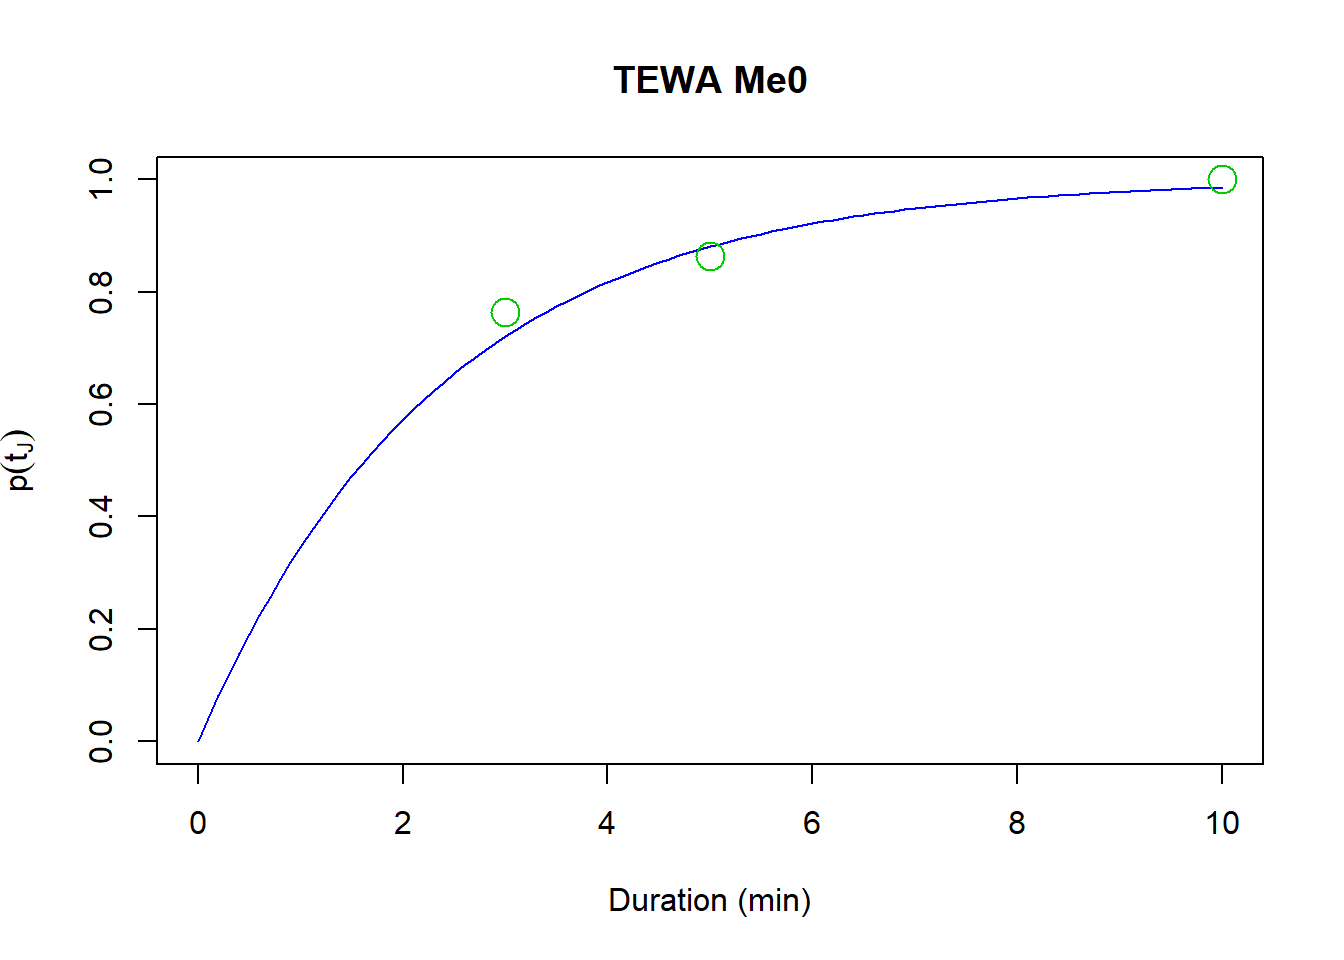
\includegraphics{qpad-book_files/figure-latex/unnamed-chunk-79-1.pdf}

\begin{Shaded}
\begin{Highlighting}[]
\KeywordTok{plot}\NormalTok{(o }\OperatorTok{~}\StringTok{ }\NormalTok{t, tmp, }\DataTypeTok{type=}\StringTok{"n"}\NormalTok{, }\DataTypeTok{ylab=}\StringTok{"Individuals"}\NormalTok{,}
  \DataTypeTok{main=}\StringTok{"Vocalization events"}\NormalTok{, }
  \DataTypeTok{ylim=}\KeywordTok{c}\NormalTok{(}\DecValTok{1}\NormalTok{, }\KeywordTok{nrow}\NormalTok{(b}\OperatorTok{$}\NormalTok{nests)), }\DataTypeTok{xlim=}\KeywordTok{c}\NormalTok{(}\DecValTok{0}\NormalTok{,}\KeywordTok{max}\NormalTok{(tint)))}
\ControlFlowTok{for}\NormalTok{ (j }\ControlFlowTok{in} \KeywordTok{seq_along}\NormalTok{(tint)) \{}
\NormalTok{  ii <-}\StringTok{ }\ControlFlowTok{if}\NormalTok{ (j }\OperatorTok{==}\StringTok{ }\DecValTok{1}\NormalTok{)}
    \KeywordTok{c}\NormalTok{(}\DecValTok{0}\NormalTok{, tint[j]) }\ControlFlowTok{else} \KeywordTok{c}\NormalTok{(tint[j}\DecValTok{-1}\NormalTok{], tint[j])}
\NormalTok{  vv <-}\StringTok{ }\NormalTok{v[v}\OperatorTok{$}\NormalTok{t }\OperatorTok{>}\StringTok{ }\NormalTok{ii[}\DecValTok{1}\NormalTok{] }\OperatorTok{&}\StringTok{ }\NormalTok{v}\OperatorTok{$}\NormalTok{t }\OperatorTok{<=}\StringTok{ }\NormalTok{ii[}\DecValTok{2}\NormalTok{],]}
\NormalTok{  tmp <-}\StringTok{ }\NormalTok{vv[}\OperatorTok{!}\KeywordTok{duplicated}\NormalTok{(vv}\OperatorTok{$}\NormalTok{i),]}
\NormalTok{  tmp}\OperatorTok{$}\NormalTok{o <-}\StringTok{ }\KeywordTok{seq_len}\NormalTok{(}\KeywordTok{nrow}\NormalTok{(tmp))}
  \ControlFlowTok{if}\NormalTok{ (}\KeywordTok{nrow}\NormalTok{(tmp)) \{}
    \ControlFlowTok{for}\NormalTok{ (i }\ControlFlowTok{in}\NormalTok{ tmp}\OperatorTok{$}\NormalTok{o) \{}
\NormalTok{      tmp2 <-}\StringTok{ }\NormalTok{vv[vv}\OperatorTok{$}\NormalTok{i }\OperatorTok{==}\StringTok{ }\NormalTok{tmp}\OperatorTok{$}\NormalTok{i[i],]}
      \KeywordTok{lines}\NormalTok{(}\KeywordTok{c}\NormalTok{(tmp2}\OperatorTok{$}\NormalTok{t[}\DecValTok{1}\NormalTok{], ii[}\DecValTok{2}\NormalTok{]), }\KeywordTok{c}\NormalTok{(i,i), }\DataTypeTok{col=}\StringTok{"grey"}\NormalTok{)}
      \KeywordTok{points}\NormalTok{(tmp2}\OperatorTok{$}\NormalTok{t, }\KeywordTok{rep}\NormalTok{(i, }\KeywordTok{nrow}\NormalTok{(tmp2)), }\DataTypeTok{cex=}\FloatTok{0.5}\NormalTok{)}
      \KeywordTok{points}\NormalTok{(tmp2}\OperatorTok{$}\NormalTok{t[}\DecValTok{1}\NormalTok{], i, }\DataTypeTok{pch=}\DecValTok{19}\NormalTok{, }\DataTypeTok{cex=}\FloatTok{0.5}\NormalTok{)}
\NormalTok{    \}}
\NormalTok{  \}}
\NormalTok{\}}
\end{Highlighting}
\end{Shaded}

\includegraphics{qpad-book_files/figure-latex/unnamed-chunk-79-2.pdf}

\begin{Shaded}
\begin{Highlighting}[]
\KeywordTok{library}\NormalTok{(unmarked)}

\NormalTok{f <-}\StringTok{ }\ControlFlowTok{function}\NormalTok{() \{}
\NormalTok{  a <-}\StringTok{ }\KeywordTok{bsims_populate}\NormalTok{(l, }\DataTypeTok{density=}\NormalTok{Den)}
\NormalTok{  b <-}\StringTok{ }\KeywordTok{bsims_animate}\NormalTok{(a, }\DataTypeTok{vocal_rate=}\NormalTok{phi, }\DataTypeTok{move_rate=}\DecValTok{0}\NormalTok{)}
\NormalTok{  tr <-}\StringTok{ }\KeywordTok{bsims_transcribe}\NormalTok{(b, }\DataTypeTok{tint=}\NormalTok{tint)}
  \KeywordTok{drop}\NormalTok{(tr}\OperatorTok{$}\NormalTok{visits)}
\NormalTok{\}}

\NormalTok{Den <-}\StringTok{ }\FloatTok{0.01}

\CommentTok{#ymx <- tr$visits}
\NormalTok{(ymx <-}\StringTok{ }\KeywordTok{t}\NormalTok{(}\KeywordTok{replicate}\NormalTok{(}\DecValTok{10}\NormalTok{, }\KeywordTok{f}\NormalTok{())))}
\end{Highlighting}
\end{Shaded}

\begin{verbatim}
##       0-1min 1-2min 2-3min 3-4min 4-5min
##  [1,]      0      0      0      0      0
##  [2,]      0      1      0      0      1
##  [3,]      0      2      2      1      0
##  [4,]      1      1      0      1      0
##  [5,]      0      0      0      0      0
##  [6,]      0      0      0      0      0
##  [7,]      2      2      0      1      0
##  [8,]      1      1      0      0      0
##  [9,]      0      0      0      0      0
## [10,]      0      1      0      1      0
\end{verbatim}

\begin{Shaded}
\begin{Highlighting}[]
\CommentTok{## highly dependent on K when Den is higher}
\NormalTok{nmix <-}\StringTok{ }\KeywordTok{pcount}\NormalTok{(}\OperatorTok{~}\DecValTok{1} \OperatorTok{~}\DecValTok{1}\NormalTok{, }\KeywordTok{unmarkedFramePCount}\NormalTok{(}\DataTypeTok{y=}\NormalTok{ymx), }\DataTypeTok{K=}\DecValTok{1000}\NormalTok{)}
\KeywordTok{coef}\NormalTok{(nmix)}
\end{Highlighting}
\end{Shaded}

\begin{verbatim}
## lam(Int)   p(Int) 
## -0.02602 -0.44730
\end{verbatim}

\begin{Shaded}
\begin{Highlighting}[]
\KeywordTok{plogis}\NormalTok{(}\KeywordTok{coef}\NormalTok{(nmix)[}\DecValTok{2}\NormalTok{])}
\end{Highlighting}
\end{Shaded}

\begin{verbatim}
## p(Int) 
##   0.39
\end{verbatim}

\begin{Shaded}
\begin{Highlighting}[]
\KeywordTok{exp}\NormalTok{(}\KeywordTok{coef}\NormalTok{(nmix)[}\DecValTok{1}\NormalTok{])}
\end{Highlighting}
\end{Shaded}

\begin{verbatim}
## lam(Int) 
##   0.9743
\end{verbatim}

\begin{Shaded}
\begin{Highlighting}[]
\NormalTok{Den }\OperatorTok{*}\StringTok{ }\DecValTok{100}
\end{Highlighting}
\end{Shaded}

\begin{verbatim}
## [1] 1
\end{verbatim}

\bibliography{book.bib,packages.bib,publications.bib}


\end{document}
